\documentclass[12pt]{book}

\usepackage[utf8]{inputenc}
\usepackage[T1]{fontenc}
\usepackage[brazil]{babel}
\usepackage{anyfontsize}
\usepackage{mathptmx}
\usepackage{gensymb}
\usepackage{indentfirst}
\usepackage{mdframed}
\usepackage{hhline}
\usepackage{graphicx}
\usepackage{chngcntr}
\usepackage{enumitem}
\usepackage{amsmath}
\usepackage{amsthm,amssymb}
\usepackage{xparse}
\usepackage{xcolor}
\usepackage{color, soul}
\usepackage{amsthm}
\usepackage{tabto}
\usepackage{ragged2e}
\usepackage{float}
\usepackage{changepage}
\usepackage{multicol}
\usepackage{tikz}
\usepackage[left=3cm,right=2cm,top=3cm,bottom=2cm]{geometry}
\usepackage{varioref}
\usepackage[colorlinks=true]{hyperref}
\usepackage[nameinlink]{cleveref}

%%capa%%
\title{
\includegraphics[scale=1]{recursos/logo_uffs.pdf}\\ Livro Matemática C}
\author{Pedro Borges}
\date{MARÇO/2015}
%%capa%%

%%definições
\theoremstyle{definition}

\newlength\widest
\counterwithin{figure}{section}

\renewcommand{\qedsymbol}{\rule{0.7em}{0.7em}}
\renewcommand{\contentsname}{Sumário}
\renewcommand{\figurename}{Figura}
\newcommand\myrule[1]{\multicolumn{1}{| l}{#1}}

\setlength\parindent{1em}
\setlength\parskip{0.5em}
%%definições

%%hyperlinks%%
\newcommand{\exitem}[1]{
    \refstepcounter{enumi}
    \item[{\hyperref[ans:\theenumi]{\theenumi}}]#1 \label{ex:\theenumi}
}
\newcommand{\ansitem}[1]{
    \refstepcounter{enumi}
    \item[{\hyperref[ex:\theenumi]{\theenumi}}]#1 \label{ans:\theenumi}
}
%\usepackage{showlabels}
%%hyperlinks%%

%%envs%%
\newtheorem{texemplo}{Exemplo}[section]
\newtheorem{tdefinicao}{Definição}[section]

\newcounter{eqcnt}[chapter]
\newcommand{\equacao}[1]{
    \stepcounter{eqcnt}
    \begin{multicols}{2}
    #1
    
    (\thechapter.\theeqcnt) \label{eqc:\thechapter.\theeqcnt}
    \end{multicols}
}

\mdfdefinestyle{MyFrame}{%
    linecolor=black,
    outerlinewidth=2pt,
    %roundcorner=20pt,
    innertopmargin=4pt,
    innerbottommargin=4pt,
    innerrightmargin=4pt,
    innerleftmargin=4pt,
        leftmargin = 4pt,
        rightmargin = 4pt
    %backgroundcolor=gray!50!white}
}

\newenvironment{exercicios}
{
    \noindent\textbf{EXERCÍCIOS \thesection}
    \begin{enumerate}[label=\thesection.\arabic*]
}
{
    \end{enumerate}
}

\newenvironment{respostas}[1]
{
    \noindent\textbf{RESPOSTAS \thechapter.#1}
    \begin{enumerate}[label=\thechapter.#1.\arabic*]
}
{
    \end{enumerate}
}

\newenvironment{caixa}
{
    \begin{mdframed}[style=MyFrame,nobreak=true]
    \begin{center}
}
{
    \end{center}
    \end{mdframed}
}
%%envs%%

\begin{document}

\maketitle

\tableofcontents
\clearpage

\chapter{Conjuntos Numéricos}
\section{Introdução}

A criação dos números, como conhecemos hoje, é produto da evolução de ideias sobre como representar determinadas grandezas, resolver problemas geométricos, problemas aplicados às ciências e resolução de equações. 

A noção de número inteiro foi criada pela necessidade de contar objetos, animais e pessoas. Nossos antepassados contavam somente até dois, a partir disto, o conjunto de coisas era dado como "muitos" (BOYER, p.2). Alguns índios, até hoje, têm dificuldades em contar até três (KARLSON, p.5). Inicialmente o homem contava com os dedos, com grãos, com pequenas pedras ou fazendo marcas em bastões, relacionando a eles os objetos de seu interesse: uma pedra, um búfalo; uma família, os dedos de uma mão. É a contagem por correspondência um a um.

Cada cultura desenvolveu uma representação simbólica. Os egípcios, antes de 5.000 a.C. usavam um sistema de numeração com barras e figuras para resolver problemas bem mais complexos do que a simples contagem. Os romanos criaram um sistema de representação com letras, mas com limitações para efetuar operações. Os hindus, por volta de 595 d.C. usavam nove símbolos, e dois séculos depois, incluíram o zero, completando um sistema de numeração posicional, com algoritmos eficientes para operações, que os árabes divu/lgaram pela Europa, mais tarde. 

Problemas de comércio e contabilidade motivaram o uso de sinais em números para representar ganhos e perdas. Diofanto já operava com negativos, no século III. 

Os povos antigos (egípcios, mesopotâmios, hindus e chineses) enunciaram e resolveram problemas algébricos e geométricos, cujas soluções era não inteira, evidenciando o conhecimento e uso de números fracionários. Os pitagóricos (século V a.C.) não conseguiram explicar a natureza do número que representa a medida da diagonal de um quadrado e com isso geraram a necessidade de criar números não racionais. 

Durante o século XIX e século XX o movimento de axiomatização da matemática levou à construção dos conjuntos numéricos, com base na teoria dos conjuntos. Tal construção foi desenvolvida por Giuseppe Peano. 

O conhecimento sobre a natureza dos números é importante para as ciências puras e aplicadas, apesar do senso comum reduzir as aplicações a números inteiros ou fracionários (no sentido de não inteiro). O número de funcionários de uma empresa, de carros, de pizzas, de sapatos, de vacas, ..., são quantidades inteiras. Não se pode considerar meio funcionário, meio carro ou meia vaca. O tempo, os valores monetários, o número de toneladas (massa) de arroz, soja, feijão, ..., são variáveis fracionárias. Trabalhamos com meia hora, com meio dólar, etc. Porém, o comprimento da hipotenusa de uma tesoura triangular de telhado pode ser aproximado por um número fracionário finito, mas é um número irracional, para a grande maioria dos casos. Da mesma forma, grandezas da eletricidade requerem a definição de números não reais, chamados de complexos. Assim, para entendermos as expressões matemáticas das variáveis, com clareza e precisão, precisamos conhecer os tipos de números, suas propriedades e operações.

\section{Conjunto dos Números Naturais ($\mathbb{N}$)}

A contagem de quantidades inteiras de animais, pessoas ou coisas, foi provavelmente, o que motivou a criação dos números naturais.

$$ \mathbb{N} = \{ 0,1,2,3,4,... \}$$

O conjunto dos números naturais é infinito e pode ser representado em uma reta numerada com pontos cheios:

\begin{figure}[H]
	\begin{Center}
		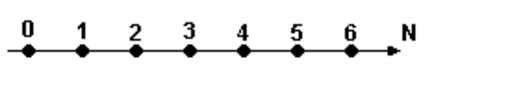
\includegraphics[width=3.44in,height=0.58in]{capitulos/conjuntos_numericos/media/image2.pdf}
	\end{Center}
\end{figure}

~~

Os intervalos no conjunto dos números naturais são escritos usando os símbolos 

> maior 

< menor 

$\geq$ maior ou igual e

$\leq$ menor ou igual.

Vejamos os exemplos:

\begin{texemplo}
	
	Escreva os elementos do conjunto  A=$ \{ x \in \mathbb{N}  / x > 2 \} $  (Lê-se: x pertence aos Naturais, tal que x é maior do que 2) e represente-os em uma reta.

\textbf{Solução}: Escrevendo os elementos de A, temos: A= $ \{ 3,4,5,6,7,... \}$.

Mostrando esse conjunto na reta dos números naturais, colocamos pontos cheios pretos para os elementos do conjunto \textbf{A e vazios para os elementos que não pertencem ao conjunto A.}

\begin{figure}[H]
	\begin{Center}
		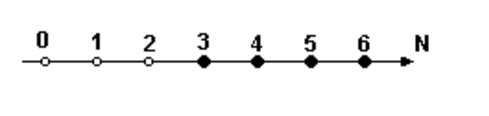
\includegraphics[width=3.26in,height=0.77in]{capitulos/conjuntos_numericos/media/image3.pdf}
	\end{Center}
\end{figure}

~~
\end{texemplo}

\begin{texemplo} 
	Escreva os elementos do conjunto~ B=$ \{ x \in \mathbb{N}  / 1< x <5 \} $  ( Lê-se: x pertence aos Naturais, tal que x é maior do que 1 e menor do que 5. (ou, x pertence aos Naturais , tal que 1 é menor do que x e x é menor do que 5) e represente-os em uma reta.

\textbf{Solução:} Usando a mesma representação do Exemplo 2.1, temos: B=$ \{ 2,3,4 \} $. Mostrando esse conjunto na reta dos números naturais, temos:

\begin{figure}[H]
	\begin{Center}
		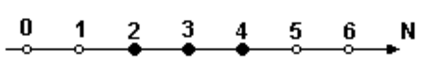
\includegraphics[width=2.93in,height=0.45in]{capitulos/conjuntos_numericos/media/image4.pdf}
	\end{Center}
\end{figure}
\end{texemplo}

\begin{texemplo}
Escreva os elementos do conjunto C, representado na reta numerada:

\begin{figure}[H]
	\begin{Center}
		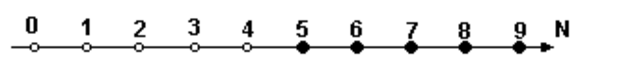
\includegraphics[width=4.17in,height=0.51in]{capitulos/conjuntos_numericos/media/image5.pdf}
	\end{Center}
\end{figure}

\textbf{Solução:}\quad Podemos escrever os elementos desse conjunto de duas maneiras: por extensão (descrevendo um a um) 

$$ C=\{5,6,7,8,9,10,\dots\}$$

\quad ou usando os símbolos de desigualdade  

\quad $C= \{ x \in \mathbb{N} / x  5 \}$ ou ainda $C= \{ x \in \mathbb{N} / x > 4 \}$ \qedsymbol{}
\end{texemplo}

\begin{exercicios}
    \exitem{} Escreva por extensão os elementos dos conjuntos:
    \begin{multicols}{2}
        a) A=$ \{x \in \mathbb{N} / x > 5 \}$ 

        b) B=$ \{ x \in \mathbb{N} / 1 < x < 10 \}$ 

        c) C=$ \{ x \in \mathbb{N} / x \leq 6 \} $
        
        d) D=$ \{ x \in \mathbb{N} / 2 \leq x < 8 \} $
        
        e) E=$ \{x \in \mathbb{N} / 2 < x \leq 5 \}$
        
        f) F=$ \{x \in \mathbb{N} / 2 > x \textrm{ ou } x > 5 \}$
    \end{multicols}
	\exitem{} Represente os conjuntos do Ex.1 graficamente.

	\exitem{} Verifique se as quantidades das grandezas abaixo podem ser expressas com números naturais:

        a) População de uma cidade.

        b) Número de porcos criados em uma granja por ano.

        c) A velocidade de uma pessoa em uma corrida de maratona.

        d) O número de escovas de dentes produzido mensalmente por uma indústria.

        e) A taxa de variação da cesta básica em um estado do Brasil em um determinado mês.

	\exitem{} As notas das provas escolares são expressas em números naturais?

	\exitem{} Existe um número \textbf{natural} X que somado com 5 dê 3? (ou seja: 5 + X = 3)

	\exitem{} Verifique se as operações abaixo geram números naturais:
    \begin{multicols}{2}
        a) 5 + 8 = 

        b) 3 – 5 =
        
        c) 5$\cdot$ 8
        
        d) 8 $\div$ 5 =
    \end{multicols}
\end{exercicios}

\section{Conjunto dos Números Inteiros Relativos ($\mathbb{Z}$)}

As letras (b) e (d) do Exercício 1.1.6 ilustram problemas de operações com números naturais cuja solução gera números não naturais. Portanto, é necessário admitir a existência de outros tipos de números.

Se as quantidades ou grandezas inteiras mudam seu significado de acordo com um referencial, pode-se representa-las usando um sinal e um número. Vejamos alguns exemplos:

\textbf{Saldo bancário:} se temos dinheiro depositado, dizemos que o saldo é positivo. Se gastamos mais dinheiro do que temos e o banco nos empresta, dizemos que o saldo é negativo. Assim, se o saldo é +3.500,00 reais, significa que temos esse montante na conta. A referência, é o saldo zero. Neste caso, não temos nada, mas também não devemos ao banco.

\textbf{Temperatura:} a temperatura é uma grandeza associada ao estado térmico de um corpo: Quanto mais calor o corpo possui, maior será a temperatura e quanto mais frio, menor. Pela escala Celsius, a referência é a temperatura da água congelada: 0 \textsuperscript{o}C. Assim, na madrugada de um dia de inverno podemos ter temperaturas negativas, como -5\textsuperscript{o}C e ao meio-dia, positivas, como + 15\textsuperscript{o}C.

\textbf{Taxas de variações:} as variações de cotação de moedas, como o dólar, por exemplo, são dadas usando a referência zero, ou seja quando não varia. Assim, +2  significa que o dólar 'caiu'. Essas taxas de variações são muito usadas na economia: na bolsa de valores para indicar a tendência das ações; nas análises de desempenho de empresas (crescimento/decrescimento). Na física, o sinal da velocidade de um corpo indica o sentido do deslocamento.

Os números inteiros relativos podem ser representados da seguinte forma: 

 $$(\mathbb{Z})  = \{\dots,-6,-5,-4-3,-2,-1,0,+1,+2,+3,+4,+5,+6,\dots\}$$

A representação gráfica do conjunto  \(\mathbb{Z}\)  é:

\begin{figure}[H]
	\begin{Center}
		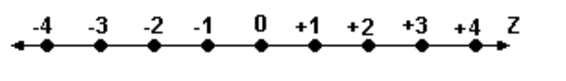
\includegraphics[width=3.77in,height=0.54in]{capitulos/conjuntos_numericos/media/image6.pdf}
	\end{Center}
\end{figure}

~~

Escrevendo o conjunto $\mathbb{Z}$  usando símbolos, temos: 

$\mathbb{Z} = \{x \in \mathbb{Z}/ -\infty < x < +\infty\}$.

\subsection{Operações em $\mathbb{Z}$}

\subsubsection{Adição e subtração de números inteiros}

Ao operar com números inteiros relativos, precisamos identificar inicialmente a operação solicitada e em seguida o sinal dos números.

\begin{figure}[H]
	\begin{Center}
		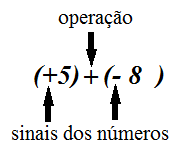
\includegraphics[width=1.88in,height=1.64in]{capitulos/conjuntos_numericos/media/image7.png}
	\end{Center}
\end{figure}

~~
\begin{center}
\textbf{Regra da adição de dois números inteiros}:
\end{center}

\begin{caixa}
    sinais iguais $\Rightarrow$ adiciona e usa o mesmo sinal no resultado

    sinais diferentes $\Rightarrow$ subtrai e usa o sinal do maior no resultado

\end{caixa}
\textbf{Exemplos:}
\begin{multicols}{2}
    1)$(+5) + (+3) = +5+3 = +8$ 

    2)$(+5) + (- 3) = +5 - 3 = +2$ 
    
    3)$(-5) + (+ 3) = -5 + 3 = -2$

    4)$(-5) + (- 3) = -5 - 3 = -8$
\end{multicols}
\subsubsection{Multiplicação e divisão de números inteiros}
 
\begin{center}
    \textbf{Regra da Subtração de dois números inteiros}
\end{center}
\begin{caixa}
Troca o sinal do segundo número e usa a regra da adição.
\end{caixa}
\textbf{Exemplos:}
\begin{multicols}{2}
1)$(+5) - (+ 3) = (+5) + (- 3) = +2$

2)$(+5) - (- 3) = (+5) + (+ 3) = +8$

3)$(-5) - (- 3) = (-5) + (+ 3) = - 2$

4)$(-5) - (+ 3) = (-5) + (- 3) = - 8$
\end{multicols}
\begin{center}
\textbf{Regra da Multiplicação e Divisão: }(para o sinal do resultado)
\end{center}
\begin{caixa}
sinais iguais $\Rightarrow$resultado positivo

sinais diferentes $\Rightarrow$resultado negativo
\end{caixa}

\textbf{Exemplos:}

\begin{multicols}{2}
	1)$(+5) \cdot (+4) = +20$

    2)$(+20) : (-4) = - 5$
    
    3)$ (+20) : (+4) = + 5$
    
    4)$(+5) \cdot (-4) = - 20$
\end{multicols}

\subsubsection{Potênciação de números inteiros}
 
\begin{caixa}
    \begin{tdefinicao}
    A potência~ \textit{b\textsuperscript{n}}~ , para  o expoente \textit{n $ \in $   \( \mathbb{N} \) } e a base \textit{b $ \in $   \( \mathbb{Z} \) ~ ,} é o produto de \textit{b}, \textit{n} vezes,  por ele mesmo:

    \begin{figure}[H]
	    \begin{Center}
		    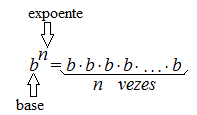
\includegraphics[width=2.05in,height=1.2in]{capitulos/conjuntos_numericos/media/image8.png}
	    \end{Center}
    \end{figure}
    \end{tdefinicao}
\end{caixa}

\textbf{Exemplos: }
Calcule (a) $2^4$, (b) $(-3)^3$, (c) $(-2)^4$ e (d) $-2^4$

\textbf{Solução}: 
\begin{enumerate}[label=\alph*]
    \item \textit{2\textsuperscript{4}}~=~2 $ \cdot $  2 $ \cdot $  2  $ \cdot $  2  = \textit{16}

    \item (-3)\textit{\textsuperscript{3}~ = (-3)} $ \cdot $  \textit{(-3)} $ \cdot $  \textit{(-3)} = \textit{-27}

    \item \textit{(-2)\textsuperscript{4} = (-2)} $ \cdot $  \textit{(-2)} $ \cdot $  \textit{(-2)} $ \cdot $  \textit{(-2)=~16  }

    \item -2\textit{\textsuperscript{4}~ = -2 }$ \cdot $  \textit{2} $ \cdot $  \textit{2} $ \cdot $ \textit{2 = -16}
\end{enumerate}

\textbf{Observemos que:}
\begin{caixa}
\begin{enumerate}
	\item Se a base é positiva (\textit{b > 0}) então \textit{b\textsuperscript{n}} > 0.

	\item Se a base é negativa (\textit{b < 0}) e :

    \quad Se \textit{n é par então b\textsuperscript{n} > 0}

    \quad Se \textit{n é ímpar então b\textsuperscript{n} < 0.}

	\item Se a base é 1 (\textit{b = 1}) então \textit{b\textsuperscript{n}} \textit{= 1}, para qualquer \textit{n $ \in $   \( \mathbb{N} \) .} 
\end{enumerate}
\end{caixa}

\subsubsection{Radiciação de números inteiros}
 
\begin{caixa}
    \begin{tdefinicao}
        A raiz \textit{n-ézima, }para\textit{ n }  \(\in \mathbb{\mathbb{N}} \)  , de um número \textit{b}   \(\in \mathbb{Z} \) é \textit{x}   \(\in \mathbb{Z} \)  se e somente se \textit{x\textsuperscript{n} = b}.
        \[ \sqrt[n]{b}=x \Longleftrightarrow   x^{n}=b. \]
    \end{tdefinicao}
\end{caixa}

\textbf{Exemplos}:

\begin{enumerate}
	\item  \( \sqrt[3]{8}=2~~ \Longleftrightarrow   2^{3}=8. \) 

	\item  \( \sqrt[3]{ \left( -8 \right) }=-2~~ \Longleftrightarrow    \left( -2 \right) ^{3}=-8. \) 

	\item  \( \sqrt[]{10}~~ \) não é um número inteiro, pois \textit{3\textsuperscript{2} < 10 < 4\textsuperscript{2}}.

	\item  \( \sqrt[]{4}=-2~~ \Longleftrightarrow    \left( -2 \right) ^{2}=4 \) ,~mas também   \( \sqrt[]{4}=2~~ \Longleftrightarrow    \left( 2 \right) ^{2}=4 \) . 
\end{enumerate}

Então~  \( \sqrt[]{4}= \pm ~2   \) \qedsymbol{}

\begin{exercicios}

	\exitem{} Resolva as expressões numéricas:
    \begin{multicols}{2}
        a)$(+15)+(-12) =$
        
        b)$(-15)+(-10) =$

        c)$(+8)+(-12)-(+5) =$
        
        d)$(-7)-(-9)-(+3) =$

        e)$(+6) : (-3) =$
        
        f)$(-7) \cdot (-5) =$

        g)$1- (-3)+(-4)=$
        
        h)$-4-[3+5(5 - 2)]=$

        i)$3\cdot(5 - 8)-(8 - 3)+6 =$
        
        j)$-[-4 -3\cdot(7-4)-(2-5)]=$
    \end{multicols}
	\exitem{} O saldo bancário de um correntista no dia 1\textsuperscript{o }do mês era de R$\$$  3.500,00 e no dia 3, entrou um cheque para ser descontado de R$\$$  4.350,00. Qual é o saldo no dia 3 ?

	\exitem{} Expresse e resolva as seguintes situações, usando números relativos:

    \quad a) Uma pessoa tem $50$ reais e \textbf{perde} $30$ reais.

    \quad b) Uma pessoa tem $100$ reais e \textbf{paga} uma dívida $40$.

    \quad c) Uma pessoa tem uma \textbf{dívida} de $100$ reais e \textbf{ganha} $50$ reais.

    \quad d) Uma pessoa tem uma \textbf{dívida} de $200$ reais e \textbf{perde} $70$ reais.

	\exitem{} Em um dia de inverno a temperatura máxima foi de \textit{18\textsuperscript{o}C} e a mínima de \textit{-3\textsuperscript{o}C}. Qual foi a variação de temperatura?

	\exitem{} Uma peça de metal estava a 80\textsuperscript{o}C e foi resfriada variando sua temperatura em 90\textsuperscript{o}C. Qual é a temperatura final da peça?

	\exitem{} Considere o nível do mar como altitude \textit{0 m}, acima positiva e abaixo negativa. Se a cidade \textbf{A} está a \textit{+ 450 m} e a \textbf{B} está a \textit{+230 m}, qual é a diferença de altitude entre as cidades?

	\exitem{} Existe um número \textbf{inteiro} $X$ que somado com 5 dê 3? (ou seja: 5 + X = 3)

	\exitem{} A divisão~ 6/2~~é  número \textbf{inteiro} ? e a divisão 6/4 ?

	\exitem{} Resolva as potências:
	\begin{multicols}{4}
		a) $4^2$
	
		b) $(-4)^3$
	
		c) $0^5$

		d) $1^100$
	
		e) $ -5^{2}$
	
		f) $-2^{4}$

		g) $-2^{4}$

		h)  $-2^{5}$
	\end{multicols}

	\exitem{} Resolva as raízes:
	\begin{multicols}{3}
		a)  \( \sqrt[]{9} \)

		b)  \( \sqrt[3]{27} \)
		
		c)  \( \sqrt[3]{-27} \)
		
		d)  \( \sqrt[4]{16} \)
		
		e)  \( \sqrt[6]{64} \)
		
		f)  \( \sqrt[5]{32} \)
		
		g)  \( \sqrt[5]{-32} \)
		
		h)  \( \sqrt[3]{-64} \)
	\end{multicols}
\end{exercicios}

\section{Conjunto dos Números Racionais ( \( \mathbb{Q} \) )}

Os números racionais são aqueles que podem ser escritos na forma de fração  \( \frac{a}{b} \) , onde \textit{a} e \textit{b} são números inteiros, com \textit{b} diferente de zero. Simbolizamos o conjunto dos racionais com a letra $\mathbb{Q}$. Escrevendo em linguagem matemática:

 $ \mathbb{Q}  =  \{ x \in \mathbb{Q}$ se $x = a/b \} $  para $a$ e $b \in \mathbb{Z} $  e $b \neq 0$.

Assim, qualquer fração é um número racional, por exemplo  \( \frac{1}{2} \)  ;  \( \frac{5}{4} \)  ; \( -\frac{3}{5} \) ; ...

Da mesma forma, qualquer número inteiro é também um número racional, pois podemos escrevê-lo em forma de fração. Por exemplo:

 \( 2=\frac{4}{2}=\frac{10}{5} \) ;~~~~~~~~~~~~~  \( -5=\frac{-10}{2}=\frac{30}{-6}=-\frac{15}{3} \) .

\textbf{Equivalência de frações}: uma fração  \( \frac{a}{b} \)   não se altera se multiplicamos ou dividimos o numerador e o denominador pelo mesmo número \textit{m}, desde que\textit{ m $ \neq $  0 }e\textit{ m  \(\in \mathbb{Z} \) }.

 \quad \quad {   \( \frac{a}{b}=\frac{a \cdot m}{b \cdot m} \) ~~~~~~ ou~~~~~~  \( \frac{a}{b}=\frac{\text{a~ : m}}{\text{b~ : m}} \)  }

Observe-se que para a divisão, \textit{a} e \textit{b} devem ser divisíveis por \textit{m}. Com essa propriedade podemos transformar uma fração em outra equivalente, porém com denominador diferente. Vejamos os exemplos:

\textbf{Exemplos:}

\begin{enumerate}
	\item  \( \frac{1}{2}=\frac{2}{4} \)  . Nesse caso, a primeira fração foi multiplicada por \textit{m=2}.

	\item   \( \frac{12}{8}=\frac{3}{2} \). Esse caso é conhecido como simplificação de frações. Dividimos o numerador e o denominador por \textit{m=4.}

	\item Para~transformar   \( \frac{3}{4} \) ~ em uma fração com denominador igual 16, podemos usar \textit{m=4}.~Assim~   \( \frac{3}{4}=\frac{12}{16} \) ~ são equivalentes.
\end{enumerate}

\subsection{Adição e subtração de frações }

\quad O sinal do resultado da adição e subtração de frações segue as regras operatórias dos números inteiros e das operações com frações.

\quad 
\subsubsection{Frações com denominadores iguais}

Sejam \textit{a, b} e \textit{c} números inteiros: 

\textbf{\quad ~~~~  \( \frac{a}{b}+\frac{c}{b}=\frac{a+c}{b} \) \quad }{ \quad , para \textit{b ~  \( \mathbb{Z} \)  $ \neq $  0}.}

\textbf{Exemplos: }

\begin{enumerate}
	\item  \( \frac{1}{4}+\frac{5}{4}=\frac{1+5}{4}=\frac{6}{4}=\frac{3}{2} \) \quad \quad b)  \( \frac{3}{5}-\frac{4}{5}=\frac{3-4}{5}=\frac{-1}{5}=-\frac{1}{5} \) \quad 
\end{enumerate}

\subsubsection{Frações com denominadores diferentes}

Se os denominadores das frações são diferentes, transformamos as frações de tal forma que os denominadores sejam iguais. Usar o menor múltiplo comum (MMC) dos denominadores das frações dadas como denominador das novas frações é uma estratégia bem eficiente. Ou de modo geral, 

\quad  \( \frac{a}{b}+\frac{c}{d}=\frac{ad+cb}{bd}~~~ \) {  , para \textit{b }e\textit{ d  ~  \( \mathbb{Z} \)   $ \neq $  0} \qedsymbol{}}

\textbf{Exemplos:}

\begin{enumerate}
	\item  \( \frac{1}{4}+\frac{3}{2}=\frac{1+6}{4}=\frac{7}{4} \) \quad \quad \quad 2){   \( \frac{1}{4}-\frac{2}{3}=\frac{3-8}{12}=-\frac{5}{12} \) }
\end{enumerate}

\subsection{Multiplicação de frações:}

Sejam \textit{a, b,c} e \textit{d} números inteiros: 

\begin{caixa}
\textbf{Multiplica-se numerador com numerador e denominador com denominador. }

$$ \frac{a}{b} \cdot \frac{c}{d}=\frac{a \cdot c }{b \cdot d}\textrm{,  para }$$ b $$\textrm{ e } d \in \mathbb{Z} \neq 0 \textrm{.}$$
\end{caixa}
\textbf{Exemplos:}

\begin{enumerate}
	\item  \( \frac{1}{4} \cdot \frac{3}{2}=\frac{3}{8} \) \quad \quad \quad 2){   \( \frac{1}{4} \cdot  \left( -\frac{2}{3} \right) =-\frac{2}{12}=-\frac{1}{6} \) }
\end{enumerate}

\textbf{Propriedade do cancelamento:}

Algumas multiplicações podem ser simplificadas, diminuindo os números a serem operados.

\textbf{Exemplos: }

1) Resolva \( \frac{12}{5} \cdot \frac{3}{2}\text{~~~ .} \) 

Simplificando o \textit{12} com o \textit{2}, por \textit{2,} obtemos   \( \frac{6}{5} \cdot \frac{3}{1}=\frac{18}{5} \) { .}

2) Resolva \( \frac{18}{15} \cdot \frac{5}{2} \cdot \frac{9}{2}\text{.} \)

A utilização da regra da multiplicação diretamente, neste caso, gera operações com números relativamente grandes. Utilizando o cancelamento, essa dificuldade é remediada.

Simplificando o \textit{18} com \textit{2} e o \textit{15} com o \textit{5}, obtemos  \( \frac{9}{3} \cdot \frac{1}{1} \cdot \frac{9}{2}. \) 

Simplificando o \textit{3} com o \textit{9}, obtemos  \( \frac{3}{1} \cdot \frac{1}{1} \cdot \frac{9}{2}=\frac{27}{2}~. \) \quad 

\subsection{Divisão de frações}

\begin{caixa}
\quad Inverte-se a segunda fração e multiplica-se pela primeira.
~ \quad \quad  \( \frac{a}{b}:\frac{c}{d}=\frac{a}{b} \cdot \frac{d}{c}=\frac{ad}{bc}~~ \) ~ , para \textit{b} e \textit{d} \textit{~  \( \in \mathbb{Z} \) }  $ \neq $   0.
\end{caixa}
A regra dos sinais é idêntica à regra da divisão dos números inteiros.

\textbf{Demonstração: }

Seja \( \frac{a}{b}~:~\frac{c}{d}=N \) , sendo $\mathbb{N}$  \( \in \mathbb{Q} \).

Escrevendo \( \frac{a}{b}~:~\frac{c}{d}=N \) ~ como  \( ~~\frac{~\frac{a}{b}}{\frac{c}{d}}~ =N \)  , pode-se multiplicar ambos os membros dessa equação por \textit{d/c}.

\quad  \(\frac{~\frac{a}{b}}{\frac{c}{d}}  \cdot  \frac{c}{d} =N  \cdot  \frac{c}{d} \) 

Cancelando o denominador \textit{c/d}~ com o fator \textit{c/d}~ do primeiro membro, tem-se:

\quad  \( ~\frac{a}{b}~ =N  \cdot  \frac{c}{d} \) 

Para isolar \textit{N}, multiplica-se ambos os membros dessa equação por \textit{d/c}. Tem-se:

\quad  \( \frac{a}{b} \cdot  \frac{d}{c}~ =N  \cdot  \frac{c}{d} \cdot  \frac{d}{c}=N \) 

O produto das frações do lado direito é 1. Portanto, tem-se:

\quad  \( N=\frac{a}{b}~:~\frac{c}{d}= \frac{a}{b} \cdot  \frac{d}{c} =\frac{ad}{bc}~ \) ~~~ \qedsymbol{}\quad 

\textbf{Exemplos:}

\begin{enumerate}
	\item  \( \frac{3}{4}:\frac{1}{2}=\frac{3}{4} \cdot \frac{2}{1}=\frac{3}{2} \) \quad \quad 2)\(  \left( -\frac{1}{3} \right) : \left( -\frac{2}{5} \right) = \left( -\frac{1}{3} \right)  \cdot  \left( -\frac{5}{2} \right) =+\frac{5}{6} \)
\end{enumerate}

\subsection{Números decimais e frações }

Os \textit{números decimais finitos} podem ser representados na forma de frações decimais, usando a propriedade da equivalência de frações. Portanto, são números racionais. Veja os exemplos:

\textbf{Exemplos:}

1)  \( 0,3=0,3 \cdot \frac{10}{10}=\frac{3}{10}~~ \) \quad \quad \quad \quad 

2)  \( 0,25=0,25 \cdot \frac{100}{100}=\frac{25}{100}~~ \)  \quad \quad \quad \quad 

3)  \( 1,302=1,302 \cdot \frac{1000}{1000}=\frac{1302}{1000}~~ \) ~~~~ 

Generalizando a ideia apresentada nestes exemplos, podemos afirmar que para representar um número decimal finito na forma de fração

\begin{caixa}
\begin{Center}
Escrevemos o número sem a vírgula sobre \textit{10$ \cdot $ n}, sendo \textit{n} o número de casas depois da vírgula do número decimal.
\end{Center}
\end{caixa}

Os números \textit{decimais periódicos infinitos} também podem ser representados na forma de frações. Veja os exemplos:

\begin{texemplo}
Represente a dízima periódica 0,33333.... na forma de fração.

\textbf{Solução: }Vamos chamar esse número de \textit{r}:

\quad \textit{r = 0,333333....} . Multiplicando a equação toda por \textit{10}, porque o período tem somente um algarismo, temos:

\quad \textit{10r = 3,33333....} . Re-escrevendo o lado direito da igualdade, temos:

\quad \textit{10r = 3 + 0,33333.... = 3 + r} .~~ Adicionando (-r) nos dois lados da equação, temos:

\quad \textit{10r – r = 3}

\quad \textit{9r = 3}

\quad  \( r=\frac{3}{9}=\frac{1}{3}~~ \) \textit{, }portanto 1/3 é um número racional\textit{ \qedsymbol{}}

\end{texemplo}

\begin{texemplo}
Represente a dízima periódica \textit{r = 0,12121212....} na forma de fração.

\textbf{Solução: }Multiplicando a equação toda por \textit{100}, porque o período tem dois algarismos, temos:

\quad \textit{100 r = 12,121212 $ \ldots $ } . Re-escrevendo o lado direito da igualdade, temos:\quad 

\quad \textit{100 r = 12 + 0,12121212... = 12 + r}.~ Adicionando (\textit{-r}) nos dois lados da equação, temos:

\quad \textit{100r – r = 12}

\textit{\quad 99r = 12}

\quad  \( r=\frac{12}{99}~~~ \) \textit{~~~ ,} portanto 12/99 é um número racional\textit{\qedsymbol{}}
\end{texemplo}
\quad Regra para escrever dízimas periódicas, menores do que 1, na forma de fração:

\begin{caixa}

\textbf{1º~  Escreve-se os algarismos do período no numerador;}

\textbf{2º~  Escreve-se o denominador com tantos noves, quantos forem os algarismos do período.}

\end{caixa}
\quad Com esta regra, podemos representar qualquer dízima periódica na forma de um número racional. Veja os exemplos e confira com sua calculadora:

\textbf{Exemplos:}

1)  \( 0,2222 \ldots =\frac{2}{9} \)  \quad \quad 2)  \( 0,252525 \ldots =\frac{25}{99} \) \quad \quad 3)~  \( 0,245245245 \ldots =\frac{245}{999} \) 

\begin{exercicios}

	\exitem{} Resolva as adições e subtrações com as frações:

a)\textbf{  \(  \left( -\frac{1}{3} \right) + \left( -\frac{2}{3} \right) = \) \quad \quad \quad }d){   \( -\frac{2}{7}-\frac{3}{14}+\frac{3}{2}= \) }

b){   \(  \left( -\frac{4}{3} \right) - \left( -\frac{2}{5} \right) + \left( -\frac{1}{6} \right) = \) \quad e)  \( -\frac{5}{6}+\frac{3}{8}+\frac{1}{2}= \) }

c)  \( 1+\frac{3}{10}-\frac{12}{15}= \) \quad \quad \quad f){   \( ~\frac{5}{2}-2+\frac{2}{4}= \) }

	\exitem{} Resolva as operações com as expressões fracionárias:

a)\textbf{  \( \frac{1}{2}- \left( \frac{1}{3}+\frac{2}{3} \right) =~  \) \quad \quad \quad }d)\textbf{  \( -3 \cdot  \left( -\frac{1}{3}+\frac{2}{5} \right) =~  \) \quad }

b)~  \( -\frac{1}{3} \cdot  \left( -2+\frac{2}{3} \right) =~  \) ~~~~~~~ \quad \quad e)~  \( -5: \left( \frac{1}{2}-\frac{2}{3} \right) =~~  \) 

c)  \( -6 \cdot  \left( \frac{1}{3}+\frac{3}{4} \right) =~  \) \quad \quad \quad f)~~  \( -3 \cdot  \left( -\frac{1}{3} \right) +\frac{3}{4}:\frac{3}{2}=~  \) ~~~~~~~ 
\end{exercicios}

\section{Conjunto dos números reais ($\mathbb{R}$)}

Os recursos utilizados para escrever uma dízima periódica na forma de fração, tem por base o fato de existir um período (números que se repetem). Existem muitos números decimais não periódicos. Vejamos alguns exemplos:

$ \pi = 3,1415926$... Conhecido como número pi. Está presente em vários problemas de geometria.

$e = 2,7182818284590452353602874$... Conhecido como número de Euler, ou número e.

 \( \sqrt[]{2}=1,414214 \ldots  \)  É uma raiz não exata. As raízes não exatas não são dízimas periódicas.

$\varnothing =1,6180339887$... ou ~  \(  \varnothing =\frac{1+\sqrt[]{5}}{2} \) ~ é conhecido como o número de ouro, amplamente usado por arquitetos gregos para projetar construções e por artistas para determinar proporções em desenhos do corpo humano. 

A esses números, que é impossível escreve-los na forma de fração, damos o nome de números irracionais. Além de números especiais como o pi, o número de Euler e o número de ouro, as raízes não exatas são exemplos mais comuns de números irracionais. O uso das propriedades e operações com raízes não exatas (radicais) são frequentes em aplicações na ciência.
\begin{caixa}
	\begin{tdefinicao}
		
		O conjunto dos Números Reais é a união do conjunto dos Racionais e dos Irracionais.

		\quad  \( R \)  =  \( \mathbb{Q} \cup \mathbb{I}\) \qedsymbol{}
	\end{tdefinicao}
\end{caixa}
A representação do conjunto  \( R \)  na reta numérica é uma reta cheia (reta real).

\begin{figure}[H]
	\begin{Center}
		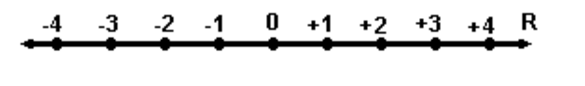
\includegraphics[width=3.9in,height=0.57in]{capitulos/conjuntos_numericos/media/image9.pdf}
	\end{Center}
\end{figure}

~~

Veja alguns exemplos de intervalos em  \( \mathbb{R} \) e suas respectivas representações na reta numerada:

\begin{figure}[H]
	\begin{Center}
		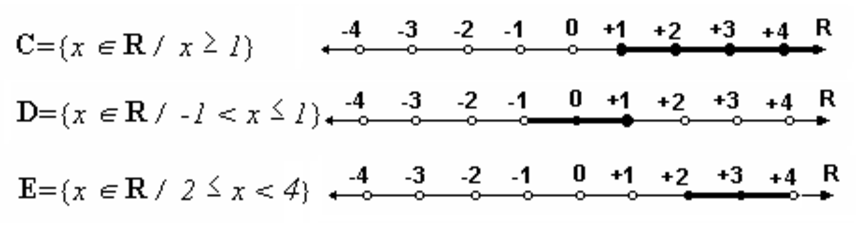
\includegraphics[width=5.72in,height=1.53in]{capitulos/conjuntos_numericos/media/image10.pdf}
	\end{Center}
\end{figure}

~~

Os conjuntos também podem ser representados usando parêntesis para \textit{intervalos abertos, por exemplo:}

(a,b) significa $ \{ $ \textit{ x \( \in \mathbb{R} \)  / a < x < b$ \} $ }

e com colchetes para \textit{intervalos fechados, por exemplo:}

[a,b] significa =$ \{ $ \textit{ x \( \in \mathbb{R} \)  / a$\leq$  x $\leq$  b$ \} $ .}

\begin{caixa}
	\begin{tdefinicao}

	Seja \textit{b um número real,~ m e n~números inteiros positivos.  Então,}

	\quad   \( b^{\frac{m}{n}}=\sqrt[n]{b^{m}} \) { .}
	\end{tdefinicao}
\end{caixa}
\textbf{Exemplo: \( ~~\sqrt[3]{3^{2}}=3^{\frac{2}{3}} \) ~ \qedsymbol{}}

\subsection{Propriedades dos radicais}

Sejam \textit{a e b números reais; m,n e p números inteiros positivos maiores do que 1.}

\textbf{P1)  \( \sqrt[n]{a \cdot b}=\sqrt[n]{a} \cdot \sqrt[n]{b} \) }

\textbf{P2)  \( \sqrt[n]{\frac{a}{b}}=\frac{\sqrt[n]{a}}{\sqrt[n]{b}} \) ~~para  \textit{b $ \neq $ ~ 0.}}

\textbf{P3)  \( \sqrt[n]{\sqrt[m]{b}}=\sqrt[nm]{b} \) }

\textbf{P4)  \(  \left( \sqrt[n]{b^{m}} \right) ^{p}=\sqrt[n]{a^{mp}} \) }

\textbf{P5) Para b $ \geq $ ~0    \( \sqrt[n]{b^{n}}=b . \) }

\textbf{P6)~Para~b~<~0       \( \sqrt[n]{b^{n}}= \left\{ \begin{matrix}
 \vert b \vert \textrm{ se n é par}\\
-b \textrm{ se n é ímpar} \\
\end{matrix} \right\}
 ~ \) }

\textbf{Exemplos: Simplifique os radicais:}

\begin{enumerate}
	\item  \( \sqrt[3]{81} \)  . Para simplificar esse radical vamos utilizar as propriedades P1 e P5.

 \[ \sqrt[3]{81}=\sqrt[3]{3^{4}}=\sqrt[3]{3^{3} \cdot 3}=3 \cdot \sqrt[3]{3} \] 

	\item  \( \sqrt[]{27y^{9}} \) ~~ se y > 0. Para simplificar esse radical vamos utilizar as propriedades P1 e P5.
\end{enumerate}

\quad  \( \sqrt[]{27y^{9}}=\sqrt[]{3  \cdot 3^{2} \cdot y^{8} \cdot y}=3y^{4}\sqrt[]{\text{3 y}} \) ~ \qedsymbol{}

\subsection{Racionalização de denominadores}

O denominador de algumas frações podem ter radicais. Nesse caso podemos usar a propriedade P5 para racionalizar (tornar racional) o denominador. 

\begin{texemplo}
	
Racionalize o denominador da fração~~   \( \frac{1}{\sqrt[]{3}}. \)

\textbf{Solução: Multiplicando-se a fração dada por 1, escrito na forma  \( \frac{\sqrt[]{3}}{\sqrt[]{3}}. \) ~~ não a alteramos. Então,  \( \frac{1}{\sqrt[]{3}} \cdot \frac{\sqrt[]{3}}{\sqrt[]{3}}=\frac{\sqrt[]{3}}{3} \) ~ \qedsymbol{}}
\end{texemplo}
\subsection{Operações com radicais}

\subsubsection{Adição e subtração}

Só é possível adicionar ou subtrair radicais semelhantes (\textit{índices e radicandos idênticos). }

\textbf{Exemplos:}

\begin{enumerate}
	\item  \( \sqrt[]{2}+3\sqrt[]{2}-5\sqrt[]{2}=-\sqrt[]{2} \) 

	\item  \( \sqrt[]{3}-2\sqrt[]{27}-\frac{\sqrt[]{12}}{2}.~ \)  Nesse caso, os radicais não são semelhantes. Porém,

 \( \sqrt[]{27}=3\sqrt[]{3} \) ~~e   \( \frac{\sqrt[]{12}}{2}=\frac{2\sqrt[]{3}}{2}=\sqrt[]{3} \) ~~ (usando as propriedades \textbf{P1 e P5). Substituindo estas igualdades na expressão dada, temos:}

 \( \sqrt[]{3}-3\sqrt[]{3}-\sqrt[]{3}=-3\sqrt[]{3}~ \) .
\end{enumerate}
	\subsubsection{Multiplicação e divisão de radicais}

As propriedades \textbf{P1 e P2 resolvem as operações de multiplicação e divisão, respectivamente, para radicais de mesmo índice. }

\textbf{Exemplos:}

\begin{enumerate}
	\item  \( \sqrt[]{2} \cdot \sqrt[]{5}=\sqrt[]{10} \) ~ . Foi usada a propriedade P1.

	\item  \( \sqrt[]{6}\text{~ : }\sqrt[]{2}=\sqrt[]{3} \) ~~~ Foi usada a propriedade P2.

	\item  \( \sqrt[]{3} \cdot \sqrt[4]{2}= \) 

Como o MMC(2,4)=4,~vamos transformar os radicais equivalentes com índice  4 e usar a propriedade P1.

 \[ \sqrt[2 \cdot 2]{3^{1 \cdot 2}} \cdot \sqrt[4]{2}=\sqrt[4]{3^{2}} \cdot \sqrt[4]{2}=\sqrt[4]{18} \] 

	\item  \( \sqrt[4]{2} \cdot \sqrt[6]{3}= \) 

Como o MMC(4,6)=12,~vamos transformar os radicais equivalentes com índice  12 e usar a propriedade P1.

 \[ \sqrt[4 \cdot 3]{2^{1 \cdot 3}} \cdot \sqrt[6 \cdot 2]{3^{1 \cdot 2}}=\sqrt[12]{8} \cdot \sqrt[12]{9}=\sqrt[12]{72} \] 

	\item  \( \sqrt[4]{2} \cdot \sqrt[6]{2}= \) 
\end{enumerate}

Como o MMC(4,6)=12,~vamos transformar os radicais equivalentes com índice  12 e usar a propriedade P1..

 \[ \sqrt[4 \cdot 3]{2^{1 \cdot 3}} \cdot \sqrt[6 \cdot 2]{2^{1 \cdot 2}}=\sqrt[12]{2^{5}}= \] 

Nesse caso (bases dos radicandos iguais) poderíamos usar a Def. 1.4.2 e resolver como multiplicação de potências de mesmas bases.

 \( \sqrt[4]{2} \cdot \sqrt[6]{2}=2^{\frac{1}{4}} \cdot 2^{\frac{1}{6}}=2^{\frac{5}{12}}=\sqrt[12]{2^{5}}~~~~~ \) \qedsymbol{}

\begin{exercicios}
	
	\exitem{} Calcule as raízes:

\begin{multicols}{6}
	
	a) \( \sqrt[3]{27} \)
	
	b)  \( \sqrt[3]{\frac{8}{27}} \)
	
	c)  \( \sqrt[3]{64} \)
	
	d)  \( \sqrt[5]{32} \)
	
	e)  \( \frac{\sqrt[]{64}}{\sqrt[4]{16}} \)
	
	f)  \( \sqrt[4]{\frac{625}{81}} \) 
\end{multicols}

	\exitem{} Os radicais do Ex.5.1 são números racionais ou irracionais?

	\exitem{} Simplifique os radicais:
	\begin{multicols}{6}

		 a) \(\sqrt[]{8} \)
		 
		 b)  \( \sqrt[]{12} \)
		 
		 c)  \( \sqrt[3]{24} \)
		 
		 d)  \( \sqrt[4]{32} \) 
		 
		 e)  \( \sqrt[]{\frac{12}{45}} \)
		 
		 f)  \( \sqrt[3]{\frac{16}{125}} \)
	\end{multicols}
	\exitem{} Os radicais do Ex 5.3 são números racionais ou irracionais?

	\exitem{} Coloque os coeficientes no radicando:
	\begin{multicols}{6}

	a) \( 2 \sqrt[]{3} \)
	
	b)  \( 3 \sqrt[3]{2} \)
	
	c)  \( 7 \sqrt[]{2} \)
	
	d)  \( \frac{1}{2}\sqrt[3]{4} \)
	
	e)  \( 3~ \cdot   \sqrt[]{\frac{1}{2}} \)
	
	f)  \( 5~ \cdot   \sqrt[]{\frac{3}{4}} \) 
	\end{multicols}
	\exitem{} Resolva as operações com os radicais:
	\begin{multicols}{4}
		a)  \( 3 \sqrt[]{3}+5\sqrt[]{3}-\sqrt[]{3} \) 
		
		b)  \( \sqrt[]{\frac{1}{2}}-~3  \sqrt[]{\frac{1}{2}} \)
		
		c)  \( \sqrt[]{5}  \cdot  \sqrt[3]{2} \)
		
		d)  \( \sqrt[]{3}  \cdot  \sqrt[]{5} \cdot \sqrt[]{\frac{1}{2}} \)
		
		e)  \( \sqrt[3]{\frac{3}{4}} \cdot 3~ \sqrt[3]{\frac{1}{2}} \)
		
		f)  \( ~7 \sqrt[]{5}  \cdot  3 \sqrt[]{2} \)
		
		g)  \( \sqrt[]{10}~:~\sqrt[]{2} \)
		
		h)  \( \sqrt[]{10}\text{~ : }\sqrt[]{\frac{1}{2}} \) 
\end{multicols}
	\exitem{} Resolva os produtos:

\begin{multicols}{2}
	a) \( 2~ \left( \sqrt[]{5}+3\sqrt[]{5} \right)  \)
	
	b)  \( \sqrt[]{2}~ \left( \sqrt[]{3}+\sqrt[]{5} \right)  \)
	
	c)  \( \sqrt[]{6}~ \left( \sqrt[]{32}-\sqrt[]{3} \right)  \)
	
	d)  \(  \left( 2+\sqrt[]{2} \right)  \cdot  \left( 2-\sqrt[]{2} \right)  \)
	
	e)~  \(  \left( 3-\sqrt[]{5} \right) ^{2} \)
	
	f)  \(  \left( \sqrt[]{7}-2\sqrt[]{3} \right)  \cdot  \left( \sqrt[]{7}+2\sqrt[]{3} \right)  \)
\end{multicols}

	\exitem{} Racionalize os denominadores:

\begin{multicols}{5}

	a) \( \frac{1}{\sqrt[]{3}} \)
	
	b)  \( \frac{3}{\sqrt[]{2}} \)
	
	c)  \( \frac{7}{\sqrt[]{5}} \)
	
	d)  \( \frac{3}{2+\sqrt[]{3}} \)
	
	e)  \( \frac{1}{\sqrt[]{2}-\sqrt[]{3}} \)
	
	f)  \( \frac{35}{\sqrt[]{3}-5} \)
\end{multicols}

\exitem{} Verifique~se~~~   \( \frac{-3}{2}=\frac{3}{-2}=-\frac{3}{2~} \) .

\exitem{} Escreva o respectivo conjunto numérico a que pertence cada um dos seguintes números:  0; $-$ 1; $-$ 34;  \( \sqrt[3]{8} \) ; 0,454545...; 212; $-$ 46;  \( \sqrt[3]{2} \) ; 12,1829421; 2,99999... e 3,76.

\exitem{} Explique porque \textit{-5 é um número inteiro e também é um número racional.}

\exitem{} Explique porque \textit{$-$ 15 é um número racional e também é um número inteiro.}

\exitem{} Escreva os números abaixo em forma de fração:
\begin{multicols}{3}
	
a) \textit{0,3}=

b) \textit{0,55555.}..=

c) \textit{1,32}= 

d) \textit{0,212121}...=

e) \textit{1,3333..}.=

f) \textit{3,434343}...=
\end{multicols}

	\exitem{}  Explique porque \textit{0,77777...} é um número racional.

	\exitem{}  Explique porque ~ $ \pi $  = 3,1415927... é um número irracional.

	\exitem{}  Explique porque  \( \frac{4}{6}=\frac{2}{3} \)  ~~ 

	\exitem{}  Indique o conjunto de números adequado para cada variável:
	\begin{enumerate}[label=\alph*)]
    \item Tempo de vida de um pé de milho.

    \item Altura de um pé de soja.

    \item Número de vacas de uma propriedade.

    \item Produção leiteira.

    \item Teor de água do solo.

    \item Massa de solo.

    \item Massa de um suíno.

    \item Volume de água de uma amostra de solo.

    \item Número de frangos em um aviário.

    \item Diagonal de um quadrado.
\end{enumerate}
	\exitem{} Escreva os intervalos por compreensão:
	\begin{multicols}{2}
	
		a) \textbf{\textit{A}}\textit{=$ \{ $ 1,2,3,4,5$ \} $ }.
		
		b) \textbf{\textit{B}}\textit{=$ \{ $ -3,-2,-1,0,1,2$ \} $ }.

		c) os números reais maiores ou iguais a -3.
		
		d) os números reais entre -3 e 5.

		e) os números reais menores que 3 e maiores que 5.
	\end{multicols}

	\exitem{}  Represente os intervalos na reta real:
	\begin{multicols}{2}
	a) $P= \{ x \in {\mathbb{R} }/ -  1 < x < 3 \} $
	 
	b) $K= \{ x \in \mathbb{R} / - 2 \leq x < 3/4 \} $ 

	c) $C= \{ x \in \mathbb{R} /0, 5 < x \leq  5 \} $
	
	d) $D= \{ x \in \mathbb{R} / \frac{2}{3} < x < \frac{4}{3} \} $ 

	e) $F= \{ x \in \mathbb{R}/ - 3 > x \} $
	
	f) $H = \{ x \in \mathbb{R}/ x > 0, 5$ 

	g) $B= \{ x \in \mathbb{R} / - 2 \leq x < 1 \} $
	
	h) $J= \{ x \in \mathbb{R} / x < +3 \} $ 
\end{multicols}
	\exitem{} O número \(  \left( \sqrt[]{7+4\sqrt[]{3}}+\sqrt[]{7-4\sqrt[]{3}} \right) ^{2} \) ~~~ é racional ou irracional?
\end{exercicios}

\section{RESPOSTAS DOS EXERCÍCIOS PROPOSTOS}

\begin{respostas}{2}
	\ansitem{}
	\begin{multicols}{3}
		
	a) A=$ \{ $ 6,7,8,9,10,...$ \} $
	
	b) B=$ \{ $ 2,3,4,5,6,7,8,9$ \} $
	
	c) C=$ \{ $ 0,1,2,3,4,5,6$ \} $ 

	d) D=$ \{ $ 2,3,4,5,6,7$ \} $
	
	e) E=$ \{ $ 3,4,5$ \} $ 
	
	f) F=$ \{ $ 0,1,6,7,8,9,10,...$ \} $ 
	\end{multicols}
	\ansitem{}
a) 
\begin{figure}[H]
	\begin{Center}
		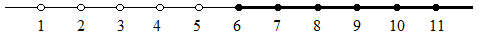
\includegraphics[width=1.46in,height=0.8in]{capitulos/conjuntos_numericos/media/image11.png}
	\end{Center}
\end{figure}
~~
b) 
\begin{figure}[H]
	\begin{Center}
		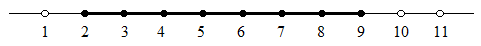
\includegraphics[width=4.4in,height=0.48in]{capitulos/conjuntos_numericos/media/image12.png}
	\end{Center}
\end{figure}
~~
c)
\begin{figure}[H]
	\begin{Center}
		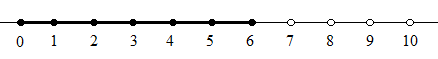
\includegraphics[width=4.56in,height=0.61in]{capitulos/conjuntos_numericos/media/image13.png}
	\end{Center}
\end{figure}
~~
d)
\begin{figure}[H]
	\begin{Center}
		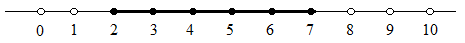
\includegraphics[width=4.84in,height=0.45in]{capitulos/conjuntos_numericos/media/image14.png}
	\end{Center}
\end{figure}
~~
e)
\begin{figure}[H]
	\begin{Center}
		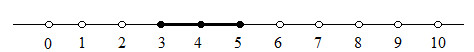
\includegraphics[width=4.94in,height=0.54in]{capitulos/conjuntos_numericos/media/image15.png}
	\end{Center}
\end{figure}
~~
f)
\begin{figure}[H]
	\begin{Center}
		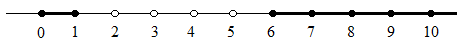
\includegraphics[width=4.83in,height=0.5in]{capitulos/conjuntos_numericos/media/image16.png}
	\end{Center}
\end{figure}
~~
	\ansitem{} a) Sim, b) Sim, c) Sim, mas em geral, é um número fracionário d) Sim e) Sim, mas em geral, é um número fracionário.

    \ansitem{} Não.

	\ansitem{} Não existe.

	\ansitem{} a)Sim, b) Não, c) Sim, e d) Não.

\end{respostas}

\begin{respostas}{3}
	\ansitem{} a) 3.~~~~ b) -25.~~ ~ c) -9.~~~~ d) -1.~~~~~ e) -2.~~~~ f) 35.~~~~~ g) 0.~~ ~ h) -22.~ ~  i) -8. ~~~~ j) 10.

	\ansitem{} R$\$$  -850,00.

	\ansitem{} a) 50 – 30 = 20.\quad b) 100 – 40 = 60.  \quad c) -100 + 50 = -50.\quad d) -200 – 70 = -270.

	\ansitem{} + 21ºC.

	\ansitem{} – 10ºC.

	\ansitem{} 220m.

	\ansitem{} Sim, (–2).

	\ansitem{} \( 6/2=~3   \in \mathbb{Z};6/4 \notin  \mathbb{Z} \).  

\ansitem{} a)~16.~~~~~b)~-64.~~~ c)0.     d)~1.~~  ~~ e)~+25.~~~~f)~+16.~~~~g)-16.     h)-32.

\ansitem{}a) $ \pm $ ~3.~~~~b)~3.~~~~~~~c)~-3.~~~~d)~$ \pm $ ~2.~~~~e)~$ \pm $ ~2.~~~~ f)+2.      g)-2.       h)-4.
\end{respostas}

\begin{respostas}{4}
	\ansitem{} a) -1.\quad b) -11/10.~~~ \quad c) $\frac{1}{2}$.\quad  d)1. ~~~~~~ e)1/24.\quad f)1.

	\ansitem{} a)-1/2.\quad b)4/9.~~~~~~~ c)-13/2.\quad d)-1/5.~~~~~~~ e)30.\quad f)3/2.
\end{respostas}

\begin{respostas}{5}
	\ansitem{} a)3.\quad b)2/3.\quad \quad c)4.\quad d)2.\quad e)4.\quad f)5/3.

	\ansitem{}  Racionais.

	\ansitem{} a)  \( 2\sqrt[]{2} \) \quad b)  \( 2\sqrt[]{3} \) ~~~ \quad c)  \( 2\sqrt[3]{3} \) \quad \quad d)  \( 2\sqrt[4]{2} \) ~~~~~~~~~ e)  \( \frac{2\sqrt[]{3}}{3\sqrt[]{5}} \) \quad \quad f)  \( \frac{2\sqrt[3]{2}}{5} \) 

	\ansitem{}  Irracionais. 

	\ansitem{}  a)  \( \sqrt[]{12} \) \quad b)  \( \sqrt[3]{54} \) \quad \quad c)  \( \sqrt[]{98} \) \quad \quad d) \( ~\sqrt[3]{\frac{1}{2}} \) ~~~~~~~~~~ e)  \( \sqrt[]{\frac{9}{2}} \) ~~~~~~~~ f)  \( \sqrt[]{\frac{75}{4}} \) 

	\ansitem{} a)  \( 7\sqrt[]{3} \) \quad b)  \( -2\sqrt[]{\frac{1}{2}} \)  ~ ~~ c)  \( \sqrt[6]{500} \) \quad ~~~ d)  \( \sqrt[]{\frac{15}{2}} \) ~~~~ e)  \( 3\sqrt[3]{\frac{3}{8}} \) \quad f)  \( 21\sqrt[]{10} \) ~~~ g)  \( \sqrt[]{5} \) \quad h)  \( \sqrt[]{20} \) 

	\ansitem{}  a)  \( 8\sqrt[]{5} \) \quad b)  \( \sqrt[]{6}+\sqrt[]{10} \) ~~~  c)  \( 8\sqrt[]{3}-3\sqrt[]{2} \) \quad d)  \( 2 \) ~~~ \quad  e)  \( 14-6\sqrt[]{5} \) \quad ~~~~~ f)  \( -5 \) 

	\ansitem{} ~ a)  \( \frac{\sqrt[]{3}}{3} \) \quad b)  \( \frac{3\sqrt[]{2}}{2} \) ~~ ~ c)  \( \frac{7\sqrt[]{5}}{5} \) ~~~~~ d)  \( 6-3\sqrt[]{3} \) ~~~~ e)  \( -\sqrt[]{2}-\sqrt[]{3} \) \quad f)  \( \frac{-175-35\sqrt[]{3}}{22} \) 

	\ansitem{}São iguais.

	\ansitem{} Respectivamente:$\mathbb{N}, \mathbb{Z}, \mathbb{Z}, \mathbb{I}, \mathbb{Q}, \mathbb{N}, \mathbb{Z}, \mathbb{I}, \mathbb{Q}, \mathbb{Q}, \mathbb{Q}$.

	\ansitem{} Porque o conjunto dos números Inteiros ($\mathbb{Z}$) está contido no conjunto dos números Racionais ($\mathbb{Q}$).

	\ansitem{}  -15~é um número inteiro, mas também é racional, porque podemos escrevê-lo  na forma de fração: -30/2, por exemplo.

	\ansitem{} ~ a)  \( \frac{3}{10} \) \quad  b)  \( \frac{5}{9} \) ~~~~~~  c)  \( \frac{132}{100} \) \quad d)  \( \frac{7}{33} \) ~~~~~ ~ e)  \( \frac{4}{3} \) \quad \quad f)  \( \frac{340}{99} \) ~~ 

	\ansitem{}Porque é um número decimal periódico infinito.

	\ansitem{}Porque é um número decimal não periódico.

	\ansitem{} Devido~à equivalência de frações, pois   \( \frac{2}{3} \cdot \frac{2}{2}=\frac{4}{6} \).
	
	\ansitem{}
\begin{multicols}{10}
	
	a) \( \mathbb{Q} \)
	
	b) \( \mathbb{Q} \)
	
	c) \( \mathbb{N} \)
	
	d) \( \mathbb{Q} \)
	
	e) \( \mathbb{Q} \)
	
	f) \( \mathbb{Q} \)

	g) \( \mathbb{Q} \)
	
	h) \( \mathbb{Q} \)
	
	i) \( \mathbb{N} \)
	
	j) $\mathbb{R}$
\end{multicols}
	\ansitem{}
	a) \( A =  \{ x \in \mathbb{N}/ x < 6 \}  \) 

	b)  \( B =  \{ x \in \mathbb{Z}/ -4 < x < 3 \}  \) 

	c)  \( C =  \{ x \in \mathbb{R}\frac{}{}x \geq -3 \}  \) 

	d)  \( D =  \{ x \in \mathbb{R} / -3 < x < 5 \}  \) 

	e)  \( E =  \{ x \in \mathbb{R} / 3 > x> 5 \}  \) 

	\ansitem{}
a)

\begin{figure}[H]
	\begin{Center}
		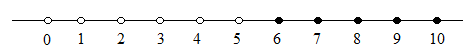
\includegraphics[width=3.92in,height=0.58in]{capitulos/conjuntos_numericos/media/image17.png}
	\end{Center}
\end{figure}

~~
 b)

\begin{figure}[H]
	\begin{Center}
		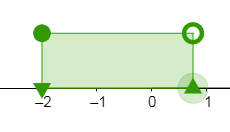
\includegraphics[width=3.83in,height=0.53in]{capitulos/conjuntos_numericos/media/image18.png}
	\end{Center}
\end{figure}

~~

 c)

\begin{figure}[H]
	\begin{Center}
		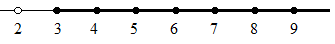
\includegraphics[width=3.49in,height=0.46in]{capitulos/conjuntos_numericos/media/image19.png}
	\end{Center}
\end{figure}

~~

d)

\begin{figure}[H]
	\begin{Center}
		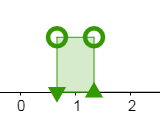
\includegraphics[width=4.17in,height=0.56in]{capitulos/conjuntos_numericos/media/image20.png}
	\end{Center}
\end{figure}

~~

 e)

\begin{figure}[H]
	\begin{Center}
		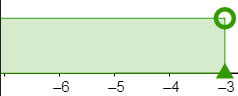
\includegraphics[width=4.38in,height=0.45in]{capitulos/conjuntos_numericos/media/image21.png}
	\end{Center}
\end{figure}

~~

 f)

\begin{figure}[H]
	\begin{Center}
		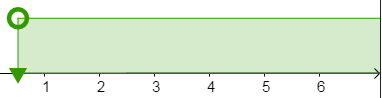
\includegraphics[width=4.38in,height=0.45in]{capitulos/conjuntos_numericos/media/image22.png}
	\end{Center}
\end{figure}

~~

 g)

\begin{figure}[H]
	\begin{Center}
		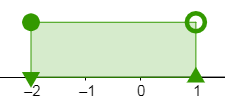
\includegraphics[width=4.38in,height=0.45in]{capitulos/conjuntos_numericos/media/image23.png}
	\end{Center}
\end{figure}

~~

 h)

\begin{figure}[H]
	\begin{Center}
		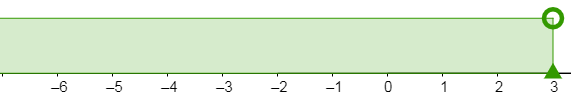
\includegraphics[width=4.38in,height=0.45in]{capitulos/conjuntos_numericos/media/image24.png}
	\end{Center}
\end{figure}

~~

\ansitem{} O número representado por este produto notável é racional (16).

\end{respostas}


\section{Grandezas Proporcionais}

\section{Expressões Algébricas}

\subsection{Expressões Algébricas}

A Matemática é uma linguagem e como tal, expressa alguma coisa. Ao calcular a área de um retângulo com \textit{3 cm} de comprimento e \textit{4 cm} de largura, escrevemos $3 \cdot 4$ (três vezes quatro) e estamos expressando a soma de $4 + 4 + 4$.  Tanto $3 \cdot 4$ como $4 + 4 + 4$ são expressões numéricas, cujo significado particular é o número de $cm^2$ do retângulo.

Para escrever de modo geral a área de qualquer quadrado de lado $x$, usamos $x^2$. Esta expressão com \textit{letras} e \textit{números}, chamamos de \textit{expressão algébrica}.

\vspace{5mm}

\settowidth\widest{\textbf{(a)}}
\stepcounter{exemplo}
\begin{description}[leftmargin=\dimexpr\widest+\labelsep\relax,labelindent=0pt,
    labelwidth=\widest]
\item[\textbf{Exemplo~\thesubsection.\theexemplo~-}]

\noindent O lado do quadrado pode ser expresso pela letra  x  e isso significa que o lado é variável, ou seja, pode assumir diferentes valores positivos.

\begin{figure}[h]
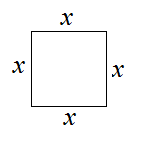
\includegraphics{capitulos/expressoes_algebricas/media/image2.png}
\centering
\end{figure}

\noindent Se \textit{$x = 2$ cm} o quadrado tem todos os lados iguais a \textit{2 cm} e é aproximadamente do tamanho de um ladrilho de revestimento de paredes.

\noindent Se \textit{$x = 2,2$ m}, o quadrado tem todos os lados iguais a $2,2$ \textit{m} e é aproximadamente do tamanho de banheiro.

\noindent Se \textit{$x = 1$ hm} (\textit{100m}), o quadrado tem todos os lados iguais a \textit{1 hm} e é aproximadamente do tamanho de uma quadra de cidade.

\noindent Devemos observar que o lado do quadrado expresso por $x$ é variável, ou seja, pode assumir diferentes valores.

\noindent Para cada valor de $x$ proposto acima, o perímetro (\textit{P}) de todos os quadrados, pode ser escrito com uma equação algébrica:

\begin{center}
\textit{P = 4x.}
\end{center}

\noindent Dizemos que $4x$ é a expressão algébrica do perímetro de qualquer quadrado de lado $x$. Nesse caso, o número $4$ é uma constante (coeficiente, parte numérica) e $x$ é a variável (parte literal) \qedsymbol

\noindent As expressões algébricas recebem nomes específicos em função do número de termos:

\setlength{\parskip}{.5em}
\noindent 1 termo = \textbf{monômios}. Exemplos: $7x^3$; $3m^2n^4$\par
\setlength{\parskip}{0em}
\noindent 2 termos = \textbf{binômios}. Exemplos:  $x+1$; $7x^3 -4x$; $4y - 3$; $x^2 - 1$\par
\noindent 3 termos = \textbf{trinômios}. Exemplos: $x^4 - x^3 + 3$; $x^2$- $2x$ + 3\par
\noindent Mais do que 3 termos = \textbf{polinômios}. Exemplo: $2x^4$ - $3x^3$ + $3x^2$ + 2.

\end{description}

\setlength{\parskip}{.5em}

\textbf{\textit{Definição}}: dois monômios são semelhantes se as partes literais forem idênticas.

\newpage

\stepcounter{exemplo}
\textbf{Exemplo~\thesubsection.\theexemplo~-}
\settowidth\widest{\textbf{(a)}}
\begin{description}[leftmargin=\dimexpr\widest+\labelsep\relax,labelindent=0pt,
    labelwidth=\widest]
\item
\begin{enumerate}[label=(\textbf{\alph*)}]
    \item Os monômios $7x^3$ e $3x^3$ são semelhantes, pois as partes literais são idênticas;
    
    \item Os monômios  $2ab^2$ e $2a^3b$ não são semelhantes, pois as partes literais são diferentes \qedsymbol
\end{enumerate}

\end{description}

\noindent\textbf{EXERCÍCIOS \thesubsection}

\settowidth\widest{\textbf{(a)}}

\begin{enumerate}[label=\thesubsection.\arabic*]

\exitem{Use variáveis para expressar o perímetro e a área de:}
\begin{enumerate}[label=(\textbf{\alph*)}]
\item Quadrados
\item Retângulos em que um lado é o dobro do outro
\item Retângulos em que a diferença dos lados é \textit{2 cm}
\item Retângulos em que um lado é \textit{5 cm} maior do outro
\end{enumerate}

\exitem{Determine a expressão algébrica do perímetro do retângulo}
\begin{figure}[h]
  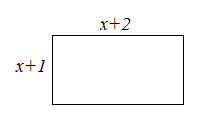
\includegraphics{capitulos/expressoes_algebricas/media/image3.png}
  \centering
\end{figure}

\exitem{Determine a expressão algébrica do perímetro da figura:}
\begin{figure}[h]
  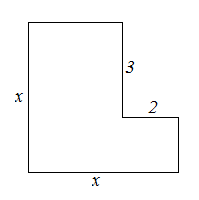
\includegraphics{capitulos/expressoes_algebricas/media/image4.png}
  \centering
\end{figure}

\exitem{Determine o perímetro da figura do \hyperref[ex:{{3.1.3}}]{\textbf Ex 3.1.3} para $x = 4$.}

\exitem{O valor de $x$ poderia ser $1$ na figura do \hyperref[ex:{{3.1.3}}]{\textbf Ex 3.1.3} ?}

\exitem{Calcule o valor numérico das expressões com os respectivos valores das variáveis:}

\begin{multicols}{2}\large
a) $7x^3 + x^2 - 3x + 1$ para $x = -2$\\
b) $ - x^4 + 5x - \frac{1}{3}$ para $x = - 1$\\
c) $\frac{x+1}{x^2-2}$ para $x = 2$\\
d) $\frac{x+1}{x^2-x+1}$ para $x=\frac{1}{2}$
\end{multicols}\normalsize

\end{enumerate}

\subsection{Operações com monômios e polinômios}

\begin{center}\fbox{\begin{minipage}{.9\textwidth}\begin{center}

    \textbf{Adição e subtração de monômios e polinômios}
    
    \vspace{5mm}
    
    Só é possível adicionar ou subtrair monômios semelhantes.\\
    
    \vspace{5mm}
    
    Para adicionar ou subtrair monômios, soma-se ou subtrai-se os coeficientes e mantem-se a parte literal.\\
    
    \vspace{5mm}
    
    Para adicionar/subtrair polinômios, soma-se ou subtrai-se os monômios semelhantes.\\
    
\end{center}\end{minipage}}\end{center}

\stepcounter{exemplo}
\textbf{Exemplo~\thesubsection.\theexemplo~-}
\settowidth\widest{\textbf{(a)}}
\begin{description}[leftmargin=\dimexpr\widest+\labelsep\relax,labelindent=0pt,
    labelwidth=\widest]
\item[]

\begin{enumerate}[label=(\alph*)]
    \item $3x^2 + 5x^2 - 2x^2 = (3+5-2)x^2 = 6x^2$
    \item $5y - 7x - 8y + 6x = (5-8)y + (-7+6)x = -3y - x$
    \item $(x^2 + 5x -3) - ( 2x^2 + 2x -8) = -x^2 + 3x + 5$
\end{enumerate}

\end{description}

\begin{center}\fbox{\begin{minipage}{.85\textwidth}\begin{center}

    \textbf{Multiplicação e divisão de monômios}
    
    \vspace{5mm}
    
    Multiplica-se ou divide-se os coeficientes e usa-se a propriedade da multiplicação/divisão de potências de mesma base para multiplicar a parte literal.
    
\end{center}\end{minipage}}\end{center}

\stepcounter{exemplo}
\textbf{Exemplo~\thesubsection.\theexemplo~-}
\settowidth\widest{\textbf{(a)}}
\begin{description}[leftmargin=\dimexpr\widest+\labelsep\relax,labelindent=0pt,
    labelwidth=\widest]
\item[]

\begin{enumerate}[label=(\alph*)]
    \item $(-3x^2 ) \cdot (7x^2) = -21x^4$
    \item $(25x^4 y^2) \div (5x^2 y) = 5x^2y$
    \item $(10x^2) \div (2x) = 5x$
    \item $(12x^3 + 6x^2 - 5x) \div (-2x) = -6x^2 - 3x + \frac{5}{2}$.   

\end{enumerate}
\end{description}

\stepcounter{exemplo}
\textbf{Exemplo~\thesubsection.\theexemplo~-} Multiplique $12 \cdot 15$ \label{ex:3.2.3}

\begin{description}
\item[Solução:]
Vamos escrever $12 = 10 + 2$ e $14 = 10 + 4$. Para multiplicar usamos a propriedade distributiva da multiplicação em relação à adição:

$(10 + 2) \cdot  (10 + 4) = 10 \cdot 10 + 10 \cdot 4 + 2 \cdot 10 + 2 \cdot 4 = 100 + 40 + 20 + 8 = 168$.

Ou, na forma de algoritmo:

\hspace{7mm} 1d + 4u

\hspace{7mm} 10 + 2

\hspace{7mm} ---------

\hspace{7mm} 2d    + 8u

\hspace{-1mm} 1c  + 4d

            ---------------

            1c + 6d + 8u        = 168 u $\qedsymbol$


\end{description}

\stepcounter{exemplo}
\noindent\textbf{Exemplo \thesubsection.\theexemplo~-} Multiplique os polinômios: $(x^3 + 6x^2 - 5x) \cdot (x - 2)$

\begin{description}
\item[\textbf{Solução:}]
A multiplicação de dois polinômios segue o mesmo algoritmo da multiplicação de dois números decompostos como soma, como no \hyperref[ex:3.2.3]{\textbf{Ex 3.2.3}}

\hspace{8mm}$x^3 + 6x^2 - 5x$
                
\hspace{23mm}x – 2
		      			 
\hspace{4mm}------------------------
				
\hspace{4mm} $-2x^3 -12x^2  + 10x$
       		       	          
$x^4 +6x^3 -5x^2 $ 
		                
---------------------------
			
$x^4  +  4x^3  -17x^2  + 10x$ $\qedsymbol$
\end{description}


\stepcounter{exemplo}
\textbf{Exemplo \thesubsection.\theexemplo~-} Divida os polinômios: $(x^3 + 6x^2 - 5x) \div (x - 2)$.

\begin{description}
\item[\textbf{Solução:}]
A divisão de polinômios é semelhante ao algoritmo da divisão de dois números inteiros.

\[
\begin{array}{rl}
x^3 + 6x^2 - 5x & \myrule{x-2} \\
\cline{2-2}
-x^3 + 2x^2~~~~~~~~ & x^2  + 8x \\
------\\
+8x^2-5x\\
-8x^2+16x\\
-----\\
+11x
\end{array}
\]
A divisão dos polinômios dá $x^2  + 8x$ e o resto é $+11x$ $\qedsymbol$

\end{description}

\noindent\textbf{EXERCÍCIOS \thesubsection}

\begin{enumerate}[label=\thesubsection.\arabic*]

\exitem{Explique porque podemos cancelar $a$ em $\frac{a \cdot{} b}{a}$ e não podemos em $\frac{a+b}{a}$.}

\exitem{Verifique se as igualdades são verdadeiras (justifique sua resposta):}
\begin{multicols}{2}

\begin{enumerate}[label=\alph*)]

\item $a^2  + a^3  = a5$

\item $x^3  \cdot  x^3 = x^6$

\item $y^3 : y^3 = 1$

\item $2m^2 - 3m^2 = -m^2$

\item $x^3 \cdot x^3 = 2x^6$

\item $10y^3 : 2y^2 = 5y$

\end{enumerate}

\end{multicols}

\exitem{Resolva as operações com as expressões algébricas:}

\begin{multicols}{2}

\begin{enumerate}[label=\alph*)]
    \item $3x^2 + \frac{1}{3}x^2 - 2x^2$
    
    \item $ab^2 - \frac{1}{2}ab^2 + \frac{1}{4}ab^2$
    
    \item $y^3 - \frac{3}{4}y^3 + 2y^3$
    
    \item $x(xy+2x+3y)$
    
    \item $(x-3)(x^2-\frac{1}{3}x+3$
    
    \item $a^2b \cdot ab^3 \cdot a^3b$
    
    \item $(y^2-\frac{1}{5} \cdot (5y-2)$
    
    \item $7a^3b^2x^2 : 14a^2bx$
    
    \item $(2x^3+5x^2+2x) : (x+\frac{1}{2}$
    
    \item $\frac{1}{2}m^3n^2 : \frac{1}{4}m^2n+mn$
\end{enumerate}

\end{multicols}

\exitem{Dados os polinômios $A = 2x+1$; $B = x-3$ e $C = 2x^2+5x+2$, resolva:}

\begin{multicols}{4}

\begin{enumerate}[label=\alph*)]
    \item $A+B$
    
    \item $B+C-A$
    
    \item $A \cdot B$
    
    \item $A \cdot C$
    
    \item $C - x \cdot A$
    
    \item $C:A$
    
    \item $C:B$
    
    \item $A \cdot B-C$
\end{enumerate}

\end{multicols}

\exitem{Um lado de um retângulo é expresso por $x +3$ e outro por $2x$:}

\begin{enumerate}[label=\alph*)]
\item Determine a expressão algébrica do perímetro.

\item Determine a expressão algébrica da área.

\item Para que valor de $x$ o perímetro é $18cm$?

\item Se a área é $56cm^2$, qual é o valor de $x$?

\item Qual é o valor de $x$ para que os lados sejam iguais?
\end{enumerate}

\exitem{A área de um retângulo é expressa por $x^2+2x-3$ e um dos lados por $x-1$. Determine a expressão algébrica do outro lado.}

\exitem{O lado de um cubo é expresso por $x+1$. Determine a expressão algébrica:}

\begin{enumerate}[label=\alph*)]
    \item Do volume
    \item Da área de uma face
    \item Da área superficial
\end{enumerate}

\exitem{Com base na figura, determine as expressões algébricas do perímetro e da área.}

\begin{figure}[H]
~~~~~~~
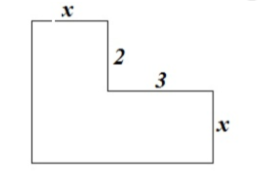
\includegraphics[scale=.8]{capitulos/expressoes_algebricas/media/image5.png}
\end{figure}

\exitem{O lado de um quadrado é expresso por $x+3$:}

\begin{enumerate}[label=\alph*)]
\item Determine a expressão algébrica da área.

\item Calcule a área para $x = 1$.

\item $x$ pode ser zero?

\item Qual o valor de $x$ para que a área seja nula.

\end{enumerate}

\exitem{Calcule os valores da área do quadrado do \hyperref[ex:{{3.2.9}}]{\textbf{Ex 3.2.9}} para $x = {-3,-2,-1,0,1,2,3}$}

\end{enumerate}

\subsection{Produtos Notáveis}

Produtos notáveis são produtos especiais de polinômios. São chamados “notáveis” porque aparecem seguidamente em problemas de Matemática.

~~

\textbf{Quadrado da soma de dois termos}: $(a+b)^2 = a^2 + 2ab + b^2$

~~

\textbf{Quadrado da diferença de dois termos}: $(a - b)^2 = a^2 - 2ab + b^2$

~~

\textbf{Produto da soma pela diferença}: $(a + b) \cdot (a - b) = a^2 - b^2$

~~

\textbf{Cubo da soma de dois termos}: $(a + b)^3 = a^3 + 3a^2b + 3ab^2 + b^3$

~~

\textbf{Cubo da diferença de dois termos}: $(a - b)^3 = a^3 - 3a^2b + 3ab^2 - b^3$

~~

\noindent\textbf{EXERCÍCIOS \thesubsection}

\begin{enumerate}[label=\thesubsection.\alph*)]
\begin{multicols}{3}
    \exitem{$(x+5)^2$}
    
    \exitem{$(2x-3)^2$}
    
    \exitem{$(x+\frac{1}{2})^2$}
    
    \exitem{$(3-x)^2$}
    
    \exitem{$(\frac{1}{2}x+2)^2$}
    
    \exitem{$(x+1)^3$}
    
    \exitem{$(2x-5)^3$}
    
    \exitem{$(x-3)(x+3)$}
    
    \exitem{$(m+3n)(m+3n)$}
    
    \exitem{$(x+\frac{1}{2})(x-\frac{1}{2})$}
    
    \exitem{$(x+1)(x+2)$}
    
    \exitem{$(x-1)(x+3)$}
    
    \exitem{$(2a-b)(2a+b)$}
    
    \exitem{$(a+b+1)^2$}
    
    \exitem{$(x+\frac{1}{4})(x+2)$}
\end{multicols}
\end{enumerate}

\subsection{Fatoração}

\begin{center}\fbox{\begin{minipage}{.85\textwidth}\begin{center}

    \textit{\textbf{Fatores} são os termos de uma multiplicação e \textbf{fatorar} é transformar um número ou expressão algébrica em um produto de fatores.}
    
\end{center}\end{minipage}}\end{center}


\begin{description}
\item [Exemplos:] ~
\begin{enumerate}[label=\alph*)]
\item O número 12 fatorado é $3 \cdot 4$ , onde 3 e 4 são fatores.

\item Podemos decompor números em fatores primos, por exemplo: $24 = 2 \cdot2 \cdot 2 \cdot 3$. Os números 2 e 3, nesse caso são fatores, onde o fator 2 aparece três vezes.

\item Na expressão $3x^2a^3$, 3, $x^2$  e $a^3$ são fatores.
\end{enumerate}
\end{description}

\begin{description}
\item [Fatoração com Fator Comum:]~

Algumas expressões algébricas têm \textit{fatores comuns} (fatores que estão presentes em mais de uma expressão algébrica) que se pode colocar em evidência (colocar em separado, na forma de fatores). Vejamos os exemplos:
\begin{enumerate}[label=\alph*)]
\begin{multicols}{2}
\item $3x + 6y = \colorbox{gray}{3}x + 2 \cdot \colorbox{gray}{3}y = 3 \cdot (x+2y)$.

Observemos que o 3 é fator comum aos dois monômios.
\end{multicols}

\begin{multicols}{2}
\item $4ab^3 - 2a^3b + 10ab^4 = 2ab \cdot (2b^2 - a^2 + 5b^3)$.

Observemos  que o 2ab é fator comum aos três monômios
\end{multicols}

\begin{multicols}{2}
\item $2an + 2bn - am - bm$.

\textbf{(Fatoração por agrupamento)}
\end{multicols}

Nos dois primeiros termos o fator comum é $2n$ e nos dois últimos o fator comum é $-m$.

~~

$2an + 2bn - am - bm = 2n(a+b) - m(a+b)$

~~

A expressão resultante tem mais um fator comum: $(a+b)$. Então:

~~

$2an + 2bn - am - bm = (a+b)(2n-m)$. 
\end{enumerate}
\end{description}

\begin{description}
\item [Fatoração do Trinômio Quadrado Perfeito (TQP):]~

Um trinômio é \textit{quadrado perfeito (TQP)} se foi originado pelo quadrado da soma ou subtração de dois termos.

\begin{multicols}{2}
$a^2 + 2ab + b^2 = (a + b)^2$

(\textit{Quadrado da soma de dois termos})
\end{multicols}

\begin{multicols}{2}
$a^2 - 2ab + b^2 = (a - b)^2$

(\textit{Quadrado da diferença de dois termos})
\end{multicols}

Observemos que o trinômio foi \textit{transformado (fatorado)} em um produto onde os fatores são $(a \pm b)$. Chamando $a$ de \textit{“primeiro termo do binômio”} e $b$ de \textit{“segundo termo do binômio”}, dizemos que o trinômio $a^2 + 2ab + b^2$ é o quadrado do primeiro, mais duas vezes o primeiro vezes o segundo mais o quadrado do segundo.

\end{description}

\begin{description}
\item [Fatoração da Diferença de dois quadrados:]~

\begin{multicols}{2}
$a^2 - b^2 = (a+b) \cdot (a - b)$

(\textit{Produto da soma pela diferença de dois termos})
\end{multicols}
\end{description}

\stepcounter{exemplo}
\noindent\textbf{Exemplo \thesubsection.\theexemplo~-} Verifique se $x^2 + 2x + 1$ é um TQP.

\begin{description}
\item [Solução:] Se o trinômio dado é um TQP então o primeiro termo do binômio $(a+b)$ deve ser $a = \sqrt{x^2} = x$  ; o segundo termo do binômio $(a+b)$ deve ser $b = \sqrt{1} = 1$.

\textbf{Teste do segundo termo do trinômio:}  $2 \cdot a \cdot b = 2 \cdot x \cdot 1 = 2x$  deve ser igual ao \textit{segundo termo do trinômio}. O que de fato ocorre, neste caso. Assim,

\begin{center} $(x + 1)^2 = x^2 + 2x + 1$. \end{center}

Portanto, o polinômio dado é um TQP \qedsymbol{}

\end{description}

\stepcounter{exemplo}
\noindent\textbf{Exemplo \thesubsection.\theexemplo~-} Verifique se $x^2 + 2x + 4$ é um TQP.

\begin{description}
\item [Solução:] Se o trinômio dado é um TQP então o primeiro termo deve ser $a = \sqrt{x^2} = x$ e o segundo termo $b = \sqrt{4} = 2$.

\textbf{Teste do segundo termo do trinômio:}  $2 \cdot a \cdot b = 2 \cdot x \cdot 2 = 4x$, que é diferente de 2x. Portanto, o trinômio dado não é um TQP \qedsymbol{}

\end{description}

\stepcounter{exemplo}
\noindent\textbf{Exemplo \thesubsection.\theexemplo~-} Complete o trinômio $x^2 - 4x + 1 = 0$, de modo que obtenha-se um TQP.

\begin{description}
\item [Solução:] Para se obter um TQP na identidade dada, o primeiro termo do binômio $(a+b)$ deve ser $a=\sqrt{x^2}=x$. O segundo termo "$b$" pode ser obtido, sabendo que

\begin{multicols}{2}
\item ~~~~~~~~$2 \cdot x \cdot b = -4x$

\item \textit{(duas vezes o primeiro termo, vezes o segundo termo é igual ao segundo termo do trinômio)}
\end{multicols}

Assim, $b = -2$ e o TQP é $(x-2)^2 = x^2 - 4x + 4$.

Para obter o TQP no lado esquerdo da identidade dada, basta adicionar (+3) em ambos os lados:

~~

$x^2 - 4x +1 +(+3) = 0 +(+3)$

~

$x^2 -4x + 4  = 3$ \qedsymbol{}

\end{description}

\textbf{EXERCÍCIOS \thesubsection}

\begin{enumerate}[label=\thesubsection.\arabic*]

\exitem{Fatore as expressões algébricas:}

\begin{multicols}{2}
\begin{enumerate}[label=\alph*)]
\item $x^2-x$

\item $a^3b^2-ab+ab^2$

\item $9x^2-12x+4$

\item $9+6x+x^2$

\item $x^2+x+\frac{1}{4}$

\item $x^2-25$

\item $16x^2-\frac{4}{9}$

\item $ax+bx+ay+by$

\item $6+3x+2y+xy$

\item $x^3+1$
\end{enumerate}
\end{multicols}


\exitem{Verifique se os trinômios são quadrados perfeitos:}

\begin{multicols}{2}
\begin{enumerate}[label=\alph*)]
\item $x^2+4x+16$

\item $x^2+6x+9$

\item $4y^2-12y+9$

\item $9x^2-6x+3$
\end{enumerate}
\end{multicols}

\exitem{Adicione constantes nas equações de modo a obter trinômios quadrados perfeitos no lado esquerdo da igualdade:}

\begin{multicols}{2}
\begin{enumerate}[label=\alph*)]
\item $x^2 +6x + 10 = 0$

\item $4x^2 +4x + 3 = 0 $

\item $9x^2 - 12x + 5  = 0$

\item $x^2 + 10x + 12  = 0$
\end{enumerate}
\end{multicols}

\end{enumerate}

\subsection{Expressões algébricas fracionárias}

Expressões algébricas fracionárias são expressões com variáveis no denominador.

~~

\noindent\textbf{Exemplos:}
\begin{multicols}{3}
\begin{enumerate}[label=\arabic*)]{\large
\item $\frac{a+b}{b}$

\item $\frac{x^2+3x+5}{x-1}$

\item $\frac{ab^2-5a+b}{a+b}$

}\end{enumerate}
\end{multicols}

\subsubsection{Menor Múltiplo Comum (MMC) com expressões algébricas:}

Para encontrar o MMC de números são conhecidos dois métodos:

Encontre o MMC(6,8):

\begin{description}
    \item [a) Usando conjuntos de múltiplos:]~
        
    Os múltiplos de 6 são : M(6)={6,12,18,\colorbox{gray}{24},30,36,42,\colorbox{gray}{48},54,60,66,\colorbox{gray}{72},78,...}

    Os múltiplos de 8 são : M(8)={8,16,\colorbox{gray}{24},32,40,\colorbox{gray}{48},56,64,\colorbox{gray}{72},80,...}

    Examinando os conjuntos de múltiplos de 6 e 8, observa-se que existem vários múltiplos comuns, mas o menor deles é 24. Então, MMC(6,8) = 24.
\end{description}

\begin{description}
    \item [b) Usando decomposição em fatores primos:]~
    
    1º) decompor os números em fatores primos;

    2º) o MMC é o produto de todos os fatores, porém aqueles que se repetirem, escolhe-se apenas os de potência maior. 
    
    \begin{multicols}{3}
    $6 = 2 \cdot 3$
    
    e
    
    $8 = 2^3$
    \end{multicols}
    
    Os fatores são 2, 3 e $2^3$ . Como o fator 2 se repetiu, escolhemos apenas $2^3$. 
    
    Então, MMC(6,8) =  $2^3 \cdot 3  = 24$.
 
	O MMC de expressões algébricas é calculado pelo método da decomposição.
\end{description}

\begin{description}
\stepcounter{exemplo}
\item [Exemplo \thesubsection.\theexemplo] Determine o MMC das expressões algébricas:

a) $ab^2 e a^3b$.

Os fatores são: $a$; $a^3$; $b$ e $b^2$. Então, o MMC($ab^2, a^3b$) = $a^3b^2$

b) $x^2+2x+1$ e $2(x+1)$:

Fatorando a primeira expressão, temos: $x^2+2x+1$ = $(x + 1)^2$. 
Os fatores são: $(x + 1)^2$ ; 2 e $(x+1)$. Então o MMC das expressões dadas é $2(x + 1)^2$ \qedsymbol{}

\end{description}

\subsubsection{Operações com frações algébricas}

As operações com frações algébricas seguem as mesmas regras das operações com frações numéricas e polinômios.

\begin{description}
\stepcounter{exemplo}
\item [Exemplo \thesubsection.\theexemplo] Resolva as operações com as frações algébricas:

{\large a) $\frac{a}{b}+\frac{2a}{b^2}$ =}

O MMC($b,b^2$) = $b^2$. Aplicando o algoritmo da adição de frações, temos:

\begin{center}{\large
$\frac{a}{b}+\frac{2a}{b^2}=\frac{ab+2a}{b^2}=\frac{a(b+2)}{b^2}$
}\end{center}

{\large b) $\frac{x}{x+2} \cdot \frac{x+1}{x^2-1}$ =}

Ao invés de multiplicas diretamente, podemos fazer simplificações reescrevendo o denominador da segunda fração como: $(x^2 - 1)$ = $(x+1)(x-1)$. Assim,

\begin{center}{\large
$\frac{x}{x+2} \cdot \frac{x+1}{x^2-1} = \frac{x}{x+2} \cdot \frac{x+1}{(x+1)(x-1)}$ =
}\end{center}

Cancelando os fatores iguais (propriedade do cancelamento), temos:

\begin{center}{\large
$\frac{x}{x+2} \cdot \frac{x+1}{x^2-1} = \frac{x}{x+2} \cdot \frac{1}{x-1} = \frac{x}{(x+2)(x-1)}$ ~~~~
}\qedsymbol{}\end{center}
\end{description}

\begin{description}
\item [EXERCÍCIOS \thesubsection]~~

\begin{enumerate}[label=\thesubsection.\arabic*]
    \exitem{Simplifique as frações algébricas usando a propriedade do cancelamento:}
    
    \begin{multicols}{3}{\large
        \begin{enumerate} [label=\alph*)]
            \item $\frac{21x^4}{15x}$
            
            \item $\frac{x^2}{x^2-x}$
            
            \item $\frac{a^2-a}{a^2-2a+1}$
            
            \item $\frac{y+2}{4y^2-16}$
            
            \item $\frac{x^3+4x^2-21x}{x^2-9}$
            
            \item $\frac{a^3+3a^2-5a-15}{a^2+3a}$
        \end{enumerate}
    }\end{multicols}
    
    \exitem{Resolva as adições e subtrações com frações algébricas:}
    
    \begin{multicols}{3}{\large
        \begin{enumerate} [label=\alph*)]
            \item $\frac{1}{3x} + \frac{x+1}{x^2}$
            
            \item $\frac{2}{x} + \frac{1}{x+1} - \frac{x}{x-1}$
            
            \item $\frac{1}{y^2-1} - \frac{1}{y+1}$
            
            \item $\frac{2}{a} + \frac{a}{a^2+1}$
            
            \item $\frac{x}{x+3} + \frac{1}{x^2+6x+9}$
            
            \item $\frac{x}{x^2-25} - \frac{x-1}{2x-10}$
        \end{enumerate}
    }\end{multicols}
    
    \exitem{Multiplique as frações algébricas usando a propriedade do cancelamento:}
    
    \begin{multicols}{3}{\large
        \begin{enumerate} [label=\alph*)]
            \item $\frac{4}{x-1} \cdot \frac{x^2-1}{16}$
            
            \item $\frac{x+4}{1-x^2} \cdot \frac{1-x}{x^2-16}$
            
            \item $\frac{1}{x} \cdot \frac{x^2-6x+9}{x+1} \cdot \frac{x^2+x}{x-3}$
            
            \item $\frac{4x^2-2}{x^2} \cdot \frac{6x^2-6}{4x^4-4x^2+1}$
            
            \item $\frac{x^3-1}{2x^2} \cdot \frac{4x}{x^2+x+1}$
            
            \item $\frac{y+3}{7} \cdot \frac{21}{2y+6}$
        \end{enumerate}
    }\end{multicols}
    
    \exitem{Resolva as operações com frações algébricas:}
    
    \begin{multicols}{2}{\large
        \begin{enumerate} [label=\alph*)]
            \item {\Large $\frac{\frac{1}{x}}{\frac{x+1}{x^3}}$}
            
            \item $\frac{x}{3x+1} + \frac{x+1}{9x^2-1}$
            
            \item $\frac{a}{a-1} : \frac{a^3}{a^3-a}$
            
            \item $\frac{1}{2y+5} - \frac{y}{4y^2+20y+25}$
            
            \item $\frac{1}{x} \cdot \frac{x^3}{x-2} + \frac{1}{x^2-4}$
            
            \item $\frac{x}{x-3} - \frac{1}{x^2-6x+9} : \frac{6x^2-36x+54}{2x-6}$
        \end{enumerate}
    }\end{multicols}
    
\end{enumerate}
\end{description}

\begin{description}
    \item [{\large RESPOSTAS DOS EXERCÍCIOS PROPOSTOS}] ~~
    \begin{enumerate}[label=\thesection.1.\arabic*]
        \ansitem{} \begin{multicols}{2}
            \begin{enumerate}[label=\alph*)]
                \item $P = 4x;$ $A = x^2$
            
                \item $P = 6x;$ $A = 2x^2$
            
                \item $P = 4x-4;$ $A = x^2-2x$
                
                \item $P = 4x+10;$ $A = x^2+5x$
            \end{enumerate}
        \end{multicols}
        
        \ansitem{$P = 4x+6$}
        
        \ansitem{$P=4x$}
        
        \ansitem{$P = 16 cm$}
        
        \ansitem{Não. Se $x = 1 cm$, a figura não seria fechada.}
        
        \ansitem{} \begin{multicols}{4}
            \begin{enumerate}[label=\alph*)]
                \item 45
            
                \item $\frac{-19}{3}$
            
                \item $\frac{3}{2}$
                
                \item 2
            \end{enumerate}
        \end{multicols}
        
    \end{enumerate}
    \begin{enumerate}[label=\thesection.2.\arabic*]

        \ansitem{Só podemos cancelar quando o mesmo número ou variável está sujeito a operações inversas. Neste caso, a multiplicação por $a$ pode ser cancelada com a divisão por $a$.}
        
        \ansitem{} \begin{enumerate}[label=\alph*)]
            \item Falsa. A soma dos expoentes, quando as bases são iguais, só é feita se a operação entre as potências for a multiplicação.
            
            \item Verdadeira. Na multiplicação de potências de mesma base conserva-se a base e soma-se os expoentes.
            
            \item Verdadeira. Na divisão de potências de mesma base, conserva-se a base e subtrai-se os expoentes.
            
            \item Verdadeira.
            
            \item Falsa. Multiplica-se os coeficientes ao invés de somá-los.
            
            \item Verdadeira.
        \end{enumerate}
        
        \ansitem{} \begin{multicols}{3}
            \begin{enumerate}[label=\alph*)]
                \item $\frac{4}{3}x^2$
                
                \item $\frac{3}{4}ab^2$
                
                \item $\frac{9}{4}y^3$
                
                \item $x^2y+2x^2+3xy$
                
                \item $x^3-\frac{10}{3}x^2+4x-9$
                
                \item $a^6b^5$
                
                \item $5y^3-2y^2-y+\frac{2}{5}$
                
                \item $\frac{1}{2}abx$
                
                \item $2x^2+4x$
                
                \item $3mn$
            \end{enumerate}
        \end{multicols}
        
        \ansitem{} \begin{multicols}{3}
            \begin{enumerate}[label=\alph*)]
                \item $3x-2$
                
                \item $2x^2+4x-2$
                
                \item $2x^2-5x-3$
                
                \item $4x^3 + 12x^2 + 9x+2$
                
                \item $4x+2$
                
                \item $x+2$
                
                \item $2x+11;$ $R=35$
                
                \item $-10x-5$
            \end{enumerate}
        \end{multicols}
        
        \ansitem{} \begin{multicols}{5}
            \begin{enumerate}[label=\alph*)]
                \item $6x+6$
                
                \item $2x^2+6x$
                
                \item $2cm$
                
                \item $4cm$
                
                \item $3$
            \end{enumerate}
        \end{multicols}
        
        \ansitem{$x+3$}
        
        \ansitem{} \begin{multicols}{3}
            \begin{enumerate}[label=\alph*)]
                \item $x^3+3x^2+3x+1$
                
                \item $x^2+2x+1$
                
                \item $6x^2+12x+6$
            \end{enumerate}
        \end{multicols}
        
        \ansitem{$P=4x+10;$ $A=x^2+5x$}
        
        \ansitem{} \begin{multicols}{4}
            \begin{enumerate}[label=\alph*)]
                \item $x^2+6x+9$
                
                \item $16$
                
                \item Sim
                
                \item $-3$
            \end{enumerate}
        \end{multicols}
        
        \ansitem{Respectivamente $0;1;4;9;16;25;36$}
        
    \end{enumerate}
    \begin{multicols}{2}
        \begin{enumerate}[label=3.3.\alph*)]
            \ansitem{$x^2+10x+25$}
            
            \ansitem{$4x^2-12x+9$}
            
            \ansitem{$x^2+x+14$}
            
            \ansitem{$x^2-6x+9$}
            
            \ansitem{$\frac{1}{4}x^2+2x+4$}
            
            \ansitem{$x^3+3x^2+3x+1$}
            
            \ansitem{$8x^3-60x^2+150x+125$}
            
            \ansitem{$x^2-9$}
            
            \ansitem{$m^2+6mn+9n^2$}
            
            \ansitem{$x^2-14$}
            
            \ansitem{$x^2+3x+2$}
            
            \ansitem{$x^2+2x-3$}
            
            \ansitem{$4a^2-b^2$}
            
            \ansitem{$a^2+b^2+2ab+2a+2b+1$}
            
            \ansitem{$x^2+\frac{9}{4}x+\frac{1}{2}$}
        \end{enumerate}
    \end{multicols}
    \begin{enumerate}[label=\thesection.4.\arabic*]
        
        \ansitem{} \begin{multicols}{3}
            \begin{enumerate}[label=\alph*)]
                \item $x(x-1)$
                
                \item $ab(a^2b-1+b)$
                
                \item $(3x-2)^2$
                
                \item $(x+3)^2$
                
                \item $(x+\frac{1}{2})^2$
                
                \item $(x+5)(x-5)$
                
                \item $(4x+\frac{2}{3})(4x-\frac{2}{3})$
                
                \item $(x+y)(a+b)$
                
                \item $(3+y)(2+x)$
                
                \item $(x^2+1)(x-1)$
            \end{enumerate}
        \end{multicols}
        
        \ansitem{} \begin{multicols}{2}
            \begin{enumerate}[label=\alph*)]
                \item Não é um TQP.
                
                \item É um TQP: $(x+3)^2$
                
                \item É um TQP: $(2y-3)^2$
                
                \item Não é um TQP.
            \end{enumerate}
        \end{multicols}

        \ansitem{} \begin{multicols}{4}
            \begin{enumerate}[label=\alph*)]
                \item $-1$
                
                \item $-2$
                
                \item $-1$
                
                \item $13$
            \end{enumerate}
        \end{multicols}
        
    \end{enumerate}
    \begin{enumerate}[label=\thesection.5.\arabic*]
        
        \ansitem{} \begin{multicols}{3}
            \begin{enumerate}[label=\alph*)]
                \item $\frac{21}{15}x^3$
                
                \item $\frac{x}{x -1}$
                
                \item $\frac{a}{a-1}$
                
                \item $\frac{1}{4y-8}$
                
                \item $\frac{x(x+7)}{x+3}$
                
                \item $\frac{a^2-5}{a}$
            \end{enumerate}
        \end{multicols}
        
        \ansitem{} \begin{multicols}{3}
            \begin{enumerate}[label=\alph*)]
                \item $\frac{4x+3}{3x^2}$
                
                \item $\frac{-x^3+2x^2-x-2}{x(x+1)(x-1)}$
                
                \item $\frac{1-(y-1)}{(y+1)(y-1)}$
                
                \item $\frac{3a^2+2}{a(a^2+1)}$
                
                \item $\frac{x^2+3x+1}{(x+3)^2}$
                
                \item $\frac{-x^2-2x+5}{2(x^2-25)}$
            \end{enumerate}
        \end{multicols}
        
        \ansitem{} \begin{multicols}{3}
            \begin{enumerate}[label=\alph*)]
                \item $\frac{x+1}{4}$
                
                \item $\frac{1}{x^2-3x-4}$
                
                \item $x-3$
                
                \item $\frac{6(x^2-1)}{x^2}$
                
                \item $\frac{2(x-1)}{x}$
                
                \item $\frac{3}{2}$
            \end{enumerate}
        \end{multicols}
        
        \ansitem{} \begin{multicols}{3}
            \begin{enumerate}[label=\alph*)]
                \item $\frac{x^2}{x+1}$
                
                \item $\frac{3x^2+1}{9x^2-1}$
                
                \item $\frac{a+1}{a}$
                
                \item $\frac{y+5}{(2y+5)^2}$
                
                \item $\frac{x^3+2x^2+1}{x}$
                
                \item 1
            \end{enumerate}
        \end{multicols}
    \end{enumerate}
\end{description}

\chapter{Equações de primeiro e segundo grau}

\section{Introdução}

Ao escrever problemas em linguagem matemática, geralmente utilizamos equações. Vejamos alguns exemplos:

\begin{texemplo}
A renda de uma família é a soma das rendas do pai (P), da mãe (M) e de uma filha (F). Sabe-se que a renda total é \textit{R$\$$  4.500,00} e somando a renda do pai e da mãe, obtém-se \textit{R$\$$  3.100,00}. Qual é a renda do filha ?

\textbf{Solução}: Escrevendo a renda como uma equação temos:

\equacao{$R = P + M + F$}

Sabemos que \textit{P + M} = \textit{R$\$$  3.100,00, }e R=\textit{ R$\$$  4.500,00}. Substituindo \textit{ P + M } e \textit{R} na equação, temos:

\equacao{$4500 = 3100 + F$}

Para que o lado esquerdo da \hyperref[eqc:4.2]{Eq. (2)} seja igual ao lado direito, \textit{F = 1.400 }\qedsymbol{}
\end{texemplo}

\begin{justify}
Na \hyperref[eqc:4.2]{Eq. (2)} temos uma equação com uma letra, cujo valor desconhecemos, mas que desejamos determinar. Chamamos esta letra de \textit{incógnita}.
\end{justify}

\begin{texemplo}
O perímetro de um quadrado mede \textit{12 cm. }Quanto mede cada lado?

\textbf{Solução}: Chamaremos de \textit{x} (\textit{incógnita}, a grandeza desconhecida) o lado do quadrado e escrevemos uma equação para o perímetro:

\equacao{$P = 4 \cdot x$}

Substituindo \textit{12} no lugar de \textit{P} obtemos uma equação com uma incógnita.

\textit{2 = 4 $ \cdot $  x}

Novamente temos uma equação com uma incógnita. É fácil verificar que o lado do quadrado mede \textit{x = 3 cm} \qedsymbol{}

\end{texemplo}

\begin{texemplo}
a) O dobro de um número mais \textit{3} é igual a \textit{5}. Que número é esse?

b) O dobro de um número mais \textit{3} é igual a \textit{6}. Que número é esse?

\textbf{Solução}: a) Chamando esse número de \textit{x}, podemos escrever:

\equacao{$2x + 3 = 5$}

Novamente temos uma equação com uma incógnita. Para que o lado esquerdo da \hyperref[eqc:4.4]{Eq. (4)} seja igual ao lado direito, \textit{x = 1. }

b) Com o mesmo procedimento do item (a), podemos escrever:

\equacao{$2x + 3 = 6$}

\begin{justify}
A solução nesse caso, não é tão óbvia. Neste capítulo vamos estudar operações algébricas para encontrar o valor da incógnita de equações algébricas. A solução é \textit{x = 3/2}. Substitua esse valor de \textit{x} na equação dada e verifique se ambos os lados da equação são iguais \qedsymbol{}
\end{justify}

\end{texemplo}

Podemos elaborar equações de vários tipos:

\begin{multicols}{2}
\textit{3 $ \cdot $  (5+8) = 10+ 29}

\( 2+3x+x^{2}+5x^{3}+x^{4}=0 \)

\( \frac{1}{1+x^{2}}=0 \)

\( 3^{x+1}=2 \)

(Equação numérica)

(Equação polinomial de 4º grau)

(Equação racional)

(Equação exponencial)
\end{multicols}

Neste capítulo vamos estudar as soluções das equações polinomiais de 1º e 2º Grau.

\section{Solução da equação}

O(s) valor(es) da incógnita que torna ambos os lados iguais~é a  solução de uma equação. Para resolver equações é necessário conhecer suas propriedades.

\textbf{Propriedade fundamental das equações}:

\begin{caixa}
Se em ambos os lados da equação for realizada a mesma operação, a equação permanece verdadeira (é mantida a identidade da equação).
\end{caixa}

\begin{texemplo}
Consideremos uma equação numérica:   \textit{5 = 5}.

Evidentemente é uma equação verdadeira pois 5 é igual a 5!

\begin{enumerate}
\item Se adicionarmos +10 em ambos os lados, temos

+10 + 5 = 5 + 10

+15 = +15. A identidade foi mantida.

	\item Se adicionarmos -10 em ambos os lados, temos

-10 + 5 = 5 + (-10)

-5 = -5. A identidade foi mantida.

	\item Se multiplicarmos por 7 em ambos os lados, temos

7 $ \cdot $  5 = 5 $ \cdot $  7

\begin{enumerate}
	\item = 35. A identidade foi mantida.
\end{enumerate}

	\item Se dividirmos por 4 em ambos os lados, temos
\end{enumerate}

\( \frac{5}{4}=\frac{5}{4} \). A identidade foi mantida\qedsymbol{}
\end{texemplo}

\begin{texemplo}
Dada a equação \textit{3x = 2x + 5}, determine o valor de \textit{x}.

\textbf{Solução}: Usando a propriedade fundamental, se adicionarmos \textit{-2x} em ambos os lados da equação dada, temos:

\textit{-2x +3x = 2x + 5 - 2x}

\textit{x = 5}\qedsymbol{}
\end{texemplo}

Para resolver uma equação, precisamos isolar a incógnita em um dos lados. Os \textit{princípios aditivo} e \textit{multiplicativo} derivam da propriedade fundamental e a tornam mais prática.

\begin{caixa}
\textbf{Princípio aditivo}

Adicionando constantes ou variáveis em ambos os lados, a solução da equação permanece a mesma.
\end{caixa}

\begin{texemplo}
Dada a equação \textit{2x = x + 12}, determine o valor de \textit{x}.

\textbf{Solução}: Observemos que a solução é \textit{x = 12}. Precisamos reunir as expressões que contem \textit{x} em um lado da equação. Adicionando \textit{-x} em ambos os lados, obtemos:

\textit{-x +2x = x - x + 12}

\textit{x = 12}. Observemos que a solução permaneceu a mesma \textit{x = 12}~  \qedsymbol{}
\end{texemplo}

\begin{caixa}
\textbf{Princípio multiplicativo}
Multiplicando (ou dividindo) ambos os lados por constantes ou variáveis (diferente de zero), a solução da equação permanece a mesma.
\end{caixa}

\begin{texemplo}
Dada a equação \textit{2x = - 12}, determine o valor de \textit{x}.

\textbf{Solução}: Observemos que a solução é \textit{x = -6}. Multiplicando ambos os lados por $\frac{1}{2}$, obtemos:

 \( \frac{1}{2} \cdot 2x= -12  \cdot  \frac{1}{2} \)

\textit{x = -6}. Observemos que a solução permaneceu a mesma, \textit{x = -6} \qedsymbol{}
\end{texemplo}

\section{Equação do 1º Grau}

As equações polinomiais têm a forma de polinômios de uma incógnita igualados a zero:

\equacao{$a_{0}+a_{1}x+a_{2}x^{2}+a_{3}x^{3}+a_{4}x^{4}+ \ldots +a_{n}x^{n}=0$}

O grau de uma equação polinomial é o grau do maior expoente da incógnita. Assim,\textbf{ }

 \( 2+3x=0 \) ~~~ é uma equação de 1º grau

 \( 4+5x+x^{2}=0 \) ~ é uma equação do 2º grau

 \( 3+2x+x^{2}+5x^{3}+2x^{4}=0 \) ~ é uma equação do 4º grau e assim por diante.

\begin{tdefinicao}
A equação do 1º Grau tem a forma

\equacao{$ax + b = 0$}

Onde \textit{a} e \textit{b} são números reais e \textit{x} é uma incógnita.
\end{tdefinicao}

\begin{texemplo}
Mostre que a equação \textit{x + 3x +3(x-1) = 5} pode ser reduzida à forma

\textit{ax + b = 0}.

\textbf{Solução}: Multiplicando a constante \textit{3} pelo conteúdo do parêntesis, temos:

\textit{x + 3x +3x -3 = 5. }Adicionando os termos semelhantes e adicionando\textit{ +3} em ambos os lados da equação, temos:

\textit{7x -3+3 = 5+3}ou\textit{ }adicionando\textit{ (-8), }temos:

\textit{7x - 8 = 0. }Portanto, a equação dada é do 1º Grau\textit{~~ }\qedsymbol{}
\end{texemplo}

\begin{texemplo}
Mostre que a equação \( \frac{x-3}{2}=\frac{x+3}{3}+3 \) pode ser reduzida à forma

\textit{ax + b = 0} e resolva a equação.

\textbf{Solução}: Multiplicando toda equação por \textit{6}, temos:

 \[ 6 \left( \frac{x-3}{2} \right) =6 \left( \frac{x+3}{3}+3 \right) ~~~  \]

Efetivando os produtos, temos:

 \( 3x-9=2x+6+18~~~  \) \textit{.} Adicionando \textit{-2x} e \textit{-24} em ambos os lados, temos:

\textit{x - 33 = 0}. Portanto, a equação dada é do 1º Grau.

Para resolver a equação, basta adicionar \textit{+3}3 em ambos os lados.

\textit{x = 33} \qedsymbol{}
\end{texemplo}

\begin{caixa}
\textbf{Observemos que nas equações de 1º Grau existe apenas uma solução.}
\end{caixa}

\begin{exercicios}
	\exitem{Uma estratégia para resolver equações fracionárias de apenas um termo em cada lado da igualdade é multiplicando os meios e os extremos (lembrar de proporções):}

Se \( \frac{a}{b}=\frac{c}{d} \) então  \textit{a $ \cdot $  d = b $ \cdot $  c. }(\textit{a }e \textit{d }são os extremos e\textit{ b }e\textit{ c }são os meios)

\begin{enumerate}[label=\alph*)]
	\item Use essaestratégia~para~resolver~a~equação \( \frac{x}{2}=\frac{2}{3} \)

	\item A estratégia poderia ser usada para resolver~~   \( \frac{x}{2}=\frac{2x}{3}+\frac{1}{2} \) ~ ?
\end{enumerate}

	\exitem{Resolva a~equação \( \frac{x+1}{4}=x+\frac{1}{2} \) ~~~ :}

\begin{enumerate}
	\item Multiplicando ambos os lados pelo MMC dos denominadores

	\item Adicionando os termos do lado direito e igualando o produto dos meios e dos extremos.
\end{enumerate}

\exitem{Determine a solução das equações:}

\begin{enumerate}
	\item  \( x + 3 = 1 \)

	\item  \( 3x-3=x+1 \)

	\item  \( 3 \left( x+2 \right) =9 \)

	\item  \( 2 \left( 3x+3 \right) =3x \)

	\item  \( 2 \left( x-2x \right) =4 \left( x-1 \right)   \)

	\item  \( \frac{x-1}{2}=\frac{x-4}{3} \)

	\item  \( \frac{x+5}{4}=\frac{3x+3}{6} \)

	\item  \( \frac{12}{x}=\frac{3}{x}+\frac{3}{2} \)

	\item  \( 3 \left( x+5 \right) =\frac{x-20}{2} \)

	\item  \( \frac{1}{2}=\frac{x-2}{3} \)
\end{enumerate}

	\exitem{Resolva a equação  \( \frac{x}{5}+\frac{x-1}{10}=\frac{1}{2} \)  :}

\begin{enumerate}
	\item Adicionando as frações do lado esquerdo e depois resolvendo para \textit{x};

	\item Multiplicando toda a equação pelo MMC dos denominadores e depois resolvendo para \textit{x}.
\end{enumerate}

	\exitem{Resolva as equações:}

\begin{enumerate}
	\item  \( \frac{x}{3}+\frac{x-1}{2}=\frac{1}{3} \) { b)  \( \frac{1}{2}=\frac{x}{5}+2x~  \) c)  \( \frac{x}{2}+\frac{2x}{3}=\frac{1}{6} \) }
\end{enumerate}

 \((d)  \frac{x+1}{2}+\frac{3x}{4}=\frac{5x}{2} \) { e)~  \( \frac{5}{x+1}=\frac{3}{x+2}~  \) f)  \( \frac{1}{x+1}=\frac{2}{x+1}+\frac{1}{2} \) }

	\exitem{Determine:}

\begin{enumerate}
	\item Um número mais sua metade e mais 5 é 8. Que número é este?

	\item Um número mais sua metade e mais 5 é 3. Que número é este?

	\item A terça parte de um número, mais a metade desse número menos 1 é 1/3. Que número é este?
\end{enumerate}

	\exitem{O lado de um quadrado mede  \( x+2 cm \) , onde x é uma variável real. Qual é o valor de x, sabendo-se que o perímetro é 12 cm?}

	\exitem{A largura e o comprimento de um retângulo medem  \( xcm \)  e  \(  \left( x+3 \right) cm \) , respectivamente. Qual é o valor de \textit{x}, para que o perímetro seja:}

\begin{enumerate}
	\item P = 10 cm

	\item P = 12 cm
\end{enumerate}

	\exitem{A largura de um retângulo é dada pela expressão 3x$-$ 1 e o comprimento por  \( x+\frac{1}{2}. \)  Qual é o valor de \textit{x}, se a largura é a metade do comprimento?}

	\exitem{O comprimento de um campo de futebol é 30m maior do que a largura. Quais são as dimensões do campo, se o perímetro é 340m?}

	\exitem{Os lados, em sequência, de um triângulo diferem entre si por \textit{2 cm}. Quanto mede cada lado se o perímetro é 12 cm?}
\end{exercicios}

\section{Equação do 2º Grau}

\begin{caixa}
\begin{tdefinicao}
as equações de segundo grau têm a forma
\equacao{$a_{0}+a_{1}x+a_{2}x^{2}=0$, para $a_{2} \neq 0$\qedsymbol{}}
\end{tdefinicao}
\end{caixa}

\subsection{Solução da equação do 2º Grau incompleta}

Se ~ \textit{a\textsubscript{0}} ~ e/ou ~ \textit{a\textsubscript{1}}~~~ forem iguais a zero, a solução da \hyperref[eqc:4.8]{Eq. (8)} pode ser obtida facilmente usando a propriedade fundamental das equações. Vejamos os casos 1, 2 e 3:

\textbf{Caso 1}: Se \textit{a\textsubscript{0~ }= a\textsubscript{1~ }=~0. }Nesse caso a \hyperref[eqc:4.8]{Eq. (8)} tem a forma:

 \[ a_{2}x^{2}=0 \]

e a única solução é \textit{x = 0} \qedsymbol{}

\textbf{Caso 2}:  \textit{a\textsubscript{0~ }$ \neq $ ~0~  }e~~ \textit{a\textsubscript{1 }=~0. }Nesse caso a \hyperref[eqc:4.8]{Eq. (8)} tem a forma:

\equacao{\( a_{0}+a_{2}x^{2}=0 \).}

Adicionando (\textit{-a\textsubscript{0}}) em ambos os lados, temos:

\equacao{\( a_{2}x^{2}=-a_{0} \)}

Dividindo a \hyperref[eqc:4.10]{Eq. (10)} por \textit{a\textsubscript{2}} e em seguida aplicando raiz quadrada em ambos os lados, temos:

\equacao{\( x= \pm  \sqrt[]{-\frac{a_{0}}{a_{2}}} \).}

Como a raiz quadrada de números negativos não é número real (é número complexo), podemos afirmar que \textit{x} será real, somente se

\equacao{\( -\frac{a_{0}}{a_{2}} \geq 0 \) \qedsymbol{}}

\textbf{Caso 3}:~ \textit{a\textsubscript{1 }$ \neq $ ~0~  }e~ \textit{a\textsubscript{0}} \textit{=~0. }Nesse caso a \hyperref[eqc:4.8]{Eq. (8)} tem a forma:

\equacao{\( a_{1}x+a_{2}x^{2}=0 \).}

Colocando o fator comum \textit{x} em evidência, temos:

\equacao{\( x \cdot  \left( a_{1}+a_{2}x \right) =0 \)}

Esse produto de dois termos será zero somente \textbf{se um ou os dois termos} forem nulos. Assim, teremos duas soluções possíveis: \textit{x\textsubscript{1}} e \textit{x\textsubscript{2}}.

\begin{enumerate}
	\item \textit{x\textsubscript{1} = 0}~~~~~ ou

	\item  \( a_{1}+a_{2}x_{2} =0 \). Resolvendo para \textit{x}, temos:
\end{enumerate}

 \[  \]  \[ x =-\frac{a_{1}}{a_{2}} \]

A solução da equação de 2º grau, nesse caso, é

 \[ x_{1}=0~~  \] ~~e~   \(   x_{2}=-\frac{a_{1}}{a_{2}} \). \qedsymbol{}

\subsection{Solução da Eq. do 2º grau completa}

Quando nenhum coeficiente da equação de segundo grau for nulo, a solução pode ser obtida por fatoração do trinômio, completando o quadrado perfeito. Lembremos que

\begin{figure}[H]
	\begin{Center}
		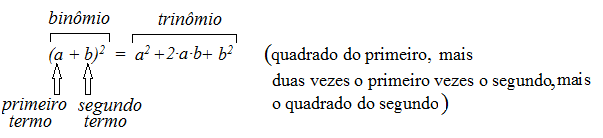
\includegraphics[width=5.91in,height=1.35in]{capitulos/equacoes_de_primeiro_e_segundo_grau/media/image2.png}
	\end{Center}
\end{figure}

Vejamos dois exemplos:

\begin{texemplo}
Determine as raízes da equação   \textit{x\textsuperscript{2} + 6x + 9 = 0}.

\textbf{Solução}: Nesse~caso, temos um TQP, pois  \textit{a = x}~ e \textit{b=3}. Portanto,

\textit{2ab = 2 $ \cdot $  x $ \cdot $ 3 = 6x}~~ que é igual ao termo intermediário do trinômio. Assim,

\textit{x\textsuperscript{2} + 6x + 9 = (x+3)\textsuperscript{2}=0}. Aplicando raiz quadrada em ambos os lados, temos:

\textit{x + 3 = 0}. Adicionando (-3) em ambos os lados, temos:

\textit{x = -3~~~ }~~é a raiz da equação dada  \qedsymbol{}
\end{texemplo}

\begin{texemplo}
Determine~as raízes da equação   \textit{x\textsuperscript{2} + 5x + 6 = 0}.

\textbf{Solução}: Nesse caso, NÃO temos um TQP, pois  se \textit{a = x}~ e  \( b=\sqrt[]{6} \) ~ não temos uma identidade, comparando com o termo intermediário do trinômio:

\textit{2ab  =  2 $ \cdot $  x $ \cdot $  \( \sqrt[]{6}~  \)  $ \neq $ ~ } \textit{5x}.

Para obter um trinômio, vamos usar \textit{a = x}~ e determinar \textit{b}, tal que

\textit{5x}~~=  \textit{2ab  =  2 $ \cdot $  x} \textit{$ \cdot $  b} ou

\textit{5}~ =\textit{  2 } \textit{$ \cdot $  b}

\textit{b}~ =\textit{ 5/2 }.

Adicionando \textit{b\textsuperscript{2} =(5/2)\textsuperscript{2}}~~ em ambos os lados da equação dada, obtemos:

 \( x^{2}+5x+ \left( \frac{5}{2} \right) ^{2}+6= \left( \frac{5}{2} \right) ^{2} \). Adicionando (\textit{-6}) em ambos os lados e reescrevendo, temos

 \( x^{2}+5x+ \left( \frac{5}{2} \right) ^{2}=\frac{1}{4} \). Fatorando o TQP obtido, temos:

 \(  \left( x+\frac{5}{2} \right) ^{2}=\frac{1}{4} \). Aplicando raiz quadrada em ambos os lados, temos:

 \( x+\frac{5}{2}= \pm \sqrt[]{\frac{1}{4}}= \pm \frac{1}{2} \). Adicionando (\textit{-5/2}) em ambos os lados e operando, temos:

 \( x= \pm \frac{1}{2}-\frac{5}{2} \) \textit{~~~ }. Finalmente, as soluções da equação dada são:

 \( x_{1}=-2  \) \textit{ ~ }~ e~~  \( x_{2}=-3  \) ~~~~~ \qedsymbol{}

\end{texemplo}

O processo desenvolvido no Ex. 5.2 pode ser generalizado da seguinte maneira:

Inicialmente, para evitar o uso de sub-índices, vamos usar \textit{A=a\textsubscript{2}~;  B=a\textsubscript{1} e C=a\textsubscript{0}}  e reescrever a  \hyperref[eqc:4.7]{Eq. (7)} :

\equacao{\textit{Ax\textsuperscript{2}~+ Bx  + C = 0}.}

Para que o coeficiente de \textit{x\textsuperscript{2}} seja \textit{1}, vamos dividir a \hyperref[eqc:4.8]{Eq. (8)} por \textit{A}.

\equacao{\( \frac{Ax^{2}+Bx+C}{A}=\frac{0}{A} \) \quad ~~~ou~   \( x^{2}+\frac{B}{A}x+\frac{C}{A}=0 \)}

Para obter o TQP, vamos usar \textit{a = x}~ e determinar \textit{b}, tal que:

 \( \frac{B}{A}x=2ab=2xb \) \textit{. }Então\textit{~~~  \( b=\frac{B}{2A} \) ~~ }.

Adicionando ( \( b^{2}= \left( \frac{B}{2A} \right) ^{2} \) ) em ambos os lados da \hyperref[eqc:4.16]{Eq. (16)}, temos

 \( x^{2}+\frac{B}{A}x+ \left( \frac{B}{2A} \right) ^{2}+\frac{C}{A}= \left( \frac{B}{2A} \right) ^{2} \). Fatorando o TQP obtido e adicionando (-C/A) em ambos os lados, temos:

 \(  \left( x+\frac{B}{2A} \right) ^{2}= \left( \frac{B}{2A} \right) ^{2}-\frac{C}{A} \). Operando o lado direito e aplicando raiz quadrada em ambos os lados, temos:

 \( x+\frac{B}{2A}=\sqrt[]{\frac{B^{2}-4AC}{4A^{2}}} \). Adicionando  \( -\frac{B}{2A}~  \) em ambos os lados, temos:

 \( x= \pm \sqrt[]{\frac{B^{2}-4AC}{4A^{2}}}-\frac{B}{2A} \) ~~~~ ou

\equacao{\( x=\frac{-B \pm \sqrt[]{B^{2}-4AC}}{2A} \) ~~ ou \quad  \( x=\frac{-a_{1} \pm \sqrt[]{a_{1}^{2}-4a_{2}a_{0}}}{2a_{2}} \)}

com os coeficientes da \hyperref[eqc:4.8]{Eq. (8)}

A \hyperref[eqc:4.17]{Eq. (17)} é conhecida como a Fórmula de Baskhara e a expressão no radicando da \hyperref[eqc:4.17]{Eq. (17)}

\textit{$ \Delta $  = B\textsuperscript{2} - 4 $ \cdot $ A $ \cdot $  C}

chama-se \textit{discriminante} e é simbolizada pela letra grega delta maiúscula (\textit{$ \Delta $ })~ \qedsymbol{}

As~equações do 2º grau tem sempre duas soluções,  \textit{x\textsubscript{1}}~e  \textit{x\textsubscript{2}}. Da fórmula de Baskhara, podemos tirar a seguinte conclusão, sobre o número de soluções das equações do 2º grau:

\begin{enumerate}
	\item Se~ \textit{$ \Delta $  = B\textsuperscript{2} -4AC = 0~~ }as soluções são reais e idênticas:~ \textit{x\textsubscript{1}}~=  \textit{x\textsubscript{2}}

	\item Se~ \textit{$ \Delta $  = B\textsuperscript{2} -4AC > 0~~ }as soluções são reais e distintas:~ \textit{x\textsubscript{1}} $ \neq $  \textit{x\textsubscript{2}}

	\item Se~ \textit{$ \Delta $  = B\textsuperscript{2}~-4AC~< 0   }as soluções não são reais.
\end{enumerate}

\subsection{Método do produto e soma}

A equação

\equacao{$x^{2} + (a+b) \cdot x + a \cdot b = 0$}

é gerada pelo produto

\equacao{$(x + a) \cdot (x + b) = 0$.}

Observemos na \hyperref[eqc:4.19]{Eq. (19)} que se os termos entre parênteses forem nulos, a equação será uma identidade. Ou seja,

\begin{enumerate}
	\item Se~~ \textit{x + a = 0}~~~~~~temos~uma solução da \hyperref[eqc:4.18]{Eq. (18)} :   \textit{x\textsubscript{1} = -a}.

	\item Se~~ \textit{x + b = 0}~~~~~~temos~outra solução da \hyperref[eqc:4.18]{Eq. (18)} :   \textit{x\textsubscript{2} = -b}.
\end{enumerate}

Assim, as soluções da \hyperref[eqc:4.18]{Eq. (18)} poder ser determinadas desde que encontremos dois números \textit{a} e \textit{b}, tal que

\textit{a + b = B\quad \quad }\textbf{(soma)}

\textit{a $ \cdot $   b = C\quad \quad }\textbf{(produto)}

\begin{texemplo}
Encontre as soluções de \textit{x\textsuperscript{2} + x - 6 = 0.}

\textbf{Solução:}~ Temos que encontrar números \textit{a} e \textit{b}, tal que

\equacao{a + b = 1}

\textit{a $ \cdot $   b = - 6. }

A solução é obtida por tentativas, por isso o método é eficiente quando as soluções são inteiras. Nesse caso, \textit{a = -2}~~e  \textit{b = 3}~satisfazem as \hyperref[eqc:4.20]{Eq. (20)}, portanto as soluções são  \textit{x\textsubscript{1} = 2} e  \textit{x\textsubscript{2} = -3}.

Observemos que as soluções têm o \textit{sinal oposto} dos números \textit{a }e\textit{ b} \qedsymbol{}
\end{texemplo}

\begin{exercicios}
\exitem{Para que ~ \textit{Ax\textsuperscript{2}~+ Bx  + C = 0}~~ seja uma equação de 2º grau, o coeficiente \textit{A}~ pode ser nulo ? e os coeficientes \textit{B} e \textit{C} ?}

\exitem{Verifique se o valor de \textit{x} dado é solução da respectiva equação:}

\begin{enumerate}[label=\alph*)]
	\item \textit{x\textsuperscript{2} 9 = 0} para \textit{x = -3} c) \textit{2x\textsuperscript{2}~~+~x - 3 = 0   }para\textit{~x~=1   }

	\item \textit{x\textsuperscript{2}~~-6x~+ 9 = 0   }para\textit{~x~= - 3   }\quad d) \textit{5x\textsuperscript{2}~ + 3x -5/2~=~0   }para\textit{ x =1/2~~ }
\end{enumerate}
\exitem{Resolva as equações usando apenas as propriedades das equações (sem usar a fórmula de Baskhara):}

\begin{enumerate}[label=\alph*)]
	\item \textit{x\textsuperscript{2} - 16 = 0\quad } \quad b) \textit{x\textsuperscript{2} +2x = 0\quad \quad }c)\textit{ -2x\textsuperscript{2} + 18 = 0}
\end{enumerate}

d) - \textit{x\textsuperscript{2} + 8x = 0\quad }\quad e) -3\textit{x\textsuperscript{2} + 6x = 0\quad }f) \textit{2x\textsuperscript{2} = 0\quad }

	\exitem{Determine \textit{B} para que as expressões sejam trinômios quadrados perfeitos:}

\begin{enumerate}[label=\alph*)]
	\item \textit{x\textsuperscript{2} +Bx +16 = 0\quad }b) \textit{x\textsuperscript{2} -Bx +9 = 0}\quad c) \textit{4t\textsuperscript{2} -Bt +9 = 0\quad \quad }
\end{enumerate}

d) 9\textit{x\textsuperscript{2} +Bx +25 = 0\quad }e) 16\textit{s\textsuperscript{2} -Bs +4 = 0}\quad f) 36\textit{x\textsuperscript{2} +Bx +9 = 0}

	\exitem{Resolva as equações usando fatoração do trinômio:}

a) \textit{x\textsuperscript{2} +4x - 5 = 0\quad }b) \textit{x\textsuperscript{2} + x - 12 = 0\quad \quad }c)~~ \textit{x\textsuperscript{2} -14x +40 = 0}

d) \textit{x\textsuperscript{2} -12x +36 = 0\quad }e) \textit{x\textsuperscript{2} -3x -  8 = 0 \quad \quad }f) 3\textit{x\textsuperscript{2} -2x - 2 = 0}

\exitem{Resolva as equações usando o método de produto e soma:}

a)~~ \textit{x\textsuperscript{2} +4x +4= 0\quad \quad }b) \textit{x\textsuperscript{2} + x - 12 = 0\quad }\quad c) \textit{x\textsuperscript{2} –3x - 10 = 0\quad }

d) \textit{x\textsuperscript{2} -7x +10 = 0 \quad }e) \textit{x\textsuperscript{2} +10x + 21 = 0~ \quad \quad }f) \textit{x\textsuperscript{2} - x - 2 = 0}

	\exitem{Verifique se o método produto e soma é eficiente para a solução de:}

\begin{enumerate}[label=\alph*)]
	\item \textit{2x\textsuperscript{2} -4x -30= 0\quad \quad \quad b) 3x\textsuperscript{2} +8x +12= 0}
\end{enumerate}

	\exitem{Resolva as equações usando a fórmula de Baskhara:}

a)~~ \textit{x\textsuperscript{2} -2x – 8 = 0\quad \quad }b)~ 4\textit{x\textsuperscript{2} +4x +1 = 0\quad } \quad c) - \textit{x\textsuperscript{2} +7x – 6 = 0}

d) 2\textit{x\textsuperscript{2} - x +3 = 0 \quad \quad }e)  \textit{x\textsuperscript{2} +5/2x +1 = 0~ \quad \quad }f) \textit{x\textsuperscript{2} - 8 = 0}

	\exitem{Determine o valor de \textit{x} para que a área da figura seja \textit{7,5 cm\textsuperscript{2}}. (medidas do desenho em centímetros)}

\begin{figure}[H]
    \centering
    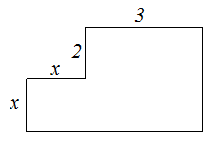
\includegraphics{capitulos/equacoes_de_primeiro_e_segundo_grau/media/image3.png}
\end{figure}

	\item{ Invente uma equação de 2º grau tal que o discriminante seja nulo.}

	\item{ Invente uma equação de 2º grau tal que:}

\begin{enumerate}[label=\alph*)]
	\item As soluções sejam reais e idênticas

	\item As soluções não sejam reais (complexas)

	\item As soluções sejam reais e distintas
\end{enumerate}

	\exitem{~ Resolva as equações usando qualquer método:}

a)~~ \textit{x(x-1)+3(x\textsuperscript{2}-1) = 0\quad \quad }\quad c)  \textit{(x+1)\textsuperscript{2} +(x – 1)\textsuperscript{ 2} = 0}

b)~~ \textit{2x(x-4)+2(x-1)= 0\quad \quad }\quad d) \textit{(x+2)\textsuperscript{ 2} + 2(x+1/2)\textsuperscript{ 2}= 0}

\end{exercicios}

\section{RESPOSTAS DOS EXERCÍCIOS PROPOSTOS}

\begin{respostas}{3}
	\ansitem{a) \textit{x = 4/3\quad \quad }}

	b) Até poderia ser usada a estratégia, porém somente após realizar a adição do lado direito.

	\ansitem{ \( x=-\frac{1}{3} \)}

	\ansitem{a)  \( -2 \) \quad \quad b) 2\quad ~~ c) 1\quad  \quad d) -2\quad \quad e) 4/6}

    f)  \( -5 \) \quad \quad g) 3\quad ~~ h) 6\quad \quad i) -10\quad \quad j) 7/2\quad

	\ansitem{\textit{x = 2}.}

	\ansitem{a)  \( x=1 \) \quad ~~ b)  \( x=\frac{5}{22} \) \quad c)  \( x=\frac{1}{7} \) \quad d)  \( x=2/5 \) \quad e) \(  x=-\frac{7}{2} \) ~~ f) \textit{x = -3.}}

    \ansitem{a)  \( 2 \) \quad \quad b)  \( -\frac{4}{3} \) \quad \quad c)  \( \frac{8}{5} \)}

    \ansitem{ \( x=1cm \)}

	\ansitem{a)  \( x=1cm \) \quad \quad \quad b)  \( x=\frac{3}{2}cm \)}


    \ansitem{ \( x=\frac{1}{2} \);}
    \ansitem{Comprimento=\textit{100m} e largura=\textit{70m};}
    \ansitem{\textit{2cm, 4cm } e \textit{ 6 cm}.}

\end{respostas}

\begin{respostas}{4}
	\ansitem{Não pois sem o coeficiente \textit{A} a equação se torna de 1º grau. Os coeficientes \textit{B} e \textit{C} podem ser nulos.}

	\ansitem{a) sim, b) não, c) o valor de \textit{x} é solução da equação, d) o valor de \textit{x} não é solução da equação}

	\ansitem{ a)  \( x= \pm 4 \) \quad \quad \quad \quad \quad d)  \( x'=0;x"=8 \)}

    \quad b)  \( x'=0;x"=-2 \) \quad \quad \quad \quad e)  \( x'=0;x"=2 \)

    \quad c)  \( x= \pm 3  \) \quad \quad \quad \quad \quad f)  \( x=0 \)

	\ansitem{a) 8\quad \quad \quad \quad \quad d) 30}

    \quad b) 6\quad \quad \quad \quad \quad e) 16

    \quad c) 12\quad \quad \quad \quad \quad f) 36\quad

	\ansitem{a)  \( x^{'}=1;x"=-5 \) \quad \quad \quad d)  \( x^{'}=6;x"=6 \)}

    \quad b)  \( x^{'}=3;x"=-4 \) \quad \quad \quad e)  \( x= \pm \sqrt[]{\frac{41}{4}}+\frac{3}{2} \)

    \quad c)  \( x^{'}=10;x"=4 \) \quad \quad \quad f)  \( x=\frac{1 \pm \sqrt[]{7}}{3} \)

	\ansitem{a)  \( x^{'}=x"=-2 \) \quad \quad \quad d)  \( x^{'}=2;x"=5 \)}

    \quad b)  \( x^{'}=3;x"=-4 \) \quad \quad \quad e)  \( x^{'}=-3;x"=-7 \)

    \quad c)  \( x^{'}=-2;x"=5 \) \quad \quad \quad f)  \( x^{'}=-1;x"=2 \)

	\ansitem{a) O método é eficiente porque as raízes são inteiras.}

    b) O método do produto e soma não é eficiente pois as raízes não são inteiras.

    \ansitem{a)  \( x^{'}=4;x"=-2 \) \quad \quad \quad d)  \( \frac{1 \pm \sqrt[]{-23})}{4} \)}

    \quad b)  \( x^{'}=-\frac{1}{2};x"=-\frac{1}{2} \) \quad \quad \quad e)  \( x^{'}=-\frac{1}{2};x^{''}=-2 \)

    \quad c)  \( x^{'}=1;~x"=6 \) \quad \quad \quad \quad f)  \( \frac{ \pm \sqrt[]{-32}}{2} \)

    \ansitem{ \( x \cong 0,4364 \)}

    \addtocounter{enumi}{2}
    \ansitem{a)  \( x^{'}=1;x"=0,75 \)}

    \quad b)  \( x^{'} \cong 3,302 \ldots ;~x" \cong -0,302 \ldots  \)

    \quad c)  \(  \pm \sqrt[]{-1} \)

    \quad d)  \( \frac{-2 \pm \sqrt[]{-2}}{2} \)

\end{respostas}

\chapter{Função do primeiro grau}

\section{Introdução}

A ideia de descrever o comportamento de uma grandeza relacionada com outra não é muito antiga. Os povos antigos, Árabes e Gregos não chegaram a investigar a velocidade. Foi com Galileo (1564-1642) ao estudar o movimento que o conceito de função começou a se configurar. Porém, não sem dificuldades. A geometria de Descartes (1637) já usava a representação gráfica de uma expressão algébrica, mas essa ideia só foi aceita na comunidade de matemáticos com os trabalhos de Euler (1707-1783) e da família dos Bernoillis, ao desenvolver o cálculo aplicado a problemas físicos. A definição atribuída a Euler diz que função \textit{é uma expressão analítica que representa a relação entre duas variáveis}. 

Um conceito de função, muito semelhante ao usado atualmente, foi introduzido por Dirichlet (1805-1859), motivado pela necessidade de uma definição mais restritiva que a de Euler, ao estudar o problema de convergência de séries, na época, aplicado à investigação de problemas de condução do calor, propostos por Fourier. A definição de Dirichlet é a seguinte: \textit{y é uma função de x, se para qualquer valor de x, existe uma regra que o associa a um único valor de y}. Em 1939, Bourbaki definiu função como \textit{regra de correspondência entre dois conjuntos e que isto era um subconjunto do produto cartesiano entre aqueles conjuntos}.

A definição de Euler é muito usada até hoje nas ciências, devido a sua simplicidade e eficiência para descrever a relação entre duas variáveis. De fato, muitas aplicações de funções na Física, Química e Economia requerem apenas uma expressão algébrica e uma representação gráfica.

Na base do desenvolvimento do Cálculo Diferencial e Integral está o conceito de função e daí sua importância, já que praticamente toda a ciência e a tecnologia moderna utilizam o Cálculo. Mas porque as funções são tão importantes para as ciências? Porque elas descrevem qualitativamente o comportamento de partes da realidade com precisão suficiente para que decisões possam ser tomadas. Saber o tempo de resfriamento de uma peça fundida é importante para decidir quando manuseá-la; saber o tempo em que a receita e a despesa de um empreendimento serão iguais, significa saber quando o lucro se inicia; o planejamento econômico de um reflorestamento depende da função de como as árvores crescem; a variação da concentração de um medicamento no organismo humano é fundamental para determinar a dose e o intervalo de ingestão; a deformação em vigas depende das cargas aplicadas e do material;... Todos esses e tantos outros fenômenos são expressos na forma de funções, cujo conhecimento básico vamos desenvolver neste capítulo.

\section{Definição de funções}

Analisemos o seguinte exemplo:

\begin{texemplo}
O preço de \textit{1 kg} de carne é \textit{R$\$$  15,00}. Determine uma fórmula para calcular qualquer o custo de quantidade de carne.

\textbf{Solução}: Vamos usar a ideia de variável. Seja \textit{x} a quantidade, em \textit{kg} e \textit{y} o custo da carne. Então

\textit{y = 15 $ \cdot $  x } \tab (2.1)
\end{texemplo}

é a expressão que dá o custo de carne para qualquer valor de \textit{x}. 

Se as massas são \textit{x = $ \{ $ 0, 0.5, 1, 2, 3$ \} $ ,} usando a Eq. (2.1) calculamos os correspondentes valores dos custos \textit{y =$ \{ $ 0, 7.5, 15, 30, 45$ \} $ }. Evidentemente, podemos calcular \textit{y} para qualquer \textit{x} real maior ou igual a zero.

\begin{texemplo}
Se \textit{x} é o lado de um quadrado, encontre uma expressão para a área.

\textbf{Solução}: Sabe-se que a área do quadrado é \textit{A = x\textsuperscript{2}}.  Para quadrados de lado \textit{x = $ \{ $ 0, 1, 2,3,4$ \} $ ,} usando a expressão da área temos os correspondentes valores de \textit{A=$ \{ $ 0,1,4,9,16$ \} $ }. Evidentemente, podemos calcular \textit{A} para qualquer  \textit{x} real maior ou igual a zero.
\end{texemplo}

\begin{caixa}
\begin{tdefinicao}
Sejam dois conjuntos \textit{X=$ \{ $ x\textsubscript{1}, x\textsubscript{2}, x\textsubscript{3}, x\textsubscript{4, }... x\textsubscript{n}$ \} $ }  e   \textit{Y=$ \{ $ y\textsubscript{1}, y\textsubscript{2}, y\textsubscript{3}, y\textsubscript{4, }..., y\textsubscript{n} $ \} $ }. Seja \textit{f  }uma regra matemática que associa os elementos de \textit{X} e \textit{Y}, formando um  conjunto de pares ordenados (\textit{x\textsubscript{i}, y\textsubscript{i}}) com \textit{i =1,2,3,4, ...,n. Y =f(x\textsubscript{i})} é uma função de \textit{X}, se para qualquer \textit{ x\textsubscript{i }, f}  associa um, e somente um valor de\textit{ y\textsubscript{i}}. 
\end{tdefinicao}
\end{caixa}

Nos pares ordenados (\textit{x,y}), os elementos do conjunto \textit{X} são chamados de \textit{abcissas} e os do conjunto \textit{Y} de \textit{ordenadas}.

\begin{figure}[H]
	\begin{Center}
		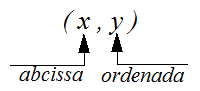
\includegraphics[width=2.08in,height=0.95in]{capitulos/funcao_do_primeiro_grau/media/image2.png}
	\end{Center}
\end{figure}

As expressões dos Exemplos 2.1 e 2.2 são funções de acordo com a Def. 2.1, pois para cada valor de \textit{x}, existe um e somente um \textit{y}. 

\begin{texemplo}
Represente a função do Exemplo 2.1 em um gráfico cartesiano.

\textbf{Solução}: Dispondo alguns valores de \textit{x} e \textit{y} em uma tabela, temos: 

\begin{figure}[H]
    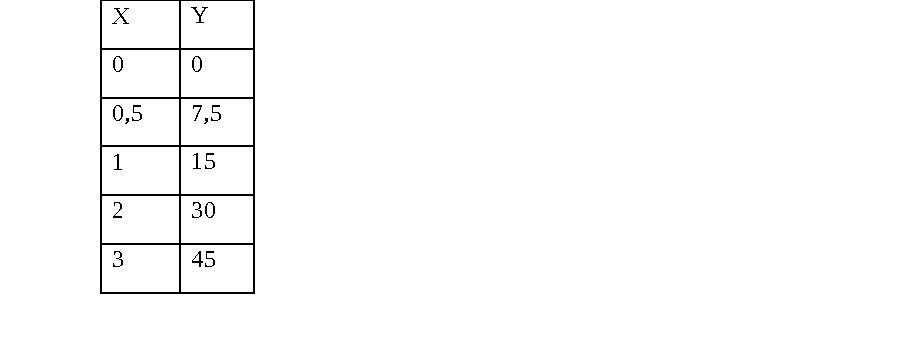
\includegraphics[width=0.45\textwidth]{capitulos/funcao_do_primeiro_grau/media/image3.pdf} 
    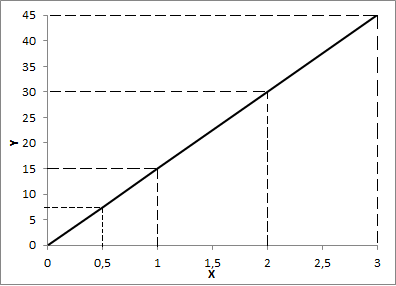
\includegraphics[width=0.45\textwidth]{capitulos/funcao_do_primeiro_grau/media/image4.png}
\end{figure}

Os valores de \textit{x} e \textit{y} formam pares ordenados (\textit{x,y}) que localizados no Plano Cartesiano, neste caso, formam uma \textbf{reta}. Como podemos usar qualquer \textit{x $ \in \mathbb{R} $, x $ \geq $  0} , a reta será contínua.

Nesse exemplo, na medida que a massa \textit{x} cresce, o custo \textit{y} também cresce, proporcionalmente. Ou seja, para cada incremento de \textit{1 kg}, o custo cresce \textit{15 reais} \qedsymbol{}
\end{texemplo}

\begin{texemplo}
Represente a função do Exemplo 2.2 em um gráfico cartesiano.

\textbf{Solução}: Dispondo alguns valores de \textit{x} e A em uma tabela, temos: 

\begin{figure}[H]
    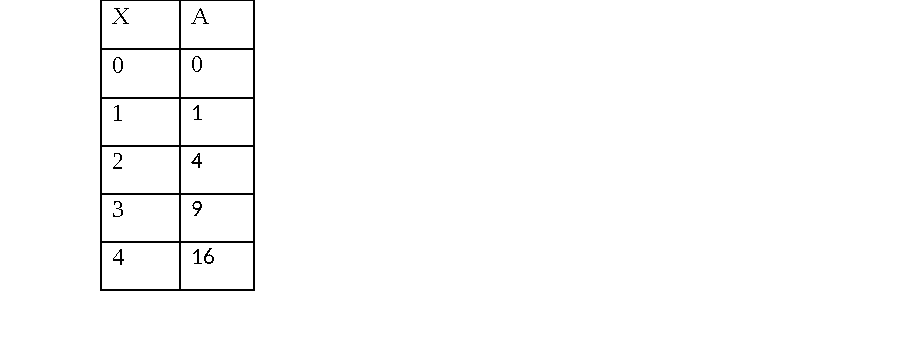
\includegraphics[width=0.45\textwidth]{capitulos/funcao_do_primeiro_grau/media/image5.pdf} 
    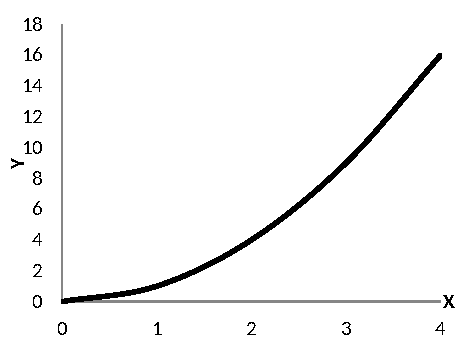
\includegraphics[width=0.45\textwidth]{capitulos/funcao_do_primeiro_grau/media/image6.pdf}
\end{figure}

Os valores de \textit{x} e \textit{A} formam pares ordenados (\textit{x,y}) que localizados no Plano Cartesiano, neste caso, formam uma \textbf{curva}. Como podemos usar qualquer \textit{x $ \in \mathbb{R} $  , x $ \geq $  0} , a curva será contínua.

Nesse exemplo, na medida que o lado \textit{x} cresce, a área \textit{A} também cresce, porém diferentemente do Exemplo 1, que tinha um crescimento constante. No primeiro incremento, a área cresceu \textit{1 cm\textsuperscript{2}}, no segundo \textit{3 cm\textsuperscript{2}}, no terceiro \textit{5 cm\textsuperscript{2}}. \qedsymbol{}
\end{texemplo}

\begin{texemplo}
Verifique se  -\textit{3x + y\textsuperscript{2} = 1} é uma função, de acordo com a Def. 2.1. Considere \textit{x $ \in \mathbb{R} $}.

\textbf{Solução}: A equação dada está na forma implícita (\textit{x} e \textit{y} estão no mesmo lado da igualdade). Para explicitar y, adicionamos (\textit{+3x}) em ambos os lados da equação, obtendo:

\textit{y\textsuperscript{2} = 1 + 3x.}

Aplicando raiz quadrada em ambos os lados da equação, temos:

 \( y= \pm \sqrt[]{1+3x} \)   .

Esta equação só terá valores reais para \textit{y}, se o radicando for um número nulo ou positivo. Então,

 \( 1+ 3x  \geq  0  \)      ou      \( x~  \geq  -1/3. \) 

\begin{figure}[H]
	\begin{Center}
		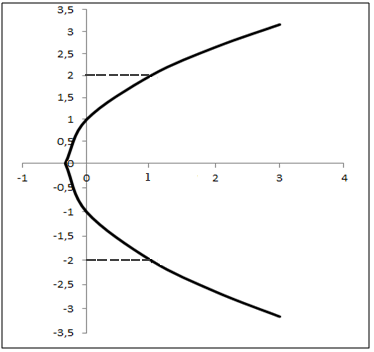
\includegraphics[width=3.9in,height=3.67in]{capitulos/funcao_do_primeiro_grau/media/image7.png}
	\end{Center}
\end{figure}

Observemos que para qualquer valor de \textit{x > -1/3}, teremos dois valores de \textit{y}. Por exemplo:

\tab Se \textit{x = 1}, teremos \textit{y = $ \pm $  2};  

\tab Se \textit{x = 2}, teremos   \( y= \pm \sqrt[]{7} \);

\tab Se \textit{x = 5}, teremos \textit{y = $ \pm $  4 }e assim por diante.   

Portanto, a equação dada não é uma função.  \qedsymbol{}
\end{texemplo}

\begin{caixa}
\textbf{Notação:}

Usa-se a notação \textit{y = f(x)} para referir-se à função \textit{f} de \textit{x}, onde \textit{x} é a variável independente e \textit{y = f(x)}  é a variável dependente de \textit{x}.

Por exemplo:   \textit{f(x) = x\textsuperscript{2}}        ou      \textit{f(x) = 3x - 2}.
\end{caixa}

\begin{caixa}
\begin{tdefinicao}
O \textit{domínio} de uma função \textit{y = f(x)} é o conjunto dos valores de \textit{x} nos quais a função é definida e denota-se:   \textit{D f(x).}
\end{tdefinicao}

\begin{tdefinicao}
A \textit{imagem} de uma função \textit{y = f(x)} é o conjunto dos valores de \textit{y }para os quais existem valores de \textit{x} correspondentes e denota-se : \textit{I\textsubscript{m} f(x).}
\end{tdefinicao}
\end{caixa}

\begin{texemplo}
Determine o domínio e a imagem da função \textit{ f(x) = x\textsuperscript{2} + 2.}

\textbf{Solução}:  Observemos que qualquer valor de \textit{x $ \in \mathbb{R} $} gera um valor de \textit{f(x)}. Então, 

\tab  \textit{Df(x)=$ \{ $ x $ \in \mathbb{R} $   } \textit{$ \} $ .}

Analisando a expressão da função, observamos que ela tem a soma de dois termos positivos (lembremos que para \textit{x\textsuperscript{2}}, teremos sempre \textit{x\textsuperscript{2}} > 0). Portanto, o menor valor possível de \textit{x\textsuperscript{2} + 2 } será \textit{2}, quando \textit{x = 0}. Então, 

\textit{I\textsubscript{m} f(x) = $ \{ $  y $ \epsilon $   \textbf{R}, y $ \geq $  2$ \} $ .}

\begin{figure}[H]
	\begin{Center}
		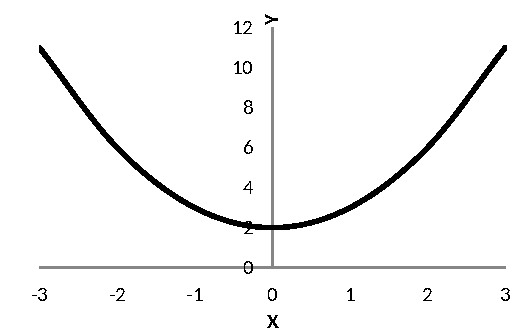
\includegraphics[width=3.5in,height=2.24in]{capitulos/funcao_do_primeiro_grau/media/image8.pdf}
	\end{Center}
\end{figure}

No gráfico de \textit{f(x)}, traçando \textit{retas verticais}, para qualquer \textit{x} teremos sempre um \textit{y} correspondente, o que indica que \textit{f(x)} é uma função.  

A imagem de \textit{f(x)} pode ser obtida traçando retas horizontais. Os valores de \textit{y}, pelos quais estas retas passarão, pertencem a imagem de \textit{f(x)}. Assim, a imagem desta função será o conjunto de números reais \textit{y }tal que  \textit{y $ \geq $  2 }\qedsymbol{}
\end{texemplo}

\begin{exercicios}
\exitem{} Localize os pontos no plano cartesiano:

\begin{multicols}{3}
a) \textit{A = (2,3)}

b) \textit{B = (-2,-3)}

c) \textit{C = (-3,3)}

d) \textit{D = (0,3)}

e)\textit{ E = (2,0)}

f) \textit{F = (0,-3)}
\end{multicols}

\exitem{} Qual é o valor de $x$ (abcissa) dos pontos sobre o eixo Y?

\exitem{} Qual é o valor de \textit{y} (ordenada) dos pontos sobre o eixo \textit{X} ?

\exitem{} Dada a função \textit{f(x) = 3x -1}, calcule:

\begin{multicols}{3}
a) \textit{f(0)}

b) \textit{f(-2)}

c) \textit{f(c+1)}

d) \textit{f(1)}

e) \textit{f(1/3)}

f) \textit{f(3-c)}
\end{multicols}

\exitem{} Dada a função \textit{f(x) = -2x +1/2}, calcule \textit{x} sendo:

\begin{multicols}{2}
a) \textit{f(x)=1/2} 

b) \textit{f(x)=1} 

c) \textit{f(x)=-3/4}

d) \textit{f(x)=4}
\end{multicols}

\exitem{} Faça o gráfico das funções com variáveis reais:

\begin{multicols}{3}
a) \textit{y = 3x}

b) \textit{f(x) = -3x +1 } 

c)  \textit{y = x\textsuperscript{2}}

d) \textit{y = x\textsuperscript{2} +1}

e)  \( g \left( x \right) =\frac{1}{x} \) 

f)  \( y=\frac{1}{x-1} \) 
\end{multicols}

\exitem{} Faça o gráfico dos dados das tabelas: 

\begin{multicols}{4}
\begin{table}[H]
a)

\begin{tabular}{p{0.2in}p{0.2in}}
\hline
%row no:1
\multicolumn{1}{|p{0.2in}}{X} & 
\multicolumn{1}{|p{0.2in}|}{Y} \\
\hhline{--}
%row no:2
\multicolumn{1}{|p{0.2in}}{-3} & 
\multicolumn{1}{|p{0.2in}|}{-6} \\
\hhline{--}
%row no:3
\multicolumn{1}{|p{0.2in}}{-2} & 
\multicolumn{1}{|p{0.2in}|}{-4} \\
\hhline{--}
%row no:4
\multicolumn{1}{|p{0.2in}}{-1} & 
\multicolumn{1}{|p{0.2in}|}{-2} \\
\hhline{--}
%row no:5
\multicolumn{1}{|p{0.2in}}{0} & 
\multicolumn{1}{|p{0.2in}|}{0} \\
\hhline{--}
%row no:6
\multicolumn{1}{|p{0.2in}}{1} & 
\multicolumn{1}{|p{0.2in}|}{2} \\
\hhline{--}
%row no:7
\multicolumn{1}{|p{0.2in}}{2} & 
\multicolumn{1}{|p{0.2in}|}{4} \\
\hhline{--}
%row no:8
\multicolumn{1}{|p{0.2in}}{3} & 
\multicolumn{1}{|p{0.2in}|}{6} \\
\hhline{--}
\end{tabular}
 \end{table}

\begin{table}[H]
b)

\begin{tabular}{p{0.2in}p{0.2in}}
\hline
%row no:1
\multicolumn{1}{|p{0.2in}}{X} & 
\multicolumn{1}{|p{0.2in}|}{Y} \\
\hhline{--}
%row no:2
\multicolumn{1}{|p{0.2in}}{-3} & 
\multicolumn{1}{|p{0.2in}|}{-5} \\
\hhline{--}
%row no:3
\multicolumn{1}{|p{0.2in}}{-2} & 
\multicolumn{1}{|p{0.2in}|}{-3} \\
\hhline{--}
%row no:4
\multicolumn{1}{|p{0.2in}}{-1} & 
\multicolumn{1}{|p{0.2in}|}{-1} \\
\hhline{--}
%row no:5
\multicolumn{1}{|p{0.2in}}{0} & 
\multicolumn{1}{|p{0.2in}|}{1} \\
\hhline{--}
%row no:6
\multicolumn{1}{|p{0.2in}}{1} & 
\multicolumn{1}{|p{0.2in}|}{3} \\
\hhline{--}
%row no:7
\multicolumn{1}{|p{0.2in}}{2} & 
\multicolumn{1}{|p{0.2in}|}{5} \\
\hhline{--}
%row no:8
\multicolumn{1}{|p{0.2in}}{3} & 
\multicolumn{1}{|p{0.2in}|}{7} \\
\hhline{--}
\end{tabular}
 \end{table}

\begin{table}[H]
c)

\begin{tabular}{p{0.2in}p{0.19in}}
\hline
%row no:1
\multicolumn{1}{|p{0.2in}}{X} & 
\multicolumn{1}{|p{0.19in}|}{Y} \\
\hhline{--}
%row no:2
\multicolumn{1}{|p{0.2in}}{-3} & 
\multicolumn{1}{|p{0.19in}|}{12} \\
\hhline{--}
%row no:3
\multicolumn{1}{|p{0.2in}}{-2} & 
\multicolumn{1}{|p{0.19in}|}{9} \\
\hhline{--}
%row no:4
\multicolumn{1}{|p{0.2in}}{-1} & 
\multicolumn{1}{|p{0.19in}|}{3} \\
\hhline{--}
%row no:5
\multicolumn{1}{|p{0.2in}}{0} & 
\multicolumn{1}{|p{0.19in}|}{1} \\
\hhline{--}
%row no:6
\multicolumn{1}{|p{0.2in}}{1} & 
\multicolumn{1}{|p{0.19in}|}{3} \\
\hhline{--}
%row no:7
\multicolumn{1}{|p{0.2in}}{2} & 
\multicolumn{1}{|p{0.19in}|}{9} \\
\hhline{--}
%row no:8
\multicolumn{1}{|p{0.2in}}{3} & 
\multicolumn{1}{|p{0.19in}|}{12} \\
\hhline{--}
\end{tabular}
 \end{table}

\begin{table}[H]
d)

\begin{tabular}{p{0.2in}p{0.19in}}
\hline
%row no:1
\multicolumn{1}{|p{0.2in}}{X} & 
\multicolumn{1}{|p{0.19in}|}{Y} \\
\hhline{--}
%row no:2
\multicolumn{1}{|p{0.2in}}{-3} & 
\multicolumn{1}{|p{0.19in}|}{5} \\
\hhline{--}
%row no:3
\multicolumn{1}{|p{0.2in}}{-2} & 
\multicolumn{1}{|p{0.19in}|}{2} \\
\hhline{--}
%row no:4
\multicolumn{1}{|p{0.2in}}{-1} & 
\multicolumn{1}{|p{0.19in}|}{1} \\
\hhline{--}
%row no:5
\multicolumn{1}{|p{0.2in}}{0} & 
\multicolumn{1}{|p{0.19in}|}{2} \\
\hhline{--}
%row no:6
\multicolumn{1}{|p{0.2in}}{1} & 
\multicolumn{1}{|p{0.19in}|}{5} \\
\hhline{--}
%row no:7
\multicolumn{1}{|p{0.2in}}{2} & 
\multicolumn{1}{|p{0.19in}|}{9} \\
\hhline{--}
%row no:8
\multicolumn{1}{|p{0.2in}}{3} & 
\multicolumn{1}{|p{0.19in}|}{14} \\
\hhline{--}
\end{tabular}
 \end{table}
\end{multicols}

\exitem{} Todas as funções do Ex.6 são funções, de acordo com a Def. 2.1?

\exitem{} A expressão  \( y = \pm \sqrt[]{x} \)    é uma função, de acordo com a Def. 2.1?

\exitem{} Faça o gráfico das funções usando uma tabela eletrônica ou um editor de gráficos computacional.

\begin{multicols}{3}
a) \textit{y = - 2x + 5}

b)  \( y=x^{2}-2x+1 \)

c) \textit{  \( y=x^{4}-x^{2}+4 \)}

d) \textit{y = x\textsuperscript{3} +1}

e) \( y=\frac{x+1}{x-1} \) \tab 

f) \( y^{2}+ x^{2}=4 \) 
\end{multicols}

\exitem{} Todas as expressões do Ex. 10 são funções, de acordo com a Def. 2.1?

\exitem{} Determine o domínio e a imagem das funções:

\begin{multicols}{3}
a) \textit{y = x}

b) \( f \left( x \right) =\frac{1}{x} \)

c) \( y=4-x^{2} \)

d)  \( f \left( x \right) =\sqrt[]{x} \)

e)  \( g \left( x \right) =-\sqrt[]{x} \)

f)  \( q \left( x \right) =\sqrt[]{x-4} \)
\end{multicols}

\item Faça os gráficos das funções do Ex. 12 usando uma ferramenta computacional.
\end{exercicios}

\section{Função do 1º grau}

Os exercícios da Seção 2 mostram que existem funções cujo gráfico é uma reta e outras apresentam curvas de diferentes formatos. Nessa seção, serão estudadas as funções cujos gráficos são retas.

Uma das características das retas é a \textit{taxa de variação (crescimento ou decrescimento) constante}. Isto significa que, para o mesmo incremento \textit{($ \Delta $ x) }em qualquer \textit{x}, o incremento \textit{($ \Delta $ y) }em \textit{y}, será o mesmo. 

\begin{texemplo}
Dada a reta \textit{f(x) = x +1 }   use o incremento \textit{$ \Delta $ x = 1 }  em

 (i) \textit{x\textsubscript{0} = 0;   }(ii)\textit{ x\textsubscript{1} = 2}  ; (iii) \textit{x\textsubscript{2} = 5 } e calcule os respectivos incrementos em \textit{y}. 

\textbf{Solução}: i) Usando o incremento em  \textit{x\textsubscript{0} = 0} :  

\textit{ x\textsubscript{0} + $ \Delta $ x = 0+1 = 1} .  

Calculando  \textit{f(x\textsubscript{0})=f(0)=0+1=1.}   Calculando a\textit{ f(x\textsubscript{0} + $ \Delta $ x)=f(1)=1+1=2.}

O incremento em \textit{y} será:\textit{  $ \Delta $ y =  f(x\textsubscript{0} + $ \Delta $ x)- f(x\textsubscript{0}) =  2 - 1 = 1.}

ii) Usando o incremento em  \textit{x\textsubscript{1} = 2} :  

\textit{x\textsubscript{1} + $ \Delta $ x = 2 +1  = 3} .  

Calculando  \textit{f(x\textsubscript{1})=f(2)=2+1=3.}   Calculando a\textit{ f(x\textsubscript{1} + $ \Delta $ x)=f(3)=3+1=4.}

O incremento em \textit{y} será:\textit{  $ \Delta $ y =  f(x\textsubscript{1} + $ \Delta $ x)- f(x\textsubscript{1}) =  4 - 3 = 1.  }

iii) Usando o incremento em  \textit{x\textsubscript{2} = 5 } 

\textit{x\textsubscript{2} + $ \Delta $ x = 5+1  = 6} .  

Calculando  \textit{f(x\textsubscript{2})=f(5)=5+1=6.}   Calculando a\textit{ f(x\textsubscript{2} + $ \Delta $ x)=f(6)=6+1=7.}

O incremento em \textit{y} será:\textit{  $ \Delta $ y =  f(x\textsubscript{2} + $ \Delta $ x)- f(x\textsubscript{2}) =  7 - 6 = 1.  }

Como podemos observar, o incremento \textit{$ \Delta $ y}  foi o mesmo, nos três casos analisados: \textit{$ \Delta $ y=1}

Faça um gráfico mostrando os incrementos \textit{$ \Delta $ x} e  nos valores de \textit{x} dados.\qedsymbol{}
\end{texemplo}

\begin{caixa}
\begin{tdefinicao}
Uma função polinomial do primeiro grau tem a forma

\textit{y = f(x) = ax + b} \tab (3.1)

onde \textit{a} e \textit{b} são números reais, \textit{x} e \textit{y} são variáveis reais.

O coeficiente \textit{a}  é chamado \textbf{coeficiente angular (inclinação)} e o \textit{b} \textbf{coeficiente linear}.
\end{tdefinicao}
\end{caixa}

\begin{texemplo}
Faça os gráficos das funções: (i)  \textit{ f(x) = x + 1  ;  }(ii) \textit{ g(x) = 2x + 1; }(iii) \textit{h(x) = 3x + 1.}

\textbf{Solução:} Elaborando tabelas para as três funções e localizando os pares ordenados no Plano Cartesiano, obtemos três retas.  

\begin{figure}[H]
	\begin{Center}
		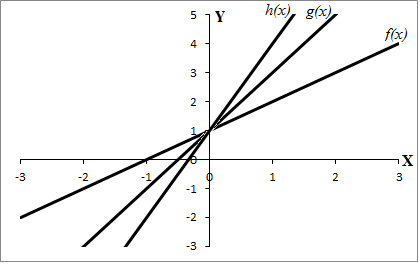
\includegraphics[width=4.38in,height=2.77in]{capitulos/funcao_do_primeiro_grau/media/image9.png}
	\end{Center}
\end{figure}

Observemos que as inclinações são diferentes, sendo que a diferença entre as três funções é o \textit{coeficiente angular}. Observemos que quanto maior o \textit{a} mais inclinada está a reta \qedsymbol{}
\end{texemplo}

\begin{caixa}
O coeficiente angular é a \textit{inclinação (ou taxa de crescimento)} da reta, dado pela expressão:

\begin{FlushRight}
 \( a=tg \left(  \theta  \right) =\frac{ \Delta y}{ \Delta x}=\frac{y_{i}-y_{i+1}}{x_{i}-x_{i+1}} \) \tab (3.2)
\end{FlushRight}

Onde \textit{i = 0,1,2,3,...} refere-se aos pontos de \textit{f(x)} e  é o ângulo que a reta faz com o eixo \textit{X}.
\end{caixa}

\begin{figure}[H]
	\begin{Center}
		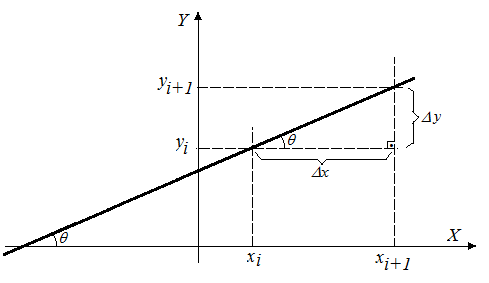
\includegraphics[width=5.09in,height=2.95in]{capitulos/funcao_do_primeiro_grau/media/image10.png}
	\end{Center}
\end{figure}

\begin{texemplo}
Faça os gráficos das funções: (i)  \textit{ f(x) = x + 1  ;  }(ii) \textit{ g(x) = x + 2; }(iii) \textit{h(x) = x + 3.}

\textbf{Solução:} Elaborando tabelas para as três funções e localizando os pares ordenados no Plano Cartesiano, obtemos três retas.

\begin{figure}[H]
	\begin{Center}
		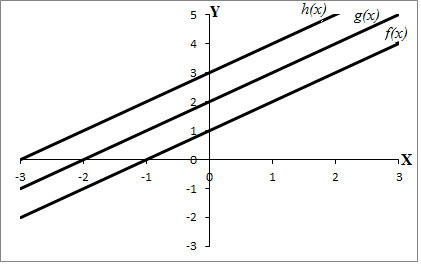
\includegraphics[width=4.39in,height=2.75in]{capitulos/funcao_do_primeiro_grau/media/image11.png}
	\end{Center}
\end{figure}

Observemos que todas têm a mesma inclinação, pois os coeficientes angulares são iguais: \textit{a = 1}.

Observemos também que quando calculamos as funções para \textit{x = 0} (pontos sobre o eixo \textit{Y}) o valor obtido é o coeficiente linear: \textit{f(0) = 1; g(0) = 2  }e\textit{  h(0) = 3}.  Podemos concluir que o \textit{coeficiente linear} é o valor do \textit{y}, nos pontos onde a reta corta o eixo \textit{Y}  \qedsymbol{}
\end{texemplo}

\begin{caixa}
O \textit{coeficiente linear} é o valor do \textit{y }(ordenada), no ponto (\textit{0,b}) onde a reta corta o eixo \textit{Y}  
\end{caixa}

\begin{texemplo}
Uma reta passa pelos pontos: \textit{P\textsubscript{1} = (1,2) }e\textit{ P\textsubscript{2} = (3,5):}

i) Calcule o coeficiente angular

ii) Calcule o coeficiente linear.

\textbf{Solução: }(i) Usando a Eq. (3.2) temos:

 \[ a=\frac{5-2}{3-1}=\frac{3}{2} \] 

(ii) Substituindo o valor de \textit{a} na Eq. (3.2), temos:

 \( y=\frac{3}{2}x+b \) \tab (3.3)

Como a reta passa pelos pontos \textit{P\textsubscript{1 }}e\textit{ P\textsubscript{2}}, as coordenadas desses pontos devem satisfazer a Eq. (3.3). Usando as coordenadas de\textit{ P\textsubscript{1} = (1,2) }na Eq. (3.3), temos:

\textit{\( 2=\frac{3}{2} \cdot 1+b \)}. Resolvendo para\textit{ b, }temos\textit{:}

\( b=\frac{1}{2} \)  

Observemos que se fosse utilizado o ponto \textit{P\textsubscript{2} = (3,5)} , obteríamos o mesmo valor de \textit{b}  \qedsymbol{}
\end{texemplo}

\subsection{Crescimento e decrescimento das funções do 1º grau}

O quadro abaixo define o que são funções crescentes e decrescentes:

\begin{caixa}
Seja \textit{y = f(x)} uma função definida no intervalo \textit{(x\textsubscript{0},x\textsubscript{n}).} 

Se \textit{f(x\textsubscript{i+1}) > f(x\textsubscript{i})} para qualquer \textit{x\textsubscript{i }} $ \in $  \textit{(x\textsubscript{0},x\textsubscript{n}} ) então \textit{f} é \textit{crescente} em \textit{(x\textsubscript{0},x\textsubscript{n}).}

Se \textit{f(x\textsubscript{i+1}) <  f(x\textsubscript{i})} para qualquer \textit{x\textsubscript{i }} $ \in $  \textit{(x\textsubscript{0},x\textsubscript{n})} então \textit{f}é  de\textit{crescente} em \textit{(a,b).}
\end{caixa}

 O quadro abaixo apresenta a relação entre coeficiente angular e crescimento da função do 1º grau:

\begin{caixa}
Se o \textit{coeficiente angular} é \textit{positivo} a reta é crescente.

Se o \textit{coeficiente angular} é \textit{negativo }a reta é decrescente.
\end{caixa}

\begin{texemplo}
Verifique se as retas são crescentes ou decrescentes. 

i) \textit{f(x) = 3x - 5}

ii) \textit{f(x) = - x + 2}

iii) \textit{4 = 3x -2y}

\textbf{Solução:}

(i) O coeficiente angular da reta é \textit{+3}. Portanto a reta é crescente para qualquer \textit{x $ \in \mathbb{R}$.}

(ii)  O coeficiente angular da reta é \textit{-1}. Portanto a reta é decrescente para qualquer \textit{x $ \in \mathbb{R} $.}

(iii) A equação está na forma implícita. Adicionando (\textit{+2y}) e (\textit{-4}) em ambos os lados, obtemos:

\textit{\tab 2y = 3x - 4. }Dividindo a equação por \textit{2}, obtemos:   \( y=\frac{3}{2}x-2 \) . 

O coeficiente angular da reta é \textit{+3/2}. Portanto a reta é crescente para qualquer \textit{x $\in \mathbb{R}.$}\qedsymbol{}
\end{texemplo}

\subsection{Domínio e imagem da função de 1º grau}

\begin{caixa}
As funções de 1º grau têm a expressão de um polinômio, cujas operações são possíveis para qualquer \textit{x} real. Assim, o domínio destas funções é:

\textit{Df(x)= $ \{ $ x $ \in \mathbb{R} $ $ \} $ } .

Como as funções de 1º grau são estritamente crescentes ou decrescentes e não tem descontinuidades, sua imagem é

\textit{Imf(x)= $ \{ $ y $ \in \mathbb{R} $  $ \} $ .}
\end{caixa}

\subsection{Raiz da função de 1º grau}

\begin{caixa}
\begin{tdefinicao}
	A raiz de uma função é o valor do \textit{x}, do ponto onde a função intercepta o eixo \textit{X}.
\end{tdefinicao}
\end{caixa}

A raiz das funções de 1º grau é determinada fazendo \textit{y=f(x)=0} na Eq. (3.1), de acordo com a Def. 3.2, pois os pontos sobre o eixo \textit{X}, tem \textit{y = 0}. Assim, 

\textit{0 = ax + b} . Resolvendo para \textit{x}, temos:

\begin{caixa}
 \( x=-\frac{b}{a} \) \tab (raiz da função de 1º grau)
\end{caixa}

\begin{texemplo}
Determine a raiz da função  \textit{5 = -2x - y}  e mostre-a no gráfico da função.

\textbf{Solução:} Mesmo com a equação na forma implícita, colocamos a exigência da Def. 3.1 \textit{y = 0}  na função dada e obtemos: 

\textit{\tab 5 = -2x - 0} .  Resolvendo para \textit{x}, temos   \textit{x = -5/2}, que é a raiz da função. 

\begin{figure}[H]
	\begin{Center}
		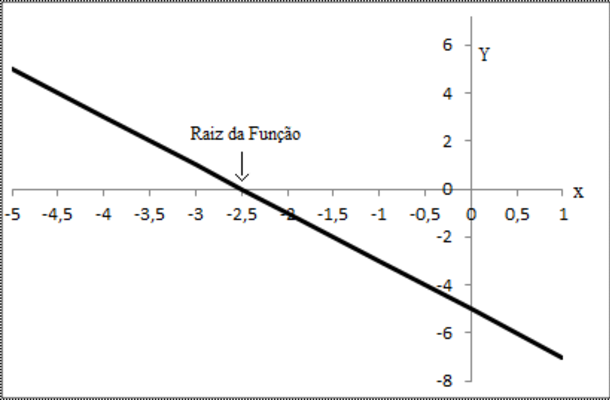
\includegraphics[width=4.41in,height=2.79in]{capitulos/funcao_do_primeiro_grau/media/image12.pdf}
	\end{Center}
\end{figure}

A Fig. 3.5 mostra a raiz da função no ponto (\textit{-5/2,0}) de interceptação do eixo \textit{X}  \qedsymbol{}
\end{texemplo}

\subsection{Sinal da função de 1º grau}

Lembremos que os valores de \textit{y} são os valores da função. Portanto, o sinal da função em algum ponto é o sinal das ordenadas, nos pontos da função.

\begin{texemplo}
Dada a função \textit{y = f(x) = x - 3}, determine o sinal da função para os seguintes valores de \textit{x: -1, 0, 1,2,3,4,5}.

\textbf{Solução}: Substituindo os valores de \textit{x} dados em \textit{f(x)}, obtemos os respectivos valores de \textit{y}, apresentados na tabela.

\begin{table}[H]
 			\centering
\begin{tabular}{p{0.69in}p{0.27in}p{0.27in}p{0.27in}p{0.27in}p{0.67in}p{0.29in}p{0.19in}}
\hline
%row no:1
\multicolumn{1}{|p{0.69in}}{X} & 
\multicolumn{1}{|p{0.27in}}{-1} & 
\multicolumn{1}{|p{0.27in}}{0} & 
\multicolumn{1}{|p{0.27in}}{1} & 
\multicolumn{1}{|p{0.27in}}{2} & 
\multicolumn{1}{|p{0.67in}}{3} & 
\multicolumn{1}{|p{0.29in}}{4} & 
\multicolumn{1}{|p{0.19in}|}{5} \\
\hhline{--------}
%row no:2
\multicolumn{1}{|p{0.69in}}{Y} & 
\multicolumn{1}{|p{0.27in}}{-4} & 
\multicolumn{1}{|p{0.27in}}{-3} & 
\multicolumn{1}{|p{0.27in}}{-2} & 
\multicolumn{1}{|p{0.27in}}{-1} & 
\multicolumn{1}{|p{0.67in}}{0} & 
\multicolumn{1}{|p{0.29in}}{+1} & 
\multicolumn{1}{|p{0.19in}|}{+2} \\
\hhline{--------}
%row no:3
\multicolumn{1}{|p{0.69in}}{Sinal de Y} & 
\multicolumn{1}{|p{0.27in}}{\textit{-}} & 
\multicolumn{1}{|p{0.27in}}{\textit{-}} & 
\multicolumn{1}{|p{0.27in}}{\textit{-}} & 
\multicolumn{1}{|p{0.27in}}{\textit{-}} & 
\multicolumn{1}{|p{0.67in}}{Sem sinal} & 
\multicolumn{1}{|p{0.29in}}{+} & 
\multicolumn{1}{|p{0.19in}|}{+} \\
\hhline{--------}

\end{tabular}
 \end{table}

Observemos que o sinal dos valores da função (\textit{y}) são negativos para \textit{x < 3} e positivos para \textit{x > 3}. A mudança do sinal ocorreu em \textit{x = 3}, que é a raiz da função.

\begin{figure}[H]
	\begin{Center}
		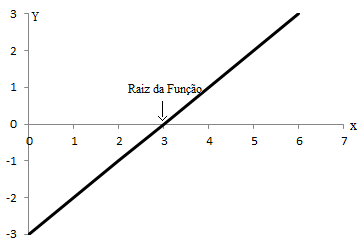
\includegraphics[width=3.75in,height=2.56in]{capitulos/funcao_do_primeiro_grau/media/image13.png}
	\end{Center}
\end{figure}

A visualização do sinal é evidente no gráfico, assim como a mudança do sinal a partir da raiz da função  \qedsymbol{}
\end{texemplo}

\begin{texemplo}
Determine o sinal das funções: (i)  \textit{ f(x) = x - 1} e  (ii)  \textit{ g(x) = -x - 1}.

\textbf{Solução}: No Exemplo 3.7 observamos que o sinal da função muda quando a função intercepta o eixo X (raiz da função). Então, vamos calcular as raízes das funções e ver a inclinação das mesmas.

\textbf{(i)} Raiz de \textit{f(x)}:    \( x=-\frac{b}{a}=-\frac{-1}{1}=1 \) . 

Como \textit{f(x)} é inclinada para a direita (crescente, pois \textit{a = 1 > 0}) , \textit{f(x) } é negativa se \textit{x < 1} e positiva se \textit{x > 1}.

\begin{figure}[H]
	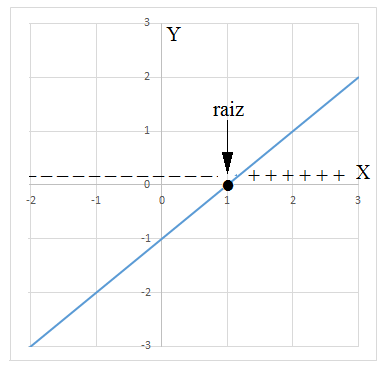
\includegraphics[width=0.45\textwidth]{capitulos/funcao_do_primeiro_grau/media/image14.png} 
	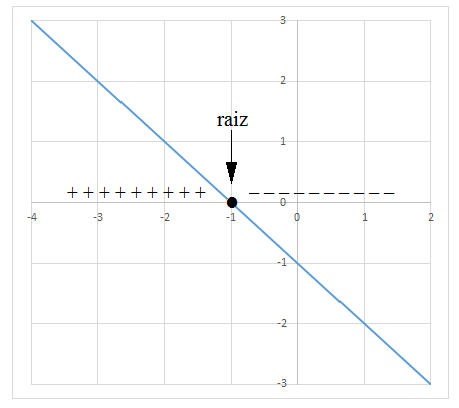
\includegraphics[width=0.45\textwidth]{capitulos/funcao_do_primeiro_grau/media/image15.png}
\end{figure}

\textbf{(ii)} Raiz de $g(x): x = -\frac{a}{b} = -\frac{-1}{-1} = -1$.

Como \textit{f(x)} é inclinada para a esquerda (decrescente, pois \textit{a = -1 < 0}) , \textit{f(x) } é positiva se \textit{x < -1} e negativa  se \textit{x > -1}  \qedsymbol{}
\end{texemplo}

\begin{caixa}
\textbf{SINAL DA FUNÇÃO DO 1º GRAU}

Seja \textit{y = f(x)=ax + b, }cuja raiz é\textit{  \( x_{r}=-\frac{b}{a} \)  .}

Se \textit{a > 0}  então:  \textit{f(x) }é \textbf{negativa } para\textit{ x < x\textsubscript{r}  }e  \textit{f(x) }é \textbf{positiva} para\textit{ x > x\textsubscript{r}.}

Se \textit{a < 0}  então:  \textit{f(x) }é \textbf{positiva } para\textit{ x < x\textsubscript{r}  }e  \textit{f(x) }é \textbf{negativa} para\textit{ x > x\textsubscript{r}.}
\end{caixa}

\subsection{Tipos especiais de retas}

\subsubsection{Função constante}

As \textit{retas horizontais} são chamadas funções constantes, pois não crescem nem decrescem. Seu coeficiente angular, pela Eq. (3.2) será nulo, portanto sua equação será:

\begin{caixa}
\textit{y = b, para b $ \in \mathbb{R} $}. \tab (3.4)
\end{caixa}

Observemos que para \textit{b = 0}, temos \textit{y = 0}, que é o próprio eixo \textit{X}.

Se \textit{f(x)=c}  o \textit{Df(x)=}$ \{ $ \textit{ x $\in \mathbb{R}$} $ \} $  e a imagem é    \textit{I\textsubscript{m}f(x) =} $ \{ $ \textit{ y $\in \mathbb{R}$} / \textit{y = b }$ \} $ .

\begin{texemplo}
Faça o gráfico das funções: 

i) \textit{y = 3} \tab (ii) \textit{y = -2}

\textbf{Solução:}

\begin{figure}[H]
	(i) 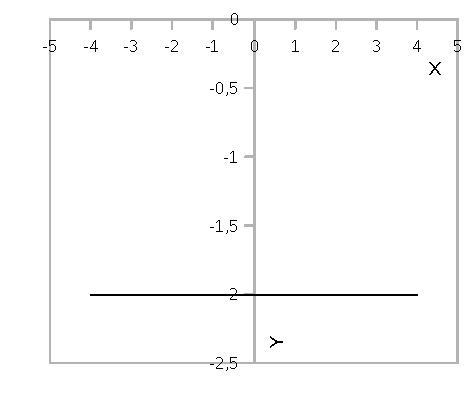
\includegraphics[width=0.45\textwidth]{capitulos/funcao_do_primeiro_grau/media/image16.pdf} 
	(ii) 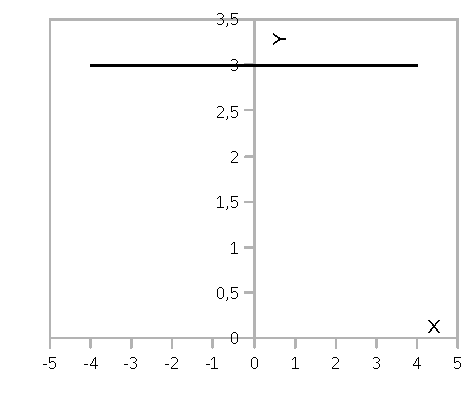
\includegraphics[width=0.45\textwidth]{capitulos/funcao_do_primeiro_grau/media/image17.pdf}
\end{figure}
\end{texemplo}

Todas as funções dadas são funções constantes (retas paralelas a \textit{X}, ou retas horizontais). Mesmo variando os valores de \textit{x}, os valores de \textit{y} permanecem constantes. \qedsymbol{} 

\subsubsection{Retas verticais}

Estas retas, de acordo com a definição de função (Def. 2.1) NÃO SÃO FUNÇÕES, pois para o mesmo \textit{x}, correspondem vários valores de \textit{y}. Tão pouco, são funções do 1º grau. Observemos que, não existe coeficiente angular, porque a Eq. (3.2) teria denominador nulo. Assim, a expressão para as retas verticais não deriva da forma da Eq.(3.1). 

A expressão para as retas verticais é construída com base no fato da abcissa ser constante para qualquer valor da ordenada, \textit{y}. Então:

\begin{caixa}
\textit{x = c}, onde  \textit{c} é uma constante. \tab (3.5)
\end{caixa}

\begin{texemplo}
Faça o gráfico das retas: 

i) \textit{x = 3} \qquad (ii) \textit{x = -1}

\textbf{Solução:}

\begin{figure}[H]
	i) 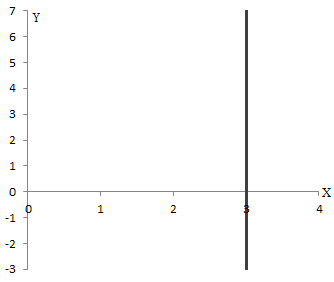
\includegraphics[width=0.45\textwidth]{capitulos/funcao_do_primeiro_grau/media/image18.png} 
	ii) 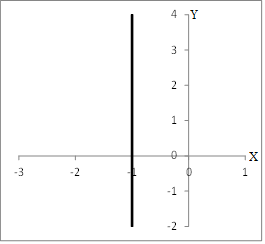
\includegraphics[width=0.45\textwidth]{capitulos/funcao_do_primeiro_grau/media/image19.png}
\end{figure}
\end{texemplo}

\subsubsection{Função identidade}

Esta função tem esse nome porque os valores de \textit{x} e \textit{y} são iguais. Sua expressão é:

\begin{caixa}
\textit{y = x}. \tab (3.6)
\end{caixa}

Se \textit{f(x) = x}  o domínio \textit{Df(x)=}$ \{ $ \textit{ x $ \in \mathbb{R} $} $ \} $  e a imagem é \textit{I\textsubscript{m}f(x) =} $ \{ $ \textit{ y $ \in \mathbb{R} $} $ \} $ \qedsymbol{}

\begin{texemplo}
Faça o gráfico da função  \textit{y = x}.

\textbf{Solução:} A função identidade divide na metade o 1º e o 3º quadrantes do Plano Cartesiano. O ângulo que esta reta faz com o eixo \textit{X} é \textit{45º }\qedsymbol{}

\begin{figure}[H]
	\begin{Center}
		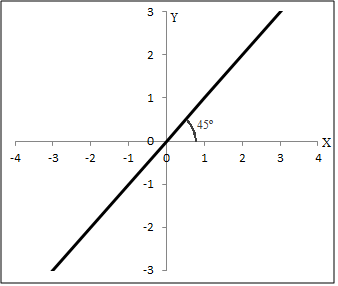
\includegraphics[width=3.52in,height=2.98in]{capitulos/funcao_do_primeiro_grau/media/image20.png}
	\end{Center}
\end{figure}
\end{texemplo}

\subsubsection{Função linear}

As funções do 1º grau, com \textit{a $ \neq $   0}  e \textit{b = 0} são chamadas funções lineares e têm a forma:

\begin{FlushRight}
\textit{y = ax.} \tab (3.7)
\end{FlushRight}

Se \textit{f(x) = ax}  o \textit{Df(x)=}$ \{ $ \textit{ x $ \in \mathbb{R} $} $ \} $  e a imagem é    \textit{I\textsubscript{m}f(x) =} $ \{ $ \textit{ y $\in \mathbb{R}$} $ \} $ .

\subsubsection{Função afim}

As funções do 1º grau, com \textit{a $ \neq $   0}  são chamadas \textbf{função afim} e têm a forma:

\begin{FlushRight}
\textit{y = ax + b.} \tab (3.8)
\end{FlushRight}

Se \textit{f(x) = ax} \textit{+ b} o \textit{Df(x)=}$ \{ $ \textit{ x $\in \mathbb{R}$} $ \} $  e a imagem é \textit{I\textsubscript{m}f(x) =} $ \{ $ \textit{ y $\in \mathbb{R}$} $ \} $ .

Observemos que as funções lineares são também funções afim.

\begin{texemplo}
Faça o gráfico da função  \textit{y = 4x}.

\textbf{Solução:} Como as funções lineares têm  \textit{b = 0}, então interceptam os eixos na origem (\textit{0,0}). O coeficiente angular igual a \textit{+4} indica que a função é crescente (inclinada para a direita), com inclinação \textit{+4}, portanto passará pelo ponto (\textit{1,4}). Colocando estes dados no Plano Cartesiano, obtemos o gráfico indicado na Fig. 3.14.

\begin{figure}[H]
	\begin{Center}
		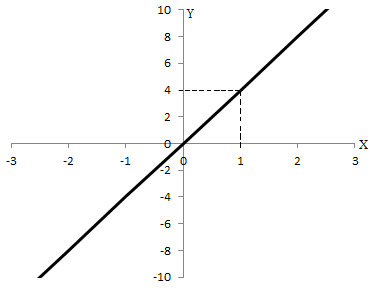
\includegraphics[width=3.12in,height=2.44in]{capitulos/funcao_do_primeiro_grau/media/image21.png} \qedsymbol{}
	\end{Center}
\end{figure}
\end{texemplo}

\subsection{Retas paralelas e perpendiculares}

\begin{caixa}
Sejam as retas    (\textit{r) :}   \textit{y = mx + b}   e   (\textit{s) :}   \textit{y = px + c}    . 

Se \textit{r} é \textbf{paralela} a \textit{s} então  \textit{m = p}. 

Se \textit{r} é \textbf{perpendicular} a  \textit{s}  então \( p=-\frac{1}{m} \)   .
\end{caixa}

\begin{exercicios}
\exitem{} Verifique se a dependência entre as grandezas mencionadas é de 1º grau:

\begin{enumerate}[label=\alph*)]
	\item Considere que a distribuição de adubo em uma lavoura é homogênea. A quantidade de adubo distribuída é proporcional a área de lavoura?

	\item A circunferência de um círculo é proporcional ao seu raio? E a área?

	\item O lixo produzido por uma cidade é proporcional ao número de habitantes?

	\item Uma caixa d’água é enchida por uma torneira, sempre com a mesma abertura. O volume de água da caixa é proporcional ao tempo? 

	\item No planejamento de uma festa, a quantidade de comida é proporcional à quantidade de pessoas?
\end{enumerate}

\exitem{} A tabela abaixo apresenta a deformação \textit{y } (\textit{cm}) de uma mola que está sendo distendida por massas \textit{m}, (\textit{g}) penduradas. Verifique se \textit{m} é proporcional a \textit{y}. 

\begin{table}[H]
 			\centering
\begin{tabular}{p{0.49in}p{0.29in}p{0.29in}p{0.29in}p{0.29in}p{0.29in}}
\hline
%row no:1
\multicolumn{1}{|p{0.49in}}{\textit{y}, (\textit{cm})} & 
\multicolumn{1}{|p{0.29in}}{0} & 
\multicolumn{1}{|p{0.29in}}{3} & 
\multicolumn{1}{|p{0.29in}}{6} & 
\multicolumn{1}{|p{0.29in}}{9} & 
\multicolumn{1}{|p{0.29in}|}{12} \\
\hhline{------}
%row no:2
\multicolumn{1}{|p{0.49in}}{\textit{m} (\textit{g})} & 
\multicolumn{1}{|p{0.29in}}{0} & 
\multicolumn{1}{|p{0.29in}}{50} & 
\multicolumn{1}{|p{0.29in}}{100} & 
\multicolumn{1}{|p{0.29in}}{150} & 
\multicolumn{1}{|p{0.29in}|}{200} \\
\hhline{------}

\end{tabular}
 \end{table}

\exitem{} Considerando que o custo de uma corrida de taxi \textit{(y)} depende de um valor fixo \textit{(b)}, referente à hora do dia, do preço por quilômetro percorrido (\textit{p}) e da quilometragem percorrida (\textit{x}). Fazendo \textit{b = 5,00} reais e \textit{p = 1,5} reais, determine uma função para o custo \textit{y(x)} de uma corrida.

\exitem{} Determine uma função que relacione o custo dos azulejos para revestir uma parede com \textit{x} \textit{m\textsuperscript{2}}, sendo que o preço de \textit{1} \textit{m\textsuperscript{2}}   de azulejo é \textit{p}.

\exitem{} O custo (\textit{C}) da carne usada para um churrasco depende do preço da carne (\textit{p}), da quantidade de carne comprada (\textit{x}) e da gasolina gasta para ir ao supermercado (\textit{b}). Faça uma função \textit{C(x)}.

\exitem{} O custo (\textit{C}) para produzir uma certa mercadoria é a soma dos custos fixos (\textit{CF}) e dos variáveis (\textit{a}) , aqueles que dependem da quantidade produzida (\textit{x}). Faça uma função \textit{C(x)}.

\exitem{} Determine os coeficientes angular e linear das retas que passam pelos pontos dados e construa a função do 1º grau:

\begin{multicols}{2}
	a) \textit{P\textsubscript{1} = (-1,0)}  e  \textit{P\textsubscript{2} = (3,2)}

	b) \textit{P\textsubscript{1} = (0,3)}  e  \textit{P\textsubscript{2} = (-3,0)}

	c) \textit{P\textsubscript{1} = (2,-2)}  e  \textit{P\textsubscript{2} = (-2,2)}

	d) \textit{P\textsubscript{1} = (3,3)}  e  \textit{P\textsubscript{2} = (5,3)}
\end{multicols}

\exitem{} Para produzir 5 peças de uma certa mercadoria foram gastos R$\$$  15,00. Para produzir 12 peças foram gastos R$\$$  35,00.  Supondo que os custos são proporcionais ao número de peças:

a) Determine uma função de 1º grau que relacione custos e número de peças

b) Determine o custo para 30 peças. 

\exitem{} Determine o coeficiente angular das funções e verifique se são crescentes ou decrescentes:

\begin{multicols}{2}
a) \textit{3x + y = 3}

b)  \( \frac{1}{2}x+y=4 \)

c)  \( \frac{3}{2}y+x=\frac{2}{3} \)

d)  \( \frac{x-y}{2}=3 \)
\end{multicols}

\exitem{} Dados os pontos da tabela, verifique se eles estão alinhados. Se estiverem, determine a equação da função linear e faça o gráfico.

\begin{multicols}{2}
\begin{table}[H]
\begin{tabular}{p{0.2in}p{0.18in}p{0.19in}p{0.16in}p{0.1in}}
\hline
%row no:1
\multicolumn{1}{|p{0.2in}}{X} & 
\multicolumn{1}{|p{0.18in}}{0} & 
\multicolumn{1}{|p{0.19in}}{1} & 
\multicolumn{1}{|p{0.16in}}{3} & 
\multicolumn{1}{|p{0.1in}|}{6} \\
\hhline{-----}
%row no:2
\multicolumn{1}{|p{0.2in}}{Y} & 
\multicolumn{1}{|p{0.18in}}{1} & 
\multicolumn{1}{|p{0.19in}}{3/2} & 
\multicolumn{1}{|p{0.16in}}{5/2} & 
\multicolumn{1}{|p{0.1in}|}{4} \\
\hhline{-----}
\end{tabular}
 \end{table}

\begin{table}[H]
\begin{tabular}{p{0.2in}p{0.18in}p{0.19in}p{0.16in}p{0.16in}}
\hline
%row no:1
\multicolumn{1}{|p{0.2in}}{X} & 
\multicolumn{1}{|p{0.18in}}{0} & 
\multicolumn{1}{|p{0.19in}}{1} & 
\multicolumn{1}{|p{0.16in}}{2} & 
\multicolumn{1}{|p{0.16in}|}{3} \\
\hhline{-----}
%row no:2
\multicolumn{1}{|p{0.2in}}{Y} & 
\multicolumn{1}{|p{0.18in}}{1,5} & 
\multicolumn{1}{|p{0.19in}}{2,5} & 
\multicolumn{1}{|p{0.16in}}{3,5} & 
\multicolumn{1}{|p{0.16in}|}{4,6} \\
\hhline{-----}
\end{tabular}
 \end{table}
\end{multicols}

\exitem{} Considere um quadrado cujos vértices estão nos pontos \textit{V\textsubscript{1} = (0,0)} ;   \textit{V\textsubscript{2} = (0,4);  V\textsubscript{3} = (4,4)}  e  \textit{V\textsubscript{4} = (4,0). }Determine equações para as retas correspondentes a cada lado do quadrado.

\exitem{} Considere um triângulo cujos vértices estão nos pontos \textit{V\textsubscript{1}=(1,1)} ; \textit{V\textsubscript{2}=(4,1) }e\textit{ V\textsubscript{3}=(1,4). }Determine equações para as retas correspondentes a cada lado do triângulo.

\exitem{} Dadas as equações de retas, faça o gráfico usando somente as informações fornecidas pelos coeficientes angular e linear (não use tabela):

\begin{multicols}{2}
a) \textit{y = -x + 1}

b) \textit{y = 4x}

c) \textit{y = -x}

d)  \textit{y = 2x - 3}

e) \textit{y = 1}

f) \textit{x = 1}
\end{multicols}

\exitem{} Construa a equação e faça um esboço do gráfico das retas \textit{y = ax + b}, com as informações dadas:

\begin{multicols}{2}
a) \textit{a = 2} e \textit{b = 1}

b) \textit{a = -1}  e passa em \textit{(1,0)}

c) passa em \textit{(0,0)} e tem inclinação \textit{-2}

d) é constante e passa em \textit{(2,3)}

e)  $\theta = 45\degree$ e \textit{b = -1}

f)  $\theta = 120\degree$ e passa em \textit{(0,3)}
\end{multicols}

\exitem{} a) Um motoqueiro cobra R$\$$  3,00 por viagem, para entregar até cinco pizzas. Sabendo que o custo de uma pizza é R$\$$  40,00, faça uma função que dê o custo de 1 a 5 pizzas. Faça o gráfico da função.

b) Refaça a função para o custo de uma pizza é R$\$$  50,00. Faça o gráfico e compare com a reta da letra (a).

\exitem{} Analise os coeficientes angular e linear das retas. Determine se as retas crescem ou decrescem e o ponto de intersecção com o eixo Y. Faça um esboço do gráfico com base nessa análise.

\begin{multicols}{3}
a) \textit{y = 3x + 5}

b) \textit{y = -2,3x - 1}

c)\textit{y = 2x - 1, 3}

d) \textit{y = -5,2x + 2,3}

e) \textit{y = -1, 3x + 2}

f) \textit{y = -4, 1x-5}
\end{multicols}

\exitem{} Nas retas que passam pelos pontos $P_1$ e $P_2$, determine se a reta cresce ou decresce e o ponto em que a reta intercepta o eixo Y:

\begin{multicols}{2}
a) \textit{P\textsubscript{1 }=(1,1) }e \textit{P\textsubscript{2 }=(2,4)}

b)\textit{ P\textsubscript{1}=(1,6) }e \textit{P\textsubscript{2 }=(5,3)}

c)\textit{ P\textsubscript{1}=(2,8) }e \textit{P\textsubscript{2 }=(7,1)}

d)\textit{ P\textsubscript{1}=(6,1) }e \textit{P\textsubscript{2 }=(1,3)}
\end{multicols}

\exitem{}  A fabricação de um produto implica em custos de materiais, energia, mão de obra, encargos sociais e impostos comerciais. Para uma determinada quantidade do produto, vamos considerar os custos de mão de obra como custo fixo, no valor de R$\$$  20,00. Considerando que os custos de materiais, energia e impostos são de R$\$$  150,00, para produzir uma unidade do produto:

a) Construa uma tabela relacionando o número de unidades do produto e o custo total.

b) Faça um gráfico com os dados da tabela.

c) Determine uma equação para relacionar o número de unidades do produto e o custo total.

d) Determine o coeficiente angular e o linear. Qual é o significado destes coeficientes no problema?

\exitem{} Uma agência de pesquisa estatística encontrou os percentuais de voto (V) mostrados na tabela abaixo para os candidatos A e B.

\begin{table}[H]
 			\centering
\begin{tabular}{p{0.26in}p{0.73in}p{0.83in}p{0.83in}}
%row no:1
\multicolumn{1}{p{0.26in}}{Data} & 
\multicolumn{1}{p{0.73in}}{Tempo(dias)} & 
\multicolumn{2}{p{0.83in}}{V ($\%$ )} \\
\hhline{~~~~}
%row no:2
\multicolumn{1}{p{0.26in}}{} & 
\multicolumn{1}{p{0.73in}}{} & 
\multicolumn{1}{p{0.83in}}{Candidato (A)} & 
\multicolumn{1}{p{0.83in}}{Candidato (B)} \\
\hhline{~~~~}
%row no:3
\multicolumn{1}{p{0.26in}}{01/07} & 
\multicolumn{1}{p{0.73in}}{1} & 
\multicolumn{1}{p{0.83in}}{35} & 
\multicolumn{1}{p{0.83in}}{30} \\
\hhline{~~~~}
%row no:4
\multicolumn{1}{p{0.26in}}{01/08} & 
\multicolumn{1}{p{0.73in}}{32} & 
\multicolumn{1}{p{0.83in}}{37} & 
\multicolumn{1}{p{0.83in}}{32} \\
\hhline{~~~~}
%row no:5
\multicolumn{1}{p{0.26in}}{01/09} & 
\multicolumn{1}{p{0.73in}}{63} & 
\multicolumn{1}{p{0.83in}}{46} & 
\multicolumn{1}{p{0.83in}}{40} \\
\hhline{~~~~}

\end{tabular}
 \end{table}

a) Faça um gráfico do percentual de voto (V) pelo tempo (t) para os dois candidatos, considerando o período 1/07 a 1/09.

b) Considere o percentual de voto uma função linear em cada mês e determine a função da reta do mês de julho. Com esta função, calcule o percentual para o dia 20 de julho.

c) Se a variável V mantiver em setembro a mesma tendência de agosto, para os dois candidatos, quais serão os percentuais de voto no dia 16 de setembro?
\end{exercicios}

\section{Aplicações de funções do 1º grau }

\subsection{Produção de bens: custo fixo + custo variável}

A produção de bens, seja na indústria ou na agricultura, apresenta custos variáveis e fixos. Os primeiros dependem da quantidade de bens produzidos e os últimos não dependem. Por exemplo, na produção de vinho, o custo das garrafas, matéria prima (uva), impostos, energia, água e produtos de limpeza são \textbf{variáveis}, ou seja, dependem da quantidade produzida. Quanto mais litros de vinhos forem produzidos, estes custos aumentarão proporcionalmente. Enquanto que o custo do aluguel, mão-de-obra, o equipamento (pipas, bomba, baldes, máquina de colocar rolhas,...) são \textbf{constantes} até uma certa quantidade de litros produzidos. 

Um modelo linear pode ser usado para modelar a produção de bens:

\begin{FlushRight}
\textit{\tab C(x) = p} \textit{x + CF} \tab (4.1)
\end{FlushRight}

Onde \textit{C(x) }é o custo total\textit{ (R$\$$ ), x }é a quantidade produzida (\textit{unidades})\textit{, p }é o custo variável por unidade produzida\textit{ (R$\$$ /unidade) }e\textit{ CF }é o custo fixo\textit{ (R$\$$ ).}

Observemos que a Eq. 4.1 é uma função afim, onde \textit{p} e \textit{CF} são os coeficientes angular e linear, respectivamente.

A Receita (ou ganhos com a venda do bem produzido) é proporcional à quantidade produzida e vendida. Assim, a função receita é uma função linear:

\begin{FlushRight}
\textit{R(x) = PV } \textit{x} \tab (4.2)
\end{FlushRight}

Onde \textit{R(x)} é a receita (\textit{R$\$$ }) e \textit{PV} é o preço de venda de cada bem (\textit{R$\$$ /unidade}).

Para determinar o Lucro da atividade, fazemos a diferença entre a receita e o custo de produção. 

\begin{Center}
\textit{L(x)= R(x) - C(x) = PVx -(p }\textit{x + CF)} ou
\end{Center}

\textit{L(x)=  (PV  - p)x - CF}. \tab (4.3)

Observemos que a Eq. 4.3 também é uma função afim.

Considere que para produzir um litro de vinho o custo variável por unidade é \textit{p = R$\$$  4,50}, o custo fixo é \textit{CF = R$\$$  2.000,00} e o preço de venda é \textit{PV = R$\$$  10,00}.

\begin{enumerate}
	\item Substitua os valores de \textit{p}, \textit{CF} e \textit{PV} nas Eqs. 4.1, 4.2 e 4.3  e faça os gráficos das funções \textit{C}, \textit{R} e \textit{L}, no mesmo plano cartesiano.

	\item Calcule quantos litros de vinho deverão ser produzidos para que a receita seja equivalente aos custos \qedsymbol{}
\end{enumerate}

\subsection{Produção de Lixo}

A Tabela abaixo apresenta dados sobre a produção de lixo doméstico em Chapecó em 2004, 2007 e 2012.

\begin{table}[H]
 			\centering
\begin{tabular}{p{1.67in}p{0.88in}p{1.28in}p{1.28in}}
\hline
%row no:1
\multicolumn{1}{|p{1.67in}}{Tempo, \textit{t} (anos)} & 
\multicolumn{1}{|p{0.88in}}{2004} & 
\multicolumn{1}{|p{1.28in}}{2007} & 
\multicolumn{1}{|p{1.28in}|}{2012} \\
\hhline{----}
%row no:2
\multicolumn{1}{|p{1.67in}}{População, \textit{h} (habitantes)} & 
\multicolumn{1}{|p{0.88in}}{165.220} & 
\multicolumn{1}{|p{1.28in}}{168.113} & 
\multicolumn{1}{|p{1.28in}|}{180.000} \\
\hhline{----}
%row no:3
\multicolumn{1}{|p{1.67in}}{Resíduos domésticos, \textit{R}    { (kg/hab./dia)}} & 
\multicolumn{1}{|p{0.88in}}{0,405} & 
\multicolumn{1}{|p{1.28in}}{0,630} & 
\multicolumn{1}{|p{1.28in}|}{0,855} \\
\hhline{----}

\end{tabular}
 \end{table}

Fonte: Abrelpe; MMA\tab (Dados citados pelas alunas Ana C. Maccari e Cristiane L. da Silva  no trabalho de Cálculo Numérico, Curso de Engenharia Ambiental, 2º/2014)

\begin{enumerate}
	\item Verifique se a população cresce linearmente com o tempo.

	\item Verifique se a produção de resíduos domésticos/habitante/dia cresce linearmente com o tempo.

	\item Considerando que \textit{R(h)} é linear entre 2007 e 2016, faça a previsão da \textit{R(2016)} \qedsymbol{}
\end{enumerate}

\subsection{Modelo Mola-massa}

Um sistema mola-massa é ilustrado na figura abaixo uma mola é distendida por massas \textit{m}, (\textit{g}) que causam deformações  \textit{y } (\textit{cm}). A posição \textit{y\textsubscript{o}} \textit{= 0} corresponde ao estado da mola sem massa. A cada massa \textit{m\textsubscript{i}} colocada corresponde uma posição \textit{y\textsubscript{i}} (deformação da mola), sendo \textit{i = 0,1,2,3,.. n} , o número de massas. Para o regime elástico (valores de \textit{m}, para os quais a mola ainda volta na posição \textit{y\textsubscript{o}}) as posições \textit{y} são proporcionais às massas \textit{m}. Considerando o conceito de força peso, que é a força com que a terra atrai as massas, temos

\textbf{F}\textit{ = m$ \cdot $  }\textbf{g}

Onde \textit{m} é a massa (\textit{g})  \textbf{g} a aceleração da gravidade (\textit{m/s\textsuperscript{2}}).

A relação entre \textit{F} e \textit{y}  é uma função de 1º grau, conhecida como Lei de Hooke

\textit{\tab F(y) = k y} ,   

onde \textit{k} é uma constante característica da mola. Observemos que \textit{k} é o coeficiente angular da função e neste caso, tem um significado físico: a $``$dureza$"$  da mola.

\begin{figure}[H]
	\begin{Center}
		\includegraphics[width=2.06in,height=2.38in]{capitulos/funcao_do_primeiro_grau/media/image22.png}
	\end{Center}
\end{figure}

\begin{enumerate}
	\item Considere molas com \textit{k = 1,2 e 3}. Calcule as deformações \textit{y} para as massas 

\textit{m = 0,50,100,150 }e\textit{ 200 g}. (considere \textbf{g}\textit{ = 10} \textit{m/s\textsuperscript{2}})

	\item Faça um gráfico e compare as retas.

	\item Qual é a mola mais $``$dura$"$  \qedsymbol{}
\end{enumerate}

\subsection{Locação de carros}

A consulta a um site de locação de carros resultou nos dados da tabela abaixo. 

\begin{table}[H]
 			\centering
\begin{tabular}{p{0.88in}p{1.28in}}
\hline
%row no:1
\multicolumn{1}{|p{0.88in}}{Nº de diárias} & 
\multicolumn{1}{|p{1.28in}|}{Valor cobrado (R$\$$ )} \\
\hhline{--}
%row no:2
\multicolumn{1}{|p{0.88in}}{\Centering 1} & 
\multicolumn{1}{|p{1.28in}|}{\Centering 83} \\
\hhline{--}
%row no:3
\multicolumn{1}{|p{0.88in}}{\Centering 2} & 
\multicolumn{1}{|p{1.28in}|}{\Centering 166} \\
\hhline{--}
%row no:4
\multicolumn{1}{|p{0.88in}}{\Centering 3} & 
\multicolumn{1}{|p{1.28in}|}{\Centering 249} \\
\hhline{--}
%row no:5
\multicolumn{1}{|p{0.88in}}{\Centering 4} & 
\multicolumn{1}{|p{1.28in}|}{\Centering 332} \\
\hhline{--}
%row no:6
\multicolumn{1}{|p{0.88in}}{\Centering 5} & 
\multicolumn{1}{|p{1.28in}|}{\Centering 415} \\
\hhline{--}

\end{tabular}
 \end{table}

\begin{enumerate}
	\item Verifique se o valor cobrado (\textit{V}) é proporcional ao número de diárias (\textit{d}). Faça um modelo matemático que relacione \textit{V} e \textit{d}. Calcule \textit{V} para um aluguel de sete dias.

	\item Como ficaria este modelo se a locadora cobrasse uma taxa de lavagem de R$\$$  25,00.

	\item Outro sistema de aluguel considera uma taxa fixa de R$\$$  40,00, mais R$\$$  1,30 por quilômetro rodado. Faça um modelo matemático para este sistema de locação.

	\item Considerando a locação por quilômetro rodado (letra (d)), se um locador pretende ficar 3 dias com o carro, quanto quilômetros ele teria que rodar para que o custo seja equivalente ao do modelo da letra (c) ?

	\item Verifique qual é o sistema de locação mais vantajoso para uma semana de locação, com 400 km rodados.
\end{enumerate}

\subsection{Orçamento de Churrasco}

Consideremos as seguintes hipóteses de consumo para um churrasco:

- 450 g de carne por pessoa, 

- preço médio da carne: PM,

- custo da salada: 20$\%$  do custo da carne.

O custo médio de carne e salada por pessoa (\textit{p}) pode ser calculado fazendo:

\textit{p} = custo da carne + custo salada      

\textit{p = 0,450 $ \cdot $  PM  + 0,450 $ \cdot $  PM $ \cdot $  0,2 = 1,2 $ \cdot $  0,450 $ \cdot $  PM}   ou

\textit{p =  0,54 PM}

O custo de um churrasco (\textit{C}) para um grupo de pessoas depende do número de pessoas (\textit{x}), do custo da carne e salada por pessoa (\textit{p}) e da taxa de limpeza (\textit{b}) do local do churrasco.

\begin{FlushRight}
\textit{C(x) = p} \textit{x + b}. \tab (4.4)
\end{FlushRight}

\begin{enumerate}
	\item Qual é o custo de um churrasco para \textit{10} pessoas, considerando o preço médio da carne \textit{PM = R$\$$  18,00}.

	\item Que modificação na Eq. 4.4 deve ser implementada para incluir o custo da  gasolina (\textit{g}) usada para buscar os mantimentos?

	\item Que modificação na Eq. 4.4 deve ser implementada para incluir o custo da  sobremesa (\textit{SM})?
\end{enumerate}

\subsection{Deslocamento com velocidade constante}

As funções de 1º grau são úteis para modelar vários problemas de Física, como por exemplo o deslocamento de um carro em uma estrada retilínea, com velocidade constante. A velocidade (\textit{v}) é definida como a razão entre a variação da distância percorrida (\textit{x}) pela variação de tempo (\textit{t}):

\begin{FlushRight}
 \( v=\frac{ \Delta x}{ \Delta t} \) \tab (4.5)
\end{FlushRight}

Se  \textit{x\textsubscript{f}  }e\textit{ x\textsubscript{i}} são as posições final e inicial do carro (ver Fig. 4.6.1), substituindo \textit{$ \Delta $ x=x\textsubscript{f} - x\textsubscript{i}} , na Eq. (4.5), temos

\begin{FlushRight}
\textit{x\textsubscript{f} = v$ \cdot $ $ \Delta $ x + x\textsubscript{i}} \tab (4.6)
\end{FlushRight}

\begin{figure}[H]
	\begin{Center}
		\includegraphics[width=4.8in,height=1.33in]{capitulos/funcao_do_primeiro_grau/media/image23.png}
	\end{Center}
\end{figure}

Se o tempo inicial for zero  \textit{$ \Delta $ x = t , }onde t é o tempo de deslocamento e \textit{x\textsubscript{f}}   é a posição final, ou seja, uma função de \textit{x(t)}. Então,

\begin{FlushRight}
\textit{X(t) = v$ \cdot $ t + x\textsubscript{i}} \tab (4.7)
\end{FlushRight}

\begin{enumerate}
	\item Determine a posição de um carro que partiu do quilômetro \textit{10} com velocidade constante \textit{80 km/h} e andou durante \textit{3 h}.

	\item Quanto tempo esse carro precisará rodar nessa velocidade para chegar no quilômetro 270 ?
\end{enumerate}

\subsection{Temperatura no interior de uma parede}

Consideremos que a parede de uma casa está sujeita a temperaturas diferentes e constantes, na superfície interna e externa da casa, durante um período de tempo. Se as temperaturas forem mantidas, a distribuição de temperatura no interior da parede será linear. 

\begin{figure}[H]
	\begin{Center}
		\includegraphics[width=2.64in,height=2.98in]{capitulos/funcao_do_primeiro_grau/media/image24.png}
	\end{Center}
\end{figure}

Seja \textit{d} a espessura da parede. Com base no sistema de coordenadas mostrado na figura acima, dois pontos da reta \textit{T(x)} são conhecidos. Então, podemos calcular o coeficiente angular: 

\begin{FlushRight}
 \( a=\frac{T_{e}-T_{i}}{ \Delta x}=\frac{ \Delta T}{d} \) \tab (4.8)
\end{FlushRight}

Como a reta intercepta o eixo das ordenadas em \textit{T = T\textsubscript{i}}  temos:

\begin{FlushRight}
 \( T \left( x \right) =\frac{ \Delta T}{d}x+T_{i} \) \tab (4.9)
\end{FlushRight}

\begin{enumerate}
	\item Determine uma função  \textit{T(x) }em uma parede, sabendo que \textit{45ºC } e \textit{25ºC} são as temperaturas externa interna da casa, respectivamente e a espessura da parede é de \textit{15 cm}.

	\item Usando a função do item (a), calcule a temperatura em \textit{5} \textit{cm}, \textit{7,5} \textit{cm} e \textit{10 cm}.
\end{enumerate}

\section{RESPOSTAS DOS EXERCÍCIOS PROPOSTOS}

\begin{respostas}{2}
\begin{figure}[H]
\ansitem{}

\includegraphics[width=3.2in,height=2.52in]{capitulos/funcao_do_primeiro_grau/media/image25.jpeg}
\end{figure}
\ansitem{}  \( x=0 \) 

\ansitem{}  \( y=0 \) 

\ansitem{}

\begin{multicols}{3}
a)  \( f \left( 0 \right) =-1 \)

b)  \( f \left( -2 \right) =-7 \)

c)  \( f \left( c+1 \right) =3c+2 \)

d)  \( f \left( 1 \right) =2 \)

e)  \( f \left( 1/3 \right) =0 \) 

f)  \( f \left( 3-c \right) =-3c+8 \) 
\end{multicols}

\ansitem{}

\begin{multicols}{2}
a)  \( x= 0  \)

b) \( x=-1/4 \)

c)  \( x=5/8 \)

d)  \( x=-7/4 \)
\end{multicols}

\begin{figure}[H]
	\ansitem{}

	a) \includegraphics[width=0.45\textwidth]{capitulos/funcao_do_primeiro_grau/media/image26.png} 
	b) \includegraphics[width=0.45\textwidth]{capitulos/funcao_do_primeiro_grau/media/image27.png}
\end{figure}

\begin{figure}[H]
	c) \includegraphics[width=0.45\textwidth]{capitulos/funcao_do_primeiro_grau/media/image28.pdf} 
	d) \includegraphics[width=0.45\textwidth]{capitulos/funcao_do_primeiro_grau/media/image29.pdf}
\end{figure}

\begin{figure}[H]
	e) \includegraphics[width=0.45\textwidth]{capitulos/funcao_do_primeiro_grau/media/image30.png} 
	f) \includegraphics[width=0.45\textwidth]{capitulos/funcao_do_primeiro_grau/media/image31.png}
\end{figure}

\begin{figure}[H]
	\ansitem{}

	a) \includegraphics[width=0.45\textwidth]{capitulos/funcao_do_primeiro_grau/media/image32.png} 
	b) \includegraphics[width=0.45\textwidth]{capitulos/funcao_do_primeiro_grau/media/image33.png}
\end{figure}

\begin{figure}[H]
	c)\includegraphics[width=0.45\textwidth]{capitulos/funcao_do_primeiro_grau/media/image34.pdf} 
	d) \includegraphics[width=0.45\textwidth]{capitulos/funcao_do_primeiro_grau/media/image35.pdf}
\end{figure}

\ansitem{} Sim.

\ansitem{} Não, pois para um mesmo valor de \textit{x} há dois valores de \textit{y} correspondentes.

\begin{figure}[H]
	\ansitem{}

	a) \includegraphics[width=0.45\textwidth]{capitulos/funcao_do_primeiro_grau/media/image36.pdf} 
	b) \includegraphics[width=0.45\textwidth]{capitulos/funcao_do_primeiro_grau/media/image37.pdf}
\end{figure}

\begin{figure}[H]
	c) \includegraphics[width=0.45\textwidth]{capitulos/funcao_do_primeiro_grau/media/image38.png} 
	d) \includegraphics[width=0.45\textwidth]{capitulos/funcao_do_primeiro_grau/media/image39.png}
\end{figure}

\begin{figure}[H]
	e) \includegraphics[width=0.45\textwidth]{capitulos/funcao_do_primeiro_grau/media/image40.png} 
	f) \includegraphics[width=0.45\textwidth]{capitulos/funcao_do_primeiro_grau/media/image41.png}
\end{figure}

\ansitem{} Não, a alternativa f) não está de acordo, pois há dois valores de \textit{y} para mesmo \textit{x.}

\ansitem{} a)  \( D= \left\{ x \in R \right\} ; ~~~ Im= \{ y \in R \}  \)

b)  \( D= \left\{ x \in R \neq 0 \right\} ;~~~~~~ Im= \{ y \in  R / y \neq 1 \}  \) 

c)  \( D= \left\{ x \in R \right\} ; Im= \{ y \in R / y \leq 4 \}  \) 

d)  \( D= \left\{ x \in R/x \geq 0 \right\} ; Im= \{ y \in R/y \geq 0 \}  \) 

e)  \( D= \left\{ x \in R/x \geq 0 \right\} ; Im= \{ y \in R/y \leq 0 \}  \) 

f)  \( D= \left\{ x \in R/x \geq 4 \right\} ; Im= \{ y \in R/y \geq 0 \}  \) 
\end{respostas}

\begin{respostas}{3}
\ansitem{} a) Sim. A dependência é de 1º Grau.

b) A proporção da circunferência em relação ao raio é de 1º Grau. A da área é de 2º Grau.

c) Sim. A dependência é de 1º Grau.

d) Sim. A dependência é de 1º Grau.

e) Sim. A dependência é de 1º Grau.

\ansitem{} \textit{m }é proporcional a \textit{y.  \(  \Delta y/ \Delta x=50/3 \) }

\ansitem{}  \( y \left( x \right) =1,5x+5 \) 

\ansitem{}  \( C \left( x \right) =p \cdot x \) ; 

\ansitem{}  \( C \left( x \right) =px+b \) 

\ansitem{}  \( C \left( x \right) =ax+CF \) 

\ansitem{} a)  \( a=1/2; b= 1/2 \) ;  \( f \left( x \right) =\frac{1}{2}x+\frac{1}{2} \) \tab \tab 

b)  \( a=1; b= 3; \)   \( f \left( x \right) =x+3 \) \tab \tab 

c) \(  a= -1; b= 0; \)   \( f \left( x \right) =-x \) \tab \tab 

d) \(  a= 0; b= 3; f \left( x \right) =3 \) 

\ansitem{} a) C=20/7x +5/7 \qquad b) C(30)=605/7= 86,43

\ansitem{}

\begin{multicols}{2}
a)  \( a=-3; Decrescente \)

b)  \( a=-1/2; Decrescente \) 

c)  \( a= -2/3; Decrescente \)

d) \(  a=1; Crescente \)
\end{multicols}

\ansitem{} a) \( f \left( x \right) =\frac{1}{2}x+1 \)  

\begin{figure}[H]
	\begin{Center}
		\includegraphics[width=3.07in,height=1.91in]{capitulos/funcao_do_primeiro_grau/media/image42.pdf}
	\end{Center}
\end{figure}

b) Os pontos não estão alinhados

\ansitem{}  \textit{V\textsubscript{1}V\textsubscript{2}:x=0; V\textsubscript{1}V\textsubscript{4}:y=0; V\textsubscript{2}V\textsubscript{3}:y=4; V\textsubscript{3}V\textsubscript{4}:x=4}

\ansitem{}  \textit{V\textsubscript{1}V\textsubscript{2}:y=1; V\textsubscript{1}V\textsubscript{3}:x=1; V\textsubscript{2}V\textsubscript{3}:y=-x+5}

\begin{figure}[H]
	\ansitem{}

	a) \includegraphics[width=0.45\textwidth]{capitulos/funcao_do_primeiro_grau/media/image43.png} 
	b) \includegraphics[width=0.45\textwidth]{capitulos/funcao_do_primeiro_grau/media/image44.png}
\end{figure}

\begin{figure}[H]
	c) \includegraphics[width=0.45\textwidth]{capitulos/funcao_do_primeiro_grau/media/image45.png} 
	d) \includegraphics[width=0.45\textwidth]{capitulos/funcao_do_primeiro_grau/media/image46.png}
\end{figure}

\begin{figure}[H]
	e) \includegraphics[width=0.45\textwidth]{capitulos/funcao_do_primeiro_grau/media/image47.png} 
	f) \includegraphics[width=0.45\textwidth]{capitulos/funcao_do_primeiro_grau/media/image48.png}
\end{figure}

\begin{figure}[H]
	\ansitem{}

	a) \includegraphics[width=0.45\textwidth]{capitulos/funcao_do_primeiro_grau/media/image49.png} 
	b) \includegraphics[width=0.45\textwidth]{capitulos/funcao_do_primeiro_grau/media/image50.png}
\end{figure}

\begin{figure}[H]
	c) \includegraphics[width=0.45\textwidth]{capitulos/funcao_do_primeiro_grau/media/image51.png} 
	d) \includegraphics[width=0.45\textwidth]{capitulos/funcao_do_primeiro_grau/media/image52.png}
\end{figure}

\begin{figure}[H]
	e) \includegraphics[width=0.45\textwidth]{capitulos/funcao_do_primeiro_grau/media/image53.png} 
	f) \includegraphics[width=0.45\textwidth]{capitulos/funcao_do_primeiro_grau/media/image54.png}
\end{figure}

\ansitem{} a)  \( f \left( x \right) =40x+3 \)  \qquad b)  \( g \left( x \right) =50x+3 \) 

\begin{figure}[H]
	\includegraphics[width=0.45\textwidth]{capitulos/funcao_do_primeiro_grau/media/image55.png} 
	\includegraphics[width=0.45\textwidth]{capitulos/funcao_do_primeiro_grau/media/image56.png}
\end{figure}

\ansitem{} a) Crescente; Intersecção em Y: (0,5) \qquad b) Decrescente; Intersecção em Y: (0,-1)

\begin{figure}[H]
	\includegraphics[width=0.45\textwidth]{capitulos/funcao_do_primeiro_grau/media/image57.pdf} 
	\includegraphics[width=0.45\textwidth]{capitulos/funcao_do_primeiro_grau/media/image58.pdf}
\end{figure}

c) Crescente; Intersecção em Y: (0,-1.3) \qquad d) Decrescente; Intersecção em Y:(0,2.3)

\begin{figure}[H]
	\includegraphics[width=0.45\textwidth]{capitulos/funcao_do_primeiro_grau/media/image59.pdf} 
	\includegraphics[width=0.45\textwidth]{capitulos/funcao_do_primeiro_grau/media/image60.pdf}
\end{figure}

e) Decrescente; Intersecção em Y:(0,2) \qquad f) Decrescente; Intersecção em Y:(0,-5)

\begin{figure}[H]
	\includegraphics[width=0.45\textwidth]{capitulos/funcao_do_primeiro_grau/media/image61.pdf} 
	\includegraphics[width=0.45\textwidth]{capitulos/funcao_do_primeiro_grau/media/image62.pdf}
\end{figure}

\ansitem{} a) Crescente; Ponto de Intersecção em Y= -2

 b) Decrescente; Ponto de Intersecção em Y=27/4

 c) Decrescente; Ponto de Intersecção em Y=54/5

 d) Decrescente; Ponto de Intersecção em Y=17/5

\ansitem{}

\begin{multicols}{2}
\begin{table}[H]
a)

\begin{tabular}{p{0.37in}p{0.39in}}
\hline
%row no:1
\multicolumn{1}{|p{0.37in}}{X} & 
\multicolumn{1}{|p{0.39in}|}{Y} \\
\hhline{--}
%row no:2
\multicolumn{1}{|p{0.37in}}{0} & 
\multicolumn{1}{|p{0.39in}|}{20} \\
\hhline{--}
%row no:3
\multicolumn{1}{|p{0.37in}}{1} & 
\multicolumn{1}{|p{0.39in}|}{170} \\
\hhline{--}
%row no:4
\multicolumn{1}{|p{0.37in}}{5} & 
\multicolumn{1}{|p{0.39in}|}{770} \\
\hhline{--}
%row no:5
\multicolumn{1}{|p{0.37in}}{10} & 
\multicolumn{1}{|p{0.39in}|}{1520} \\
\hhline{--}
%row no:6
\multicolumn{1}{|p{0.37in}}{50} & 
\multicolumn{1}{|p{0.39in}|}{7520} \\
\hhline{--}
\end{tabular}
 \end{table}

\begin{figure}[H]
	b)
	
	\includegraphics[width=2.88in,height=2.24in]{capitulos/funcao_do_primeiro_grau/media/image63.png}
\end{figure}
\end{multicols}

 c)  \( C(x)=150x+20 \) \tab d)150 é o custo de produção de uma peça e 20 \tab é o custo unitário. 

\ansitem{}

\begin{figure}[H]
	a)
	
	\includegraphics[width=2.79in,height=1.8in]{capitulos/funcao_do_primeiro_grau/media/image64.png}
\end{figure}

b) Candidato (A):  \( y=\frac{2}{31}x+\frac{1083}{31} \) , Percentual para 20/07: 36,22$\%$ 

Candidato (B):  \( y=\frac{2}{31}x+\frac{928}{31} \) , Percentual para 20/07: 31,22$\%$ 

c) Candidato (A): 51,8$\%$ 

Candidato (B): 45,1$\%$ 
\end{respostas}

\section{ANEXO}

\subsection{Tangente de ângulos suplementares}

Sejam o ângulo \textit{0 <  < 90º}. O suplementar de   é (\textit{180º - }). Pela definição de tangente,  \( tg \left(  \theta  \right) =MT \)   e  \( tg \left( 180 ^{\circ} - \theta  \right) =MT' \)  , como mostra a Fig. 1. Os ângulos dos triângulos OMT e OMT’ são iguais e o segmento OM é comum aos triângulos (portanto são iguais) então os outros lados também serão. Portanto, os triângulos OMT e OMT’ são idênticos e 

 \[ tg \left(  \theta  \right) =-tg \left( 180 ^{\circ} - \theta  \right)  \] 

\begin{figure}[H]
	\begin{Center}
		\includegraphics[width=3.08in,height=2.64in]{capitulos/funcao_do_primeiro_grau/media/image65.png}
	\end{Center}
\end{figure}

Figura 1 - Tangente de ângulos suplementares

\subsection{Tangente de ângulos complementares}

Pela definição de tangente, temos:

 \( tg \left(  \theta  \right) =\frac{QR}{PR} \)        e     \( tg \left( 90^{o}- \theta  \right) =\frac{PR}{QR} \)   . Comparando as expressões, temos:

 \[ tg \left(  \theta  \right) =\frac{1}{tg \left( 90^{o}- \theta  \right) } \] 

\begin{figure}[H]
	\begin{Center}
		\includegraphics[width=2.35in,height=2.34in]{capitulos/funcao_do_primeiro_grau/media/image66.png}
	\end{Center}
\end{figure}

\begin{Center}
Figura 2 - Tangente de ângulos complementares
\end{Center}

\subsection{Retas paralelas}

\textbf{Teorema}: Sejam as retas    (\textit{r) :}   \textit{y = mx + b}   e   (\textit{s) :}   \textit{y = px + c}    . Se \textit{r} é paralela a \textit{s} então \textit{m = p}.   

\textbf{Demonstração}: Sejam    e    os ângulos que as retas \textit{r} e \textit{s}, fazem com o eixo \textit{X}, respectivamente. Se \textit{r} é paralela a \textit{s} então    =      e\textit{   tg    =  tg }  . Como \textit{m=} \textit{tg   }e \textit{p} = \textit{tg }  , tem-se   \textit{m = p}.

\subsection{Retas perpendiculares}

\textbf{Teorema}: Sejam as retas    (\textit{r) :}   \textit{y = mx + b}   e   (\textit{s) :}   \textit{y = px + c}    . Se \textit{r} é perpendicular a  \textit{s}  então      \( p=-\frac{1}{m} \)   .

\textbf{Demonstração:} Sejam    e    os ângulos que as retas \textit{r} e \textit{s}, fazem com o eixo \textit{X}, respectivamente. Da Fig. 3, temos:

 \( p=tg \left(  \alpha  \right) =\frac{RP}{PT} \)    ;    \( tg \left( 180^{o}- \theta  \right) =\frac{PT}{RP} \)       e    \tab  \( m=tg \left(  \theta  \right)  \) \tab \tab (3.1)

Da trigonometria sabemos que as tangentes de ângulos suplementares são iguais em módulo e de sinais contrários:

\begin{FlushRight}
 \( tg \left( 180 ^{\circ} - \theta  \right)  =-tg \left(  \theta  \right)  \). \tab (3.2)
\end{FlushRight}

Substituindo a Eq. (3.2) na Eq. (3.1), temos:

\begin{FlushRight}
 \( tg \left(  \theta  \right) =-\frac{PT}{RP} \) \tab (3.3)
\end{FlushRight}

Comparando as razões das Eqs. (3.1) e (3.3) temos:

\( p=tg \left(  \alpha  \right) =\frac{RP}{PT}=-\frac{1}{tg \left(  \theta  \right) }=-\frac{1}{m} \)

\begin{figure}[H]
	\begin{Center}
		\includegraphics[width=3.24in,height=2.79in]{capitulos/funcao_do_primeiro_grau/media/image67.png}

		Figura 3 - Retas perpendiculares
	\end{Center}
\end{figure}

\section{Função do segundo grau}

\section{Inequações}

\chapter{Potências e funções exponenciais}

\section{Introdução}

As funções exponenciais modelam uma série de problemas de interesse científico tais como aplicações financeiras a juros compostos, crescimento populacional, reações químicas, secagem de produtos agrícolas, entre outras.

\section{Potências}

\begin{caixa}
\textbf{Definição 2.1: }A potência \textit{n $ \epsilon $  Z}  , \textit{n > 0}, de um número \textit{b $ \epsilon $   } é o produto de \textit{b}, \textit{n} vezes, por ele mesmo:

\begin{figure}[H]
	\begin{Center}
		\includegraphics[width=2.05in,height=1.2in]{capitulos/potencias_e_funcoes_exponenciais/media/image2.png}
	\end{Center}
\end{figure}
\end{caixa}

\begin{texemplo}
Calcule  (a) \textit{2\textsuperscript{3}} , (b) (-3)\textit{\textsuperscript{4} ,} (c) \textit{-3\textsuperscript{4}}e  (d)  \(  \left( \frac{1}{2} \right) ^{3} \) 

\textbf{Solução}: 

(a) \textit{2\textsuperscript{3}}= 2 $ \cdot $  2 $ \cdot $  2  = \textit{8}

(b) (-3)\textit{\textsuperscript{4} = (-3)} $ \cdot $  \textit{(-3)} $ \cdot $  \textit{(-3)} $ \cdot $  \textit{(-3)} = \textit{81 }

(c) \textit{-3\textsuperscript{4} = - 3} $ \cdot $  \textit{3} $ \cdot $  \textit{3} $ \cdot $ \textit{3 = -81}

(d)  \(  \left( \frac{1}{2} \right) ^{3}=\frac{1}{2}  \cdot \frac{1}{2} \cdot \frac{1}{2}=\frac{1}{8} \) 
\end{texemplo}

\textbf{Propriedade das potências}

\begin{caixa}
\textbf{P1}: $b^n \cdot b^m = b^{n+m}$ (\textbf{Produto de potências de mesma base})
\end{caixa}

\textbf{Demonstração}: Expandindo as potências, temos o produto de \textit{n} bases \textit{b} por \textit{m} bases \textit{b}. Como todas as bases são iguais, pela Def. 2.1, o expoente será \textit{n + m}.

\begin{figure}[H]
	\begin{Center}
		\includegraphics[width=4.61in,height=0.64in]{capitulos/potencias_e_funcoes_exponenciais/media/image3.png}
	\end{Center}
\end{figure}

\qedsymbol{}

\begin{texemplo}
Resolva os produtos de potências: 

 (a)  \textit{2\textsuperscript{3}} $ \cdot $  \textit{2\textsuperscript{5}}   e   (b)  \(  \left( \frac{2}{3} \right) ^{2} \cdot  \left( \frac{2}{3} \right) ^{3} \) .

\textbf{Solução}: 

(a) \textit{2\textsuperscript{3}}$ \cdot $   \textit{2\textsuperscript{5}} = \textit{2\textsuperscript{3+5}} = \textit{2\textsuperscript{8}} 

(b)  \(  \left( \frac{2}{3} \right) ^{2} \cdot  \left( \frac{2}{3} \right) ^{3}= \left( \frac{2}{3} \right) ^{2+3}= \left( \frac{2}{3} \right) ^{5} \)  \qedsymbol{}
\end{texemplo}

\begin{caixa}
\textbf{P2}: \( \frac{b^{m}}{b^{n}}=b^{m}: b^{n}=b^{m-n} \). (\textbf{Divisão de potências de mesma base})
\end{caixa}

\textbf{Demonstração}: Escrevendo a divisão como fração e expandindo as potências, podemos cancelar as bases \textit{b} do numerador e denominador. O número de bases restantes será \textit{n - m}.

\begin{figure}[H]
			\includegraphics[width=3.4in,height=1.15in]{capitulos/potencias_e_funcoes_exponenciais/media/image4.png}
	\end{figure}

\qedsymbol{}

\begin{texemplo}
Resolva as divisões de potências: 

  (a) 3\textit{\textsuperscript{4}} : \textit{3\textsuperscript{2}}   e   (b)  \(  \left( \frac{5}{2} \right) ^{5} \cdot  \left( \frac{5}{2} \right) ^{3} \) .

\textbf{Solução}: 

 (a) \textit{3\textsuperscript{4}} : \textit{3\textsuperscript{2}} = \textit{3\textsuperscript{4-2}} = \textit{3\textsuperscript{2}}  

 (b)  \(  \left( \frac{5}{2} \right) ^{5} \cdot  \left( \frac{5}{2} \right) ^{3}= \) . \(  \left( \frac{5}{2} \right) ^{5-3}= \left( \frac{5}{2} \right) ^{2} \)  \qedsymbol{}
\end{texemplo}

\begin{caixa}
\textbf{P3}: $b^0 = 1$. (\textbf{Expoente zero})
\end{caixa}

\textbf{Demonstração}: Seja  \( \frac{b^{n}}{b^{n}}=1 \) .Pela P2, tem-se   \( \frac{b^{n}}{b^{n}}=b^{n-n}=b^{0}=1 \)  \qedsymbol{}

\begin{texemplo}
    (a)Mostre que :   3\textit{\textsuperscript{4}} : \textit{3\textsuperscript{4}} = 1. 

    (b) Resolva a expressão numérica:  \(  \left(  \left( \frac{3}{2} \right) ^{0}+\frac{1}{2} \right) ~  \cdot  \left( \frac{3}{2} \right) ^{2} \) .

\textbf{Solução}: 

 (a) \textit{3\textsuperscript{4}} : \textit{3\textsuperscript{4}} = \textit{3\textsuperscript{4-4}} = \textit{3\textsuperscript{0}} = 1  

 (b)  \(  \left(  \left( \frac{3}{2} \right) ^{0}+\frac{1}{2} \right) ~  \cdot  \left( \frac{3}{2} \right) ^{2}= \left( 1+\frac{1}{2} \right) ~  \cdot  \left( \frac{3}{2} \right) ^{2}= \left( \frac{3}{2} \right) ~  \cdot  \left( \frac{3}{2} \right) ^{2}= \left( \frac{3}{2} \right) ^{3} \)  \qedsymbol{}
\end{texemplo}

\begin{caixa}
\textbf{P4}:  \( b^{-n}= \frac{1}{b^{n}} \)  \textit{. }(\textbf{Expoente negativo})
\end{caixa}

\textbf{Demonstração}: Sejam \textit{b\textsuperscript{p} }e  \textit{b\textsuperscript{q}} , tal que  \textit{n = q - p > 0}. Usando a P2, tem-se:

   \( b^{-n}=b^{p-q}=\frac{b^{p}}{b^{q}} \)  . Expandindo as potências e cancelando as bases \textit{b}, o numerador será \textit{1} e o denominador terá \textit{n = q - p} bases \textit{b}. Então,

 \( b^{-n}= \frac{1}{b^{n}} \) . \qedsymbol{}

\begin{texemplo}
    (a)Mostre que :    \(  \left( \frac{a}{b} \right) ^{-1}=\frac{b}{a} \) . 

   (b) Resolva a expressão n umérica:  \(  \left(  \left( \frac{1}{3} \right) ^{-1}+2 \right) ^{-2} \) .

\textbf{Solução}: 

 (a)Usando a P4:   \(  \left( \frac{a}{b} \right) ^{-1}=\frac{1}{\frac{a}{b}}=1 \cdot \frac{b}{a}=\frac{b}{a} \)  .

 (b)Resolvendoinicialmente dentro do parênteses da potência maior, aplicando a P4:   

  \(   \left(  \left( \frac{1}{3} \right) ^{-1}+2 \right) ^{-2}= \left( 3+2 \right) ^{-2}=5^{-2} \)  . Aplicando a P4, novamente:

  \( 5^{-2}=\frac{1}{5^{2}}=\frac{1}{25} \)   \qedsymbol{}
\end{texemplo}

\begin{caixa}
\begin{figure}[H]
    \begin{Center}
        \includegraphics[width=2.45in,height=0.53in]{capitulos/potencias_e_funcoes_exponenciais/media/image5.png}
        (\textbf{Potência de expoente})
	\end{Center}
\end{figure}
\end{caixa}

\textbf{Demonstração}: Expandindo a potência \textit{m\textsuperscript{n}} obtém-se o expoente de  \( b^{m^{n}} \)  \qedsymbol{}

\begin{texemplo}
Resolva: (a)  \( 2^{2^{3}} \)  (b)  $2^{(-3)^{2}}$.

\textbf{Solução}: 

 (a) Usando a P5:  \( 2^{2 \cdot 2 \cdot 2}=2^{8}=256. \)  .

 (b) Usandoa P5:   \( 2^{ \left( -3 \right)  \cdot  \left( -3 \right) }=2^{9} \)  \qedsymbol{}
\end{texemplo}

\begin{caixa}
\textbf{P6:} $(b^m)^n = b^{m \cdot n}$ (\textbf{Potência de potência})
\end{caixa}

\textbf{Demonstração}: Expandindo a potência \textit{(b\textsuperscript{m})\textsuperscript{n}} obtém-se um produto de \textit{n} fatores, cuja base é \textit{b}. Usando a propriedade do produto (P1), conserva-se a base e soma-se os \textit{n} expoentes \textit{m}. Então,

\begin{figure}[H]
	\begin{Center}
		\includegraphics[width=3.65in,height=0.71in]{capitulos/potencias_e_funcoes_exponenciais/media/image6.png}
	\end{Center}
\end{figure}

 \qedsymbol{}

\begin{texemplo}
Resolva: (a) \(  \left(  \left( -2 \right) ^{2} \right) ^{3} \)  (b)  \(  \left( 2^{ \left( -3 \right) } \right) ^{2} \) .

\textbf{Solução}: 

(a) Usandoa P6:   \(  \left(  \left( -2 \right) ^{2} \right) ^{3}= \left( -2 \right) ^{2 \cdot 3}= \left( -2 \right) ^{6}=64~  \)  

ou usando a Def. 2.1:

  \(  \left(  \left( -2 \right) ^{2} \right) ^{3}= \left( -2 \right) ^{2} \cdot  \left( -2 \right) ^{2} \cdot  \left( -2 \right) ^{2}= \left( -2 \right) ^{6}=64  \)  .

 (b)Usando a P6:   \(  \left( 2^{ \left( -3 \right) } \right) ^{2}=2^{-6}=\frac{1}{2^{6}} \)  \qedsymbol{}
\end{texemplo}

\begin{caixa}
\textbf{P7}:  \(  \left( \frac{a}{b} \right) ^{n}=\frac{a^{n}}{b^{n}} \)  (\textbf{Potência de fração})
\end{caixa}

A demonstração desta propriedade é obtida diretamente com a Def. 2.1. 

\begin{texemplo}Resolva:(a)   \(  \left( \frac{2}{3} \right) ^{3} \)  (b)  \(  \left( -\frac{3}{4} \right) ^{-2} \) .

\textbf{Solução}: 

 (a)Usando a P7:   \(  \left( \frac{2}{3} \right) ^{3}=\frac{2^{3}}{3^{3}}=\frac{8}{27} \)  .

 (b)Usandoa P4:    \(  \left( -\frac{3}{4} \right) ^{-2}= \left( -\frac{4}{3} \right) ^{2}. \)  Usando a P7:   \(  \left( -\frac{4}{3} \right) ^{2}=\frac{16}{9}. \)  \qedsymbol{}
\end{texemplo}

\begin{caixa}
\textbf{P8}:  \(  \left( a \cdot b \right) ^{n}=a^{n} \cdot b^{n} \)  (\textbf{Potência do produto})
\end{caixa}

\textbf{Demonstração}: Expandindo a base (a b) n vezes e usando a Def. 2.1 para os fatores \textit{a} e \textit{b}, obtem-se o produto de \textit{a\textsuperscript{n} . b\textsuperscript{n}}.

\begin{figure}[H]
	\begin{Center}
		\includegraphics[width=3.18in,height=0.55in]{capitulos/potencias_e_funcoes_exponenciais/media/image7.png}
	\end{Center}
\end{figure}

\qedsymbol{}

\begin{texemplo}
Resolva:(a)   \(  \left( 2 \cdot 3 \right) ^{3} \)  (b) \(   \left( 2+3 \right) ^{3} \) .

\textbf{Solução}: 

 (a) Usando a P8:  \( 2^{3} \cdot 3^{3}=8  \cdot 27=216. \)  .

 (b) Nessecaso não é possível aplicar a P8, mas pode-se adicionar dentro do parênteses e aplicar a definição:   \(  \left( 2+3 \right) ^{3}=5^{3}=125 \)  \qedsymbol{}
\end{texemplo}

\begin{caixa}
\textbf{P9}. Se \textit{b\textsuperscript{m} = b\textsuperscript{n}} então \textit{m = n}. (\textbf{Igualdade de duas potências: bases iguais})
\end{caixa}

\textbf{Demonstração: }Dividindo \textit{b\textsuperscript{m} = b\textsuperscript{n} por b\textsuperscript{m} , }obtem-se

  \( 1=\frac{b^{n}}{b^{m}}= b^{m-n} \) .Portanto,pela propriedade do expoente zero (P3) tem-se   \textit{m - n = 0} ou \textit{m = n} \qedsymbol{}

\begin{texemplo}
Resolva as equações exponenciais: 

 (a)  \( 2^{x}= \left( \frac{1}{2} \right) ^{-1} \)  (b) \(  7^{2x+1}=\frac{1}{49} \) .

\textbf{Solução}: 

 (a) Para usar a P9, é necessário que as bases das potências sejam iguais.  Usando a P4 no lado direito:  \( 2^{x}= \left( \frac{1}{2} \right) ^{-1}=2 \) . Usando a P9: \textit{x = 1}.

 (b) Para usar a P9, é necessário que as bases das potências sejam iguais.  Decompondo o 49 e usando a P4 no lado direito:  \( 7^{2x+1}=7^{-2} \)  . Usando a  P9:   \( 2x+1=-2 \)  . resolvendo para \textit{x}tem-se:  \textit{x = -3/2} \qedsymbol{}
\end{texemplo}

\textbf{P10}. (\textbf{Igualdade de duas potências: expoentes iguais})

 Se \textit{a\textsuperscript{m} = b\textsuperscript{m}} , para \textit{m $ \neq $  0}, \textit{a,} \textit{b} e \textit{m} $ \epsilon $  , então \textit{a = b}.

\textbf{Demonstração}: Dividindo \textit{a\textsuperscript{m} = b\textsuperscript{m}} por \textit{ a\textsuperscript{m}  }e usando as propriedades P3 e P7, obtém-se

  \( 1=\frac{b^{m}}{a^{m}}=  \left( \frac{b}{a} \right) ^{m} \) . Como \textit{m $ \neq $  0}, para que essa igualdade seja verdadeira  \( \frac{b}{a}=1 \) ou  \textit{a = b} \qedsymbol{}

\begin{texemplo}
Resolva a equação exponencial:   \( 16= \left( 3x-2 \right) ^{4} \) .

\textbf{Solução}: 

 Para usar a P10, é necessário que os expoentes das potências sejam iguais.  Decompondo 16, tem-se :  \( 2^{4}= \left( 3x-2 \right) ^{4} \) . Usando a P10:

  \( 2=3x-2  \) . Resolvendo para \textit{x}, tem-se \textit{x = 4/3} \qedsymbol{}
\end{texemplo}

\begin{exercicios}
\exitem{} Calcule as potências:

\begin{multicols}{4}
    a) \textit{4\textsuperscript{2}} =
    
    b) (-4)\textsuperscript{3}=

    c) 0\textsuperscript{5} =

    d) 1\textsuperscript{100} =

    e)  \(  \left( \frac{1}{2} \right) ^{3}= \)
    
    f)  \(  \left( -\frac{3}{4} \right) ^{2}= \)

    g)  \(  \left( \frac{2}{3} \right) ^{4}= \) 
    
    h)  \( -5^{4}= \) 
\end{multicols}

\exitem{} Resolva as operações com as potências usando as propriedades P1 e P2:

\begin{multicols}{4}
a)  \textit{2\textsuperscript{2} $ \cdot $} \textit{2\textsuperscript{4} =}

b) $\left(\frac{1}{2}\right) ^{3} \cdot  \left( \frac{1}{2} \right) ^{2} \cdot  \left( \frac{1}{2} \right) ^{5}=$

c) \textit{3\textsuperscript{4} :} \textit{3\textsuperscript{2} =}

d)  \(  \left( \frac{3}{2} \right) ^{4} \cdot  \left( \frac{3}{2} \right) ^{2}= \)

e)  \(  \left( \frac{5}{4} \right) ^{3}: \left( \frac{5}{4} \right) ^{2}= \)

f) \textit{5\textsuperscript{2} :} \textit{5\textsuperscript{5} =}

g)  \(  \left( \frac{7}{4} \right) ^{3}: \left( \frac{7}{4} \right) ^{5}= \)  

h) \textit{8\textsuperscript{-2} $ \cdot $ } \textit{8\textsuperscript{5 }=}
\end{multicols}

\exitem{} Resolva as potências usando a propriedade do expoente negativo:

a)  \textit{2\textsuperscript{-3} = } b) \textit{3\textsuperscript{-5}  =} c)  \(  \left( \frac{3}{4} \right) ^{-3}= \)   d)  \(  \left( \frac{3}{4} \right) ^{-2}= \)  

\item Mostre que  \(  \left( \frac{a}{b} \right) ^{-n}= \left( \frac{b}{a} \right) ^{n} \) .

\item Verifique se  \( 2^{3^{2}}=  \left( 2^{3} \right) ^{2} \) .

\exitem{} Resolva as expressões numéricas usando as propriedades:

\begin{multicols}{3}
    a)  \(  \left( \frac{2}{5} \right) ^{2} \cdot  \left( \frac{1}{2} \right) ^{-3}= \)
    
    b)  \(  \left( -2 \right) ^{3} \cdot  \left( \frac{3}{2} \right) ^{2} \cdot  \left( \frac{3}{2} \right) ^{-3}=  \)
    
    c)  \(  \left[ 2^{3} \cdot  \left( \frac{1}{2} \right) ^{2} \right] ^{3}= \)

    d)  \(  \left[  \left( \frac{7}{3} \right) ^{2} \cdot 14^{-3} \right] ^{-1}= \)

    e)  \(  \left( \frac{3}{4} \right) ^{3} \cdot  \left( \frac{3}{2} \right) ^{-1}= \) 
    
    f)  \(  \left( -\frac{6}{5} \right) ^{-3} \cdot  \left( \frac{3}{25} \right) ^{-2}= \) 
\end{multicols}

\exitem{} Calcule o valor das expressões:

\begin{multicols}{2}
    a) \( \frac{2- \left( \frac{1}{5}+\frac{3}{10}~  \right)  }{ \left( \frac{5}{2}^{2}- \left( \frac{5}{2} \right) ^{2} \right)  \cdot  \left( \frac{5}{2} \right) ^{-1}}= \)

    b) \(  \left( 7^{\frac{1}{3}} \cdot 7^{-\frac{2}{3}} \cdot  7^{\frac{4}{3}} \right) ^{-2}= \)

    c)  \( 1,333 \ldots + \left( \frac{3}{2} \right) ^{-1}= \) 
    
    d)  \(  \left( \frac{7}{5} \cdot  \left( \frac{49}{25} \right) ^{-1} \cdot 5^{-1}  \cdot  \left( \frac{1}{7} \right) ^{-1} \right) ^{100}= \) 
\end{multicols}

\exitem{} Resolva as equações exponenciais usando as propriedades P9 e P10:

\begin{multicols}{3}
a)  \( 7^{x}=343 \)

b)   \( 4^{x-2}=\frac{1}{2} \)

c)  \(  \left( \frac{1}{25} \right) ^{x}=125 \)

d)  \(  \left( \frac{3}{4} \right) ^{x}=0,75 \)

e)  \(  \left( \frac{4}{25} \right) ^{3x+1}= \left( \frac{5}{2} \right) ^{-x} \) 

f)  \(  \left( \frac{3}{2} \right) ^{x-1}=1 \) 
\end{multicols}

\exitem{} Resolva a equação exponencial:  \(  \left( 243 \right) ^{2x+8/5}= \left[  \left( \frac{1}{3} \right) ^{x} \right] ^{x-1} \) .
\end{exercicios}

\section{Funções exponenciais}

\begin{caixa}
\textbf{Definição:} Uma função exponencial tem a forma

  \textit{f(x) = A$ \cdot $  b \textsuperscript{m $ \cdot $  x      }} (3.1)

onde os parâmetros  \textit{A }e \textit{m} $ \epsilon $    e a base \textit{b} $ \epsilon $  \textsuperscript{+}  , com \textit{b $ \neq $  1}.
\end{caixa}

\begin{texemplo}
Dadas asfunções   \textit{f(x) =  2\textsuperscript{ x}} e \textit{g(x) =  2\textsuperscript{ - x}} :

\begin{enumerate}
	\item Construa uma tabela com valores de \textit{x, } \textit{f(x)} e \textit{g(x)}.

	\item Faça o gráfico das funções  \textit{f(x)} e \textit{g(x)}.

	\item Verifique se são crescentes ou decrescentes.

	\item Determine o domínio e a imagem das funções.
\end{enumerate}

\textbf{Solução}: Os parâmetros da função \textit{f(x)} são: \textit{A = 1} e \textit{m = 1}. Da função g(x) são \textit{A = 1} e \textit{m = -1.}

(a) atribuindo valores para \textit{x}, calcula-se os valores de \textit{f(x)} e \textit{g(x)}, mostrados na tabela. 

\begin{table}[H]
 			\centering
\begin{tabular}{p{0.58in}p{0.58in}p{0.58in}}
\hline
%row no:1
\multicolumn{1}{|p{0.58in}}{\Centering x} & 
\multicolumn{1}{|p{0.58in}}{\Centering f(x)} & 
\multicolumn{1}{|p{0.58in}|}{\Centering g(x)} \\
\hhline{---}
%row no:2
\multicolumn{1}{|p{0.58in}}{\Centering -3} & 
\multicolumn{1}{|p{0.58in}}{\Centering 0,125} & 
\multicolumn{1}{|p{0.58in}|}{\Centering 8} \\
\hhline{---}
%row no:3
\multicolumn{1}{|p{0.58in}}{\Centering -2} & 
\multicolumn{1}{|p{0.58in}}{\Centering 0,25} & 
\multicolumn{1}{|p{0.58in}|}{\Centering 4} \\
\hhline{---}
%row no:4
\multicolumn{1}{|p{0.58in}}{\Centering -1} & 
\multicolumn{1}{|p{0.58in}}{\Centering 0,5} & 
\multicolumn{1}{|p{0.58in}|}{\Centering 2} \\
\hhline{---}
%row no:5
\multicolumn{1}{|p{0.58in}}{\Centering 0} & 
\multicolumn{1}{|p{0.58in}}{\Centering 1} & 
\multicolumn{1}{|p{0.58in}|}{\Centering 1} \\
\hhline{---}
%row no:6
\multicolumn{1}{|p{0.58in}}{\Centering 1} & 
\multicolumn{1}{|p{0.58in}}{\Centering 2} & 
\multicolumn{1}{|p{0.58in}|}{\Centering 0,5} \\
\hhline{---}
%row no:7
\multicolumn{1}{|p{0.58in}}{\Centering 2} & 
\multicolumn{1}{|p{0.58in}}{\Centering 4} & 
\multicolumn{1}{|p{0.58in}|}{\Centering 0,25} \\
\hhline{---}
%row no:8
\multicolumn{1}{|p{0.58in}}{\Centering 3} & 
\multicolumn{1}{|p{0.58in}}{\Centering 8} & 
\multicolumn{1}{|p{0.58in}|}{\Centering 0,125} \\
\hhline{---}
%row no:9
\multicolumn{1}{|p{0.58in}}{\Centering 4} & 
\multicolumn{1}{|p{0.58in}}{\Centering 16} & 
\multicolumn{1}{|p{0.58in}|}{\Centering 0,0625} \\
\hhline{---}

\end{tabular}
 \end{table}

\begin{figure}[H]
    \includegraphics[width=0.45\textwidth]{capitulos/potencias_e_funcoes_exponenciais/media/image8.pdf} 
    \includegraphics[width=0.45\textwidth]{capitulos/potencias_e_funcoes_exponenciais/media/image9.pdf}
\end{figure}

	\item A função \textit{f(x)} é crescente (sinal do expoente \textit{m} é positivo) e a \textit{g(x)} é decrescente (sinal do expoente \textit{m} é negativo). 

	\item $D_{m} f(x) = \{ x  \epsilon  R \} e I_{m} f(x) = \{x \epsilon R^{+} \}$

 \[  \]  \[ D_{m}g \left( x \right) = \left\{ x  \epsilon  R \right\} ~ e I_{m}f \left( x \right) = \left\{ x  \epsilon  R^{+} \right\} ~  \] 

Deve-se observar que a função exponencial é uma função \textit{monótona}: ou cresce, ou decresce, sem apresentar pontos de máximo ou de mínimo como as parábolas, por exemplo \qedsymbol{}
\end{texemplo}

\begin{texemplo}
As bactérias se reproduzem de forma assexuada, por bipartição. Isto significa que cada indivíduo se parte em dois geneticamente iguais. Em condições favoráveis, se reproduzem rapidamente. Consideremos que uma bactéria se divide a cada \textit{1 h}. Qual será a população de bactérias em 24 h?

\textbf{Solução:} As duas primeiras colunas da tabela abaixo mostram valores das variáveis tempo (\textit{t}) e número de indivíduos (\textit{N}). A terceira coluna mostra expressões numéricas que geram os valores da função \textit{N(t)}.

\begin{table}[H]
 			\centering
\begin{tabular}{p{0.69in}p{0.39in}p{0.69in}}
\hline
%row no:1
\multicolumn{1}{|p{0.69in}}{\Centering Tempo (t)} & 
\multicolumn{1}{|p{0.39in}}{\Centering N(t)} & 
\multicolumn{1}{|p{0.69in}|}{\Centering Expressão} \\
\hhline{---}
%row no:2
\multicolumn{1}{|p{0.69in}}{\Centering 0} & 
\multicolumn{1}{|p{0.39in}}{\Centering 1} & 
\multicolumn{1}{|p{0.69in}|}{\Centering 2\textsuperscript{0}} \\
\hhline{---}
%row no:3
\multicolumn{1}{|p{0.69in}}{\Centering 1} & 
\multicolumn{1}{|p{0.39in}}{\Centering 2} & 
\multicolumn{1}{|p{0.69in}|}{\Centering 2\textsuperscript{1}} \\
\hhline{---}
%row no:4
\multicolumn{1}{|p{0.69in}}{\Centering 2} & 
\multicolumn{1}{|p{0.39in}}{\Centering 4} & 
\multicolumn{1}{|p{0.69in}|}{\Centering 2\textsuperscript{2}} \\
\hhline{---}
%row no:5
\multicolumn{1}{|p{0.69in}}{\Centering 3} & 
\multicolumn{1}{|p{0.39in}}{\Centering 8} & 
\multicolumn{1}{|p{0.69in}|}{\Centering 2\textsuperscript{3}} \\
\hhline{---}
%row no:6
\multicolumn{1}{|p{0.69in}}{\Centering 4} & 
\multicolumn{1}{|p{0.39in}}{\Centering 16} & 
\multicolumn{1}{|p{0.69in}|}{\Centering 2\textsuperscript{4}} \\
\hhline{---}
%row no:7
\multicolumn{1}{|p{0.69in}}{\Centering 5} & 
\multicolumn{1}{|p{0.39in}}{\Centering 32} & 
\multicolumn{1}{|p{0.69in}|}{\Centering 2\textsuperscript{5}} \\
\hhline{---}
%row no:8
\multicolumn{1}{|p{0.69in}}{\Centering ...} & 
\multicolumn{1}{|p{0.39in}}{\Centering ...} & 
\multicolumn{1}{|p{0.69in}|}{\Centering ...} \\
\hhline{---}
%row no:9
\multicolumn{1}{|p{0.69in}}{\Centering t} & 
\multicolumn{1}{|p{0.39in}}{} & 
\multicolumn{1}{|p{0.69in}|}{\Centering 2\textsuperscript{t}} \\
\hhline{---}

\end{tabular}
 \end{table}

Com base na sequência de terceira coluna, as variáveis \textit{N} e \textit{t} se relacionam de acordo com a função \textit{N(t) =  2\textsuperscript{ t}} . Assim, para \textit{t =24}, tem-se \textit{N(24) =  2\textsuperscript{ 24}} , ou seja \textit{N(24)= 16.777.216 }de bactérias \qedsymbol{}
\end{texemplo}

\begin{texemplo}
Faça os gráficos das funções   \( f \left( x \right) = \left( \frac{1}{2} \right) ^{x} \) e  \textit{g(x) = 2\textsuperscript{-x+1}}.

\textbf{Solução:} Usando as propriedades das potências, a \textit{f(x)}pode ser escrita como  

  \( f \left( x \right) = \left( 2^{-1} \right) ^{x}=2^{-x}. \) 

Da mesma forma, \textit{g(x)} pode ser escrita como $g(x) = 2^{-x} \cdot 2^{1}=2 \cdot 2^{-x}$. 

\begin{figure}[H]
	\begin{Center}
		\includegraphics[width=3.62in,height=2.55in]{capitulos/potencias_e_funcoes_exponenciais/media/image10.png}
	\end{Center}
\end{figure}

\qedsymbol{}
\end{texemplo}

\begin{texemplo}
Associe as funções 

a) \textit{f(x) = 2\textsuperscript{x}}; (b)  \textit{g(x) = 3\textsuperscript{ - x}}(c)  \textit{h(x) = -3\textsuperscript{ - x}}(d)  \textit{p(x) = -5 \textsuperscript{x}}

 aos respectivos gráficos. (Justifique sua resposta)

\begin{figure}[H]
    \includegraphics[width=0.45\textwidth]{capitulos/potencias_e_funcoes_exponenciais/media/image11.png} 
    \includegraphics[width=0.45\textwidth]{capitulos/potencias_e_funcoes_exponenciais/media/image12.png}
\end{figure}

\begin{figure}[H]
    \includegraphics[width=0.45\textwidth]{capitulos/potencias_e_funcoes_exponenciais/media/image13.png} 
    \includegraphics[width=0.45\textwidth]{capitulos/potencias_e_funcoes_exponenciais/media/image14.png}
\end{figure}

\textbf{Solução: }

1º gráfico: letra (c): o sinal de menos na frente de \textit{h(x)} indica que o parâmetro \textit{A = -1}, portanto esta função corta \textit{y} em (\textit{0,-1}) ; é negativa para qualquer \textit{x}eé o rebatimento da função   \textit{y = 3\textsuperscript{ - x}} , que é uma exponencial decrescente (Veja letra (b)).

2º gráfico: letra (a): \textit{A = 1} indica que \textit{f(x)} é positiva. O expoente \textit{m = 1 }(positivo),  indicaque  \textit{f(x)} é crescente. 

3º gráfico: letra (b): \textit{A = 1} indica que \textit{g(x)} é positiva. O expoente \textit{m = -1 }(negativo),  indicaque  \textit{g(x)} é decrescente. 

4º gráfico: letra (d): \textit{A = -1 } indicaque  \textit{p(x)} corta \textit{y} em (\textit{0,-1}) ; é negativa para qualquer \textit{x}eé o rebatimento da função   \textit{y = 5\textsuperscript{ x}} , que é uma exponencial crescente (semelhante a função da letra (a)) \qedsymbol{}
\end{texemplo}

\subsection{Função exponencial com base e (função exponencial natural)}

\begin{caixa}
\textbf{Definição:} A função exponencial natural tem a forma

  \textit{f(x) = A$ \cdot $  e \textsuperscript{m $ \cdot $  x}} (3.1)

onde osparâmetros  \textit{A }e \textit{m} $ \epsilon $ e a base \textit{e} é um número irracional, chamado  número de Euler: 2.7182818...
\end{caixa}

\begin{texemplo}
Faça os gráficos das funções \textit{f(x) =  e\textsuperscript{ x}}e  \textit{g(x) =  e\textsuperscript{ - x}} :

\textbf{Solução}: Atribuindo valores para \textit{x}, obtém-se os valores de \textit{f} e \textit{g}. A figura abaixo mostras estas funções, que são semelhantes às exponenciais de base qualquer. 

\begin{figure}[H]
    \includegraphics[width=0.45\textwidth]{capitulos/potencias_e_funcoes_exponenciais/media/image15.png} 
    \includegraphics[width=0.45\textwidth]{capitulos/potencias_e_funcoes_exponenciais/media/image16.png}
\end{figure}
\end{texemplo}

\begin{exercicios}
\exitem{} I) Faça e compare os gráficos das funções.  

 a) \textit{f(x) = 3\textsuperscript{x}} e \textit{ f(x) = -3\textsuperscript{x}}

 b) \textit{f(x) = 4\textsuperscript{x}} e \textit{f(x) = -4\textsuperscript{x}}

II) Qual é o efeito do sinal do parâmetro \textit{A} no gráfico das funções \textit{f(x)= Ab\textsuperscript{mx}}?

\exitem{} I) Faça e compare os gráficos das funções. 

  a) \textit{f(x) = 3\textsuperscript{x}}  e \textit{f(x) = 3\textsuperscript{-x  }}
  
  b) \textit{f(x) = -3\textsuperscript{x}}\textsuperscript{ }e  \textit{f(x) = -3\textsuperscript{-x}}

 II) Qual é o efeito do sinal do parâmetro \textit{m} no gráfico das funções \textit{f(x)= Ab\textsuperscript{mx}}?

\exitem{} Faça um esboço do gráfico das funções, com base nas conclusões dos Exercícios 1 e 2.

    a) \textit{f(x) = 5\textsuperscript{x}}
    
    b) \textit{f(x) = -5\textsuperscript{x}}
    
    c) \textit{f(x) = -2\textsuperscript{-x }}
    
    d) \textit{f(x) = -7\textsuperscript{x}}

\exitem{} Faça um esboço do gráfico das funções:

a) f\textit{(x) = 2$ \cdot $ 5\textsuperscript{x}}

b) \textit{f(x) = 3 $ \cdot $  5\textsuperscript{x}}

c) \textit{f(x) = -2 $ \cdot $  2\textsuperscript{-x}}

d) \textit{f(x) = -3 $ \cdot $  7\textsuperscript{x}}

\exitem{} Faça um esboço do gráfico das funções:

a) \textit{f(x) = 2$ \cdot $ 2\textsuperscript{x}}

b) \textit{f(x) = 5\textsuperscript{x+1}}

c) \textit{f(x) = 2\textsuperscript{-x+2}}

d) \textit{f(x) = 7\textsuperscript{x-1}}

\item Faça os gráficos do exercício anterior usando um aplicativo computacional.

\exitem{} Faça os gráficos das funções:

a) \textit{f(x) = e\textsuperscript{2x}}

b) \textit{f(x) = -e\textsuperscript{-2x  }}

c) \textit{f(x) = 3e\textsuperscript{x}}

d) \textit{f(x) = -2e\textsuperscript{-3x}}

\item Faça os gráficos do exercício anterior usando um aplicativo computacional.

\exitem{} Associe as funções 

a) \textit{f(x) = 2$ \cdot $ e\textsuperscript{x}};

(b) \textit{g(x) = 2$ \cdot $ 3\textsuperscript{-x}};

(c) \textit{h(x) = -2$ \cdot $ 3\textsuperscript{-x}};

(d) \textit{p(x) = -2$ \cdot $ 5 \textsuperscript{x}}

aos respectivos gráficos. (Justifique sua resposta)

\begin{figure}[H]
    \includegraphics[width=0.45\textwidth]{capitulos/potencias_e_funcoes_exponenciais/media/image17.png} 
    \includegraphics[width=0.45\textwidth]{capitulos/potencias_e_funcoes_exponenciais/media/image18.png}
\end{figure}

\begin{figure}[H]
    \includegraphics[width=0.45\textwidth]{capitulos/potencias_e_funcoes_exponenciais/media/image19.png} 
    \includegraphics[width=0.45\textwidth]{capitulos/potencias_e_funcoes_exponenciais/media/image20.png}
\end{figure}

\exitem{} Uma aplicação a juros compostos (juro sobre juro) evolui com taxa mensal de 10$\%$  ao mês, de acordo com a tabela abaixo. Elabore uma função exponencial para calcular o montante depois de 25 meses. 

\begin{table}[H]
 			\centering
\begin{tabular}{p{1.08in}p{0.88in}}
\hline
%row no:1
\multicolumn{1}{|p{1.08in}}{Tempo (meses)} & 
\multicolumn{1}{|p{0.88in}|}{Capital (R$\$$ )} \\
\hhline{--}
%row no:2
\multicolumn{1}{|p{1.08in}}{0} & 
\multicolumn{1}{|p{0.88in}|}{1.000,00} \\
\hhline{--}
%row no:3
\multicolumn{1}{|p{1.08in}}{1} & 
\multicolumn{1}{|p{0.88in}|}{1.100,00} \\
\hhline{--}
%row no:4
\multicolumn{1}{|p{1.08in}}{2} & 
\multicolumn{1}{|p{0.88in}|}{1.210,00} \\
\hhline{--}
%row no:5
\multicolumn{1}{|p{1.08in}}{3} & 
\multicolumn{1}{|p{0.88in}|}{1.331,00} \\
\hhline{--}
%row no:6
\multicolumn{1}{|p{1.08in}}{...} & 
\multicolumn{1}{|p{0.88in}|}{...} \\
\hhline{--}

\end{tabular}
 \end{table}
\end{exercicios}

\section{Juros compostos}

Em uma aplicação financeira do tipo poupança, o capital inicial \textit{C\textsubscript{o }}é depositado no mês \textit{t = 0} e é corrigido mensalmente com uma taxa de juros constante de \textit{i $\%$ } do capital presente. O capital a cada mês pode ser calculado da seguinte maneira:

Capital = Capital do mês anterior + rendimento

Onde o rendimento é : Capital do mês anterior \textit{ $ \cdot $  } taxa de juros.

\begin{table}[H]
 			\centering
\begin{tabular}{p{0.59in}p{1.77in}p{1.08in}}
\hline
%row no:1
\multicolumn{1}{|p{0.59in}}{Tempo (meses)} & 
\multicolumn{1}{|p{1.77in}}{Capital (R$\$$ )} & 
\multicolumn{1}{|p{1.08in}|}{Montante (R$\$$ )} \\
\hhline{---}
%row no:2
\multicolumn{1}{|p{0.59in}}{0} & 
\multicolumn{1}{|p{1.77in}}{\textit{C\textsubscript{o}}} & 
\multicolumn{1}{|p{1.08in}|}{\textit{C\textsubscript{o}}} \\
\hhline{---}
%row no:3
\multicolumn{1}{|p{0.59in}}{1} & 
\multicolumn{1}{|p{1.77in}}{\textit{C\textsubscript{o}+ C\textsubscript{o} $ \cdot $  i/100 }} & 
\multicolumn{1}{|p{1.08in}|}{\textit{C\textsubscript{o} $ \cdot $  (1+i/100)}} \\
\hhline{---}
%row no:4
\multicolumn{1}{|p{0.59in}}{2} & 
\multicolumn{1}{|p{1.77in}}{\textit{C\textsubscript{o} $ \cdot $  (1+i/100) $ \cdot $  (1+i/100)}} & 
\multicolumn{1}{|p{1.08in}|}{\textit{C\textsubscript{o} $ \cdot $  (1+i/100)\textsuperscript{2}}} \\
\hhline{---}
%row no:5
\multicolumn{1}{|p{0.59in}}{3} & 
\multicolumn{1}{|p{1.77in}}{\textit{C\textsubscript{o} $ \cdot $  (1+i/100)\textsuperscript{2}} \textit{$ \cdot $  (1+i/100)} } & 
\multicolumn{1}{|p{1.08in}|}{\textit{C\textsubscript{o} $ \cdot $  (1+i/100)\textsuperscript{3}}} \\
\hhline{---}
%row no:6
\multicolumn{1}{|p{0.59in}}{4} & 
\multicolumn{1}{|p{1.77in}}{\textit{C\textsubscript{o} $ \cdot $  (1+i/100)\textsuperscript{3} $ \cdot $  (1+i/100)} } & 
\multicolumn{1}{|p{1.08in}|}{\textit{C\textsubscript{o} $ \cdot $  (1+i/100)\textsuperscript{4}}} \\
\hhline{---}
%row no:7
\multicolumn{1}{|p{0.59in}}{...} & 
\multicolumn{1}{|p{1.77in}}{...} & 
\multicolumn{1}{|p{1.08in}|}{....} \\
\hhline{---}
%row no:8
\multicolumn{1}{|p{0.59in}}{\textit{t}} & 
\multicolumn{1}{|p{1.77in}}{\textit{C\textsubscript{o} $ \cdot $  (1+i/100)\textsuperscript{t-1}$ \cdot $  (1+i/100)} } & 
\multicolumn{1}{|p{1.08in}|}{\textit{C\textsubscript{o} $ \cdot $  (1+i/100)\textsuperscript{t}}} \\
\hhline{---}

\end{tabular}
 \end{table}

Generalizando, para \textit{t} meses, o montante será

 \( C \left( t \right) =C_{0} \left( 1+\frac{i}{100} \right) ^{t} \)       (4.1)

\begin{texemplo}
Uma poupança foi iniciada com R$\$$  5.000,00 e corrigida com uma taxa constante de 0,6 $\%$  ao mês. Calcule o montante depois de (a) 15 meses (b) 10 anos.

\textbf{Solução}: (a) aplicando \textit{t = 15} meses e \textit{C\textsubscript{o} = 5.000,00} na Eq. 4.1, tem-se:

 \[  \]  \[ C \left( 15 \right) =5000 \left( 1+\frac{0,6}{100} \right) ^{15} \] 

  \( C \left( 15 \right) =5.469,40  \)  reais.

(b) Fazendo \textit{t = 10 $ \cdot $  12 = 120} meses e substituindo na Eq. 4.1, tem-se:

 \[  \]  \[ C \left( 120 \right) =5000 \left( 1+\frac{0,6}{100} \right) ^{120} \] 

  \( C \left( 120 \right) =10.250,09  \) reais \qedsymbol{}
\end{texemplo}

\begin{exercicios}
\exitem{} Dados o capital inicial, a taxa de juros e o tempo, calcule o montante de aplicações a juros compostos:

\begin{enumerate}[label=\alph*)]
	\item \textit{C\textsubscript{o }} \textit{= R$\$$  1.500,00} ,  \textit{i = 0,5 }$\%$  ao mês e  \textit{t = 20} meses

	\item \textit{C\textsubscript{o }} \textit{= R$\$$  10.000,00} , \textit{i = 1 }$\%$ ao mês  e  \textit{t = 50 }meses.

	\item \textit{C\textsubscript{o }} \textit{= R$\$$  10.500,00} , \textit{i = 1 }$\%$ ao mês  e  \textit{t = 5 }anos.

	\item \textit{C\textsubscript{o }} \textit{= R$\$$  1.000,00} , \textit{i = 0,8 }$\%$ ao mês  e  \textit{t = 10 }anos e\textit{ 5 }meses.

	\item \textit{C\textsubscript{o }} \textit{= R$\$$  20.000,00} , \textit{i = 0,65 }$\%$ ao mês  e  \textit{t = 3 }anos e 10 meses.
\end{enumerate}

\exitem{} Qual é o capital inicial de uma aplicação com taxa \textit{i = 0,5 }$\%$  ao mês, cujo montante depois de 10 anos é de R$\$$  8.500,00.

\exitem{} Faça os gráficos das seguintes aplicações com \textit{C\textsubscript{o }} \textit{= R$\$$  10.000,00},  \textit{i = 2 }$\%$ ao mês  para tempo de 0 a \textit{\colorbox{yellow}{12}}\colorbox{yellow}{ meses:} 

a) Corrigidos com \colorbox{yellow}{juros simples}

b) Corrigidos com juros compostos.

\exitem{} Verifique quando as aplicações abaixo terão o mesmo montante:

a)  \textit{C\textsubscript{o }} \textit{= R$\$$  12.000,00},  \textit{i = 1 }$\%$  ao mês, corrigidos com juros simples.

b) \textit{C\textsubscript{o }} \textit{= R$\$$  10.000,00},  \textit{i = 1 }$\%$  ao mês, corrigidos com juros compostos.

\exitem{} Qual é o capital inicial para que o montante de uma aplicação seja R$\$$  20.000,00, depois de 3 anos, com taxa de 1 $\%$  ao mês?

\exitem{} Um pai emprestou R$\$$  5.000,00 ao filho, a 1$\%$  ao mês, a juros compostos. Qual é a dívida depois de 1 ano.

\exitem{} Um investidor tem R$\$$  250.000,00 para comprar um apartamento, que deverá ser entregue em 1 ano. Foram-lhe oferecidas três formas de pagamento. Verifique qual delas é a mais vantajosa para ele, considerando que o capital pode ser aplicado (se não for usado para pagar) com taxa de 0,6 $\%$  ao mês:

a) À vista R$\$$  240.000,00.

b) Entrada R$\$$  100.000,00 e R$\$$  150.000,00 na entrega do apartamento.

c) R$\$$  260.000,00 na entrega do apartamento.

\exitem{} Calcule a taxa de juros na venda de uma máquina agrícola, cujo preço à vista é R$\$$  20.000,00 e para pagar em 6 meses é R$\$$ 22.000,00.  
\end{exercicios}

\section{RESPOSTAS DOS EXERCÍCIOS PROPOSTOS}

\begin{respostas}{2}
	\ansitem{} a) 16 b) -64  c) 0 d) 1 e) 1/8  f) 9/16 g) 16/81 h) -625

	\ansitem{} a) 64 b) 1/1024 c) 9 d) 729/64 e) 5/4 f) 1/125  g) 16/49 h) 512

    \ansitem{} a) 1/8 b) 1/243  c) 64/27 d) 16/9
    
    \setcounter{enumi}{5}

	\ansitem{} a) 32/25 b) -16/3  c) 8  d) 504  e)27/96  f) -78125/1944

	\ansitem{} a) 3/5 b) 1/49  c) 2  d) 1

	\ansitem{} a) x = 3 b) x = 3/2  c)x = -3/2   d) x = 1  e) x = -2/5 f) x = 1.

    \ansitem{} x\textsubscript{1 }= -1 e x\textsubscript{2} = -8.
\end{respostas}

\begin{respostas}{3}
	\ansitem{} (I) a) \tab b)

\begin{figure}[H]
    \includegraphics[width=0.45\textwidth]{capitulos/potencias_e_funcoes_exponenciais/media/image21.png} 
    \includegraphics[width=0.45\textwidth]{capitulos/potencias_e_funcoes_exponenciais/media/image22.png}
\end{figure}

II- Se \textit{A} for positivo a função é positiva e se \textit{A} for negativo a função é negativa. As funções \textit{f(x)=Ab\textsuperscript{x}} e \textit{g(x)=-Ab\textsuperscript{x}} são simétricas em relação ao eixo X.

\ansitem{}  (I)a \tab b

\begin{figure}[H]
    \includegraphics[width=0.45\textwidth]{capitulos/potencias_e_funcoes_exponenciais/media/image23.png} 
    \includegraphics[width=0.45\textwidth]{capitulos/potencias_e_funcoes_exponenciais/media/image24.png}
\end{figure}

II- Se \textit{f(x)=Ae\textsuperscript{mx}} e \textit{g(x)=Ae\textsuperscript{-mx}} então \textit{f} e \textit{g} são simétricas em relação ao eixo Y.

\ansitem{} a) \tab b)

\begin{figure}[H]
    \includegraphics[width=0.45\textwidth]{capitulos/potencias_e_funcoes_exponenciais/media/image25.png} 
    \includegraphics[width=0.45\textwidth]{capitulos/potencias_e_funcoes_exponenciais/media/image26.pdf}
\end{figure}

c) \tab d)

\begin{figure}[H]
    \includegraphics[width=0.45\textwidth]{capitulos/potencias_e_funcoes_exponenciais/media/image27.pdf} 
    \includegraphics[width=0.45\textwidth]{capitulos/potencias_e_funcoes_exponenciais/media/image28.pdf}
\end{figure}

\ansitem{} a) \tab b)

\begin{figure}[H]
    \includegraphics[width=0.45\textwidth]{capitulos/potencias_e_funcoes_exponenciais/media/image29.png} 
    \includegraphics[width=0.45\textwidth]{capitulos/potencias_e_funcoes_exponenciais/media/image30.png}
\end{figure}

c) \tab d)

\begin{figure}[H]
    \includegraphics[width=0.45\textwidth]{capitulos/potencias_e_funcoes_exponenciais/media/image31.pdf} 
    \includegraphics[width=0.45\textwidth]{capitulos/potencias_e_funcoes_exponenciais/media/image32.pdf}
\end{figure}

\ansitem{} a) \tab b)

\begin{figure}[H]
    \includegraphics[width=0.45\textwidth]{capitulos/potencias_e_funcoes_exponenciais/media/image33.png} 
    \includegraphics[width=0.45\textwidth]{capitulos/potencias_e_funcoes_exponenciais/media/image34.png}
\end{figure}

c) \tab d)

\begin{figure}[H]
    \includegraphics[width=0.45\textwidth]{capitulos/potencias_e_funcoes_exponenciais/media/image35.png} 
    \includegraphics[width=0.45\textwidth]{capitulos/potencias_e_funcoes_exponenciais/media/image36.png}
\end{figure}

    \stepcounter{enumi}

	\ansitem{} a) \tab b)

\begin{figure}[H]
    \includegraphics[width=0.45\textwidth]{capitulos/potencias_e_funcoes_exponenciais/media/image37.png} 
    \includegraphics[width=0.45\textwidth]{capitulos/potencias_e_funcoes_exponenciais/media/image38.png}
\end{figure}

    c) \tab d)

\begin{figure}[H]
    \includegraphics[width=0.45\textwidth]{capitulos/potencias_e_funcoes_exponenciais/media/image39.png} 
    \includegraphics[width=0.45\textwidth]{capitulos/potencias_e_funcoes_exponenciais/media/image40.pdf}
\end{figure}

    \stepcounter{enumi}

    \ansitem{} a-III ; b-I;c-IV;  d-II . 

	\ansitem{} \( C \left( t \right) =C_{0} \left( 1+\frac{i}{100} \right) ^{t} \)
\end{respostas}

\begin{respostas}{4}
\ansitem{} a) \textit{R$\$$  1 657, 34}

 b) \textit{R$\$$  16 446, 31}

 c) \textit{R$\$$  19 075, 31}

 d) \textit{R$\$$  2 707, 48}

 e) \textit{R$\$$  26 944, 11}

\ansitem{} \( C_{o} \cong  R\$ 4 671, 87 \) 

\begin{figure}[H]
    \ansitem{}

	\begin{Center}
		\includegraphics[width=3.23in,height=2.2in]{capitulos/potencias_e_funcoes_exponenciais/media/image41.png}
	\end{Center}
\end{figure}

\ansitem{} Tempo no qual as duas aplicações são iguais = 74º mês

Sugestão: desenvolva as duas aplicações em uma tabela eletrônica.

\begin{figure}[H]
	\begin{Center}
		\includegraphics[width=3.62in,height=2.18in]{capitulos/potencias_e_funcoes_exponenciais/media/image42.png}
	\end{Center}
\end{figure}

\ansitem{}  \( C_{o} \cong  R\$ 13 978, 50 \) 

\ansitem{} \textit{R$\$$  5 634, 12}

\ansitem{} Alternativa b

\ansitem{}  \( i \cong 1,6 \) 01
\end{respostas}

\chapter{Logaritmos e função logaritmica}
\section{Introdução}

Um dos grandes desafios da matemática no fim do século XVI e início do XVII era o desenvolvimento de meios para facilitar os cálculos aritméticos, evitando erros grosseiros e objetivando o auxílio a outras ciências. Nesse período em especial, as ciências que impulsionaram esses desenvolvimentos foram, a astronomia, que estava em alta na época e a navegação, influenciada pelo comércio mundial. Foram criados diversos métodos para facilitar os cálculos na época, porém a maioria deles fracassou por serem praticamente inviáveis ou de pouca precisão. Os logaritmos, na sua origem, foram criados como um meio de simplificar complexas operações de multiplicação e divisão, transformando-as em simples adições e subtrações.

John Napier (1550-1617) e Jobst Bürgi (1552-1632) são considerados pais da ideia de logaritmos conhecida hoje. Os trabalhos de Napier e Bürgi foram desenvolvidos independentes e quase que simultaneamente e tiveram focos diferentes no decorrer de seus trabalhos. Enquanto Napier desenvolveu seu trabalho a partir de noções geométricas, Bürgi trabalhou baseando-se em noções algébricas. 

É importante salientar também a importância de Michael Stifel (1487-1567), considerado um dos principais precursores dos logaritmos. Stifel publicou em 1544 o livro \textit{Arithmetica integra}, publicação de extrema importância para a álgebra da Alemanha no século XVI. É nessa obra que aparece uma origem para a ideia de logaritmo. Stifel descobre as vantagens de se fazer a associação entre uma progressão geométrica e uma progressão aritmética, um século antes da invenção dos logaritmos. Ele observou que o produto (quociente) de dois termos quaisquer da progressão geométrica está associado à soma (diferença) dos correspondentes na progressão aritmética.

Napier não era matemático profissional. Além de cuidar da administração de suas propriedades, se dedicou a escrever sobre vários assuntos. O termo logaritmo foi criado por ele e vem do latim, \textit{logos = }razão e \textit{arithmos =} número.\textit{ }Esse método, era para Napier, uma tentativa de expressar o cálculo a partir da razão ou da proporção numérica. Foi no ano de 1614, três anos antes de sua morte e seis anos antes da publicação de Bürgi, que John Napier publicou sua descoberta na obra intitulada de \textit{Mirifici logarithmorum canonis descriptio} (ou seja, \textit{Uma descrição da maravilhosa regra dos logaritmos}). Nesse livro, Napier explica através de sua concepção, os logaritmos, e junto disso fornece uma tábua dos logaritmos dos senos de 0º a 90º, de minuto em minuto. O motivo de Napier ter aplicado sua ideia à trigonometria foi devido ao fato que a intenção da criação dessa tabua de logaritmos era facilitar os extensos e complicados cálculos realizados pelos astrônomos e navegadores. Baseado nas publicações de Stifel, Napier deparou-se com a evidência de que as somas ou diferenças dos índices das potências eram na verdade produtos ou quocientes das potências dadas.

Observando a tabela a seguir é possível compreender a conclusão a qual Napier chegou: 

\begin{table}[H]
    \centering
    \begin{tabular}{lllllllllllllll}
    1 & 2 & 3 & 4  & \textbf{5}  & 6  & 7   & 8   & \textbf{9}   & 10   & 11   & 12   & 13   & \textbf{14} & 15    \\
    2 & 4 & 8 & 16 & \textbf{32} & 64 & 128 & 256 & \textbf{512} & 1024 & 2048 & 4096 & 8192 & 16384       & 32788
    \end{tabular}
\end{table}

Os números da primeira linha são os expoentes, enquanto a segunda linha contém as potências de 2 correspondentes a esses expoentes. Segundo a tabela, podemos calcular produtos complicados, como \textbf{32 x 512}, operando com uma simples operação de adição dos expoentes correspondentes. O expoente que corresponde ao 32 é o 5, e o expoente que corresponde ao 512 é o 9, dessa forma, o produto de 32 x 512 é igual a potência ~~~~~~~~~ 2\textsuperscript{5 + 9 }= 2\textsuperscript{14} = 16384.

Um ano após a publicação de seu livro, Napier foi a Edimburgo para encontrar Henry Briggs (1556-1630), matemático profissional de Londres. Durante o mês em que passaram juntos na cidade de Edimburgo, o assunto principal entre os dois, foi sem dúvidas os logaritmos. Após longas conversas, Napier e Briggs concluíram que uma tábua de logaritmos de base 10 seria mais útil, porém Napier não viveu o suficiente para o desenvolvimento dessa ideia. Briggs foi quem adaptou os valores de forma que fossem mais fáceis de serem utilizados por meio dos logaritmos decimais, como hoje os conhecemos.

Jobst Bürgi se dedicava à fabricação de relógios, mas tinha também talento para a matemática e para a astronomia, tendo realizado trabalhos em ambas as áreas. Assim como Napier, foi estimulado pelas ideias de Stifel, porém Bürgi partiu de uma progressão aritmética, com inicio no termo 0, com razão 10, e com último termo 32 000. A progressão geométrica correspondente inicia no 10\textsuperscript{8} e sua razão é 1 + 10\textsuperscript{-4}. A partir disso ele construiu uma tábua de antilogaritmos. Provavelmente Bürgi criou seus logaritmos por volta de 1600, mas só publicou uma obra sobre o assunto no ano de 1620, ficando assim atrás de Napier que publicou sua obra no de 1614.

Atualmente é possível encontrar diversas aplicações dos logaritmos na ciência e na engenharia. Seguem alguns exemplos: A definição do pH de uma solução química é na verdade um logaritmo, o logaritmo da quantidade de íons de H\textsuperscript{+}; a linearização de gráficos de funções exponenciais é feita~utilizando escala logarítmicas; o cálculo da meia-vida (tempo para decompor a metade da massa) de uma substância radioativa; o cálculo do tempo de permanência de uma substância no corpo humano é útil para determinar a  dosagem de medicamentos e usa logaritmos; o cálculo da depreciação de bens como carros e imóveis é feito usando funções exponenciais e logaritmos; a escala Richter, usada desde 1935, é uma escala logarítmica, por meio dela é possível calcular a magnitude (quantidade de energia liberada), epicentro e a amplitude de um terremoto; o crescimento ou decrescimento de populações é feito usando funções exponenciais e logaritmos, assim como o cálculo de aplicações financeiras como poupança, financiamentos e previdência.

\section{Definição de logaritmo}

Os logaritmos estão associados aos expoentes de potências. Analisemos os seguintes exemplos:

\begin{texemplo} 
    Que expoente \textit{N} deve ter \textit{2} , para que \textit{2\textsuperscript{N} = 8 } ? 

    \textbf{Solução:} Decompondo \textit{8} em fatores primos, temos\textit{: 8 = 2\textsuperscript{3}}. 

    \textit{2\textsuperscript{N} = 8 = 2\textsuperscript{3}}~~~~~~e~~~  \textit{N = 3}.

    Portanto, \textit{N = 3} é o expoente de \textit{2}, para que \textit{2\textsuperscript{N} = 8}\qedsymbol{}

\end{texemplo}

\begin{texemplo}
    Que expoente \textit{N} deve ter \textit{10,} para que \textit{10\textsuperscript{N} = 10000 } ? 

    \textbf{Solução:} Decompondo \textit{10000} em potencias de 10, temos: \textit{10000 = 10\textsuperscript{4}.} 

    \textit{10\textsuperscript{N} =~ 10\textsuperscript{4}~~~~~ }e~~~~ \textit{N = 4}.

    Portanto, \textit{N = 4} é o expoente de \textit{10}, para que \textit{10\textsuperscript{N} = 1000}\qedsymbol{}
\end{texemplo}

\begin{texemplo}
    Que expoente \textit{N} deve ter \textit{4,} para que \textit{4\textsuperscript{N} = 2 } ? 

    \textbf{Solução:} Decompondo \textit{4} em fatores primos, temos: \textit{4 = 2\textsuperscript{2}} 

    \(  \left( 2^{2} \right) ^{N} \) = 2~~~ 

    \( 2^{2N}=2^{1} \) ~~~ 

    \( 2N=1 \) ~~~~~~ e~~~~ \textit{N = 1/2.}

    Portanto, \textit{N = 1/2} é o expoente de \textit{4}, para que \textit{4\textsuperscript{N} = 2}\qedsymbol{}
\end{texemplo}

Chamando o expoente \textit{N} de $``$\textbf{logaritmo}$"$ , dizemos que determinar o logaritmo de um número \textit{x} em uma base \textit{b} é encontrar um expoente \textit{N} de \textit{b}, tal que \textit{b\textsuperscript{N} = x}.

No Ex. 2.1 o logaritmo de \textit{8} na base \textit{2} é \textit{N = 3}~ pois \textit{2\textsuperscript{3} = 8.}

No Ex. 2.2 o logaritmo de \textit{10000} na base \textit{10} é \textit{N = 4}~ pois \textit{10\textsuperscript{4} = 10000.}

No Ex. 2.3 o logaritmo de \textit{4} na base \textit{2} é \textit{N = 1/2}~ pois \textit{4\textsuperscript{1/2} = 2.}

\begin{caixa}
    \begin{tdefinicao}
        \( log_{b}x=N \Leftrightarrow b^{N}=x \) 
        \begin{flushright}
            (2.1)
        \end{flushright}

Onde \textit{N}, \textit{x} e \textit{b}~são~números~reais, sendo    \textit{x > 0};~ \textit{b > 0} e \textit{b $ \neq $  1}\qedsymbol{}

    \end{tdefinicao}
\end{caixa}

\begin{figure}[H]
	\begin{Center}
		\includegraphics[width=3.39in,height=2.44in]{capitulos/logaritmos_e_funcao_logaritmica/media/image2.png}
	\end{Center}
\end{figure}

~~

Na expressão~  \( log_{b}x=N \) , como indica a figura:

\textit{x} é o \textbf{logaritmando}, ou seja, o número que será calculado o logaritmo (também chamado de \textbf{antilogaritmo}),

\textit{b }é a \textbf{base} do logaritmo e

\textit{N }é o \textbf{logaritmo}\textit{.}

\begin{texemplo}
    Qual é o  \( log_{10}100 \)  ? ou qual deve ser o valor de \textit{N}~ para que \textit{10\textsuperscript{N} = 100} ?

    \textbf{Solução:} Utilizando a~definição do logaritmo, temos:  

    \[ log_{10}100=N \Leftrightarrow  10^{N}=100 \]

    \[ 10^{N}=10^{2} \] 

    \[ N=2 \]

Assim,dizemos que \( log_{10}100=2 \) pois \( 10^{2}=100 \) \qedsymbol{}
\end{texemplo}

\begin{texemplo}
    Qual é o logaritmo de \textit{81 }na base \textit{3} ?
    \textbf{Solução:} Usando a definição de logaritmo: \[ log_{3}81=N \Leftrightarrow 3^{N}=81 \] 

    Decompondo o \textit{81= 3\textsuperscript{4}}\textsuperscript{~~ }temos:~  \( 3^{N}=3^{4} \) ~~~~~ e~ \textit{N = 4}. 

    Dizemos~então que   \( log_{3}81=4  \)  pois  \textit{ 3\textsuperscript{4}}\textsuperscript{~ }\textit{= 81}\qedsymbol{}

\end{texemplo}

\begin{texemplo}
    Determine os valores de \textit{x} para que exista logaritmo \textit{N}:

    \begin{Center}
        \( log \left( 2x-1 \right)  \)  = \textit{N}
    \end{Center}

\textbf{Solução:} Da definição de logaritmo (2.1), o antilogaritmo deve ser maior do que zero. Então,

\textit{2x – 1 > 0} . Resolvendo para \textit{x}, temos:  \( x>\frac{1}{2} \) ~ .

Assim, para qualquer \textit{x > $\frac{1}{2}$} , o antilogaritmo será positivo e o logaritmo dado existirá.

\end{texemplo}

\begin{exercicios}
	\exitem{} Determine o valor do expoente \textit{N} para que as equações exponenciais sejam verdadeiras:

\begin{enumerate}
	\item \textit{5\textsuperscript{N} = 125\quad \quad }c) \textit{25\textsuperscript{N} = 125\quad \quad }e) \textit{9\textsuperscript{N} = 81}

	\item \textit{2\textsuperscript{N} = 64\quad }\quad d) \textit{5\textsuperscript{N} = 1/125\quad \quad }f)\textit{ 4\textsuperscript{N} = 1/32}
\end{enumerate}

	\exitem{} Calcule os seguintes logaritmos usando a definição:

\begin{enumerate}
	\item  \( log_{10}100000 \) \quad \quad d)  \( log_{5}125 \) \quad \quad g)  \( log_{2} \left( \frac{1}{32} \right)  \) 

	\item  \( log_{2} \left( \frac{1}{16} \right)  \) ~~~~ \quad \quad e)  \( log_{3}243 \) \quad \quad h)  \( log_{1/2}\sqrt[3]{4} \) 

	\item  \( log_{2}0,25 \) \quad \quad \quad f)  \( log_{81}3 \) \quad \quad i)  \( log_{0,01}10 \) 
\end{enumerate}

	\exitem{} Determine o valor da letra (use a definição de logaritmo). 

\begin{enumerate}
	\item  \( log_{9}x=2 \) \quad \quad c)  \( log_{b}5=125 \) \quad \quad e)  \( log_{7/6}36/49=N \) 

	\item  \( log_{b}8=3 \) \quad \quad d)  \( log_{ \left( x-2 \right) }8=2 \) \quad \quad f)  \( log_{6/7}36/49=x \) 
\end{enumerate}

	\exitem{} Verifique se tem sentido a base do logaritmo ser igual a 1. (Justifique sua resposta)

	\exitem{} Verifique se tem sentido a base do logaritmo ser um número negativo. (Justifique sua resposta)

	\exitem{} Verifique se tem sentido calcular o logaritmo de um número negativo. (Justifique sua resposta)

	\exitem{} Dê 5 exemplos de logaritmos negativos. Para que valores de \textit{x}, tem-se \(  log_{b}x \)  negativo?

	\exitem{} Determine os valores de \textit{x} para que exista logaritmo:

    \begin{enumerate}
	    \item  \( log \left( x-2 \right)  \) \quad b)  \( log_{3} \left( 4x-1 \right)  \) \quad c)  \( log_{ \left( 2x-1 \right) }5 \) \quad ~~~ d)  \( log_{ \left( 4-x \right) } \left( x-2 \right)  \) \quad 
    \end{enumerate}

\end{exercicios}

\section{Propriedades dos logaritmos}

As propriedades dos logaritmos são muito utilizadas para resolver problemas com equações e de aplicação de funções exponenciais. Todas elas decorrem diretamente ou são demonstradas usando a \textbf{Definição 2.1}.

\textbf{P1:~~ }\textit{log\textsubscript{b} 1 = 0}~~ \quad pois \textit{b\textsuperscript{0} = 1}.\quad \quad \quad \quad \quad \quad \quad (3.1)

\textbf{P2:}~~ \textit{log\textsubscript{b} b = 1}\quad pois~pela~Def. 2.1, tem-se:   ~ \textit{b\textsuperscript{1} = b}. \quad \quad \quad \quad \quad \quad \quad (3.2)

\textbf{P3:~~ }\textit{log\textsubscript{b} b\textsuperscript{n} = n}\quad pois pela Def. 2.1, tem-se:~~ \textit{b\textsuperscript{n} = b\textsuperscript{n}}. \quad \quad \quad \quad (3.3)

\textbf{P4:~~ }\textit{b}\textbf{ }\textit{\textsuperscript{logb x} = x\quad }

\textbf{Demonstração}: 

Se \textit{log\textsubscript{b} x = N~~~~ }tem-se pela Def. 2.1 que\textit{~~~ b\textsuperscript{N }= x. \quad \quad \quad \quad }(3.4)

Então, \textit{ }  \textit{b}\textbf{ }\textit{\textsuperscript{logb x}}  =~ \textit{b\textsuperscript{N~ }}= \textit{ x }.

\textbf{P5}: \(  log_{b} \left( x \cdot y \right) =log_{b}x+log_{b}y \) ~~~ ~~ (Logaritmo do produto) \quad \quad \quad (3.5)

\textbf{Demonstração}: 

Seja~~~~  \( u=log_{b}x \) ~~~~~e~~  ~  \( v=log_{b}y \) . \quad \quad \quad \quad \quad (3.6)

Pela Def. (1.1) ,~temos~  \textit{b\textsuperscript{u} = x}~~~e~~  \textit{b\textsuperscript{v} = y } \quad \quad \quad \quad \quad (3.7)

Substituindo (2.7) em (2.5) tem-se 

\quad  \( log_{b} \left( b^{u} \cdot b^{v} \right) =log_{b}b^{u+v} \) 

Da Propriedade \textbf{P3} tem-se

~ \quad  \( u+v=log_{b}x+log_{b}y \) .

\textbf{P6:  \( log_{b} \left( \frac{x}{y} \right) =log_{b}x-log_{b}y \) }\quad (Logaritmo do quociente)

\quad A demonstração desta propriedade é semelhante a da\textbf{ P5.}

\textbf{P7}:  \( log_{b}x^{n}=nlog_{b}x \) \quad \quad (Logaritmo da potência)

\textbf{Demonstração}:

\quad \quad  \( log_{b}x^{n}=log_{b} \left( x \cdot x \cdot x \cdot  \ldots  \cdot x \right)  \) \quad 

Aplicando a propriedade P5~ do produto, temos

\quad \quad  \( log_{b}x^{n}=log_{b}x+ log_{b}x+  \ldots +log_{b}x \) 

\quad \quad  \( log_{b}x^{n}=nlog_{b}x \) .

\textbf{P8: \quad   \( log_{b}\sqrt[n]{x^{m}}=\frac{m}{n}log_{b}x \) }~  ~ (Logaritmo da raiz)

\textbf{Demonstração:}

Escrevendo a raiz como potência de expoente fracionário e usando em seguida a propriedade da potência (\textbf{P7}), temos: 

\quad   \( log_{b}x^{\frac{m}{n}}=\frac{m}{n}log_{b}x \) .

\begin{texemplo}
    A Propriedade \textbf{P5} (produto) transforma o logaritmo da multiplicação de dois números, na soma dos logaritmos desses números. Como somar é mais fácil do que multiplicar, está aí uma aplicação de logaritmo.

    Consideremos um retângulo de lados \textit{a = 3,57 m} e \textit{b = 7,478 m}. Calcule a área do retângulo, usando logaritmos.

    \textbf{Solução}: Seja \textit{A = a $ \cdot $  b}. Aplicando logaritmo natural na equação, temos:

    \textit{ln A = ln (a }$ \cdot $  \textit{b)} . Usando a propriedade P5, temos:

    \textit{ln A = ln a + ln b =} \textit{ln 3,57 + ln 7,478 = 1,272565 + 2,0119653 = 3,28453}

    Assim, \textit{ A = e \textsuperscript{3,28453 }=~ 26,9664 m\textsuperscript{2}.}

    Evidentemente, estas operações só são práticas se dispomos de uma calculadora.
\end{texemplo}

\begin{texemplo}
    A Propriedade \textbf{P7} (Potência) ajuda a resolver o cálculo de raízes, como \textit{2\textsuperscript{$\frac{1}{2}$}}.

    \textbf{Solução}: Seja \textit{N = 2\textsuperscript{$\frac{1}{2}$}}. Aplicando logaritmo natural em ambos os lados da equação, temos:

    \textit{ln N = ln} \textit{2\textsuperscript{$\frac{1}{2}$} . }Aplicando a propriedade \textbf{P7}, temos:

    \textit{ln N =  \( \frac{1}{2}ln2=\frac{1}{2} \cdot 0,693147=0,346573 \) }~ 

    \textit{N =}  \( e^{0,346573} \)  \textit{=~~ 1,414213...} 

\end{texemplo}

\begin{exercicios}
	\exitem{} Use a definição e as propriedades para calcular os logaritmos:
    \begin{enumerate}
	    \item  \( log_{2} \left( \frac{1}{8} \right)  \) \quad \quad b)  \( log_{3} \left( \frac{1}{81} \right)  \) \quad \quad c)  \( log_{2} \left( 32 \cdot 64 \right)  \) \quad d)  \( log_{3}\sqrt[4]{3} \)  
    \end{enumerate}

	\exitem{} Calcule o valor de cada expressão:
    \begin{enumerate}
	    \item  \( 3^{log_{3}16} \) \quad \quad c)~  \( 6^{1-log_{6}2} \) \quad \quad e)~  \( 5^{-log_{5}1/3} \) 

	    \item  \( 2^{3+log_{2}5} \) \quad \quad d)~  \( 3^{-2+log_{3}18} \) \quad \quad f)  \( 4^{-\frac{1}{2}+2log_{2}5} \) 
    \end{enumerate}

    \exitem{} Explique porque~  \( a^{-log_{a}y}=1/y \) .

    \exitem{} Calcule o valor da variável:

    \begin{enumerate}
	    \item  \( 9=3 \cdot e^{x} \) \quad ~~~~~ b)  \( 1000=10^{5t+1} \) ~~~~~~ c)  \( 300=0,5 \cdot e^{t^{2}} \) \quad d) \( \frac{1}{2}=\frac{3}{4} \cdot e^{t^{2}-1} \) 
    \end{enumerate}

	\exitem{} Determine o valor de \textit{x} na equação

    $$\frac{1}{2}ln x+ln3=ln5$$ 

	\exitem{} Sabendo que o raio do sol é 695800 km, calcule o volume:

    \begin{enumerate}
	    \item Usando diretamente a fórmula do volume da esfera:  \( V=\frac{4}{3} \pi R^{3} \)  

	    \item Aplicando as propriedades de logaritmo na fórmula da esfera, transformando os produtos em somas.
    \end{enumerate}
\end{exercicios}

\section{Logaritmos na base "10", base "e" e mudança de base}

Os logaritmos podem ser obtidos em calculadoras científicas nas bases \textit{10} (logaritmos decimais) e  base $``$\textit{e}$"$ ~ (logaritmos naturais). Lembre que \textit{e = 2,71828182845}... é um número irracional.

Para simplificar a notação escrevemos:

\begin{Center}
 \( log_{10}x=logx \)  \quad (logaritmos decimais)
\end{Center}

e

\begin{Center}
 \( log_{e}x=ln\textrm{x} \) .\quad \quad (logaritmos naturais)
\end{Center}

\begin{texemplo}
    Qual é o logaritmo natural de 1,\textit{5}, ou \textit{log\textsubscript{e} 1,5 = ln 1,5 = N~ }? 

    \textbf{Solução:} Nesse caso, não temos um número inteiro \textit{N}~ tal~que  ~  \(  e^{N}=1,5. \) 

    Porém, sabemos que 0\textit{ < N < 1}, pois \textit{e\textsuperscript{0} = 1 < 1,5~~ }e~~ e\textit{\textsuperscript{1} = 2.71....> 1,5.}~~ 
\end{texemplo}

Existem várias maneiras de calcular esses logaritmos não inteiros. Uma delas é executando a seguinte soma:

\( ln \left( 1+x \right) =x-\frac{x^{2}}{2} +\frac{x^{3}}{3} -\frac{x^{4}}{4} +\frac{x^{5}}{5} -\frac{x^{6}}{6} + \frac{x^{7}}{7}-\frac{x^{8}}{8}+ \ldots  \) \quad \quad (4.1)

Esta soma dá resultados coerentes se \textit{-1 <~ x < 1}. Então, substituindo \textit{x = 0,5 }na soma acima e executando até a potência 10 de \textit{x},~obtemos  

\textit{ln 1,5 }~=~  0,4054643681720...

sendo~que~o valor correto é   0,4054651081082...

Pode-se observar que há coincidência até a quinta casa decimal após a vírgula. Para melhorar esse resultado, basta calcular a soma~ (4.1) com mais termos. \qedsymbol{}
    
Os logaritmos podem ser calculados diretamente usando a tecla~ $``$log$"$ ~~ de uma calculadora científica. Essa tecla dá o logaritmo na base \textit{10} de números positivos. Assim, 
$$ log_{10}0,5=- 0.3010299956640 \,. $$

Observe que este é um número irracional, portanto o resultado obtido é aproximado. Mesmo assim, fazendo 

\[ 10^{- 0.3010299956640}=0,5.  \] 

Para calcular logaritmos naturais (base \textit{e}) na calculadora usa-se a tecla $``$\textit{ln}$"$ .

\textbf{Mudança de base}

Consideremos o seguinte problema: Precisamos calcular o logaritmo de um número \textit{x} na base $``$\textit{b}$"$  e para isso temos como calcular logaritmos na base $``$\textit{a}$"$  (como por exemplo na base 10, disponível nas calculadoras).

A chamada propriedade da mudança de base resolve esse problema:

\begin{FlushRight}
 \( log_{b}x=\frac{log_{a}x}{log_{a}b} \) \quad \quad \quad \quad \quad \quad \quad (4.2)
\end{FlushRight}

\textbf{Demonstração}:

Se~~~~  \( log_{b}x=N \) ~~ então~ \textit{b\textsuperscript{N} = x}~~~~~~ e\quad \quad \quad \quad \quad ~~~ (4.3)

~~~~~~~~  \( log_{a}x=M \) ~ então~ \textit{a\textsuperscript{M} = x}~.~~~~  \quad \quad \quad \quad \quad ~~~ (4.4)

Substituindo x de (4.3) no logaritmo de (4.4), temos

 \[ log_{a}x=log_{a}b^{N} \] 

Usando a propriedade P7 (logaritmo da potência), temos

\quad \quad  \( log_{a}x=Nlog_{a}b^{} \) \quad \quad \quad \quad \quad \quad \quad ~~~ (4.5)

Mas de (4.3),  \( log_{b}x=N \) , então substituindo \textit{N} em (4.5)

\quad \quad  \( log_{a}x=log_{b}x  \cdot  log_{a}b^{} \) ~ e finalmente,

\quad \quad  \( log_{b}x=\frac{log_{a}x}{log_{a}b} \)  \qedsymbol{}

\begin{texemplo}
    Qual é o logaritmo de \textit{5} na base \textit{e} ? 

    \textbf{Solução: }Fazendo os mesmos procedimentos do Ex. 4.1, porém usando a tecla~ $``$ln$"$ ~ obtemos 

    \textit{ ln 5 = 1,6094379124...} . \qedsymbol{}
    
\end{texemplo}

\begin{exercicios}
    \exitem{} Calcule os logaritmos usando a definição e confira o resultado na calculadora:
    \begin{enumerate}
	    \item \textit{log 10\quad \quad \quad }c) log 1000\quad \quad e) log 0,00001

	    \item \textit{log 100000\quad \quad }d) log 10\textsuperscript{10\quad \quad }f) log 0,001\quad 
    \end{enumerate}

	\exitem{} Calcule os logaritmos nas bases indicadas usando a calculadora:
    \begin{enumerate}
	    \item log 2\quad \quad c) log 20\quad e) ln 18\quad g) ln \textit{e}

	    \item ln~ 7\quad \quad d) log 70\quad f) log 10000\quad h) log 1
    \end{enumerate}

	\exitem{} Calcule os logaritmos nas bases indicadas, a partir da base 10, obtida na calculadora.
    \begin{enumerate}
	    \item  \( log_{2}3 \) \quad \quad b)  \( log_{5}2 \) \quad c)  \( log_{5}10 \) \quad d)  \( ln5 \) 
    \end{enumerate}

	\exitem{} Calcule os logaritmos nas bases indicadas, a partir da base $``$\textit{e}$"$ , obtida na calculadora.
    \begin{enumerate}
	    \item  \( log_{2}3 \) ~~ \quad \quad b)  \( log_{5}2 \) \quad c)  \( log_{5}10 \) \quad d)  \( log5 \) 
    \end{enumerate}

	\exitem{} Escreva os logaritmos na base 10. 
    \begin{enumerate}
	    \item ln 2\quad \quad b) ln 20\quad c) ln 18\quad d) ln \textit{e}
    \end{enumerate}

	\exitem{} Escreva os logaritmos na base $``$\textit{e}$"$ . 
    \begin{enumerate}
	    \item log 25\quad \quad b) log 7\quad c) log 1/5\quad d) log $\frac{3}{4}$
    \end{enumerate}

	\exitem{} Verifique se  \( log\frac{3}{4}=log3-log4 \) ~ usando valores obtidos na calculadora.
\end{exercicios}

\section{Equações logarítmicas}

Equações que apresentam variáveis na base, no logaritmo ou no antilogaritmo são chamadas equações logarítmicas. A resolução destas equações consiste em aplicar a definição e/ou as propriedades dos logaritmos, de modo a obter identidades nas quais seja possível isolar a variável.

\begin{texemplo} 
    Resolva~ ~  \( log_{2} \left( 3-4x \right) =0 \) .

    \textbf{Solução: }Usando a definição de logaritmo, tem-se:

    \textit{2\textsuperscript{0} = 3 - 4x . }Isolando \textit{x} obtém-se \textit{~ x = 1/2.}

    Este mesmo resultado pode ser obtido usando a propriedade \textbf{P1}. O leitor pode observar que substituindo~ \textit{x = 1/2}~~~ na equação dada obtém-se uma identidade.

    Para que o logaritmo dado exista é necessário que

    \( 3-4x \geq 0 \) ~~~~~~ ou, isolando \textit{x},

    \( x \leq 3/4 \) ~ .~~~~~~~ (intervalo de existência do logaritmo dado)

    Como~  \( 1/2 \leq 3/4 \) ~ pode-se dizer que a solução da equação \textbf{existe e é compatível} com o intervalo de valores de \textit{x} em que existe o logaritmo dado \qedsymbol{}
\end{texemplo}

\begin{texemplo}
    Resolva \( log_{x} \left( 2x+3 \right) =2 \) .

    \textbf{Solução: }Usando a definição de logaritmo, tem-se:

    \textit{x\textsuperscript{2} = 2x +3 ~ }ou~~ \textit{x\textsuperscript{2} -2x - 3 = 0  .}

    As~soluções~desta~equação de 2º grau são    \textit{x\textsubscript{1} = -2}~ e~~ \textit{x\textsubscript{2} = 3}. 

    Para que o logaritmo dado exista é necessário que
    \quad  \( 2x+3 \geq 0 \) ~~~~~~ ou, isolando x,

    \( x \geq -3/2. \) \quad (intervalo de existência do logaritmo dado)
    
    Nesse caso,~ \textit{x\textsubscript{1} = -2}~ \textbf{não é compatível} com a definição de logaritmo, porém \textit{x\textsubscript{2} = 3~ } é. Então, a solução da equação dada é apenas \textit{x = 3} \qedsymbol{}~ ~~~~~~ \textit{~~ }

\end{texemplo}

\begin{texemplo}
    Resolva  ~  \( log_{x} \left( -x+2 \right) =2 \) .
    
    \textbf{Solução: }Usando a definição de logaritmo, tem-se:

    \textit{x\textsuperscript{2} = -x + 2 ~ }ou~~ \textit{x\textsuperscript{2}~+~x -2 = 0   .}

    As~soluções~desta~equação de 2º grau são    \textit{x\textsubscript{1} = 1}~~~e~  \textit{x\textsubscript{2} = -2} . 

    Porém, a base do logaritmo tem que ser positiva e diferente de 1. Como a base é \textit{x},~e~as soluções são   \textit{x\textsubscript{1} = 1}~~~ou~  \textit{x\textsubscript{2} = -2} ~ , a equação logarítmica não tem solução, ou dizemos que a solução da equação logarítmica não é compatível com a definição de logaritmo\qedsymbol{}
\end{texemplo}

\begin{texemplo}
\textit{5 log x = 3 log x + 2}

\textbf{Solução}: Agrupando os logaritmos no lado esquerdo da equação dada, tem-se:

\textit{5 log x - 3 log x = 2~~ e}

\textit{2 log x =~ 2.~~ \quad \quad }Aplicando a propriedade da potência (\textbf{P7}) tem-se:

 \( logx^{2} =2 \) .~~ \quad \quad Aplicando a definição tem-se: (este logaritmo tem base 10)

\textit{10\textsuperscript{2} = x\textsuperscript{2}}~ ,~portanto~~  \textit{x = 10} é a solução da equação dada \qedsymbol{}

\end{texemplo}

\begin{texemplo}
    As propriedades \textbf{P3} e \textbf{P4} podem ser entendidas como propriedades das operações inversas. Observe que na \textbf{P3} o logaritmo anula a exponencial e na \textbf{P4} a exponencial anula o logaritmo. Podemos usar estas propriedades para resolver equações exponenciais e logarítmicas.

    a) Resolva~ \textit{e\textsuperscript{2x} = 5}~~.  

    \textbf{Solução}: Aplicando \textit{ln} nos dois lados da equação, temos:

    \textit{ln (e\textsuperscript{2x} ) = ln 5}~ . Usando a Propriedade \textbf{P3} no lado esquerdo, temos:

    \textit{2x = ln 5}~~ e

    \( x=\frac{1}{2}ln5 \) \qedsymbol{}

    b) Resolva~~~~ \textit{log 3x = 2} . 

    \textbf{Solução}: Aplicando exponencial de base 10 em ambos os lados da equação, temos:

    \( 10^{log(x) \left( 3x \right) }=10^{2} \) ~~ . Pela Propriedade \textbf{P4,} temos:

    \textit{3x~=~100   }e \textit{~ x = 100/3.}

    É claro que nesse caso, poderíamos ter usado a definição de logaritmo\qedsymbol{}

\end{texemplo}

\begin{exercicios}
	\exitem{} Resolva as equações logarítmicas:
\begin{enumerate}
	    \item  \( log_{2x}16=2 \)  \quad \quad \quad c)  \( log_{\sqrt[]{2}} \left( 3x-1 \right) +log_{\sqrt[]{2}} x=2 \) 

    	\item  \( log_{2} \left( 2x-1 \right) =log_{2} x^{2} \) \quad \quad d)  \( 2 log^{2}x-5logx+2=0  \) 
\end{enumerate}

	\exitem{} Resolva as equações exponenciais usando logaritmo:
    \begin{enumerate}
	    \item  \( 10=2^{3x} \) \quad ~~~~ \quad \quad  d)  \( 2=10^{x} \cdot  10^{3x} \)    
    \end{enumerate}

    b) \( 500=5 \cdot e^{2t^{2}} \) ~ \quad \quad  e)~~  \( e^{x^{2}+3}=e^{4x} \) 

    c)  \( e^{3x+2}=1 \) \quad \quad \quad  f)  \( 2=10^{x-4} \) 

	\exitem{} Resolva as equações usando a Propriedade P1.

    a)~  \( log_{\sqrt[]{2}} \left( x+3 \right) =0 \) \quad \quad c)  \( log_{\frac{1}{2}} \left( x^{2}+2x+1 \right) =0 \) ~ 

    b)  \( ln \left( 2x-3 \right) =0 _{} \) \quad \quad d)  \( log_{2} \left( \frac{4}{3}x+\frac{1}{2}  \right) =0 \) 

	\exitem{} Verifique se é possível resolver o Exercício 5.3 de outro modo.

	\exitem{} Resolva as equações usando a Propriedade P3.
    a)~  \( log_{2}2^{x+3}=3x-1 \) \quad \quad c)  \( log_{\frac{1}{2}} \left( 1/2 \right) ^{x^{2}}=1/4 \) ~ 

    b)  \( log_{3}3^{2x+1}=x^{2}-2 \) \quad \quad d)  \( log_{5} \left( 5^{2}  \right) ^{2x}=8 \) 

	\exitem{} Verifique se é possível resolver o Exercício 5.5 de outro modo.

    \exitem{} Resolva as equações usando as propriedades do produto, quociente e potência de logaritmo (P5, P6 e P7).
    a)  \( log3x=2  \) \quad \quad \quad \quad d)  \( log3x=2logx+5 \) 

    b)~  \( logx^{2}=10 \) \quad \quad \quad e)  \( log_{2} \left( x+3 \right) =2+log_{2} \left( x-5 \right)  \) 
    
    c)  \( log3x-2=3logx \) \quad \quad f)  \( log \left( 3x^{2}+7 \right) -log \left( 3x-2 \right) =1 \) 

	\exitem{} Resolva as equações usando as propriedades que achar conveniente.
    a)~  \( log_{3} \left( log_{2}x \right) =1 \) \quad \quad \quad c)  \( ln\frac{x^{3}}{3}= 0 _{} \) ~ 

    b)  \( ln2^{2x}=10 \) \quad \quad \quad d)  \( e^{x^{1/2}}=4 \) 

	\exitem{} A equação~  \( C=C_{o} \left( 1+\frac{i}{100} \right) ^{t} \)  relaciona o capital (\textit{C}, em reais) com o tempo (\textit{t}, em meses) de uma aplicação do tipo poupança. Determine o tempo necessário para atingir o capital \textit{C=5000} reais, sabendo que o capital inicial \textit{C\textsubscript{o} = 750} reais e a taxa percentual de rendimento é \textit{i = 0,5$\%$  }ao mês.

	\exitem{} Faça uma fórmula para calcular o tempo \textit{t} de investimento de uma aplicação financeira. (Utilize a equação do exercício anterior)

	\exitem{} A concentração \textit{C}~do~reagente de uma reação química de 1ª ordem é dada pela função \( C=C_{o}e^{-kt} \) ~ onde \textit{C\textsubscript{o}} é a concentração inicial (moles), \textit{k} é uma constante e \textit{t} o tempo (segundos). Determine uma fórmula para calcular o tempo em que a concentração do reagente é a metade da concentração inicial (\textit{C = C\textsubscript{o}/2}).

	\exitem{} Resolva as equações e indique as propriedades utilizadas:
    \begin{enumerate}
	    \item  \( x^{logx}=100 x \) \quad \quad \quad c)  \( log_{\frac{1}{2}} \left( log_{2}x~  \right) =1 ^{} \) 

    	\item  \( log \left[ 3-2log \left( 1+x \right)  \right] =0 \) \quad \quad d)  \( \frac{2-logx}{1-logx}-3=0 \) 
    \end{enumerate}

\end{exercicios}

\section{Funções compostas e inversas}

Os conceitos de função composta e funções inversas são importantes para entender a relação entre as funções exponenciais e logarítmicas.

\subsection{Funções compostas}

A notação \textit{f(x)}~ indica que o nome da função é f e que a variável independentes é x. 

Assim,~ se temos \textit{f(x) = x\textsuperscript{3}+1}~~~e queremos  \textit{f(2)}, colocamos \textbf{\textit{2} no lugar de \textit{x}} na expressão da função:

\textit{f(2)~=  2\textsuperscript{3} +1 = 9.}

Se queremos~ \textit{f(-5)}, colocamos \textbf{\textit{-5} no lugar de \textit{x}} na expressão da função:

\textit{f(-5) = (-5)\textsuperscript{3} +1 = -124.}

\begin{caixa}
    \begin{tdefinicao}
        Sejam as funções \textit{f(x)} e \textit{g(x)}. 
        A função composta \textit{f(g(x))} é obtida substituindo~ \textit{x = g(x)} na expressão de \textit{f(x)}.

        Da mesma forma, a função composta \textit{g(f(x))} é obtida substituindo~ \textit{x = f(x)} na expressão de \textit{g(x)}. \qedsymbol{}
    \end{tdefinicao}
\end{caixa}

\begin{texemplo}
    Dadas as funções   \textit{f(x) = x\textsuperscript{2}}~~ e~ \textit{g(x) = x+1} , determine \textit{f(g(x))}~e  \textit{g(f(x))}.

    \textbf{Solução: }

    \textit{f(g(x)) = (x+1)\textsuperscript{2} = x\textsuperscript{2}+2x + 1.}

    \textit{g(f(x)) = (x\textsuperscript{2}}) + 1 = \textit{x\textsuperscript{2} +1.}
\end{texemplo}

\subsection{Funções inversas}

Na matemática existem operações inversas. A adição e a subtração são operações inversas:

\textit{5 + (+3)–(+ 3) = 5.}

Observemos que adicionar e depois subtrair (+3) em 5, não alterou o 5. 

Da mesma forma a multiplicação e a divisão são operações inversas:

 \[ \frac{5 \cdot 3}{3}=5 \] 

Observemos que multiplicar o 5 por 3 e em seguida dividir por 3, não alterou o 5.

Se temos um número \textit{a}, e aplicamos uma operação e a sua inversa sobre este número, estas operações se anulam, e o número \textit{a} não é alterado. Esta ideia é semelhante para funções inversas.

\begin{caixa}
    \begin{tdefinicao}
        Sejam as funções \textit{f(x)} e \textit{g(x)}. 
    
        \textit{f(x)} é inversa de \textit{g(x)~~ }se~~~ \textit{f(g(x))} \textit{= x }.~~~~ Então~~~~~ \textit{  \( g \left( x \right) =f^{-1} \left( x \right)  \) }\qedsymbol{}
    \end{tdefinicao}
\end{caixa}

\begin{texemplo}
    Dadas as funções   \textit{f(x) = x\textsuperscript{2}}~~~e   \( g \left( x \right) =\sqrt[]{x} \) ~ verifique se \textit{f} e \textit{g}~são~inversas.   

    \textbf{Solução:  }Usando a definição, compomos\textbf{ }\textit{f} e \textit{g:}
    
    \( f \left( g \left( x \right)  \right) =\sqrt[]{ \left( x^{2} \right) }=x \) . 

    Aplicamos \textit{g} no lugar de \textit{x} em \textit{f} e o resultado foi~ \textit{x}, como pede a definição. Portanto \textit{f} e \textit{g~ }são inversas \qedsymbol{}

    Para encontrar a inversa \textit{f \textsuperscript{-1}} de uma função \textit{f} fazemos o seguinte procedimento:

    \textbf{Passo 1}: Escrevemos a equação~ \textit{y = f(x).}

    \textbf{Passo 2}: Se possível, resolvemos essa equação para \textit{x}, escrevendo \textit{x} em função de \textit{y}.

    \textbf{Passo 3: }Trocamos \textit{x} por \textit{y} na equação obtida. Essa função é~ \textit{f \textsuperscript{-1}}~.  

\end{texemplo}

\begin{texemplo}

    Encontre a função inversa de   \textit{f(x) = x\textsuperscript{3}}~ . 

    \textbf{Solução:  }

    \textbf{Passo 1}: \textit{y = x\textsuperscript{3}}~ \textit{.}

    \textbf{Passo 2}: Aplicando raiz cúbica em ambos os lados da equação, temos: 

    \[  \]  \[ \sqrt[3]{y}=\sqrt[3]{x^{3}}=x \] 

    \textbf{Passo 3: }Trocando \textit{x} por \textit{y}  temos:~~~~~~  \( y=\sqrt[3]{x}. \)  \[  \]  \[  \] Então, a inversa de \textit{f}~~~~~~é~~~   \( f^{-1} \left( x \right) =\sqrt[3]{x} \) ~~~ \qedsymbol{}
\end{texemplo}

\begin{caixa}
As funções inversas apresentam duas propriedades importantes:

1ª) O domínio de \textit{f }é a imagem de \textit{f \textsuperscript{-1}}~~ e~ o domínio de \textit{f \textsuperscript{-1}} é a imagem de \textit{f} .

2ª) Os gráficos de~ \textit{f }~e~  \textit{f \textsuperscript{-1}}~ são simétricos em relação à função identidade \textit{y = x}.~ 

\end{caixa}

\begin{texemplo}
    Observemos os gráficos das funções 

    \textit{f(x) = x\textsuperscript{2}}~ , para \textit{x > 0}~~~e a sua inversa   \( f^{-1} \left( x \right) =\sqrt[]{x} \) ~ . 

    O domínio de \textit{f }é igual a imagem de \textit{f \textsuperscript{-1}} . O domínio de \textit{f \textsuperscript{-1}} é igual a imagem de \textit{f} .

    As funções ~ \textit{f } e~~ \textit{f \textsuperscript{-1}}~~são simétricas em relação à função identidade  \textit{y = x}.~~ \qedsymbol{} 

\begin{figure}[H]
	\begin{Center}
		\includegraphics[width=4.67in,height=2.9in]{capitulos/logaritmos_e_funcao_logaritmica/media/image3.png}
	\end{Center}
\end{figure}

\end{texemplo}

\begin{texemplo}
    Verifique se a função~ \textit{f(x) = x\textsuperscript{2}}~ tem inversa para \textit{  \( x  \in  R  \) } . 

    \textbf{Solução}: aplicando os passos para inversão obtemos  \( f^{-1} \left( x \right) = \pm \sqrt[]{x} \) ~ . Porém, esta inversa não satisfaz o conceito de função (para o mesmo x, deve existir um e somente um y). Nesse caso, dizemos que \textit{f} não tem inversa para qualquer \textit{x} real. No entanto, se considerarmos somente \textit{x > 0}, \textit{f }terá inversa, como concluímos no Ex. 7.4. \qedsymbol{}
\end{texemplo}

A questão discutida no Ex. 7.5 leva a considerar a seguinte restrição para existência de função inversa:

\begin{caixa}

Para que uma função~ \textit{f(x) } tenha inversa em um intervalo \textit{(a,b)}~é necessário que esta  função seja estritamente crescente ou decrescente para  \( x  \in  \left( a,b \right) .  \) 

\end{caixa}

\begin{texemplo}
    Mostre que as funções exponenciais   \textit{f(x) =e\textsuperscript{ax}}~ são~inversas~das funções logarítmicas    \( g \left( x \right) =\frac{1}{a}lnx \) ~,  para \textit{  \( x  \in  R  \) }~, onde  \textit{a~ $ \neq $  0 } é uma constante real.

    \textbf{Solução}: Pela definição de função inversa, se \textit{f(x)} e \textit{g(x)} são inversas, então \textit{f(g(x)) = x}. 

    Fazendo a composição \textit{f(g(x)), temos:}

    \( f \left( g \left( x \right)  \right) =e^{a \cdot \frac{1}{a}lnx}=e^{lnx} \) .~ Usando a \textbf{P3}~dos logaritmos, temos que   \( e^{lnx} \)  = \textit{x}. Portanto,

    \( f \left( g \left( x \right)  \right) =x \) ~~~ e~~~ \textit{g(x) = f \textsuperscript{-1}(x)}. 

    Na Figura 7.2 podemos verificar que :

    \begin{enumerate}
	    \item Os gráficos de \textit{f(x)}~ e \textit{g(x)} são simétricos em relação à função identidade e

	    \item  O~domínio~de   \textit{f(x)} é igual à imagem de~ \textit{g(x)}~,~assim como domínio de   \textit{g(x)}~é igual à imagem de  \textit{f(x)}. \qedsymbol{}
    \end{enumerate}

    \begin{figure}[H]
	    \begin{Center}
		    \includegraphics[width=4.77in,height=2.7in]{capitulos/logaritmos_e_funcao_logaritmica/media/image4.png}
	    \end{Center}
    \end{figure}
\end{texemplo}

\begin{exercicios}
	\exitem{} Dadas as funções \textit{f} e \textit{g}, faça as composições \textit{f(g(x))}~~ e~ \textit{g(f(x)).}

    a)\textit{~~~ f(x) = x\textsuperscript{2}~~~ }e \textit{~~ g(x) = 3x - 1\quad \quad \quad }c) \textit{  \( f \left( x \right) =e^{x} \) \quad }~~~~e~~~~   \( g \left( x \right) =lnx \) 

    b) \quad  \( f \left( x \right) =x^{4} \) \quad e~~~~~  \( g \left( x \right) =\sqrt[4]{x} \) \quad \quad d)  \(  f \left( x \right) =10^{x} \) ~~~~e~~~~   \(  g \left( x \right) =logx  \) 

	\exitem{} Verifique~se~as funções são inversas, aplicando as composições   \textit{f(g(x))}~~ e~ \textit{g(f(x)).}
    
    \quad a)\textit{~ f(x) = 3x+1~~~ }e \textit{~~  \( g \left( x \right) =\frac{1}{3} \) (x-1)\quad }\quad c) \textit{  \( f \left( x \right) =e^{2x} \) }~~~~e~   \( g \left( x \right) =\frac{1}{2}lnx \) 

    \quad b)  \( f \left( x \right) =3x^{4} \) \quad e~~~~~  \( g \left( x \right) =\frac{1}{3}\sqrt[4]{x} \) \quad \quad d)  \(  f \left( x \right) =x+1 \) ~~~~e~   \(  g \left( x \right) =x-1 \) 

	\exitem{} Faça o gráfico das funções do Ex. 2 e verifique se são simétricas em relação à função identidade.

	\exitem{} Determine a função inversa das funções dadas:

    \quad a)\textit{~ f(x) = x\textsuperscript{2}~ +3\quad }b)  \( g \left( x \right) =\sqrt[4]{x+2} \) \quad c) \textit{  \( H \left( x \right) =5e^{x+2} \) \quad }d)~  \(  K \left( x \right) =log^{2}x  \) 

    \exitem{} Faça o gráfico das funções do Ex. 4 e verifique se são simétricas em relação à função identidade.

	\exitem{} Verifique se para as funções do Ex. 4, a composição da direta sobre sua inversa, resulta apenas \textit{x}.

    \exitem{} Verifique se as funções do Ex. 4 são estritamente crescentes ou decrescentes para  \( x  \in  R \) .
    
\end{exercicios}

\section{Função logarítmica}

\begin{caixa}
    \begin{tdefinicao}

    Uma função logarítmica de base \textit{b} associa a cada valor \textit{x}, um valor \textit{y} igual ao logaritmo na base \textit{b} de \textit{x}.~ Ou,

    \( y=f \left( x \right) =log_{b}x  \) .\quad \quad \quad \quad \quad \quad (6.1)

    Pela definição de logaritmo, ~  \textit{x > 0}~~~~e~  0~ < \textit{b~ $ \neq $  1}. Assim, o domínio da função (5.1) será o conjunto de todos os números reais maiores do que zero e a imagem qualquer número real. Ou,

    \( Df \left( x \right) = \{ x \in R / x>0 \}  \) ~~ \quad e~ \quad  \( Imf \left( x \right) = \{ y \in R  \}  \) \qedsymbol{}
    \end{tdefinicao}
\end{caixa}

\begin{texemplo}
    Faça o gráfico e analise o comportamento da função \textit{f(x) = y = log(x)}.
    
    \textbf{Solução}: O gráfico das funções logarítmicas pode ser feito atribuindo valores a \textit{x} e calculando os correspondentes valores de \textit{y}. Para gerar o gráfico da Fig. 1 foram tomados os seguintes valores de x = $ \{ $ 0.01, 0.1, 0.5, 0.8, 1, 2, 3, 5, 8, 10, 20, 50, 100 $ \} $ . (Use a calculadora para conferir os valores de \textit{y}).
\end{texemplo}

O domínio da função logarítmica é:  \( Df \left( x \right) = \{ x \in  R / x>0  \}  \) 

A Imagem da função logarítmica é:  \( Imf \left( x \right) = \{ y \in ~R   \}  \) .

A função \textit{y = log(x)} tem algumas características importantes:

\begin{enumerate}
    \item É crescente para todo seu domínio. 

	\item Cresce rapidamente para 0 < x < 1 e lentamente para x > 1. 

	\item Na medida que \textit{x} tende a \textit{zero} pela direita, a função (\textit{y}) tende a menos infinito (-  \( \infty \) ).

	\item Na medida que \textit{x} tende a +  \( \infty \) , a função (\textit{y}) tende a menos infinito (  \( -\infty \) ), mesmo que lentamente\qedsymbol{}
\end{enumerate}

\begin{figure}[H]
	\begin{Center}
		\includegraphics[width=4.3in,height=2.46in]{capitulos/logaritmos_e_funcao_logaritmica/media/image5.jpeg}
	\end{Center}
\end{figure}

\begin{texemplo}
    Faça e compare os gráficos das funções: 

    \begin{enumerate}
	    \item  \textit{y = ln x} ;~~~~~~ \quad ~(b)  \textit{y = ln (2x)}~~ \quad e~~~ \quad (c) \textit{y = ln (4x).}~~~~ 
    \end{enumerate}

    \textbf{Solução}: Nesse exemplo, temos a função logarítmica natural (base \textit{e}). A Tab. 1 apresenta os valores das funções dadas para alguns valores de \textit{x}.

    \begin{table}[H]
 			\centering
    \begin{tabular}{p{0.47in}p{0.55in}p{0.53in}p{0.47in}}
    \hline
    %row no:1
    \multicolumn{1}{|p{0.47in}}{x} & 
    \multicolumn{1}{|p{0.55in}}{ln(x)} & 
    \multicolumn{1}{|p{0.53in}}{ln(2x)} & 
    \multicolumn{1}{|p{0.47in}|}{ln(4x)} \\
    \hhline{----}
    %row no:2
    \multicolumn{1}{|p{0.47in}}{0,1} & 
    \multicolumn{1}{|p{0.55in}}{-2,30} & 
    \multicolumn{1}{|p{0.53in}}{-1,61} & 
    \multicolumn{1}{|p{0.47in}|}{-0,92} \\
    \hhline{----}
    %row no:3
    \multicolumn{1}{|p{0.47in}}{0,5} & 
    \multicolumn{1}{|p{0.55in}}{-0,69} & 
    \multicolumn{1}{|p{0.53in}}{0,00} & 
    \multicolumn{1}{|p{0.47in}|}{0,69} \\
    \hhline{----}
    %row no:4
    \multicolumn{1}{|p{0.47in}}{1} & 
    \multicolumn{1}{|p{0.55in}}{0,00} & 
    \multicolumn{1}{|p{0.53in}}{0,69} & 
    \multicolumn{1}{|p{0.47in}|}{1,39} \\
    \hhline{----}
    %row no:5
    \multicolumn{1}{|p{0.47in}}{2} & 
    \multicolumn{1}{|p{0.55in}}{0,69} & 
    \multicolumn{1}{|p{0.53in}}{1,39} & 
    \multicolumn{1}{|p{0.47in}|}{2,08} \\
    \hhline{----}
    %row no:6
    \multicolumn{1}{|p{0.47in}}{5} & 
    \multicolumn{1}{|p{0.55in}}{1,61} & 
    \multicolumn{1}{|p{0.53in}}{2,30} & 
    \multicolumn{1}{|p{0.47in}|}{3,00} \\
    \hhline{----}
    %row no:7
    \multicolumn{1}{|p{0.47in}}{10} & 
    \multicolumn{1}{|p{0.55in}}{2,30} & 
    \multicolumn{1}{|p{0.53in}}{3,00} & 
    \multicolumn{1}{|p{0.47in}|}{3,69} \\
    \hhline{----}

    \end{tabular}
\end{table}

A Figura 7.2 apresenta os gráficos das funções dadas.

\begin{figure}[H]
	\begin{Center}
		\includegraphics[width=3.92in,height=2.35in]{capitulos/logaritmos_e_funcao_logaritmica/media/image6.png}
	\end{Center}
\end{figure}

O leitor deve observar que a variação do coeficiente do \textit{x}, no antilogaritmo (1, 2 e 4):

\begin{enumerate}
	\item Alterou a posição da curva.

	\item Modificou o ponto onde as curvas cortam o eixo X (raízes das funções). 
\end{enumerate}

Para encontrar a raiz, faz-se \textit{y = 0} em cada função e resolve-se a equação logarítmica. Por exemplo, na função \textit{y = ln(2x)}, tem-se:

\textit{0 = ln(2x)}~ .~ Aplicando a função exponencial \textit{e\textsuperscript{x}} em ambos os lados, tem-se:

\textit{e\textsuperscript{0} = e \textsuperscript{ln(2x)}~~ . }Pela Propriedade P4 dos logaritmos, tem-se:

\textit{1 = 2x}

\textit{x=1/2} é a raiz~da~função   \textit{y = ln(2x)} \qedsymbol{}

\end{texemplo}

\begin{texemplo}
    Faça e compare os gráficos das funções: 

    \begin{enumerate}
	    \item  \textit{y = ln x} ;~~~~~~ \quad ~(b)  \textit{y =2 ln (x)}~~ \quad e~~~ \quad (c) \textit{y = 4ln (x).}~~~~ 
    \end{enumerate}

    \textbf{Solução:}~~ Com procedimento análogo ao Exemplo 7.2, obtém-se os pontos de cada função. A Figura 2 apresenta os gráficos das funções dadas.

    \begin{figure}[H]
	    \begin{Center}
		    \includegraphics[width=4.62in,height=2.34in]{capitulos/logaritmos_e_funcao_logaritmica/media/image7.png}
    	\end{Center}
    \end{figure}

O leitor deve observar que a variação do coeficiente do logaritmo (1, 2 e 4):

\begin{enumerate}
	\item Alterou a posição da curva. 

	\item Todas as curvas interceptam o eixo \textit{X} em \textit{(1,0).} 
\end{enumerate}

\end{texemplo}

\begin{texemplo}
    Faça e compare os gráficos das funções: 

    \begin{enumerate}
	    \item \textit{y = ln x} ;~~~~~~~~(b)  \textit{y = -ln (x)}~~~~~~ \quad (c) \textit{y = ln (-x)~~~ }e\textit{~~ }~ (c) \textit{y = -ln (-x).~ }~ 
    \end{enumerate}

    \textbf{Solução:}~~ Com procedimento análogo ao Exemplo 7.1, obtém-se os pontos de cada função. As Figuras 7.4 e 7.5 apresentam os gráficos das funções dadas.

    O leitor deve observar que:

    \begin{enumerate}
	    \item A troca do sinal do logaritmo ‘gira’ a função em torno do eixo X: 

        Veja os gráficos de \textit{y = ln x}~~~~~e~~~  \textit{y = -ln (x); }

        e também de\textit{ y = ln~(-x)~~  }e\textit{~~ }~~ \textit{y = -ln~(-x).  }~ 

	    \item  A troca do sinal do antilogaritmo ‘gira’ a função em torno do eixo Y:
    \end{enumerate}

    Compare os gráficos de ~ \textit{y = ln~x~~~  }e\textit{~~ y = ln~(-x)  }

    e~também~~  \textit{y = -ln (x)}~~~~~~~e~~  \textit{y = -ln~(-x).  }~ 

    \begin{figure}[H]
        \begin{Center}
            \includegraphics[width=4.49in,height=2.29in]{capitulos/logaritmos_e_funcao_logaritmica/media/image8.png}
        \end{Center}
    \end{figure}

    \begin{figure}[H]
        \begin{Center}
            \includegraphics[width=4.39in,height=2.34in]{capitulos/logaritmos_e_funcao_logaritmica/media/image9.png}
        \end{Center}
    \end{figure}

\end{texemplo}

\begin{exercicios}
	\exitem{} Faça os gráficos das funções usando uma tabela de valores de \textit{x} e \textit{y}. (use a calculadora para encontrar os logaritmos)

    \begin{enumerate}
	    \item \textit{F(x) = log x\quad }\quad c) \textit{G(x) = log (2x)}

	    \item \textit{H(x) = 2 log x\quad }\quad d) \textit{J(x) = log (x\textsuperscript{2})}
    \end{enumerate}

    \exitem{} a) Faça o gráfico das funções \textit{y = ln x}~~~e~  \textit{y = e\textsuperscript{x}}.~ 

        b) Faça o gráfico da função \textit{y = x}.

	c) Verifique se existe simetria entre as funções \textit{y = ln x}~~~e~  \textit{y = e\textsuperscript{x}}, em relação à função identidade~~~~~ \textit{y = x}.

	\exitem{} Faça um esboço do gráfico das funções logarítmicas sem usar a tabela.
    \begin{enumerate}
	    \item \textit{F(x) = ln (2x)} \quad \quad \quad c) \textit{Y(x) = -ln (3x)}

	    \item \textit{P(x) = -log (-5x)\quad \quad \quad }d) \textit{Q(x) = 2 log (2x)} 
    \end{enumerate}

	\exitem{} Faça um esboço do gráfico e determine o domínio e a imagem das funções:

    \begin{enumerate}
	    \item \textit{F(x) = ln~(x -  2) \quad \quad }\quad c) \textit{Y(x) = -ln (3+x)}

	    \item \textit{P(x) = -ln (3- x)\quad \quad }\quad d) \textit{Q(x) = 2 log (x + 1)} 
    \end{enumerate}

	\exitem{} Utilize um aplicativo computacional para fazer o gráfico das funções. Determine o domínio e a imagem.
    \begin{enumerate}
	    \item \textit{F(x) = ln (x\textsuperscript{2}) \quad \quad }\quad c) \textit{Y(x) = ln (1-3x)}

	    \item \textit{P(x) = log \textsuperscript{2}(x)\quad \quad \quad }d) \textit{Q(x) =~ log (x\textsuperscript{2} - 1)}
    \end{enumerate}

    \exitem{} Calcule as raízes das funções:
    a) \textit{F(x) = log (2x -~ 1) \quad }\quad c) \textit{Y(x) = -log (5 - x\textsuperscript{2})}

    b) \textit{P(x) = -ln (3- 6x)\quad \quad }\quad d) \textit{Q(x) = 2 log (-x + 1)}

    \item Faça um esboço do gráfico das funções manualmente e sem fazer tabela. Interprete as informações contidas nos coeficientes.
    \begin{enumerate}
    	\item \textit{F(x) = ln x +2} \quad \quad c) \textit{Y(x) = ln x – 3 \quad }e)\textit{ R(x) = ln(-x) +1}

	    \item \textit{P(x) = -log x +3\quad }\quad d) \textit{Q(x) = 2ln x + 1 \quad }f)\textit{ T(x) = ln(-2x) -2} 
    \end{enumerate}
\end{exercicios}

\section{Aplicações de funções exponenciais e logarítmicas}

Os logaritmos, atualmente, são mais utilizados para resolução de equações exponenciais e como funções, do que para sua função original, dos tempos de Napier e Bürgi, de facilitar multiplicações e divisões de números muito pequenos ou muito grandes. Problemas de decaimento ou crescimento exponencial envolvem necessariamente o uso dos logaritmos.

\subsection{Aplicações financeiras}

Considere-se uma aplicação financeira do tipo poupança, em que um capital inicial \textit{C\textsubscript{o }=~ R$\$$  1.000,00} é depositado no mês t = 0 e é corrigido mensalmente com uma taxa de juros constante de \textit{i = 0,5 $\%$ } do capital presente. O capital a cada mês pode ser calculado da seguinte maneira:

\textit{C(1) = 1000 + 1000 $ \cdot $  (0,5/100) = 1000 $ \cdot $  (1+0,5/100) = 1000 $ \cdot $  1,005}

\textit{C(2) = 1000 $ \cdot $  1,005 $ \cdot $  1,005 = 1000 $ \cdot $  1,005\textsuperscript{2}}

\textit{C(3) = 1000 $ \cdot $  1,005\textsuperscript{2}~ $ \cdot $ ~1,005 =  1000 $ \cdot $  1,005\textsuperscript{3}}

Ou para este caso,~~ \textit{C(t) = 1000 $ \cdot $  1,005\textsuperscript{t}} ~~~ onde \textit{t} é o tempo em meses.\quad (8.1)

Com a função (8.1) pode-se calcular o capital (montante) da poupança para qualquer tempo \textit{t}. Com essa função também pode-se calcular o tempo necessário para que a poupança atinja determinado capital \textit{C}, simplesmente resolvendo (8.1) para \textit{t}:

\textit{C = 1000 $ \cdot $  1,005\textsuperscript{t}} . Dividindo por \textit{1000}, tem-se

\( \frac{C}{1000}=1,005^{t} \) .~~~ Aplicando logaritmo natural em ambos os lados da equação, tem-se

\( ln\frac{C}{1000}=ln1,005^{t}~~~~ ^{} \) . Usando a propriedade da potência, tem-se

\( ln\frac{C}{1000}=t \cdot ln1,005^{}~~~~ ^{} \) . Isolando \textit{t}, tem-se

\( t=\frac{ln\frac{C}{1000}}{ln1,005}~  \) . \qedsymbol{}

\begin{exercicios}
    \exitem{} Escreva a Eq. 8.1 na forma generalizada. Utilize~ \textit{C\textsubscript{o}} para expressar o capital inicial e~  \textit{j} ~ para a taxa de juros, sendo

    \( j=1+\frac{i}{100} \) .

	\exitem{} Calcule o capital de uma poupança sendo~ \textit{C\textsubscript{o}= R$\$$  500,00 },\textit{ i=0,45 }ao mês, depois de \textit{3 }anos.~~ 

	\exitem{} Calcule o tempo necessário de uma poupança, para que o capital atinja o valor de \textit{C =} \textit{R$\$$  20.000,00}, sendo~ \textit{C\textsubscript{o}=R$\$$  1.500,00 } e\textit{ i=0,6 }ao mês.~ 

	\exitem{} Calcule~a~taxa de juros   \textit{j}~ e a taxa de rendimento mensal \textit{~ i } de uma aplicação tipo poupança em que \textit{C\textsubscript{o}=R$\$$  500,00},~sendo~que~o~capital~inicial ficou aplicado durante 5 anos e chegou ao montante de R$\$$   2.500,00.     

	\exitem{} Um pai emprestou~ \textit{R$\$$  5.500,00} a seu filho, que demorou \textit{3} anos para pagar. Considerando a taxa de\textit{ i=0,6 }ao mês, qual é a dívida do filho?~~ 

\end{exercicios}

\subsection{Desvalorização de bens}

Alguns bens, tais como carros, apartamentos, casas, barcos e outros sofrem desvalorização com o passar do tempo. Se a cada ano o bem desvalorizasse sempre o mesmo valor teríamos uma taxa constante de desvalorização. Porém, não é o que ocorre na realidade. Na maioria dos casos essa desvalorização não é proporcional ao tempo, ou seja, a taxa de desvalorização não é constante. A Tabela 8.2.1 dá o preço de mercado de dois modelos de carro. 

Tabela 8.2.1 – Preços (em reais x 1000) de dois modelos de carro em função do tempo (em anos).

\begin{table}[H]
 			\centering
\begin{tabular}{p{0.78in}p{0.55in}p{0.49in}p{0.49in}p{0.49in}p{0.49in}p{0.49in}p{0.49in}}
\hline
%row no:1
\multicolumn{1}{|p{0.78in}}{} & 
\multicolumn{1}{|p{0.55in}}{0} & 
\multicolumn{1}{|p{0.49in}}{1} & 
\multicolumn{1}{|p{0.49in}}{2} & 
\multicolumn{1}{|p{0.49in}}{3} & 
\multicolumn{1}{|p{0.49in}}{4} & 
\multicolumn{1}{|p{0.49in}}{5} & 
\multicolumn{1}{|p{0.49in}|}{6} \\
\hhline{--------}
%row no:2
\multicolumn{1}{|p{0.78in}}{Modelo 1 (R$\$$ x1000)} & 
\multicolumn{1}{|p{0.55in}}{49} & 
\multicolumn{1}{|p{0.49in}}{43} & 
\multicolumn{1}{|p{0.49in}}{35} & 
\multicolumn{1}{|p{0.49in}}{32} & 
\multicolumn{1}{|p{0.49in}}{30} & 
\multicolumn{1}{|p{0.49in}}{28} & 
\multicolumn{1}{|p{0.49in}|}{27} \\
\hhline{--------}
%row no:3
\multicolumn{1}{|p{0.78in}}{Modelo 2 (R$\$$ x1000)} & 
\multicolumn{1}{|p{0.55in}}{30} & 
\multicolumn{1}{|p{0.49in}}{25} & 
\multicolumn{1}{|p{0.49in}}{23} & 
\multicolumn{1}{|p{0.49in}}{22} & 
\multicolumn{1}{|p{0.49in}}{20,8} & 
\multicolumn{1}{|p{0.49in}}{20} & 
\multicolumn{1}{|p{0.49in}|}{19,5} \\
\hhline{--------}

\end{tabular}
 \end{table}

Podemos associar a desvalorização de cada modelo a um número e com ele tomar a decisão de compra. Consideremos a função exponencial como o modelo matemático da desvalorização dos carros.

\textit{P(t) = P\textsubscript{o} $ \cdot $  e \textsuperscript{– kt}}{\fontsize{14pt}{16.8pt}\selectfont \textit{~~~~ \quad \quad \quad \quad \quad \quad \quad }(8.2.1)}

Onde \textit{P} é o preço (em R$\$$ x1000), \textit{P\textsubscript{o}~ }é o preço do carro novo, \textit{t} é o tempo (anos) e \textit{k} é a constante característica da depreciação, de cada modelo de carro. A depreciação será maior, quanto maior for o valor de \textit{k}. 

Para calcular o valor de \textit{k}, precisamos resolver a Eq. (8.2.1) para \textit{k}. Dividindo esta equação por \textit{P\textsubscript{o}}, temos:

\( \frac{P \left( t \right) }{P_{0}}=e^{-kt} \) .~ 

Aplicando logaritmo natural em ambos os lados da equação e usando a propriedade P3 dos logaritmos, temos:

\( ln \left( \frac{P \left( t \right) }{P_{0}} \right) =-kt  \) . dividindo por (\textit{– t}) (para \textit{t $ \neq $  0}), temos:

\( k=-\frac{1}{t}ln \left( \frac{P \left( t \right) }{P_{0}} \right)  \) \quad \quad \quad \quad \quad \quad \quad (8.2.2)

Se aplicamos a Eq.(8.2.2) para cada ano, obteremos, para esse exemplo, seis valores de \textit{k}, cuja média chamaremos de \textit{k} médio (\textit{k\textsubscript{m}}). Para os dados da Tab. 8.2.1 obtivemos os seguinte valores:

\quad Modelo 1: \textit{k\textsubscript{m} = 0,12913}

\quad Modelo 2: \textit{k\textsubscript{m} = 0,1105}.

Portanto, o Modelo 2 tem depreciação menor que o Modelo 1.

Levando \textit{k\textsubscript{m}} na Eq.(8.2.1) no lugar de \textit{k}, obtemos uma função que descreve a desvalorização do modelo em função do tempo (Eq. 7.2.3).

\( P \left( t \right) =P_{0}e^{-k_{m}t} \) \textit{.\quad \quad \quad \quad \quad \quad \quad }(8.2.3)

\begin{figure}[H]
	\begin{Center}
		\includegraphics[width=4.0in,height=2.32in]{capitulos/logaritmos_e_funcao_logaritmica/media/image10.png}
	\end{Center}
\end{figure}

A Figura 8.2.1 apresenta os dados da Tab. 8.2.1 (pontos) e as curvas de depreciação (curvas ajustadas) obtidas com a Eq. 8.2.3 e os respectivos valores de \textit{k\textsubscript{m}}~ para os modelos 1 e 2.\qedsymbol{}

\subsection{Linearização de gráficos de funções exponenciais}

Em algumas aplicações de funções exponenciais do tipo 

\textit{y = f(x) = Ae\textsuperscript{kx}} , 

podemos~escrever  \textit{f(x)} com uma reta, aplicando logaritmo natural nos dois lados da equação e usando a propriedade do produto, temos:

\textit{ln y = ln A~~+~  ln e\textsuperscript{kx}}. Usando a propriedade P3 dos logaritmos, temos:

\textit{ln y = ln A~ + kx~.~  }Fazendo\textit{ Y = ln y~ }e\textit{~~b =  ln a, }temos:

\textit{Y = b + kx.\quad \quad \quad \quad \quad \quad \quad \quad \quad }(8.3.1)

A Eq. (8.31) é uma equação de reta, onde \textit{b} é o coeficiente linear e \textit{k} o angular. Com esta equação, o cálculo de \textit{k} ou de \textit{x} fica elementar:

\( k=\frac{1}{x} \left( Y-b \right)  \) ~~~~~~ e~~~  \( x=\frac{1}{k} \left( Y-b \right)  \) .

\subsection{Crescimento ou decrescimento populacional}

{\fontsize{14pt}{16.8pt}\selectfont \textbf{8.4.1 – Crescimento de bactérias }}

A quantidade de bactérias que se reproduzem por mitose (cada ser se divide em dois seres idênticos), considerando que não haja morte de indivíduos, pode ser modelada da seguinte maneira: 

Geração~ zero :~1 bactéria  

1ª geração :~2 bactéria  ; \textit{P = 2\textsuperscript{1}}

2ª geração : 4 bactéria ; \textit{P = 2\textsuperscript{2}}

3ª geração : 8 bactéria ; \textit{P = 2\textsuperscript{3}}

4ª geração : 16 bactéria;~ \textit{P = 2\textsuperscript{4}}

5ª geração : 32 bactéria;~ \textit{P = 2\textsuperscript{5}}

A função\textit{~~ P(n) = 2\textsuperscript{n}~~ \quad \quad \quad \quad \quad \quad \quad \quad }(8.4.1)

onde \textit{P} é o número de bactérias e \textit{n }é a geração, permite calcular a população para qualquer tempo, desde que se saiba o tempo \textit{t} necessário para a reprodução de uma geração. Por exemplo, se \textit{n = 5}~ e \textit{t = 2 h}, em \textit{10} horas a população é \textit{32} bactérias. 

Se precisamos saber em quanto tempo a população atingirá 5000 indivíduos, aplicamos logaritmo de base \textit{2} na Eq. 8.4.1 e temos :

\( log_{2}P=log_{2}2^{n} \) . Utilizando a propriedade P3 dos logaritmos, temos:

\( n=log_{2}P \) . Usando \textit{P = 5000}, temos:

\( n=log_{2}5000 \)  . Escrevendo este logaritmo na base e, temos:

\( n=\frac{ln5000}{ln2}=12,28 \)  gerações. Ou, aproximadamente \textit{12} gerações, o que significa \textit{24 h}.

{\fontsize{14pt}{16.8pt}\selectfont \textbf{8.4.2 – Decaimento bacteriano}}

As bactérias que vivem no organismo humano, quando colocadas na água ou no solo, não sobrevivem por muito tempo. Assim, a população de bactérias presentes nos esgotos tende a diminuir. O fenômeno é conhecido como $``$decaimento bacteriano$"$  e é modelado pela função 

\textit{P(t) = P\textsubscript{o} $ \cdot $  e \textsuperscript{– kt}}{\fontsize{14pt}{16.8pt}\selectfont \textit{~~~~ \quad \quad \quad \quad \quad \quad \quad }(8.4.2)}

Onde \textit{P} é a população (número de indivíduos), \textit{P\textsubscript{o}~ }é a população inicial, \textit{t} é o tempo (horas) e \textit{k} é a constante ou taxa característica do decaimento, a qual depende de vários fatores, dentre eles o tipo de bactéria, a temperatura e a acidez do ambiente. O decaimento será maior, quanto maior for o valor de \textit{k}. 

Geralmente, o interesse de um pesquisador é determinar o tempo necessário para que metade da população seja exterminada. Esse tempo é conhecido como \textit{meia vida}. Na meia vida a população é \textit{P = P\textsubscript{o}/2}. Substituindo esse valor de P na Eq. 8.4.2, temos:

\textit{ P\textsubscript{o}/2= P\textsubscript{o} $ \cdot $  e \textsuperscript{– kt}}{\fontsize{14pt}{16.8pt}\selectfont \textit{~ ~ . }Cancelando\textit{ P\textsubscript{o} .}}

\( \frac{1}{2}=e^{-kt} \) {\fontsize{14pt}{16.8pt}\selectfont \textit{. }Aplicando logaritmo natural nos dois lados da equação e isolando \textit{t}, temos\textit{ }}

{\fontsize{14pt}{16.8pt}\selectfont \textit{ }}

\( t=-\frac{1}{k}~~ ln  \left( \frac{ 1}{2} \right)  \) {\fontsize{14pt}{16.8pt}\selectfont ~ que é a meia vida.}

\subsection{Concentração de medicamentos no organismo humano}

Quando um medicamento é ingerido a corrente sanguínea o distribui por todo o organismo. Consideremos que a concentração (massa, em gramas, por unidade de volume de sangue) é a mesma em cada parte do corpo. A eliminação do medicamento ocorre na medida que o sangue vai passando pelos rins. Portanto, uma função concentração (C(t)) é decrescente, e tem um valor máximo inicial C\textsubscript{o}. Supondo que a variação da concentração seja uma função da massa medicamento presente no organismo, podemos propor um modelo exponencial, com a seguinte função:

\begin{FlushRight}
 \( C \left( t \right) =C_{o}e^{at} \) \quad \quad \quad \quad \quad \quad (8.5.1)
\end{FlushRight}

Onde \textit{C} é a concentração do medicamento (\textit{g}), \textit{C\textsubscript{o}} é a dose inicial, \textit{t} é o tempo e \textit{a} uma constante real, sendo \textit{a < 0}.

O tempo de meia-vida, ou simplesmente a meia-vida~ ($ \tau$ )~é~o tempo necessário para que metade da quantidade inicial   \textit{C\textsubscript{o}} seja eliminada. É comum usar a ideia de meia-vida para investigar a variação da concentração de medicamentos no sangue. Assim, fazendo \textit{C}($ \tau$ ) \textit{= C\textsubscript{o}/2} e substituindo em (8.5.1), temos:

\begin{FlushRight}
 \( \frac{C_{o}}{2}=C_{o}e^{a \tau} \) \quad \quad \quad \quad \quad \quad (8.5.2)
\end{FlushRight}

Cancelando \textit{C\textsubscript{o}} , aplicando logaritmo natural em ambos os membros de (8.5.2) e resolvendo para $ \tau$ , temos uma expressão para o tempo de meia-vida:

\begin{FlushRight}
 \(  \tau=-\frac{1}{a}ln2 \) \quad \quad \quad \quad \quad \quad (8.5.3)
\end{FlushRight}

Se a meia-vida do medicamento é conhecida, podemos resolver a Eq. (8.5.3) para \textit{a}. 

\begin{FlushRight}
 \( a=-\frac{1}{ \tau}ln2 \) \quad \quad \quad \quad \quad \quad (8.5.4)
\end{FlushRight}

{\fontsize{14pt}{16.8pt}\selectfont \textbf{8.5.1 – Concentração do medicamento: dose única}}

Consideremos um medicamento cuja meia-vida é \textit{$ \tau$  = 4 h} e a dose \textit{C\textsubscript{o} = 800 mg}. Com a Eq.(4) podemos calcular \textit{a}, obtendo \textit{a = -0,17329}. Substituindo estes dados na Eq. (8.5.1), temos uma função que dá valores da concentração para cada instante de tempo, da dose inicial.

\begin{FlushRight}
 \( C \left( t \right) =800e^{-0,17329 t} \) \quad \quad \quad \quad (8.5.5)
\end{FlushRight}

A Fig. 1 apresenta os valores da concentração obtidos com a função da Eq.(5), onde pode-se verificar que o tempo para a eliminação da metade da dose inicial (meia-vida) é \textit{4 h} e que em torno de \textit{40h} a concentração é mínima, para estes dados. É importante observar que a posição da curva depende da meia-vida do medicamento, que é, em resumo, um ponto da curva onde \textit{C = C\textsubscript{o}/2} e que caracteriza o comportamento do medicamento no organismo. 

\begin{figure}[H]
	\begin{Center}
		\includegraphics[width=5.01in,height=3.01in]{capitulos/logaritmos_e_funcao_logaritmica/media/image11.jpeg}
	\end{Center}
\end{figure}

{\fontsize{14pt}{16.8pt}\selectfont \textbf{8.5.2 – Concentração do medicamento: doses múltiplas}}

Consideremos que um paciente tenha ingerido o medicamento de 8 em 8h (intervalo de tempo de ingestão) e que cada dose seja eliminada com a mesma meia-vida. Para calcular a concentração total em função do tempo, devemos calcular a concentração de cada dose independentemente, utilizando a Eq.(8.5.1). Somando as concentrações em tempo de ingestão, obtemos a concentração de todas as doses em função do tempo. A Tab. 1 apresenta este método e foi obtida com os mesmos dados do item \textbf{8.5.1} (dose única). 

Observando as somas (Total) em função do tempo, percebemos elas tendem a um valor específico, que é o limite da concentração do medicamento no organismo. Esse efeito pode ser observado claramente na Fig.8.5.2.

\textbf{Tabela 8.5.1} – Concentração do medicamento para múltiplas doses

\begin{table}[H]
 			\centering
\begin{tabular}{p{0.47in}p{0.47in}p{0.47in}p{0.47in}p{0.47in}p{0.52in}p{0.52in}p{0.52in}p{0.52in}}
\hline
%row no:1
\multicolumn{1}{|p{0.47in}}{}{\begin{tabular}{p{0.47in}}Doses\\\end{tabular}} & 
\multicolumn{8}{|p{5.18in}|}{\Centering Tempo (h)} \\
\hhline{~--------}
%row no:2
\multicolumn{1}{|p{0.47in}}{} & 
\multicolumn{1}{|p{0.47in}}{0} & 
\multicolumn{1}{|p{0.47in}}{8} & 
\multicolumn{1}{|p{0.47in}}{16} & 
\multicolumn{1}{|p{0.47in}}{24} & 
\multicolumn{1}{|p{0.52in}}{32} & 
\multicolumn{1}{|p{0.52in}}{40} & 
\multicolumn{1}{|p{0.52in}}{48} & 
\multicolumn{1}{|p{0.52in}|}{56} \\
\hhline{---------}
%row no:3
\multicolumn{1}{|p{0.47in}}{1} & 
\multicolumn{1}{|p{0.47in}}{400} & 
\multicolumn{1}{|p{0.47in}}{100} & 
\multicolumn{1}{|p{0.47in}}{25} & 
\multicolumn{1}{|p{0.47in}}{6,25} & 
\multicolumn{1}{|p{0.52in}}{1,5625} & 
\multicolumn{1}{|p{0.52in}}{0,390625} & 
\multicolumn{1}{|p{0.52in}}{0,097656} & 
\multicolumn{1}{|p{0.52in}|}{0,024414} \\
\hhline{---------}
%row no:4
\multicolumn{1}{|p{0.47in}}{2} & 
\multicolumn{1}{|p{0.47in}}{} & 
\multicolumn{1}{|p{0.47in}}{400} & 
\multicolumn{1}{|p{0.47in}}{100} & 
\multicolumn{1}{|p{0.47in}}{25} & 
\multicolumn{1}{|p{0.52in}}{6,25} & 
\multicolumn{1}{|p{0.52in}}{1,5625} & 
\multicolumn{1}{|p{0.52in}}{0,390625} & 
\multicolumn{1}{|p{0.52in}|}{0,097656} \\
\hhline{---------}
%row no:5
\multicolumn{1}{|p{0.47in}}{3} & 
\multicolumn{1}{|p{0.47in}}{} & 
\multicolumn{1}{|p{0.47in}}{} & 
\multicolumn{1}{|p{0.47in}}{400} & 
\multicolumn{1}{|p{0.47in}}{100} & 
\multicolumn{1}{|p{0.52in}}{25} & 
\multicolumn{1}{|p{0.52in}}{6,25} & 
\multicolumn{1}{|p{0.52in}}{1,5625} & 
\multicolumn{1}{|p{0.52in}|}{0,390625} \\
\hhline{---------}
%row no:6
\multicolumn{1}{|p{0.47in}}{4} & 
\multicolumn{1}{|p{0.47in}}{} & 
\multicolumn{1}{|p{0.47in}}{} & 
\multicolumn{1}{|p{0.47in}}{} & 
\multicolumn{1}{|p{0.47in}}{400} & 
\multicolumn{1}{|p{0.52in}}{100} & 
\multicolumn{1}{|p{0.52in}}{25} & 
\multicolumn{1}{|p{0.52in}}{6,25} & 
\multicolumn{1}{|p{0.52in}|}{1,5625} \\
\hhline{---------}
%row no:7
\multicolumn{1}{|p{0.47in}}{5} & 
\multicolumn{1}{|p{0.47in}}{} & 
\multicolumn{1}{|p{0.47in}}{} & 
\multicolumn{1}{|p{0.47in}}{} & 
\multicolumn{1}{|p{0.47in}}{} & 
\multicolumn{1}{|p{0.52in}}{400} & 
\multicolumn{1}{|p{0.52in}}{100} & 
\multicolumn{1}{|p{0.52in}}{25} & 
\multicolumn{1}{|p{0.52in}|}{6,25} \\
\hhline{---------}
%row no:8
\multicolumn{1}{|p{0.47in}}{6} & 
\multicolumn{1}{|p{0.47in}}{} & 
\multicolumn{1}{|p{0.47in}}{} & 
\multicolumn{1}{|p{0.47in}}{} & 
\multicolumn{1}{|p{0.47in}}{} & 
\multicolumn{1}{|p{0.52in}}{} & 
\multicolumn{1}{|p{0.52in}}{400} & 
\multicolumn{1}{|p{0.52in}}{100} & 
\multicolumn{1}{|p{0.52in}|}{25} \\
\hhline{---------}
%row no:9
\multicolumn{1}{|p{0.47in}}{7} & 
\multicolumn{1}{|p{0.47in}}{} & 
\multicolumn{1}{|p{0.47in}}{} & 
\multicolumn{1}{|p{0.47in}}{} & 
\multicolumn{1}{|p{0.47in}}{} & 
\multicolumn{1}{|p{0.52in}}{} & 
\multicolumn{1}{|p{0.52in}}{} & 
\multicolumn{1}{|p{0.52in}}{400} & 
\multicolumn{1}{|p{0.52in}|}{100} \\
\hhline{---------}
%row no:10
\multicolumn{1}{|p{0.47in}}{8} & 
\multicolumn{1}{|p{0.47in}}{} & 
\multicolumn{1}{|p{0.47in}}{} & 
\multicolumn{1}{|p{0.47in}}{} & 
\multicolumn{1}{|p{0.47in}}{} & 
\multicolumn{1}{|p{0.52in}}{} & 
\multicolumn{1}{|p{0.52in}}{} & 
\multicolumn{1}{|p{0.52in}}{} & 
\multicolumn{1}{|p{0.52in}|}{400} \\
\hhline{---------}
%row no:11
\multicolumn{1}{|p{0.47in}}{TOTAL} & 
\multicolumn{1}{|p{0.47in}}{400} & 
\multicolumn{1}{|p{0.47in}}{500} & 
\multicolumn{1}{|p{0.47in}}{525} & 
\multicolumn{1}{|p{0.47in}}{531,25} & 
\multicolumn{1}{|p{0.52in}}{532,8125} & 
\multicolumn{1}{|p{0.52in}}{533,2031} & 
\multicolumn{1}{|p{0.52in}}{533,3008} & 
\multicolumn{1}{|p{0.52in}|}{533,3252} \\
\hhline{---------}
\end{tabular}
\end{table}

\begin{figure}[H]
	\begin{Center}
		\includegraphics[width=5.01in,height=3.01in]{capitulos/logaritmos_e_funcao_logaritmica/media/image12.jpeg}
	\end{Center}
\end{figure}

\begin{exercicios}
    \exitem{} Utilize a Eq. 8.2.3 para calcular o valor do carro Modelo 1 depois de 10 anos.

	\exitem{} Pesquise dados de preços médios de carro de seu interesse na Tabela Fipe, para ao menos, 5 anos. Repita os procedimentos do Exemplo 8.2 e calcule \textit{k\textsubscript{m}}. Faça um gráfico de Preço por tempo, para visualizar a curva de depreciação do carro.

	\exitem{} Um apartamento custava R$\$$  500.000,00 em 2000, R$\$$  450.000,00 em 2010 e R$\$$  400.000,00 em 2014. Determine o coeficiente de desvalorização~ \textit{k\textsubscript{m}\textsuperscript{ }}.

	\exitem{} Utilize a ideia de linearização das funções exponenciais para calcular \textit{k\textsubscript{m}} na equação de desvalorização de bens (Eq. 8.2.1).

	\exitem{} Utilize a ideia de linearização das funções exponenciais para calcular~ \textit{t }na equação de desvalorização de bens (Eq. 8.2.1).

	\exitem{} Se uma população de bactérias decresce, em um determinado período, de acordo com a função \textit{P(t) = 100e\textsuperscript{-0,5t}}, onde \textit{P} é o número de indivíduos e t é o tempo em minutos:

	\exitem{} Aplique logaritmo na expressão da função, para escrevê-la na forma da Eq. 8.3.1. Determine os coeficientes angular e linear.

	\exitem{} Calcule o tempo em que a população será 1/3 da população inicial (100 indivíduos).

	\exitem{} Faça o gráfico das funções \textit{P(t)} e da função linearizada obtida no ítem~(a).  

	\item Uma população de bactérias se reproduz em função do tempo de acordo com a função  \textit{P(t) = 2\textsuperscript{t} :}

	\item Calcule o número de bactérias depois de \textit{100s}. 

	\item Em quanto tempo a população será de \textit{500} indivíduos.

	\item Calcule a taxa \textit{k} de decaimento (Eq. 8.4.2), sendo que em \textit{80} s a população se reduziu à metade da população inicial.

	\item Em um tempo \textit{t = 0 h} a população de bactérias era de \textit{1000000} de indivíduos. Passadas \textit{6 h} a população se reduziu à metade da população inicial. Qual será a população quando \textit{t = 9 h} ?

	\item Sabendo que a meia vida de uma população é de \textit{3 h}:

	\item Qual é o valor da taxa de decaimento \textit{k} ?

	\item Em quanto tempo a população se reduzirá a \textit{P\textsubscript{o}/4} ?

    \item Utilizando as Eqs. (8.5.1) a (8.5.3) e uma tabela eletrônica, calcule as concentrações de um medicamento ingerido em dose única para um período de \textit{48 h}, com \textit{C\textsubscript{o} = 500mg/cm\textsuperscript{3}}~~ com os seguintes tempos de meia-vida: (apresente os resultados em um mesmo gráfico)

    a)~ \textit{$ \tau$ ~ = 5 h} \quad \quad b)~ \textit{$ \tau$ ~ = 8 h~ \quad ~~~ }c)~ \textit{$ \tau$ ~ = 10 h~ \quad }d)~ \textit{$ \tau$ ~ = 12 h~ }

    \item Desenvolva uma tabela eletrônica semelhante à Tab. 8.5.1, de maneira que a meia-vida, a dose inicial e o tempo de ingestão sejam manipuláveis pelo usuário. Calcule a concentração de medicamentos para os seguintes dados:

    a) Dados \textit{$ \tau$ ~ = 4 h~ }e \textit{C\textsubscript{o} = 800mg/cm\textsuperscript{3 }}, determine o intervalo de ingestão para que a concentração máxima seja próxima de \textit{1000} \textit{mg/cm\textsuperscript{3}}~.~~~  

    b) Dados \textit{$ \tau$ ~ = 4 h~ }e \textit{C\textsubscript{o} = 800mg/cm\textsuperscript{3}}, determine o intervalo de ingestão para a concentração máxima fique próxima de \textit{915 mg/cm\textsuperscript{3}} .

\end{exercicios}

\section{RESPOSTAS DOS EXERCÍCIOS PROPOSTOS}

\begin{respostas}{2}

    \ansitem{} a) 3\quad \quad b) 6\quad \quad c) 3/2\quad \quad d) -3 \quad \quad e) 2\quad \quad f) -5/2

    \ansitem{} a) 5\quad \quad b) -4\quad \quad c) -2\quad \quad d) 3\quad \quad e) 5\quad \quad f) $\frac{1}{4}$

~~ \quad g) -5\quad \quad h) -2/3\quad \quad i) -1/2

    \ansitem{} a) 81\quad \quad b) 2\quad \quad c)  \( \sqrt[125]{5} \) \quad d)  \( 2+2\sqrt[]{2} \) \quad e) -2\quad \quad f) 2

    \ansitem{} Não faz sentido calcular um logaritmo de base 1, pois ao aplicar a definição teremos 1\textsuperscript{n}= x, e independente de \textit{n} será encontrado x = 1, devido a uma propriedade das potências onde 1\textsuperscript{n }= 1.

    \ansitem{} Não faz sentido calcular um logaritmo com base negativa pois em determinadas equações não será possível encontrar um número que satisfaça a identidade.

    \ansitem{}Não faz sentido calcular o logaritmo de um número negativo, pois nem sempre será possível encontrar uma solução que pertença aos números reais.

    \ansitem{} 0 < x < 1

    \ansitem{} a) x > 2\quad b) x > $\frac{1}{4}$\quad c) x > $\frac{1}{2}$ e x $ \neq $  1\quad d) x > 4

\end{respostas}

\begin{respostas}{3}

    \ansitem{} a) -3\quad \quad b) -4\quad \quad c) 11\quad \quad d) $\frac{1}{4}$

    \ansitem{} a) 16\quad \quad b) 40\quad \quad c) 3\quad \quad d) 2\quad \quad e) 3\quad f) 625/2

    \ansitem{} Pela propriedade P7 temos que  \(  \left( -1 \right) log_{a}y=log_{a}y^{-1} \). Usando P4,~temos \( a^{log_{a} \left( y \right) ^{-1}}=y^{-1}=\frac{1}{y} \) .

    \ansitem{} a) ln 3\quad = 1,0986...\quad b) 2/5\quad \quad c)  \( \sqrt[]{ln600} \)  = 2,5292....\quad d)~  \( \sqrt[]{1+ln\frac{2}{3}} \) 

    \ansitem{}  \( \frac{25}{9} \)

    \ansitem{} a) V = 1,411 x 10\textsuperscript{18~~ }~~~~~ b) V = 1,411 x 10\textsuperscript{18}
\end{respostas}

\begin{respostas}{4}

    \ansitem{} a) 1\quad \quad b) 5 \quad \quad c) 3\quad \quad d) 10\quad \quad e) -5\quad \quad f) -3\quad 

    \ansitem{} a) 0,3010...\quad b) 1,9459...\quad c) 1,3010...\quad d) 1,8450...\quad e) 2,8903...\quad f) 4

\quad g) 1\quad \quad h) 0

\ansitem{} a) 1,5849...\quad b) 0,4306...\quad c) 1,4306...\quad d) 1,6094...

\ansitem{} a) 1,5849...\quad b) 0,4306...\quad c) 1,4306...\quad d) 0,6989...

\ansitem{} a)  \( \frac{log_{}2}{log_{}e} \) \quad b)  \( \frac{log_{}20}{log_{}e} \) \quad c)  \( \frac{log_{}18}{log_{}e} \) \quad d)  \( \frac{log_{}e}{log_{}e}=1 \) {\fontsize{14pt}{16.8pt}\selectfont  }

\ansitem{} a)  \( \frac{ln25}{ln10} \) \quad \quad b)  \( \frac{ln7}{ln10} \) \quad \quad c)  \( \frac{-ln5}{ln10} \) \quad \quad d)  \( \frac{ln3-ln4}{ln10} \) 

\ansitem{} - 0,1249... = (0,4771...) – (0,6020) = - 0,1249...

\end{respostas}

\begin{respostas}{5}

	\ansitem{} a) 2\quad \quad b) 1\quad \quad c) 1\quad \quad d) S=$ \{ $  \( \sqrt[]{10},100 \) $ \} $ 

    \ansitem{} a)  \( \frac{log10}{log2} \) \quad b)  \( \sqrt[]{\frac{ln100}{2}} \) \quad c)  \( -\frac{2}{3} \) \quad ~~~~ d)  \( \frac{log2}{4} \) \quad e) S=$ \{ $ 1,3$ \} $ \quad f) 4 \textbf{+} log 2

    \ansitem{} a) -2\quad \quad b) 2\quad \quad c) S=$ \{ $ -2,0$ \} $ \quad d)  \( \frac{3}{8} \) 

    \ansitem{} É possível resolver usando a definição de logaritmo.

    \ansitem{} a) 2\quad \quad b) S=$ \{ $ -1,3$ \} $ \quad c) S=$ \{ -\frac{1}{2}, \frac{1}{2} \}$  \quad d) x = 2. \quad

    \ansitem{} É possível resolver usando a definição de logaritmo.

    \ansitem{} a)$ \frac{100}{3} $ \quad ~~~ b) x\textsubscript{1} = -10\textsuperscript{5}; x\textsubscript{2} = 10\textsuperscript{5}   \quad c)  \( \frac{\sqrt[]{3}}{10}\) \quad d)  \( \frac{3}{10^{5}} \) \quad \quad e)  \( \frac{23}{3} \) \quad \quad f) S=$ \{ $ 1,9$ \} $ 

    \ansitem{} a) 8\quad \quad b) 5/ln2\quad c)  \( \sqrt[3]{3} \) \quad \quad d) ln$^2$4

    \ansitem{} Aproximadamente 381 meses.

    \ansitem{} \( t= \frac{log\frac{C}{C0}}{log(x) \left( 1+\frac{i}{100} \right) } \)

    \ansitem{} \( t= -\frac{1}{k}ln \left( \frac{1}{2} \right)  \) 

    \ansitem{} a) (usar \textit{u = log x});~ \textit{x\textsubscript{1} = 100}~~e  \textit{x\textsubscript{2} = $\frac{1}{10}$}~~~~~~~~~ b) 9\quad \quad c)  \( \sqrt[]{2} \) \quad \quad d)  \( \sqrt[]{10} \) 
\end{respostas}

\begin{respostas}{6}
	\ansitem{} \quad a) f(g(x)) = 9x$^2$-6x+1 ; g(f(x)) = 3x$^2$-1\quad b) f(g(x)) = x ; g(f(x)) = x

\quad c) f(g(x)) = x ; g(f(x)) = x\quad \quad \quad d) f(g(x)) = x ; g(f(x)) = x

    \ansitem{} a,b,d são funções inversas; c não é inversa

    \ansitem{}

a)\begin{figure}[H]
	    \begin{Center}
		    \includegraphics[width=2.91in,height=2.23in]{capitulos/logaritmos_e_funcao_logaritmica/media/image13.png}
	    \end{Center}
    \end{figure}

b)\begin{figure}[H]
    \begin{Center}
        \includegraphics[width=2.77in,height=2.31in]{capitulos/logaritmos_e_funcao_logaritmica/media/image14.png}
    \end{Center}    
\end{figure}
    
c)\begin{figure}[H]
    \begin{Center}
        \includegraphics[width=2.9in,height=2.26in]{capitulos/logaritmos_e_funcao_logaritmica/media/image15.png}
    \end{Center}
\end{figure}
d)\begin{figure}[H]
    \begin{Center}
        \includegraphics[width=2.91in,height=2.24in]{capitulos/logaritmos_e_funcao_logaritmica/media/image16.png}
    \end{Center}
\end{figure}

	\ansitem{} a)  \( \sqrt[]{x-3} \) \quad b) x\textsuperscript{4}-2\quad \quad c) ln (x/5) – 2\quad d) 
 10\textsuperscript{\(\sqrt[]{x} \)} e 10\textsuperscript{\(- \sqrt[]{x} \)}  
    \ansitem{} 

a)\begin{figure}[H]
    \begin{Center}
        \includegraphics[width=2.95in,height=2.68in]{capitulos/logaritmos_e_funcao_logaritmica/media/image17.png}
    \end{Center}
\end{figure}

b)\begin{figure}[H]
    \begin{Center}
        \includegraphics[width=2.76in,height=2.57in]{capitulos/logaritmos_e_funcao_logaritmica/media/image18.png}
    \end{Center}
\end{figure}

    \ansitem{} A composição da direta de todas as funções sobre suas inversas resultam em x.

    \ansitem{}
        a) Crescente para x > 0

        b) Crescente para x > -2

        c) Decrescente para x < 0

        d) Crescente para x < 1

\end{respostas}

\begin{respostas}{7}

    \ansitem{}

a)\begin{figure}[H]
    \begin{Center}
        \includegraphics[width=2.58in,height=1.83in]{capitulos/logaritmos_e_funcao_logaritmica/media/image19.jpeg}
    \end{Center}
\end{figure}

b)\begin{figure}[H]
    \begin{Center}
        \includegraphics[width=2.55in,height=1.98in]{capitulos/logaritmos_e_funcao_logaritmica/media/image20.jpeg}
    \end{Center}
\end{figure}

c)\begin{figure}[H]
    \begin{Center}
        \includegraphics[width=2.56in,height=1.81in]{capitulos/logaritmos_e_funcao_logaritmica/media/image21.jpeg}
    \end{Center}
\end{figure}

d)\begin{figure}[H]
	\begin{Center}
		\includegraphics[width=2.56in,height=2.0in]{capitulos/logaritmos_e_funcao_logaritmica/media/image22.jpeg}
	\end{Center}
\end{figure}

    \ansitem{}

a)\begin{figure}[H]
    \begin{Center}
        \includegraphics[width=2.54in,height=1.93in]{capitulos/logaritmos_e_funcao_logaritmica/media/image23.JPG}
    \end{Center}
\end{figure}

b)\begin{figure}[H]
    \begin{Center}
        \includegraphics[width=2.55in,height=1.78in]{capitulos/logaritmos_e_funcao_logaritmica/media/image24.JPG}
    \end{Center}
\end{figure}

c)Em relação a reta y = x é possível notar que a função \textit{ln x} é simétrica a \textit{e\textsuperscript{x}}.
\begin{figure}[H]
    \begin{Center}
        \includegraphics[width=2.55in,height=1.94in]{capitulos/logaritmos_e_funcao_logaritmica/media/image25.JPG}
    \end{Center}    
\end{figure} 

    \ansitem{}

a)\begin{figure}[H]
	\begin{Center}
		\includegraphics[width=2.56in,height=1.81in]{capitulos/logaritmos_e_funcao_logaritmica/media/image26.JPG}
	\end{Center}
\end{figure}

b)\begin{figure}[H]
	\begin{Center}
		\includegraphics[width=2.56in,height=1.78in]{capitulos/logaritmos_e_funcao_logaritmica/media/image27.JPG}
	\end{Center}
\end{figure}

c)
\begin{figure}[H]
	\begin{Center}
		\includegraphics[width=2.55in,height=1.84in]{capitulos/logaritmos_e_funcao_logaritmica/media/image28.JPG}
	\end{Center}
\end{figure}

d)
\begin{figure}[H]
	\begin{Center}
		\includegraphics[width=2.56in,height=1.64in]{capitulos/logaritmos_e_funcao_logaritmica/media/image29.JPG}
	\end{Center}
\end{figure}

    \ansitem{}

a)\begin{figure}[H]
	\begin{Center}
		\includegraphics[width=2.58in,height=1.6in]{capitulos/logaritmos_e_funcao_logaritmica/media/image30.JPG}
	\end{Center}
\end{figure}

b)\begin{figure}[H]
	\begin{Center}
		\includegraphics[width=2.58in,height=1.55in]{capitulos/logaritmos_e_funcao_logaritmica/media/image31.JPG}
	\end{Center}
\end{figure}

c)\begin{figure}[H]
	\begin{Center}
		\includegraphics[width=2.56in,height=1.62in]{capitulos/logaritmos_e_funcao_logaritmica/media/image32.JPG}
	\end{Center}
\end{figure}

d)\begin{figure}[H]
	\begin{Center}
		\includegraphics[width=2.55in,height=1.61in]{capitulos/logaritmos_e_funcao_logaritmica/media/image33.JPG}
	\end{Center}
\end{figure}

\ansitem{} 

a)
D = $ \{ $  x $ \in $ R $ \} $ 

Im = $ \{ $  y $ \in $ R$ \} $ 

\begin{figure}[H]
	\begin{Center}
		\includegraphics[width=2.57in,height=1.6in]{capitulos/logaritmos_e_funcao_logaritmica/media/image34.JPG}
	\end{Center}
\end{figure}

b)
D = $ \{ $  x  \(  \in R \)  / x > 0$ \} $ 

Im = $ \{ $  y  \(  \in R \)  / y $ \geq $  0$ \} $ 

\begin{figure}[H]
	\begin{Center}
		\includegraphics[width=2.57in,height=1.69in]{capitulos/logaritmos_e_funcao_logaritmica/media/image35.JPG}
	\end{Center}
\end{figure}

c)
D = $ \{ $ x $ \in $ R / x < 1/3$ \} $ 

Im = $ \{ $  y $ \in $ R $ \} $ 

\begin{figure}[H]
	\begin{Center}
		\includegraphics[width=2.55in,height=1.6in]{capitulos/logaritmos_e_funcao_logaritmica/media/image36.JPG}
	\end{Center}
\end{figure}

d)
D = $ \{ $  x $ \in $ R / -1 > x > 1$ \} $

Im = $ \{ $  y $ \in $ R$ \} $

\begin{figure}[H]
	\begin{Center}
		\includegraphics[width=2.55in,height=1.66in]{capitulos/logaritmos_e_funcao_logaritmica/media/image37.JPG}
	\end{Center}
\end{figure}

\ansitem{}  a) 1\quad \quad b) 1/3\quad \quad c) -2 e 2\quad \quad d) 0

\end{respostas}

\begin{respostas}{8}

    \ansitem{} C(t)=C\textsubscript{0}.j\textsuperscript{t}

    \ansitem{} 587,71 reais

    \ansitem{} 36,08 meses

    \ansitem{} 2,7 $\%$  ao mês 

    \ansitem{} 6 821, 65 reais

    \ansitem{} 13,47 (xR$\$$ 1000)

    \ansitem{} k\textsubscript{m}=0,013234...

    \ansitem{} k\textsubscript{m}=  \( -\frac{1}{t} . ln \left( \frac{P}{P \left( 0 \right) } \right)  \)  

    \ansitem{} t=  \( -\frac{1}{x} .ln \left( \frac{P}{P \left( 0 \right) } \right)  \) 

\end{respostas}


\chapter{Trigonometria e funções trigonométricas}

\section{Introdução}

A trigonometria é a área da Matemática em que são estudadas as relações entre as medidas do triângulo retângulo. O interesse nesse assunto, provavelmente foi motivado pela necessidade de calcular distâncias e ângulos em problemas de Astronomia, Agrimensura e Navegações, há mais de 2.000 anos a.C, com os egípcios e babilônios. Na Grécia, Hiparco de Nicéia e Ptolomeu deram imensa contribuição, construindo tabelas de valores das razões trigonométricas, na segunda metade do século II a.C. O triângulo retângulo com lados inteiros já era conhecido dos egípcios, mas atribui-se o enunciado à Pitágoras ($ \sim $  570 a 496 a.C.). 

Muitas soluções de problemas de geometria plana ou espacial são elaboradas com o uso das propriedades do triângulo retângulo. São exemplos a medição de distâncias, inclinações, áreas e volumes na topografia (medição de terras), nas engenharias (volume de madeira, peças, centros de massa) e na Física (módulo de vetores, decomposição de forças, etc.).

As funções trigonométricas são usadas como modelo matemático para descrever o comportamento de variáveis cíclicas como ondas mecânicas, corrente e tensão elétrica, oscilações de pêndulo, etc.

\section{Ângulos, arcos e circunferência }

\begin{caixa}

\begin{tdefinicao}
    Sejam duas retas \textit{r} e \textit{s} em um plano, com um ponto de interseção V (vértice). O ângulo entre \textit{r} e \textit{s} é a abertura entre estas retas.
\end{tdefinicao}

\end{caixa}

\begin{figure}[H]
    \begin{Center}
        \includegraphics[width=1.45in,height=1.36in]{capitulos/trigonometria_e_funcoes_trigonometricas/media/image2.png}
    \end{Center}
    \caption{ângulo}
\end{figure}

A unidade de medida de ângulos, o grau, é obtida dividindo a volta inteira em 360 partes. O transferidor (Fig. 10.2.2) é um instrumento para medição de ângulos.                                                     

\begin{multicols}{2}

\begin{caixa}
    1 volta corresponde a 360\textsuperscript{o};
   
    1/360 da volta inteira = 1 grau = 1\degree
\end{caixa}

\begin{figure}[H]
    \begin{Center}
        \includegraphics[width=2.7in,height=1.58in]{capitulos/trigonometria_e_funcoes_trigonometricas/media/image3.png}
    \end{Center}
    \caption{Transferidor}
\end{figure}

\end{multicols}

O ângulo de 90\degree é chamado de \textit{ângulo reto}  (ver Fig. 10.2.3)

O ângulo de 180\degree é chamado de \textit{ângulo raso}. (ver Fig. 10.2.3)

\begin{figure}[H]
    \begin{Center}
        \includegraphics[width=4.92in,height=1.16in]{capitulos/trigonometria_e_funcoes_trigonometricas/media/image4.png}
    \end{Center}
    \caption{Grau e ângulos especiais}
\end{figure}

Para medições mais precisas, são usadas subunidades do grau:

 \begin{caixa}

    1\degree    =    60’  (60 minutos)

    1’    =    60$"$   (60 segundos)
    1\degree    =    60’ $ \cdot $  60 = 3600$"$  

\end{caixa}

\begin{texemplo}
  (a) Quantos graus tem em 7270$"$  ?

  (b) Quantos segundos tem em 1\degree 2’ 30$"$  ?

\noindent\textbf{Solução}:

(a) Com base na relação entre graus, minutos e segundos, tem-se:

Dividindo 7270$"$ /60 = 121’ e resta \textbf{10$"$ }.

Dividindo 121’/60 = \textbf{2\degree} e resta \textbf{1’}.

Então: 7270$"$  = 2\degree  1’ 10$"$ .

(b) Com base na relação entre graus, minutos e segundos, tem-se:

1\degree  $ \cdot $   3600 = \textbf{3600$"$ }

2’  $ \cdot $  60     = \textbf{120$"$ }

Então, 1\degree 2’ 30$"$  = 3600$"$  + 120$"$  + 30$"$  = 3750$"$   \textit{\qedsymbol}

A \textit{circunferência} é um arco, cujos pontos estão a mesma distância \textit{r} (raio) de um ponto central. Na Fig. 2.4(a), os pontos A e A' estão sobrepostos. Abrindo a circunferência no ponto A e estendendo-a, tem-se o comprimento da circunferência:

\equacao{\textit{C = 2 $ \pi $  r}}

\end{texemplo}

\begin{figure}[H]
    \begin{Center}
        \includegraphics[width=5.88in,height=2.11in]{capitulos/trigonometria_e_funcoes_trigonometricas/media/image5.png}
    \end{Center}
    \caption{(a) circunferência    (b) arco e ângulo}
\end{figure}

O \textit{arco  \( AB   \) }de um\textit{ ângulo}  é o comprimento sobre a circunferência de raio \textit{r}, limitado pelas retas \textit{r} e \textit{s} que definem o ângulo, como mostra a figura 2.4(b).

A relação entre \textit{ângulos }e\textit{ arcos} é dada pela proporção:

\begin{table}[H]
\begin{tabular}{lll}
Arco    & & Angulo   \\
C = 2$\pi$r & $\rightarrow$ & 360º     \\
Arco    & $\rightarrow$ & $\alpha$
\end{tabular}
\end{table}

Resolvendo a proporção para o arco, tem-se:

\equacao{\( Arco=\frac{ \alpha   \pi  r}{180} \) \tab ou    \( Arco=\frac{ \alpha   \pi  }{180} \) , se \textit{r = 1} u.c. (unidade de comprimento).}

Resolvendo a proporção para o \textit{ângulo} , com \textit{r = 1} u.c., tem-se:

\equacao{\(  \alpha =\frac{ arco 180 }{ \pi } \)}

\begin{texemplo}
Calcule o comprimento da circunferência de uma lata cilíndrica, cujo raio mede \textit{8 cm}.

\noindent\textbf{Solução}:  Substituindo  \textit{r =} \textit{8 cm}.  na Eq. 2.1, tem-se  \textit{C = 2 $ \pi $  8 = 16 $ \pi $  cm}, o que dá

\textit{C = 50,26 cm \qedsymbol}
\end{texemplo}

\begin{texemplo}
Determine os arcos correspondentes aos seguintes ângulos: 30\degree , 45\degree , 60\degree , 90\degree , 180\degree , 270\degree  e 360\degree, considerando o raio igual a \textit{1 u.c}.

\noindent\textbf{Solução}:  Utilizando a Eq. 2.3, substitui-se o ângulo dado no lugar de  e obtem-se as correspondências de ângulos e arcos, apresentadas na tabela abaixo.

\begin{table}[H]
             \centering
\begin{tabular}{p{0.53in}p{0.48in}p{0.48in}p{0.48in}p{0.48in}p{0.49in}p{0.49in}p{0.49in}}
\hline
%row no:1
\multicolumn{1}{|p{0.53in}}{Ângulos} &
\multicolumn{1}{|p{0.48in}}{30\degree} &
\multicolumn{1}{|p{0.48in}}{45\degree} &
\multicolumn{1}{|p{0.48in}}{60\degree} &
\multicolumn{1}{|p{0.48in}}{90\degree} &
\multicolumn{1}{|p{0.49in}}{180\degree} &
\multicolumn{1}{|p{0.49in}}{270\degree} &
\multicolumn{1}{|p{0.49in}|}{360\degree} \\
\hhline{--------}
%row no:2
\multicolumn{1}{|p{0.53in}}{Arcos} &
\multicolumn{1}{|p{0.48in}}{\textit{$ \pi $ /6}} &
\multicolumn{1}{|p{0.48in}}{\textit{$ \pi $ /4}} &
\multicolumn{1}{|p{0.48in}}{\textit{$ \pi $ /3}} &
\multicolumn{1}{|p{0.48in}}{\textit{$ \pi $ /2}} &
\multicolumn{1}{|p{0.49in}}{\textit{$ \pi $ }} &
\multicolumn{1}{|p{0.49in}}{3\textit{$ \pi $ /2}} &
\multicolumn{1}{|p{0.49in}|}{2\textit{$ \pi $ }} \\
\hhline{--------}

\end{tabular}
 \end{table}

\end{texemplo}

\begin{texemplo}
Determine o arco de um ângulo de \textit{120\degree} sobre:

(a) uma circunferência cujo raio é 1 cm

(b) uma circunferência cujo raio é 2 cm. 

\noindent\textbf{Solução}: Substituindo = 120\degree na Eq. 2.1, tem-se:

\begin{enumerate}
    \item  \( Arco=\frac{120  \cdot  \pi   \cdot 1}{180}=\frac{2 \pi }{3}  \sim 2,0943 cm. \)

    \item  \( Arco=\frac{120  \cdot  \pi   \cdot 2}{180}=\frac{4 \pi }{3}  \sim 4,1886 cm  \) \textit{\qedsymbol} 
\end{enumerate}

\end{texemplo}

\begin{caixa}
\begin{tdefinicao}
Dois ângulos  e  são \textit{complementares} quando sua soma é 90\degree .

\textit{ $\alpha + \beta  = 90$\degree }
\end{tdefinicao}

\begin{tdefinicao}
Dois ângulos  e  são \textit{suplementares} quando sua soma é 180\degree .

\textit{ $\alpha + \beta  = 180$\degree}
\end{tdefinicao}

\begin{tdefinicao}
Dois ângulos  e  são \textit{replementares} quando sua soma é 360\degree .

\textit{ $\alpha + \beta  = 360$\degree  }
\end{tdefinicao}

\end{caixa}

\begin{exercicios}
\exitem{} Use o transferidor para medir os seguintes ângulos:

\begin{figure}[H]
    \begin{Center}
        \includegraphics[width=5.24in,height=3.05in]{capitulos/trigonometria_e_funcoes_trigonometricas/media/image6.png}
    \end{Center}
\end{figure}

\exitem{} Calcule o comprimento da circunferência, cujo raio mede:

a) \textit{r = 4 cm}

b) \textit{r = 0,5 m}

c) \textit{r = 10 m}

d) \textit{r = 2,5 km}

\exitem{} Calcule o raio cuja circunferência mede:

a) \textit{c = 6,28 cm}

b) \textit{c = 10 m}

c) \textit{c = 2,5 cm}

d) \textit{c = 100 mm}

\exitem{} O raio oficial de uma bola de futebol deve estar entre 10,83 cm e 11,15 cm. Quanto mede a circunferência para estes raios?

\exitem{} Calcule a densidade de uma esfera cuja circunferência é \textit{0,32 m} e a massa é \textit{3 kg}.

\exitem{} a) Meça os ângulos internos do polígono e adicione-os.

b) Verifique se a soma dos ângulos internos desse polígono satisfaz a fórmula

\textit{S\textsubscript{n} = 180 (n-2) }onde \textit{S\textsubscript{n}} é a soma dos ângulos internos e \textit{n} é o número de ângulos.

\begin{figure}[H]
    \begin{Center}
        \includegraphics[width=4.09in,height=2.64in]{capitulos/trigonometria_e_funcoes_trigonometricas/media/image7.png}
    \end{Center}
\end{figure}

\exitem{} Determine os arcos correspondentes aos seguintes ângulos, considerando o raio da circunferência igual a \textit{1 u.c}.

a) 12\degree

b) 150\degree

c) 120\degree

d) 330\degree

e) 180\degree

f) 300\degree

g) 210\degree

\exitem{} Determine os ângulos correspondentes aos seguintes arcos, considerando o raio da circunferência igual a \textit{1 u.c}.

a) $ \pi $ /4

b) 2$ \pi $ /3

c) 3$ \pi $ /4

d) 5$ \pi $ /4

e) 5$ \pi $ /6

f) 4$ \pi $ /3

g) 7$ \pi $ /3

\exitem{} Um cano de esgoto tem o diâmetro interno de 100mm e espessura 1,5 mm. Determine a circunferência externa.

\exitem{} Três ângulos internos de um quadrilátero medem: Â\textsubscript{1} = 80\degree 30’ 12$"$   ; Â\textsubscript{2} = 95\degree 35’ 23$"$   e   Â\textsubscript{3} = 84\degree 46’ 18$"$ . Calcule o quarto ângulo, sabendo que a soma de todos os ângulos internos do quadrilátero deve ser  \textit{360\degree . }

\exitem{} Um triângulo tem dois ângulos iguais e um diferente, que mede 59\degree 3’ 10$"$ . Determine a medidas dos ângulos iguais.

\exitem{} Dados os ângulos, determine o ângulo complementar, suplementar e replementar:

a) 50\degree

b) 15\degree

c) 75\degree

d) 80\degree

e) 20\degree       

\exitem{} Qual é o ângulo complementar de  34\degree 35’ 20$"$ .  
\end{exercicios}

\section{Triângulo retângulo}

\begin{caixa}
\textbf{Definição 3.1} - Um triângulo é \textit{retângulo} se um dos ângulos internos é reto.

\begin{figure}[H]
    \begin{Center}
        \includegraphics[width=5.59in,height=1.0in]{capitulos/trigonometria_e_funcoes_trigonometricas/media/image8.png}
    \end{Center}
\end{figure}

Figura 3.1 - Triângulos retângulos
\end{caixa}

\begin{caixa}
No triângulo retângulo:

\begin{multicols}{2}

- o lado maior chama-se \textit{hipotenusa}.     

- os demais lados chamam-se \textit{catetos}.
\end{multicols}

\begin{figure}[H]
    \begin{Center}
        \includegraphics[width=2.34in,height=1.25in]{capitulos/trigonometria_e_funcoes_trigonometricas/media/image9.png}
    \end{Center}
\end{figure}

\end{caixa}

\begin{caixa}
\textbf{Definição 3.2} - Dois triângulos são semelhantes quando os ângulos correspondentes são congruentes (tiverem a mesma medida).
\end{caixa}

\begin{caixa}
\textbf{Propriedade dos triângulos semelhantes}:
\begin{multicols}{2}

Se dois triângulos são semelhantes então as razões entre seus lados correspondentes são iguais.

 \[ \frac{AB}{AC}=\frac{AD}{AE}=\frac{BD}{CE} \]

\end{multicols}
\begin{figure}[H]
    \begin{Center}
        \includegraphics[width=2.31in,height=1.53in]{capitulos/trigonometria_e_funcoes_trigonometricas/media/image10.png}
    \end{Center}
\end{figure}
\end{caixa}

\begin{texemplo}
\begin{multicols}{2}
Dado os triângulos ABC e PQM, determine a medida dos \tab lados indicados com letras \textit{a} e \textit{x}, \tab sabendo que:

 \( AB=6 cm \) ; \( ~~~~~~  PM=5 cm; \)     .\tab \tab 

 \( BC=9 cm \)    e   \( BM=3 cm \) .

\begin{figure}[H]
    \begin{Center}
        \includegraphics[width=2.75in,height=1.75in]{capitulos/trigonometria_e_funcoes_trigonometricas/media/image11.png}
    \end{Center}
\end{figure}

\end{multicols}
\textbf{Solução}: Usando a proporção entre os lados dos triângulos semelhantes, tem-se:

 \[ \frac{AB}{PQ}=\frac{AC}{PM}=\frac{BC}{BM} \]

Substituindo os dados disponíveis, tem-se:

 \[ \frac{6}{a}=\frac{x}{5}=\frac{9}{3} \]

Resolvendo a segunda igualdade para x, tem-se:  \textit{x = 15 cm}.

Substituindo \textit{x = 15 cm}  na segunda razão e resolvendo a primeira igualdade para \textit{a}, tem-se: a\textit{ = 2 cm} \textit{\qedsymbol}
\end{texemplo}

\textbf{Propriedades dos triângulos retângulos}

\begin{caixa}
\textbf{Propriedade 1}: Sejam $\alpha$ e $\beta$  os dois ângulos internos não retos de um triângulo retângulo. Então  $\alpha$ e $\beta$  são complementares.

\textbf{Demonstração}: Pela fórmula da soma dos ângulos internos dos polígonos, para \textit{n = 3}, tem-se:

\textit{S\textsubscript{3} = 180 (3-2)= 180\degree .}

Somando os ângulos internos do triângulo retângulo, tem-se:

$\alpha + \beta$\textit{+ 90\degree = 180\degree}  ou

$\alpha + \beta$\textit{= 90\degree}. Portanto,  e  são complementares \qedsymbol \tab (3.1)
\end{caixa}

\begin{caixa}
\textbf{Propriedade 2} (Teorema de Pitágoras): Se  \textit{a }e\textit{ b} são os catetos e \textit{c} é a hipotenusa de um triângulo retângulo. Então, \textit{a\textsuperscript{2} + b\textsuperscript{2} }= \textit{ c\textsuperscript{2}.}

\begin{multicols}{2}

\textbf{Demonstração}: Seja o triângulo retângulo da figura ao lado.

\begin{figure}[H]
    \begin{Center}
        \includegraphics[width=1.17in,height=0.8in]{capitulos/trigonometria_e_funcoes_trigonometricas/media/image12.png}
    \end{Center}
\end{figure}

\end{multicols}

Com este triângulo, pode-se construir dois quadrados, cujos lados medem (\textit{a + b}), portanto de áreas equivalentes, cada um dividido como ilustram as figuras abaixo.

\begin{figure}[H]
    \begin{Center}
        \includegraphics[width=3.43in,height=1.79in]{capitulos/trigonometria_e_funcoes_trigonometricas/media/image13.png}
    \end{Center}
\end{figure}

A área do primeiro quadrado é:  \tab \textit{ a\textsuperscript{2} + b\textsuperscript{2} +2ab}.

A área do segundo quadrado é: \tab \textit{ c\textsuperscript{2} +2ab}.

Igualando as áreas dos quadrados, tem-se:

\textit{a\textsuperscript{2} + b\textsuperscript{2} +2ab} = \textit{ c\textsuperscript{2} +2ab}  .

Adicionando -\textit{2ab}  em ambos os lados da equação, tem-se:

\textit{a\textsuperscript{2} + b\textsuperscript{2} }= \textit{ c\textsuperscript{2}  \qedsymbol{}} \tab (3.2)
\end{caixa}

\begin{texemplo}
Calcule a medida do terceiro lado dos triângulos retângulos:

\begin{enumerate}
    \item Hipotenusa = \textit{10 cm} e um dos catetos de \textit{8 cm}.

    \item Dois catetos iguais = \textit{5 cm}.
\end{enumerate}

\textbf{Solução:} (a) Sejam \textit{c = 10}  e  \textit{a = 8} as medidas da hipotenusa e do cateto conhecido, respectivamente. Para calcular o outro cateto, substitui-se \textit{a }e\textit{ c} na Eq. 3.2:

\textit{8\textsuperscript{2} + b\textsuperscript{2} }= \textit{ 10\textsuperscript{2}  }

\textit{b\textsuperscript{2} }= \textit{ 100  -  64 = 36 }

 \( b= \pm \sqrt[]{36}= \pm 6  \) .

Como os lados do triângulo são medidas positivas, serão usadas apenas os valores positivos das raízes. Então, \textit{b }= \textit{ 6 cm . }Nesse caso, a medida do cateto desconhecido é\textit{ 6 cm  }e é um número inteiro\textit{.}

(b) Sejam \textit{a =  b = 5 cm } as medidas dos catetos. Para calcular a hipotenusa, substitui-se \textit{a }e\textit{ b} na Eq. 3.2:

\textit{5\textsuperscript{2} + 5\textsuperscript{2} }= \textit{ a\textsuperscript{2}  }

\textit{a\textsuperscript{2}} = 50

 \( a=\sqrt[]{50}=5\sqrt[]{2}~~ \cong   7,071 \)  . Nesse caso, a medida da hipotenusa é   \( 5\sqrt[]{2}~~ \cong   7,071 cm \)   e é um número irracional\textit{ \qedsymbol}
\end{texemplo}

\begin{texemplo}
(a) Verifique se o triângulo de lados \textit{3, 4 e 5 u.c}. é triângulo retângulo.

(b) Mostre que para n $ \varepsilon $  ,  \textit{3n, 4n }e\textit{ 5n,} também são triângulos retângulos.

\textbf{Solução: }(a) Substituindo \textit{a = 3, b = 4 }e\textit{ c = 5} na Eq. 3.2, tem-se:.

\textit{3\textsuperscript{2} + 4\textsuperscript{2} }= \textit{ 5\textsuperscript{2}  }

25 = 25.

Como o Teorema de Pitágoras foi satisfeito, o triângulo com lados \textit{a = 3, b = 4 }e\textit{ c = 5} é retângulo.

(b) Substituindo \textit{a = 3n, b = 4n }e\textit{ c = 5n} na Eq. 3.2, tem-se:.

\textit{(3n)\textsuperscript{2} + (4n)\textsuperscript{2} }= \textit{ (5n)\textsuperscript{2}  }

\textit{25n\textsuperscript{2}  }= \textit{ 25n\textsuperscript{2}  . }

Como o Teorema de Pitágoras foi satisfeito, os triângulos com lados \textit{a = 3n, b = 4n }e\textit{ c = 5n} são retângulos \textit{\qedsymbol}
\end{texemplo}

\begin{exercicios}

\exitem{} Dado os triângulos ABC e PQM, determine a medida dos lados indicados com letras \textit{a} e \textit{x}, sabendo que:  \( AC=10 cm \) ; \(  CQ=12 cm; \)    \( CB=15 cm \)  

 e   \( AB=5\sqrt[]{13} cm \) .

\begin{figure}[H]
    \begin{Center}
        \includegraphics[width=3.07in,height=1.69in]{capitulos/trigonometria_e_funcoes_trigonometricas/media/image14.png}
    \end{Center}
\end{figure}

\exitem{} Use o resultado do Exemplo 3.3 para criar mais 3 triângulos retângulos com lados inteiros.

\exitem{} Calcule a medida do terceiro lado dos triângulos retângulos (\textit{a }e \textit{b} são catetos e \textit{c} é a hipotenusa):

a) \textit{a = 5 cm  }e\textit{ b = 12 cm\tab \tab \tab }c) \textit{b = 5 cm  }e\textit{ c = 13 cm}   \tab

b) \textit{c = 10 cm  }e\textit{ a = 5 cm}  \tab \tab d) \textit{a = 2 cm  }e\textit{ b = 5 cm} 

\exitem{} Calcule a medidas indicadas com letras:

\begin{figure}[H]
    \begin{Center}
        \includegraphics[width=4.96in,height=1.49in]{capitulos/trigonometria_e_funcoes_trigonometricas/media/image15.png}
    \end{Center}
\end{figure}

\exitem{} Um triângulo equilátero tem os três lados iguais.

a) Determine a altura, em função da medida dos lados.

b) Deduza a fórmula da área.

\exitem{} Um triângulo retângulo tem dois ângulos de 45\degree. Cada cateto mede \textit{m}.

a) Calcule a medida da hipotenusa.

b) Calcule a medida da altura.

\exitem{} O oitão (parte triangular da fachada da figura) de uma casa é composto por dois triângulos retângulos. A inclinação do telhado é 35$\%$ . Sabendo que a largura da casa é 8 m:

a) Calcule a altura central do telhado.

b) Calcule o comprimento do lado inclinado.

\begin{figure}[H]
    \begin{Center}
        \includegraphics[width=2.58in,height=1.73in]{capitulos/trigonometria_e_funcoes_trigonometricas/media/image16.png}
    \end{Center}
\end{figure}

\exitem{} A tesoura de um telhado tem a forma da figura abaixo. Sabendo que \textit{L = 6 m} e a inclinação é \textit{28 $\%$ }, calcule o comprimento das ripas \textit{R\textsubscript{1} }(considere meia tesoura)  

\textit{ R\textsubscript{2}, R\textsubscript{3} }e\textit{ R\textsubscript{4}} . 

\begin{figure}[H]
    \begin{Center}
        \includegraphics[width=4.0in,height=1.43in]{capitulos/trigonometria_e_funcoes_trigonometricas/media/image17.png}
    \end{Center}
\end{figure}

\item Os triângulos pitagóricos são utilizados para marcar figuras em esquadro no solo. Por exemplo, para marcar um galpão de \textit{10m} de largura por \textit{15m} de comprimento, pode-se usar uma corda de \textit{12m}, com marcas em \textit{3m} e \textit{7m} (ver Figura). Esticando a corda e dobrando-a nas referidas marcas tem-se um triângulo com um ângulo reto no ponto B. Desenvolva uma estratégia, no papel, para marcar o galpão retangular de \textit{8x10 m}.

\begin{figure}[H]
    \begin{Center}
        \includegraphics[width=4.78in,height=1.23in]{capitulos/trigonometria_e_funcoes_trigonometricas/media/image18.png}
    \end{Center}
\end{figure}

\exitem{} Considere que os pontos A e B estão do mesmo lado de um rio e o ponto C é inacessível, porém visível de A e B, como ilustra a figura abaixo. Para estimar a distância AC, pode-se usar triângulos semelhantes:

\begin{figure}[H]
    \begin{Center}
        \includegraphics[width=3.53in,height=1.4in]{capitulos/trigonometria_e_funcoes_trigonometricas/media/image19.png}
    \end{Center}
\end{figure}

1\degree) Instala-se um ângulo reto em A, com um esquadro (ver problema 3.9) ou teodolito;

2\degree) Marca-se um ponto B na direção perpendicular a AC;

3\degree) Marca-se um ponto D na reta AB;

4\degree) Instala-se um triângulo retângulo em D (ver problema 3.9);

5\degree) Marca-se um ponto E sobre a reta BC, deslocando uma baliza sobre a direção DE, até que E esteja sobre BC;

6\degree) Mede-se as distâncias  \( AB, DB~ e~ DE \) .

Os triângulos ABC e DBE são semelhantes. Portanto:

 \[ \frac{AB}{AC}=\frac{DB}{DE} \]

Considere  \( AB=10m,~ DB=1~m  e~ DE=3 m \)  e calcule  \( AC  \) .

\exitem{} Calcule:

a) A diagonal de um quadrado de lado 4 cm.

b) A diagonal de um retângulo de lados 4 e 5 cm.

c) A altura de um triângulo isósceles com lados iguais de 4 cm e base 5 cm.

\exitem{} Em um losango de  \( 4\sqrt[]{5} \)  cm de lado, a diagonal maior é o dobro da menor. Calcule as medidas dessas diagonais.
\end{exercicios}

\section{Razões trigonométricas}

É bem provável que as pirâmides do Egito foram construídas utilizando a ideia de \textit{razões trigonométricas}.

Lembre-se que a razão entre dois números \textit{a} e \textit{b,} na matemática, tem a forma de uma fração,   \( \frac{a}{b} \)  .

\begin{figure}[H]
    \begin{Center}
        \includegraphics[width=4.23in,height=2.22in]{capitulos/trigonometria_e_funcoes_trigonometricas/media/image20.png}
    \end{Center}
\end{figure}

Figura 4.1 - Esquema construtivo das pirâmides

A inclinação de uma pirâmide de base quadrada, depende da largura da base (\textit{B}) e da altura \textit{h}. O triângulo PQM ilustra a seção longitudinal de uma pirâmide de base quadrada, onde \textit{b = B/2} é a metade da base e \textit{h} é a altura. A inclinação da hipotenusa (lado  \( PM \)  ) é a inclinação da face da pirâmide. Ao construir, esta inclinação deve ser mantida em cada pedra colocada na face lateral. É impossível colocar um fio indicando a posição das pedras, devido à enorme altura: a pirâmide de Quéops tinha \textit{b = 115 m} por \textit{h = 147 m}. Uma solução é fazer a proporção entre as razões de altura e base da pirâmide e de cada degrau da face lateral (ver Fig. 4.1).

 \[ \frac{h}{b}=\frac{p}{q} \]

Onde \textit{h} e \textit{b} são a altura e a base da pirâmide, respectivamente; \textit{p} e \textit{q} são a altura e a base do degrau, respectivamente.

Com essa ideia, na pirâmide de Quéops, a razão p/q deveria ser 147/115 = 1,278. Ou seja, para cada \textit{1 m} na horizontal, a altura deveria ser \textit{1,278 m}. Observe-se que mantida essa razão p/q , mantem-se o ângulo de inclinação (ângulo   na Fig. 4.1) constante.    

\textbf{Razões no triângulo retângulo}

Sejam \textit{a }e\textit{ b} os catetos de um triângulo, \textit{c} a hipotenusa e  o ângulo entre \textit{b }e\textit{ c.}

\begin{figure}[H]
    \begin{Center}
        \includegraphics[width=1.91in,height=1.07in]{capitulos/trigonometria_e_funcoes_trigonometricas/media/image21.png}
    \end{Center}
\end{figure}

\begin{caixa}
\begin{tdefinicao}
As três razões trigonométricas diretas são o \textit{seno}, o \textit{cosseno} e a \textit{tangente}, definidas como:

 \[ sen  \theta =\frac{cateto oposto}{hipotenusa}=\frac{a}{c} \]

 \[ cos \theta =\frac{cateto adjacente}{hipotenusa}=\frac{b}{c} \]

 \[ tg  \theta =\frac{cateto oposto}{cateto adjacente}=\frac{a}{b} \]

 As três razões trigonométricas inversas são a \textit{cossecante}, a \textit{secante} e a \textit{cotangente}, definidas como:

 \[ cosec  \theta =\frac{1}{sen \theta }=\frac{c}{a} \]

 \[ sec  \theta =\frac{1}{cos \theta }=\frac{c}{b} \]

 \[ cotg  \theta =\frac{1}{tg  \theta }=\frac{b}{a} \]
\end{tdefinicao}
\end{caixa}

\begin{texemplo}
As razões trigonométricas de alguns ângulos podem ser calculadas geometricamente. Calcule os valores de seno e cosseno de 30\degree, 45\degree e 60\degree.

\textbf{Solução}: No triângulo equilátero (todos os ângulos e lados iguais) cada ângulo interno é 60\degree  (Fig. (a)).

\begin{figure}[H]
    \begin{Center}
        \includegraphics[width=4.24in,height=1.9in]{capitulos/trigonometria_e_funcoes_trigonometricas/media/image22.png}
    \end{Center}
\end{figure}

Dividindo este triângulo com a linha da altura, obtém-se dois triângulos retângulos em que um dos ângulo é 30\degree  e o outro é 60\degree . Considerando o comprimento do lado como \textit{a}, pode-se calcular a altura usando o teorema de Pitágoras:

 \[ a^{2}= \left( \frac{a}{2} \right) ^{2}+h^{2} \]

Resolvendo para \textit{h}, obtém-se:  \( h=\frac{a\sqrt[]{3}}{2}. \)

Com esse resultado, pode-se calcular os senos e cossenos de 30\degree e 60\degree.

 \( sen \left( 30^{o} \right) =\frac{\frac{a}{2}}{A}=\frac{1}{2}=0.5. \)     ; \tab     \( COS \left( 30^{o} \right) =\frac{\frac{a\sqrt[]{3}}{2}}{a}=\frac{\sqrt[]{3}}{2}  \cong 0,86602545... \)

 \( sen \left( 60^{o} \right) =\frac{\frac{a\sqrt[]{3}}{2}}{a}=\frac{\sqrt[]{3}}{2}  \cong 0,86602545... \) \tab  \( cos \left( 60^{o} \right) =\frac{\frac{a}{2}}{A}=\frac{1}{2}=0.5. \)

No quadrado (fig. (b)) cada ângulo interno é 90\degree. Dividindo o quadrado pela diagonal, obtém-se dois triângulos retângulos com dois ângulos iguais a 45\degree. Considerando o comprimento do lado como \textit{a}, pode-se calcular a diagonal do quadrado (hipotenusa dos triângulos) usando o teorema de Pitágoras:

 \( d^{2}=a^{2}+a^{2}=2a^{2} \) .

Aplicando raiz quadrada em ambos os lados da equação, obtém-se:  \( d=a\sqrt[]{2}. \)

Com esse resultado, pode-se calcular o seno e cosseno de 45\degree.

 \( sen \left( 45^{o} \right) =\frac{a}{a\sqrt[]{2}}=\frac{1}{\sqrt[]{2}}=\frac{\sqrt[]{2}}{2} \cong 0,7071068 \)     ;   \( cos \left( 45^{o} \right) =\frac{a}{a\sqrt[]{2}}=sen \left( 45^{o} \right)  \) .

Observa-se que os valores de seno e cosseno independem do tamanho do lado do triângulo ou do quadrado, mas que referem-se apenas aos ângulos \qedsymbol
\end{texemplo}

As razões trigonométricas de outros ângulos são calculadas por somas infinitas, chamadas séries de potências:

 \( sen \left( x \right) = \sum _{n=0}^{\infty}\frac{ \left( -1 \right) ^{n} x^{2n+1}}{ \left( 2n+1 \right) !}=x-\frac{x^{3}}{3!}+\frac{x^{5}}{5!}-\frac{x^{7}}{7!}+ \ldots  \) \tab \tab \tab (4.1)

 \( cos \left( x \right) = \sum _{n=0}^{\infty}\frac{ \left( -1 \right) ^{n} x^{2n}}{ \left( 2n \right) !}=1-\frac{x^{2}}{2!}+\frac{x^{4}}{4!}-\frac{x^{6}}{6!}+ \ldots  \) \tab \tab \tab (4.2)

Onde \textit{x} é o arco, escrito em radianos.

Usando as séries das Eqs. (4.1) e (4.2) é possível construir as tabelas de senos e cossenos para qualquer ângulo, como na tabela abaixo. Atualmente, esses valores podem ser obtidos diretamente nas calculadoras científicas.

\begin{table}[H]
             \centering
\begin{tabular}{p{0.52in}p{0.58in}p{0.69in}}
\hline
%row no:1
\multicolumn{1}{|p{0.52in}}{Ângulos} &
\multicolumn{1}{|p{0.58in}}{senos} &
\multicolumn{1}{|p{0.69in}|}{cossenos} \\
\hhline{---}
%row no:2
\multicolumn{1}{|p{0.52in}}{14\degree} &
\multicolumn{1}{|p{0.58in}}{0,24192} &
\multicolumn{1}{|p{0.69in}|}{0,97029} \\
\hhline{---}
%row no:3
\multicolumn{1}{|p{0.52in}}{15\degree} &
\multicolumn{1}{|p{0.58in}}{0,25881} &
\multicolumn{1}{|p{0.69in}|}{0,96592} \\
\hhline{---}
%row no:4
\multicolumn{1}{|p{0.52in}}{16\degree} &
\multicolumn{1}{|p{0.58in}}{0,27563} &
\multicolumn{1}{|p{0.69in}|}{0,96126} \\
\hhline{---}
%row no:5
\multicolumn{1}{|p{0.52in}}{17\degree} &
\multicolumn{1}{|p{0.58in}}{0,292371} &
\multicolumn{1}{|p{0.69in}|}{0,95630} \\
\hhline{---}
%row no:6
\multicolumn{1}{|p{0.52in}}{18\degree} &
\multicolumn{1}{|p{0.58in}}{0,309016} &
\multicolumn{1}{|p{0.69in}|}{0,95105} \\
\hhline{---}
%row no:7
\multicolumn{1}{|p{0.52in}}{19\degree} &
\multicolumn{1}{|p{0.58in}}{0,32556} &
\multicolumn{1}{|p{0.69in}|}{0,94551} \\
\hhline{---}

\end{tabular}
 \end{table}

\textbf{Leitura de senos, cossenos e ângulo}

As tabelas de razões trigonométricas podem ser consultadas de duas formas:

\begin{enumerate}
    \item Dado o ângulo procura-se a razão trigonométrica:

\textbf{Exemplo}: Qual é o seno de 15\degree ?  Resposta: \textit{sen(15\degree)= 0,650287}.

    \item Dada a razão trigonométrica procura-se o ângulo:
\end{enumerate}

\textbf{Exemplo}: Qual é ângulo cujo seno é \textit{0,650287} ?  Resposta: \textit{15\degree }.

\begin{texemplo}
Obtenha o valor de \textit{sen(15\degree)} :

\begin{enumerate}
    \item Usando a Eq. (4.1) com 3 termos (\textit{n = 0,1,2})

    \item Usando a calculadora científica. Compare os resultados.
\end{enumerate}

\textbf{Solução: }

\begin{enumerate}
    \item Substituindo \textit{x = $ \pi $ /12} (arco correspondente ao ângulo de 15\degree ) na Eq. (4.1), tem-se:

 \( sen \left( 15^{o} \right) =\frac{ \pi }{12}-\frac{ \left( \frac{ \pi }{12} \right) ^{3}}{3!}+\frac{ \left( \frac{ \pi }{12} \right) ^{5}}{5!}=  \) 0,25881906...

    \item Na calculadora, ajusta-se a tecla (DRG) para $``$D$"$  (graus), digita-se \textit{15} e em seguida a tecla $``$seno$"$ . A resposta, com 10 dígitos, é:
\end{enumerate}

\textit{sen(15\degree) = 0,25881904 ...}

Observa-se que as duas respostas são idênticas até o nono dígito. Quanto mais termos da Eq. (4.1) forem usados, mais exato será o seno calculado pela série de potências \qedsymbol
\end{texemplo}

\begin{texemplo}
Em um triângulo retângulo a hipotenusa mede \textit{6,5 cm} e um dos ângulos \textit{35\degree}. Calcule a medida dos catetos.

\textbf{Solução}: seja \textit{x} o cateto oposto ao ângulo de \textit{35\degree}. Da definição de seno, tem-se:

 \( sen 35^{0}=\frac{cateto oposto}{hipotenusa}=\frac{x}{6,5} \) . Resolvendo para \textit{x}:

\textit{x = 6,5$ \cdot $  sen 35\degree = 6,5$ \cdot $  0,573576  = 3,728 cm. }

Seja \textit{y} o cateto adjacente ao ângulo de \textit{35\degree}. Da definição de cosseno, tem-se:

 \( cos 35^{0}=\frac{cateto adjacente}{hipotenusa}=\frac{y}{6,5} \) . Resolvendo para \textit{y}:

\textit{y = 6,5$ \cdot $  cos 35\degree = 6,5$ \cdot $  0,8191520 = 5,324  cm }\qedsymbol
\end{texemplo}

\begin{exercicios}

\exitem{} Encontre os valores dos lados \textit{x} e calcule o seno, cosseno e tangente dos ângulos $\alpha$ e $\beta$.

\begin{figure}[H]
    \begin{Center}
        \includegraphics[width=5.91in,height=1.18in]{capitulos/trigonometria_e_funcoes_trigonometricas/media/image23.png}
    \end{Center}
\end{figure}

\exitem{} Complete a tabela (use a calculadora ou tabelas de razões trigonométricas):

\begin{table}[H]
             \centering
\begin{tabular}{p{0.49in}p{0.49in}p{0.52in}p{0.57in}}
\hline
%row no:1
\multicolumn{1}{|p{0.49in}}{Ângulo } &
\multicolumn{1}{|p{0.49in}}{Seno } &
\multicolumn{1}{|p{0.52in}}{Cosseno } &
\multicolumn{1}{|p{0.57in}|}{Tangente } \\
\hhline{----}
%row no:2
\multicolumn{1}{|p{0.49in}}{46\degree } &
\multicolumn{1}{|p{0.49in}}{} &
\multicolumn{1}{|p{0.52in}}{} &
\multicolumn{1}{|p{0.57in}|}{} \\
\hhline{----}
%row no:3
\multicolumn{1}{|p{0.49in}}{} &
\multicolumn{1}{|p{0.49in}}{} &
\multicolumn{1}{|p{0.52in}}{$\frac{3}{4}$ } &
\multicolumn{1}{|p{0.57in}|}{} \\
\hhline{----}
%row no:4
\multicolumn{1}{|p{0.49in}}{} &
\multicolumn{1}{|p{0.49in}}{} &
\multicolumn{1}{|p{0.52in}}{} &
\multicolumn{1}{|p{0.57in}|}{3} \\
\hhline{----}
%row no:5
\multicolumn{1}{|p{0.49in}}{} &
\multicolumn{1}{|p{0.49in}}{0,86} &
\multicolumn{1}{|p{0.52in}}{} &
\multicolumn{1}{|p{0.57in}|}{} \\
\hhline{----}

\end{tabular}
 \end{table}

\exitem{} Dados os valores de senos e cossenos, calcule a tangente, cotangente, secante e cossecante dos ângulos:

a) \textit{sen 14\degree = 0,24192 }e \textit{cos 14\degree = 0,97029}

b) \textit{sen 45\degree =  \( \frac{\sqrt[]{2}}{2} \)  }e \textit{cos 45\degree =  \( \frac{\sqrt[]{2}}{2} \)}

c) \textit{sen 30\degree = 0,5 }e \textit{cos 30\degree =  \( \frac{\sqrt[]{3}}{2} \) }   

d)\textit{ sen 60\degree =  \( \frac{\sqrt[]{3}}{2} \)  }e \textit{cos 60\degree = 0,5}

\exitem{} Calcule a altura H dos prédios nas três situações apresentadas.

\begin{figure}[H]
    \begin{Center}
        \includegraphics[width=5.9in,height=1.95in]{capitulos/trigonometria_e_funcoes_trigonometricas/media/image24.png}
    \end{Center}
\end{figure}

\exitem{} Considere que os pontos A e B estão do mesmo lado de um rio e o ponto C é inacessível, porém visível de A e B, como ilustra a figura abaixo. Para estimar a distância AC, instala-se um ângulo reto em A, com um esquadro (ver problema 3.9) ou teodolito; marca-se um ponto B na direção perpendicular a AC e mede-se a distância  \( AB \) . Visualizando A e C a partir de B, mede-se o ângulo  \( B \) .

Considerando   \( AB=10m \)  e      \( B \) = \textit{60\degree }calcule a distância   \( AC \) .

\begin{figure}[H]
    \begin{Center}
        \includegraphics[width=3.55in,height=1.7in]{capitulos/trigonometria_e_funcoes_trigonometricas/media/image25.png}
    \end{Center}
\end{figure}
\end{exercicios}

\section{Identidades trigonométricas}

As identidades trigonométricas são equações que relacionam as razões trigonométricas e são empregadas frequentemente em problemas da ciência. Nesse capítulo, será demonstrada a identidade fundamental. Outras identidades serão apenas enunciadas, com o objetivo de disponibilizá-las para conhecimento e uso em aplicações durante outras disciplinas de matemática.

\subsection{Identidade fundamental da trigonometria}

Seja um triângulo retângulo com catetos \textit{a }e\textit{ b} , hipotenusa \textit{c }e o ângulo   entre \textit{b }e\textit{ c}.  Pela definição de seno e cosseno do ângulo  , tem-se:

\begin{multicols}{2}

\begin{figure}[H]
    \begin{Center}
        \includegraphics[width=2.09in,height=1.19in]{capitulos/trigonometria_e_funcoes_trigonometricas/media/image26.png}
    \end{Center}
\end{figure}

 \( sen \theta =\frac{a}{c} \) {     }

  \( cos \theta =\frac{b}{c} \) .

\end{multicols}
Elevando ao quadrado cada membro de ambas as equações, tem-se:

 \( sen^{2} \theta =\frac{a^{2}}{c^{2}} \)    \tab e\tab  \( cos^{2} \theta =\frac{b^{2}}{c^{2}} \)  .

Adicionando as duas equações, membro a membro, tem-se:

 \[ sen^{2} \theta  + cos^{2} \theta =\frac{a^{2}+b^{2}}{c^{2}} \]

Pelo Teorema de Pitágoras :  \textit{a\textsuperscript{2} + b\textsuperscript{2} = c\textsuperscript{2}}, então:  

 \( sen^{2} \theta  + cos^{2} \theta =\frac{c^{2}}{c^{2}} \)    \tab e

 \begin{caixa}
 \( sen^{2} \theta  + cos^{2} \theta =1 \) \tab (5.1)
 \end{caixa}

A Eq. (5.1) é conhecida como \textit{identidade fundamental da trigonometria}.

\subsection{Identidades com quadrados de tangentes, cotangentes, secantes e cotangentes}

Dividindo a Eq. (5.1) por \textit{cos\textsuperscript{2}x}, tem-se:

 \[ \frac{sen^{2} \theta  + cos^{2} \theta }{cos^{2} \theta }=\frac{1}{cos^{2} \theta } \]

Usando a definição das razões trigonométricas:

\begin{caixa}
 \( tg^{2} \theta  + 1=sec^{2} \theta   \) \tab (5.2)
\end{caixa}

Dividindo a Eq. (5.1) por \textit{sen\textsuperscript{2}x}, tem-se:

 \[ \frac{sen^{2} \theta  + cos^{2} \theta }{sen^{2} \theta }=\frac{1}{sen^{2} \theta } \]

Usando a definição das razões trigonométricas:

\begin{caixa}
 \( 1+cotg^{2} \theta  =cosec^{2} \theta   \) \tab (5.3)
\end{caixa}

\subsection{Outras identidades trigonométricas}

Em Leithold (1979) encontra-se a demonstração das seguintes identidades trigonométricas: 

Para \textit{a} e \textit{b} números reais quaisquer, tem-se:

 \( cos \left( a+b \right) =cos \left( a \right)  \cdot cos \left( b \right) -sen \left( a \right)  \cdot sen \left( b \right)  \)  \qquad (5.4)

 \( cos \left( a-b \right) =cos \left( a \right)  \cdot cos \left( b \right) +sen \left( a \right)  \cdot sen \left( b \right)  \) \qquad (5.5)

 \( sen \left( a \pm b \right) =sen \left( a \right)  \cdot cos \left( b \right)  \pm cos \left( a \right)  \cdot sen \left( b \right)  \) \qquad (5.6)

 \( sen \left( 2t \right) =2sent \cdot cost \) \qquad (5.7)

 \( cos \left( 2t \right) =cos^{2}t-sen^{2}t \) \qquad (5.8)

 \( cos^{2} \left( \frac{1}{2}t \right) =\frac{1+cost}{2}  \) \qquad (5.9)

 \( sen^{2} \left( \frac{1}{2}t \right) =\frac{1-cost}{2}  \) \qquad (5.10)

\begin{exercicios}
\item Use a identidade fundamental para calcular o seno dos ângulos, dados os cossenos:

    a) \textit{cos 35\degree} \textit{= 0.81915}

    b) \textit{cos 126\degree =} \textit{- 0.5877}

    c) \textit{cos (-73\degree) =} \textit{0.2923}

    d) \textit{cos 205\degree =} \textit{- 0.9063}

\exitem{} Sabendo que \textit{sen($\theta$) =  0,54030} :

    a) Qual é a medida de $\theta$ em graus ? em radianos?

    b) Calcule o  \textit{cos($\theta$)} usando a identidade fundamental.

    c) Calcule o cos\textit{(2$\theta$) } usando a Eq. 5.8.

    d) Calcule  \textit{sen(2$\theta$) }usando a Eq. 5.7.

\exitem{} Sabendo que \textit{cos(y) = - 0.0348995}:

    a) Qual é a medida de \textit{y } em graus ? em radianos?

    b) Calcule o  \textit{sen(y)} usando a identidade fundamental.

\exitem{} Sabendo que \textit{cos($ \pi $ /8)} \textit{= 0.9238795} :

a) Calcule o \textit{sen($ \pi $ /8)}

b) Calcule o cosseno de \textit{$ \pi $ /4}, usando as identidades trigonométricas.

c) Calcule o cosseno de \textit{$ \pi $ /16,}usando as identidades trigonométricas.

\item Sabe-se que  \( cos \left( 30^{o} \right) =\frac{\sqrt[]{3}}{2} \)     e o \textit{sen(30\degree ) = 0,5}:

a) Calcule o \textit{cos (60\degree)} usando a Eq. (5.7). Calcule diretamente com a calculadora e compare.

b)  Calcule o \textit{cos (60\degree)} usando a Eq. (5.4). Compare com os resultados anteriores.
\end{exercicios}

\section{Funções trigonométricas }

As funções trigonométricas são definidas com base no significado das razões trigonométricas no círculo trigonométrico.

\subsection{Círculo trigonométrico}

O \textit{círculo trigonométrico} é um círculo com raio unitário (\textit{r = 1 u.c}.) com centro na origem de um sistema de eixos ortogonais, como mostra a Fig. 6.1a.

O sentido da medida positiva dos ângulos é anti-horário, a partir do lado direito do eixo horizontal, como mostra a Fig. 6.1b. As medidas no sentido horário são negativas. Assim, +30\degree e $-$ 30\degree  são ângulos localizados no I e IV quadrantes, respectivamente.

\begin{figure}[H]
    \begin{Center}
        \includegraphics[width=3.89in,height=2.06in]{capitulos/trigonometria_e_funcoes_trigonometricas/media/image27.png}
    \end{Center}
\end{figure}

\begin{Center}
Figura 6.1 - Círculo trigonométrico
\end{Center}

Chama-se \textit{radiano} o arco de comprimento unitário (1 rd = 1 raio), como mostra a Fig. 6.2, que corresponde, aproximadamente, ao ângulo de 57, 29578\degree .

\begin{figure}[H]
    \begin{Center}
        \includegraphics[width=2.96in,height=2.43in]{capitulos/trigonometria_e_funcoes_trigonometricas/media/image28.png}
    \end{Center}
\end{figure}

Figura 6.2 - Radianos

Assim, a semicircunferência do círculo trigonométrico mede $ \pi $  rd $ \approx $   3,1415 u.c.

\begin{texemplo}
Determine os arcos dados os ângulos, no círculo trigonométrico:

\begin{enumerate}
    \item \textit{a) 30\degree} \tab \tab b) \textit{150\degree } \tab c) \textit{210\degree}     \tab  d) \textit{300\degree }\tab e) - 45\degree
\end{enumerate}

\textbf{Solução}: Utilizando a relação entre arcos e ângulos (Eq. 2.3) para \textbf{r = 1}:   \( Arco=\frac{ \alpha   \pi  }{180} \)  , substitui-se   pelo ângulo dado e obtém os arcos correspondentes:

\begin{enumerate}
    \item a) $ \pi $ /6 \tab \tab b) 2$ \pi $ /3\tab \tab c) 7$ \pi $ /6\tab     \tab  d) 5$ \pi $ /3 \tab e) -$ \pi $ /4 \qedsymbol\tab 
\end{enumerate}
\end{texemplo}

\begin{texemplo}
Determine os ângulos dados os arcos, no círculo trigonométrico:

\begin{enumerate}
    \item a) $ \pi $ /4 \tab \tab b) 3$ \pi $ /4\tab \tab c) 3$ \pi $ /2\tab     \tab  d) 13$ \pi $ /6\tab e) -7$ \pi $ /6
\end{enumerate}

\textbf{Solução}: Resolvendo a (Eq. 2.3), para o ângulo , tem-se :   \(  \alpha =\frac{180 \cdot ~~arco  }{ \pi } \)  . Substituindo \textit{arco} pelo valor dado obtém-se os ângulos correspondentes:

\begin{enumerate}
    \item \textit{a) 45\degree} \tab \tab b) \textit{135\degree } \tab c) \textit{270\degree}     \tab  d) \textit{390\degree  \tab }e) \textit{-210\degree  }\qedsymbol
\end{enumerate}
\end{texemplo}

\subsection{Função cosseno}

O eixo horizontal no círculo trigonométrico é o \textit{eixo dos cossenos}. À direita da origem (ponto O) o eixo é positivo e à esquerda negativo, como ilustra a Fig. 6.3.

\begin{caixa}
\textbf{Cosseno}

Considere-se o círculo trigonométrico com \textit{x} sendo o ângulo, medido no sentido anti-horário, a partir do eixo dos cossenos. A projeção ortogonal do raio ( \( OP \) ) sobre o eixo dos cossenos corresponde ao \textit{cos(x)= \(  OQ \) , }como ilustra a Fig. 6.3.
\end{caixa}

\begin{figure}[H]
    \begin{Center}
        \includegraphics[width=2.42in,height=1.98in]{capitulos/trigonometria_e_funcoes_trigonometricas/media/image29.png}
        
        Figura 6.3 - Função Cosseno
    \end{Center}
\end{figure}

Na  Fig. 6.3, observa-se que:

\begin{caixa}
\begin{enumerate}
    \item Nos quadrantes I e IV o cosseno é positivo e nos quadrantes II e III o cosseno é negativo.

    \item O cosseno dos ângulos 90\degree e 270\degree  são nulos: \textit{cos(90\degree) = 0};  \textit{cos(270\degree) = 0.}

    \item O cosseno do ângulo 0\textsuperscript{o} é 1 e do ângulo 180\degree é -1: \textit{cos(0\degree) = 1};  \textit{cos(180\degree) = -1.}

    \item  Na medida em que \textit{x} cresce no quadrante I, o cosseno decresce (tende a zero).

    \item Na medida em que \textit{x} cresce no quadrante II, o cosseno decresce (tende a -1), mas cresce em módulo.

    \item  Na medida em que \textit{x} cresce no quadrante III, o cosseno cresce (tende a zero).

    \item Na medida em que \textit{x} cresce no quadrante IV, o cosseno cresce (tende a zer1).

    \item Para qualquer ângulo \textit{x}  o cosseno está entre -1 e 1:   \textit{-1 $ \leq $  cos(x) $ \leq $  1}.

    \item    \textit{cos (x) = cos(-x).}
\end{enumerate}
\end{caixa}

\begin{texemplo}
Mostre que a projeção do raio no eixo dos cossenos, quando \textit{x = 60\degree} é 0,5.

\textbf{Solução}: Pela definição do cosseno, tem-se: (ver Fig. 6.3, se \textit{x = 60\degree} )

 \[ cos \left( 60^{o} \right) =\frac{OQ}{OP}=\frac{OQ}{1}=OQ \]

Como \textit{cos(60\degree) = 0,5}, tem-se que  \(  OQ=0,5 \) \qedsymbol
\end{texemplo}

\begin{texemplo}
Considere o conjunto X=$ \{ $ \textit{0\textsuperscript{o}, 30\degree , 45\degree , 60\degree , 90\degree , 120\degree , 135\degree , 150\degree , 180\degree}$ \} $ .

(a) Considere um conjunto Y, formado pelos cossenos de cada elemento do conjunto X. (use a calculadora)

(b) Faça um gráfico cartesiano onde X é a abcissa e Y a ordenada.

\textbf{ Solução}: (a) O conjunto Y é obtido fazendo o cosseno de cada elemento do conjunto X.

\begin{table}[H]
             \centering
\begin{tabular}{p{0.07in}p{0.35in}p{0.38in}p{0.38in}p{0.36in}p{0.36in}p{0.37in}p{0.38in}p{0.38in}p{0.37in}}
\hline
%row no:1
\multicolumn{1}{|p{0.07in}}{X} &
\multicolumn{1}{|p{0.35in}}{\textit{0\textsuperscript{o} }} &
\multicolumn{1}{|p{0.38in}}{\textit{30\degree}} &
\multicolumn{1}{|p{0.38in}}{\textit{45\degree}} &
\multicolumn{1}{|p{0.36in}}{\textit{60\degree  }} &
\multicolumn{1}{|p{0.36in}}{\textit{90\degree}} &
\multicolumn{1}{|p{0.37in}}{\textit{120\degree}} &
\multicolumn{1}{|p{0.38in}}{\textit{135\degree}} &
\multicolumn{1}{|p{0.38in}}{\textit{150\degree}} &
\multicolumn{1}{|p{0.37in}|}{\textit{180\degree}} \\
\hhline{----------}
%row no:2
\multicolumn{1}{|p{0.07in}}{Y} &
\multicolumn{1}{|p{0.35in}}{\textit{1}} &
\multicolumn{1}{|p{0.38in}}{\textit{0,866}} &
\multicolumn{1}{|p{0.38in}}{\textit{0,707}} &
\multicolumn{1}{|p{0.36in}}{\textit{0,5}} &
\multicolumn{1}{|p{0.36in}}{\textit{0}} &
\multicolumn{1}{|p{0.37in}}{\textit{-0,5}} &
\multicolumn{1}{|p{0.50in}}{\textit{-0,707}} &
\multicolumn{1}{|p{0.50in}}{\textit{-0,866}} &
\multicolumn{1}{|p{0.37in}|}{\textit{-1}} \\
\hhline{----------}

\end{tabular}
 \end{table}

(b) Cada coluna da tabela é um par ordenado (\textit{x,y}) que colocados no gráfico cartesiano, formam uma curva.

\begin{figure}[H]
    \begin{Center}
        \includegraphics[width=4.27in,height=2.48in]{capitulos/trigonometria_e_funcoes_trigonometricas/media/image30.png}
    \end{Center}
\end{figure}

Observe-se que o cosseno é positivo no quadrante I e negativo no II \qedsymbol
\end{texemplo}

\begin{caixa}
A função cosseno associa a cada ângulo (ou arco) \textit{x}, o valor do cosseno desse ângulo (arco).

\textit{f(x) = cos(x).} \tab (6.1)
\end{caixa}
Atribuindo valores a \textit{x} e calculando os respectivos valores de \textit{y = cos(x)}, analogamente ao Exemplo 6.4, obtém-se os conjuntos \textit{X }e\textit{ Y}. Os pares ordenados (\textit{x,y}) formam a curva da função cosseno, como ilustra a Fig. 6.4.

\begin{figure}[H]
    \begin{Center}
        \includegraphics[width=4.11in,height=2.14in]{capitulos/trigonometria_e_funcoes_trigonometricas/media/image31.png}
    \end{Center}
\end{figure}

Figura 6.4 - Função cosseno: \textit{Y(x) = cos(x)}

\textbf{Domínio e imagem da função cosseno}

A função cosseno é definida para qualquer valor de \textit{x} real. Assim, seu domínio é o conjunto dos números reais:  \( D_{m}f \left( x \right) = \{ x \in  R \}  \) . É mais comum expressar os valores de \textit{x} em radianos (ao invés de ângulos como na Fig. 6.4), nas funções trigonométricas.

O conjunto imagem da função cosseno é formado por todos os números reais entre -1 e 1, incluindo os extremos:  \( I_{m}f \left( x \right) = \{ y \in  R/ -1 \leq y \leq 1 \}  \) .

\textbf{Período da função cosseno}

O cosseno é uma \textit{função cíclica} (que se repete ao longo do domínio). O \textit{período T} de uma função cíclica é o menor intervalo em que a função não se repete.

Observe-se na Fig. 6.4 que entre 0 e 360\degree a função cosseno tem um ciclo sem repetições. O mesmo ocorre entre -180\degree e +180\degree, dentre outros intervalos em x, cujo comprimento é 2$ \pi $   (ou 360\degree). Por isso, o \textit{período T} da função cosseno é 2$ \pi $   (ou 360\degree). 

\begin{caixa}
A forma mais geral da função cosseno tem dois parâmetros \textit{A }e\textit{ b} reais:

\textit{f(x) = A$ \cdot $ cos(b$ \cdot $ x).} \tab (6.2)
\end{caixa}

A variação destes parâmetros determina a posição da função no gráfico:

- Coeficiente \textit{A}: determina a \textit{amplitude} (altura) da curva.

- Coeficiente \textit{b}: determina o \textit{período} \textit{T}.  

O período é inversamente proporcional a \textit{b }(quanto maior \textit{b}, menor o período \textit{T. }Veja o Exemplo 6.6). Se para \textit{b = 1}, o período é \textit{2$ \pi $ }, resolvendo uma regra de três inversa, tem-se:

 \( T=\frac{2 \pi }{b} \) .\tab \tab \tab \tab \tab \tab (6.3)

\begin{texemplo}
Compare os gráficos das funções

\textit{f\textsubscript{1}(x) = cos(x)} ; \tab  \textit{f\textsubscript{2}(x) = 2cos(x)} \tab e \tab \textit{f\textsubscript{3}(x) = -cos(x).}

\textbf{Solução}: A diferença entre as três funções dadas é o valor do coeficiente \textit{A}. Em todas o \textit{b = 1}.

\begin{figure}[H]
    \begin{Center}
        \includegraphics[width=4.31in,height=2.45in]{capitulos/trigonometria_e_funcoes_trigonometricas/media/image32.png}
    \end{Center}
\end{figure}

Escolhendo como padrão a função \textit{f\textsubscript{1}(x)=cos(x)}, com \textit{A = 1}  e \textit{b = 1}, pode-se observar que :

\begin{enumerate}
    \item O coeficiente \textit{A = 2} na função \textit{f\textsubscript{2}}, dobrou a altura (amplitude) da função \textit{f\textsubscript{1}};

    \item O coeficiente \textit{A = -1} rebateu a função \textit{f\textsubscript{1}}, simetricamente ao eixo X, mas manteve a mesma amplitude, em módulo.

    \item O período não se alterou, pois  \textit{b=1 } nas três funções \qedsymbol
\end{enumerate}
\end{texemplo}

\begin{texemplo}
Compare os gráficos das funções

\textit{f\textsubscript{1}(x) = cos(x)} ; \tab  \textit{f\textsubscript{2}(x) = cos(2x)} \tab e \tab \textit{f\textsubscript{3}(x) = cos(3x).}

\textbf{Solução}: A diferença entre as três funções dadas é o valor do coeficiente \textit{b}.

\begin{figure}[H]
    \begin{Center}
        \includegraphics[width=4.26in,height=2.23in]{capitulos/trigonometria_e_funcoes_trigonometricas/media/image33.png}
    \end{Center}
\end{figure}

Escolhendo como padrão a função  \textit{f\textsubscript{1}(x)=cos(x)}, com \textit{A = 1}  e \textit{b = 1}, pode-se observar que :

\begin{enumerate}
    \item O coeficiente \textit{b = 2} na \textit{f\textsubscript{2} }dividiu pela metade o período da função \textit{f\textsubscript{1}}. De acordo com a Eq. (6.3), o período da função \textit{f\textsubscript{2} é T = $ \pi $ }.

    \item O coeficiente \textit{b = 3} dividiu por 3 o período da função \textit{f\textsubscript{1}}. De acordo com a Eq. (5.3), o período da função \textit{f\textsubscript{3} é T = 2$ \pi $ /3}.

    \item  A amplitude não se alterou, pois  \textit{A=1 } nas três funções \qedsymbol
\end{enumerate}
\end{texemplo}

\subsection{Função seno}

O eixo vertical no círculo trigonométrico é o \textit{eixo dos senos}. Acima da origem o eixo é positivo e abaixo é negativo, como ilustra a Fig. 6.5.

\begin{multicols}{2}

\begin{caixa}
\textbf{Seno }

A projeção ortogonal do raio ( \( OP \) ) sobre o eixo dos senos corresponde ao \textit{sen(x)= \(  OR \) , }como ilustra a Fig. 6.5.
\end{caixa}

\begin{figure}[H]
    \begin{Center}
        \includegraphics[width=1.99in,height=2.07in]{capitulos/trigonometria_e_funcoes_trigonometricas/media/image34.png}
    
        Figura 6.5 - Função seno.
    \end{Center}
\end{figure}

\end{multicols}

Na Fig. 6.5, observa-se que:

\begin{caixa}
\begin{enumerate}
    \item Nos quadrantes I e II o seno é positivo e nos quadrantes III e IV o seno é negativo.

    \item O seno dos ângulos 0\degree e 180\degree  são nulos:\textit{ sen(0\degree) = 0};  \textit{cos(180\degree) = 0.}

    \item O seno do ângulo 90\textsuperscript{o} é 1 e do ângulo 270\degree é -1: \textit{sen(90\degree) = 1};  \textit{sen(270\degree) = -1.}

    \item Na medida em que \textit{x} cresce no quadrante I, o seno cresce (tende a 1).

    \item Na medida em que \textit{x} cresce no quadrante II, o seno decresce (tende a zero).

    \item Na medida em que \textit{x} cresce no quadrante III, o seno decresce (tende a -1).

    \item Na medida em que \textit{x} cresce no quadrante IV, o seno cresce (tende a zero).

    \item Para qualquer ângulo \textit{x}  o seno está entre -1 e 1:   \textit{-1 $ \leq $  sen(x) $ \leq $  1}.

    \item \textit{sen (x) = -sen(-x).}
\end{enumerate}
\end{caixa}

\begin{caixa}
A função seno associa a cada ângulo (ou arco) \textit{x}, o valor do seno desse ângulo (ou arco).

\textit{f(x) = sen(x).} \tab (6.4)
\end{caixa}

Atribuindo valores a \textit{x} e calculando os respectivos valores de \textit{y = sen(x)}, obtém-se os conjuntos \textit{X }e\textit{ Y}. Os pares ordenados (\textit{x,y}) formam a curva da função seno, como ilustra a Fig. 6.6, conhecida como \textit{senóide}.

\begin{figure}[H]
    \begin{Center}
        \includegraphics[width=3.76in,height=2.0in]{capitulos/trigonometria_e_funcoes_trigonometricas/media/image35.png}
    \end{Center}
\end{figure}

Figura 6.6 - Função seno: \textit{Y(x) = sen(x)}

\textbf{Domínio e imagem da função seno}

A função seno \textit{f(x) = sen(x) }é definida para qualquer valor de \textit{x} real. Assim, seu domínio é o conjunto dos números reais:  \( D_{m}f \left( x \right) = \{ x \in  R \}  \) .

O conjunto imagem da função seno é formado por todos os números reais entre

-1 e 1, incluindo os extremos:  \( I_{m}f \left( x \right) = \{ y \in  R/ -1 \leq y \leq 1 \}  \) .

\textbf{Período da função seno}

O seno, assim como o cosseno, é uma \textit{função cíclica} (que se repete ao longo do domínio). Observe-se na Fig. 6.6 que entre 0 e 360\degree a função seno tem um ciclo sem repetições. O mesmo ocorre entre -180\degree e +180\degree, dentre outros intervalos em \textit{x}, cujo comprimento é 2$ \pi $   (ou 360\degree). Por isso, o \textit{período T} da função seno\textit{ f(x) = sen(x) } é 2$ \pi $   (ou 360\degree). 

A forma mais geral da função seno tem dois parâmetros \textit{A }e\textit{ b} reais:

\textit{f(x) = A$ \cdot $ sen(b$ \cdot $ x).  \tab \tab \tab \tab \tab   }(6.5)

A variação destes parâmetros determina a \textit{amplitude} e o \textit{período} da função, analogamente à função cosseno.

\subsection{Função tangente}

A reta vertical que encosta no círculo trigonométrico no ponto \textit{T = (1,0)} é o \textit{eixo das tangentes}, como ilustra a Fig. 6.7. Acima do ponto \textit{T} o eixo é positivo e abaixo negativo.

\begin{caixa}
\textbf{Tangente }
\begin{multicols}{2}

A distância ( \( TP \) ) corresponde à \textit{tg(x)= \(  TP \) , }como ilustra a Fig. 6.7.

\begin{figure}[H]
    \begin{Center}
        \includegraphics[width=2.3in,height=2.35in]{capitulos/trigonometria_e_funcoes_trigonometricas/media/image36.png}

        Figura 6.7 - Função Tangente
    \end{Center}
\end{figure}

\end{multicols}
\end{caixa}

Na Fig. 6.7, observa-se que:

\begin{caixa}
\begin{enumerate}
    \item Nos quadrantes I e III a tangente é positiva e nos quadrantes II e IV é negativa.

    \item A tangente dos ângulos 0\degree e 180\degree  são nulas:\textit{ tg(0\degree) = 0};  \textit{tg(180\degree) = 0.}

    \item A tangente dos ângulos 90\textsuperscript{o} e 270\degree não existem: tg\textit{(90\degree) =  \(  \nexists  \) };  \textit{tg(270\degree) =  \(  \nexists  \) .}

    \item Na medida em que \textit{x} cresce no quadrante I, a tangente cresce (tende a infinito).

    \item Na medida em que \textit{x} cresce no quadrante II, a tangente cresce (tende a zero).

    \item Na medida em que \textit{x} cresce no quadrante III, a tangente cresce (tende a infinito).

    \item Na medida em que \textit{x} cresce no quadrante IV, a tangente cresce (tende a zero).

    \item A tangente varia entre menos e mais infinito:   \textit{-$\infty $ $ \leq $  tg(x) $ \leq $  +$\infty $ }.

    \item \textit{tg (x) = -tg(-x).}
\end{enumerate}
\end{caixa}

\begin{caixa}
A função \textit{tangente} associa a cada ângulo (ou arco) \textit{x}, o valor da tangente desse ângulo (arco).

\textit{f(x) = tg(x).} \tab (6.6)
\end{caixa}

Atribuindo valores a \textit{x} e calculando os respectivos valores de \textit{y = tg(x)}, obtém-se os conjuntos \textit{X }e\textit{ Y}. Os pares ordenados (\textit{x,y}) formam a curva da função tangente, como ilustra a Fig. 6.8.

\begin{figure}[H]
    \begin{Center}
        \includegraphics[width=3.69in,height=2.07in]{capitulos/trigonometria_e_funcoes_trigonometricas/media/image37.png}

        Figura 6.8 - Função tangente: \textit{Y(x) = tg(x)}
    \end{Center}
\end{figure}

\textbf{Domínio e imagem da função tangente}

A função tangente \textit{f(x) = tg(x) }é definida para qualquer valor de \textit{x} real, \textbf{exceto} para ângulos múltiplos ímpares de 90\degree  (ou de arco \textit{$ \pi $ /2}). Assim, seu domínio é:

$D_{m}f = \{x \in R / x \neq \pm (\frac{(2n-1)\pi}{2})\}$, para $n=1,2,3...$

O conjunto imagem da função tangente é formado por todos os números reais:

  \( I_{m}f \left( x \right) = \{ y \in  R \}  \) .

\textbf{Período da função tangente}

A tangente, assim como as funções seno e cosseno, é uma \textit{função cíclica} (que se repete ao longo do domínio). Observe-se na Fig. 6.8 que entre -90\degree  e +90\degree a função tangente tem um ciclo sem repetições. O mesmo ocorre entre +90\degree e +270\degree, dentre outros intervalos em \textit{x}, cujo comprimento é 180\degree (ou  $ \pi $ ). Por isso, o \textit{período T} da função tangente  \textit{f(x) = tg(x) } é 180\degree (ou  $ \pi $ ).

A forma mais geral da função tangente tem dois parâmetros \textit{A }e\textit{ b} reais:

\textit{f(x) = A$ \cdot $ tg(b$ \cdot $ x).  \tab \tab \tab \tab \tab   }(6.7)

A variação destes parâmetros determina a posição da função no gráfico, analogamente à função cosseno.

\subsection{Função cotangente}

A reta horizontal que encosta no círculo trigonométrico no ponto \textit{T = (0,1)} é o \textit{eixo das cotangentes}, como ilustra a Fig. 6.9. À direita do ponto \textit{T} o eixo é positivo e abaixo negativo.

\begin{caixa}
\textbf{Cotangente}

\begin{multicols}{2}

A distância ( \( TP \) ) corresponde à \textit{cotg(x)= \(  TP \) , }como ilustra a Fig. 6.9.

\begin{figure}[H]
    \begin{Center}
        \includegraphics[width=2.81in,height=2.16in]{capitulos/trigonometria_e_funcoes_trigonometricas/media/image38.png}

        Figura 6.9 - Função Cotangente
    \end{Center}
\end{figure}

\end{multicols}
\end{caixa}

Na Fig. 6.9, observa-se que:

\begin{caixa}
\begin{enumerate}
    \item Nos quadrantes I e III a cotangente é positiva e nos quadrantes II e IV é negativa.

    \item A cotangente dos ângulos 90\degree e 270\degree  são nulas:\textit{ tg(90\degree) = 0};  \textit{tg(270\degree) = 0.}

    \item A cotangente dos ângulos 0\textsuperscript{o} e 180\degree não existem: tg\textit{(0\degree) =  \(  \nexists  \) };  \textit{tg(180\degree) =  \(  \nexists  \) .}

    \item Na medida em que \textit{x} cresce no quadrante I, a cotangente decresce (tende a zero).

    \item Na medida em que \textit{x} cresce no quadrante II, a cotangente decresce (tende a menos infinito).

    \item Na medida em que \textit{x} cresce no quadrante III, a cotangente decresce (tende a zero).

    \item Na medida em que \textit{x} cresce no quadrante IV, a cotangente decresce (tende a menos infinito).

    \item A cotangente varia entre menos e mais infinito:   \textit{-$\infty $  $ \leq $  tg(x) $ \leq $  +$\infty$}.

    \item \textit{cotg (x) = -cotg(-x).}
\end{enumerate}
\end{caixa}

\begin{caixa}
A função \textit{cotangente} associa a cada ângulo (ou arco) \textit{x}, o valor da cotangente desse ângulo (arco).

\textit{f(x) =cotg(x).} \tab (6.8)
\end{caixa}

Atribuindo valores a \textit{x} e calculando os respectivos valores de \textit{y = cotg(x)}, obtém-se os conjuntos \textit{X }e\textit{ Y}. Os pares ordenados (\textit{x,y}) formam a curva da função cotangente, como ilustra a Fig. 6.10.

\begin{figure}[H]
    \begin{Center}
        \includegraphics[width=3.92in,height=2.03in]{capitulos/trigonometria_e_funcoes_trigonometricas/media/image39.png}

        Figura 6.10 - Função cotangente: \textit{Y(x) = cotg(x)}
    \end{Center}
\end{figure}

\textbf{Domínio e imagem da função cotangente}

A função cotangente \textit{f(x) = cotg(x) }é definida para qualquer valor de \textit{x} real, \textbf{exceto} para ângulos múltiplos de 180\degree  (ou de arco \textit{$ \pi $ }). Assim, seu domínio é:

  \( D_{m}f \left( x \right) = \{ x \in  R / x \neq  \pm n  \cdot   \pi  \}  \) , para \textit{n=0,1,2,3,...}

O conjunto imagem da função tangente é formado por todos os números reais:

  \( I_{m}f \left( x \right) = \{ y \in  R \}  \) .

\textbf{Período da função cotangente}

A cotangente, assim como as funções seno e cosseno, é uma \textit{função cíclica} (que se repete ao longo do domínio). Observe-se na Fig. 6.10 que entre 0\degree  e 180\degree a função cotangente tem um ciclo sem repetições. O mesmo ocorre entre 180\degree e 360\degree, dentre outros intervalos em \textit{x}, cujo comprimento é 180\degree (ou  $ \pi $ ). Por isso, o \textit{período T} da função cotangente  \textit{f(x) = cotg(x) } é 180\degree (ou  $ \pi $ ).

A forma mais geral da função cotangente tem dois parâmetros \textit{A }e\textit{ b} reais:

\textit{f(x) = A$ \cdot $ cotg(b$ \cdot $ x).  \tab \tab \tab \tab \tab   }(6.9)

A variação destes parâmetros determina a posição da função no gráfico, analogamente à função cosseno.

\subsection{Função secante}

Prolongando a reta que define o ângulo \textit{x }no quadrante I, no círculo trigonométrico, até o eixo das tangentes, obtém-se um segmento de reta, da origem até aquele eixo, como ilustra a Fig. 6.11.

\begin{caixa}
\textbf{Secante}

\begin{multicols}{2}

A distância ( \( OP \) ) corresponde à \textit{sec(x)= \(  OP \) , }como ilustra a Fig. 6.11.

Para ângulos do II e III quadrantes, prolonga-se a reta que define o ângulo \textit{x }até um eixo simétrico ao eixo das tangentes, em relação ao eixo dos senos. Nesses quadrantes a secante é negativa. No quarto quadrante o prolongamento da reta que define o ângulo deve ser feito até o eixo das tangentes, gerando secantes positivas.

\begin{figure}[H]
    \begin{Center}
        \includegraphics[width=2.5in,height=2.79in]{capitulos/trigonometria_e_funcoes_trigonometricas/media/image40.png}

        Figura 6.11 - Função secante
    \end{Center}
\end{figure}

\end{multicols}
\end{caixa}

O sinal da função secante é o mesmo da função cosseno: positivo nos quadrantes I e IV e negativo nos quadrantes II e III.

Na Fig. 6.11, observa-se que:

\begin{caixa}
\begin{enumerate}
    \item \textit{sec(0\degree) = 1}   e  \textit{sec(180\degree) = -1.}

    \item A secante dos ângulos 90\textsuperscript{o} e 270\degree não existem: \textit{sec(90\degree) =  \(  \nexists  \) };  \textit{sec(270\degree) =  \(  \nexists  \) .}

    \item Na medida em que \textit{x} cresce no quadrante I, a secante cresce (tende a infinito).

    \item Na medida em que \textit{x} cresce no quadrante II, a secante cresce (tende a 1).

    \item Na medida em que \textit{x} cresce no quadrante III, a secante decresce (tende a menos infinito).

    \item Na medida em que \textit{x} cresce no quadrante IV, a secante decresce (tende a 1).

    \item A secante varia entre menos infinito e -1 e entre 1 e mais infinito: 

 \textit{-$\infty $ $ \leq $  sec(x) $ \leq $  -1  }e\textit{   1 $ \leq $  sec(x) $ \leq $  +$\infty $   }.

    \item \textit{ sec(x) = sec(-x).}
\end{enumerate}
\end{caixa}

\begin{caixa}
A função \textit{secante} associa a cada ângulo (ou arco) \textit{x}, o valor da secante desse ângulo (arco).

\textit{f(x) = sec(x).} \tab (6.10)
\end{caixa}

Atribuindo valores a \textit{x} e calculando os respectivos valores de \textit{y = sec(x)}, obtém-se os conjuntos \textit{X }e\textit{ Y}. Os pares ordenados (\textit{x,y}) formam a curva da função secante, como ilustra a Fig. 6.12.

\begin{figure}[H]
    \begin{Center}
        \includegraphics[width=3.95in,height=2.43in]{capitulos/trigonometria_e_funcoes_trigonometricas/media/image41.png}

        Figura 6.12 - Função secante: \textit{Y(x) = sec(x)}
    \end{Center}
\end{figure}

\textbf{Domínio e imagem da função secante}

A função secante \textit{f(x) = sec(x) }é definida para qualquer valor de \textit{x} real, \textbf{exceto} para ângulos múltiplos ímpares de 90\degree  (ou de arco \textit{$ \pi $ /2}). Assim, seu domínio é:

$D_{m}f(x) = \{x \in R / x \neq \pm (\frac{(2n-1)\pi}{2})\}$, para $n=1,2,3...$

O conjunto imagem da função secante é:

   $I_{m}f \left( x \right) = \{ y \in ~R /  - \infty ~ \leq  y  \leq  -1$  ou $~ 1  \leq  y  \leq  +\infty \}$   .

\textbf{Período da função secante}

A secante, assim como as funções seno e cosseno, é uma \textit{função cíclica} (que se repete ao longo do domínio). Observe-se na Fig. 6.12 que entre -90\degree  e +270\degree a função secante tem um ciclo sem repetições. O mesmo ocorre entre 0\degree e +360\degree, dentre outros intervalos em \textit{x}, cujo comprimento é 360\degree (ou  2$ \pi $ ). Por isso, o \textit{período T} da função tangente  \textit{f(x) = sec(x) } é 360\degree (ou  2$ \pi $ ).

A forma mais geral da função secante tem dois parâmetros \textit{A }e\textit{ b} reais:

\textit{f(x) = A$ \cdot $ sec(b$ \cdot $ x).  \tab \tab \tab \tab \tab   }(6.11)

A variação destes parâmetros determina a posição da função no gráfico, analogamente à função cosseno.

\subsection{Função cossecante}

Prolongando a reta que define o ângulo \textit{x }nos quadrantes I e II, no círculo trigonométrico, até o eixo das cotangentes, obtém-se um segmento de reta, da origem até aquele eixo, como ilustra a Fig. 6.13. Nesses quadrantes a cossecante é positiva.

\begin{caixa}
\textbf{Cossecante}

\begin{multicols}{2}
A distância ( \( OP \) ) corresponde à \textit{cosec(x)= \(  OP \) , }como ilustra a Fig. 6.13.

Para ângulos do III e IV quadrantes, prolonga-se a reta que define o ângulo \textit{x }até um eixo simétrico ao eixo das cotangentes, em relação ao eixo dos cossenos. Nesses quadrantes a cossecante é negativa.

\begin{figure}[H]
    \begin{Center}
        \includegraphics[width=3.01in,height=1.96in]{capitulos/trigonometria_e_funcoes_trigonometricas/media/image42.png}

        Figura 6.13  - Função cossecante
    \end{Center}
\end{figure}

\end{multicols}
\end{caixa}

O sinal da função cossecante é o mesmo da função seno: positivo nos quadrantes I e II e negativo nos quadrantes III e IV.

Na Fig. 6.13, observa-se que:

\begin{caixa}
\begin{enumerate}
    \item \textit{cosec(90\degree) = 1}   e  \textit{cosec(270\degree) = -1.}

    \item A cossecante dos ângulos \textit{0\textsuperscript{o} e 180\degree} não existem: \textit{co}sec\textit{(0\degree) =  \(  \nexists  \) };  \textit{cosec(180\degree) =  \(  \nexists  \) .}

    \item Na medida em que \textit{x} cresce no quadrante I, a cossecante decresce (tende a 1).

    \item Na medida em que \textit{x} cresce no quadrante II, a cossecante cresce (tende a infinito).

    \item Na medida em que \textit{x} cresce no quadrante III, a cossecante cresce (tende a 1).

    \item Na medida em que \textit{x} cresce no quadrante IV, a cossecante decresce (tende a menos infinito).

    \item A cossecante varia entre menos infinito e -1 e entre 1 e mais infinito: 

 \textit{-$\infty$  $ \leq $  cosec(x) $ \leq $  -1  }e\textit{   1 $ \leq $  cosec(x) $ \leq $  +$\infty$     }.

    \item \textit{ cosec(x) = -cosec(-x).}
\end{enumerate}
\end{caixa}

\begin{caixa}
A função \textit{cossecante} associa a cada ângulo (ou arco) \textit{x}, o valor da cossecante desse ângulo (arco).

\textit{f(x) = cosec(x).} \tab (6.12)
\end{caixa}

Atribuindo valores a \textit{x} e calculando os respectivos valores de \textit{y = cosec(x)}, obtém-se os conjuntos \textit{X }e\textit{ Y}. Os pares ordenados (\textit{x,y}) formam a curva da função cossecante, como ilustra a Fig. 6.14.

\begin{figure}[H]
    \begin{Center}
        \includegraphics[width=3.83in,height=2.24in]{capitulos/trigonometria_e_funcoes_trigonometricas/media/image43.png}

        Figura 6.14  - Função cossecante
    \end{Center}
\end{figure}

\textbf{Domínio e imagem da função cossecante}

A função cossecante \textit{f(x) = cosec(x) }é definida para qualquer valor de \textit{x} real, \textbf{exceto} para ângulos múltiplos de 180\degree  (ou de arcos \textit{$ \pi $ }). Assim, seu domínio é:

  \( D_{m}f \left( x \right) = \{ x \in  R / x \neq  \pm n \cdot  \pi  \}  \) , para \textit{n=0,1,2,3,...}

O conjunto imagem da função cossecante é:

  $I_{m}f \left( x \right) = \{ y \in ~R /  - \infty ~ \leq  y  \leq  -1$  ou $~~ 1  \leq  y  \leq  +\infty \}$.

\textbf{Período da função cossecante}

A cossecante, assim como as funções seno e cosseno, é uma \textit{função cíclica} (que se repete ao longo do domínio). Observe-se na Fig. 6.14 que entre 0\degree  e +360\degree a função cossecante tem um ciclo sem repetições. O mesmo ocorre entre -90\degree e +270\degree, dentre outros intervalos em \textit{x}, cujo comprimento é 360\degree (ou 2$ \pi $ ). Por isso, o \textit{período T} da função cossecante  \textit{f(x) = cosec(x) } é 360\degree (ou  2$ \pi $ ).

A forma mais geral da função cosecante tem dois parâmetros \textit{A }e\textit{ b} reais:

\textit{f(x) = A$ \cdot $ cosec(b$ \cdot $ x).  \tab \tab \tab \tab \tab   }(6.13)

A variação destes parâmetros determina a posição da função no gráfico, analogamente ao estudo realizado com as demais funções trigonométricas.

\begin{exercicios}
\item Desenhe os arcos dos seguintes ângulos, no círculo trigonométrico:

a) \textit{225\degree}

b) \textit{-60\degree }

c) \textit{-120\degree}

d) \textit{420\degree}

e) \textit{-135\degree}

\item Desenhe os ângulos dos seguintes arcos, no círculo trigonométrico:

a) \textit{5$ \pi $ /4}

b) -$ \pi $ /4

c) \textit{10$ \pi $ /3}

d) \textit{-13$ \pi $ /6}

e) -7$ \pi $ /4

\item Determine os senos e cossenos dos seguintes arcos usando calculadora:

a) \textit{ $ \pi $ /4}

b) -$ \pi $ /4

c) \textit{4$ \pi $ /3}

d) 5\textit{$ \pi $ /6\tab }

e) -3$ \pi $ /4

\item Faça um círculo trigonométrico de raio \textit{1 dm}, projete e meça os senos e cossenos dos seguintes arcos. Compare as medidas obtidas com os resultados do exercício anterior.

a) \textit{$ \pi $ /4}

b) -$ \pi $ /4

c) \textit{4$ \pi $ /3}

d) 5\textit{$ \pi $ /6}

e) -3$ \pi $ /4

\item Projete e meça os senos e cossenos no círculo trigonométrico de raio \textit{1 dm}. Confira os valores medidos com a calculadora.

\begin{table}[H]
             \centering
\begin{tabular}{p{0.63in}p{0.61in}p{0.61in}p{0.61in}p{0.61in}p{0.61in}p{0.61in}}
\hline
%row no:1
\multicolumn{1}{|p{0.63in}}{} &
\multicolumn{1}{|p{0.61in}}{30\degree } &
\multicolumn{1}{|p{0.61in}}{70\degree } &
\multicolumn{1}{|p{0.61in}}{120\degree } &
\multicolumn{1}{|p{0.61in}}{210\degree } &
\multicolumn{1}{|p{0.61in}}{-80\degree } &
\multicolumn{1}{|p{0.61in}|}{-150\degree } \\
\hhline{-------}
%row no:2
\multicolumn{1}{|p{0.63in}}{seno} &
\multicolumn{1}{|p{0.61in}}{} &
\multicolumn{1}{|p{0.61in}}{} &
\multicolumn{1}{|p{0.61in}}{} &
\multicolumn{1}{|p{0.61in}}{} &
\multicolumn{1}{|p{0.61in}}{} &
\multicolumn{1}{|p{0.61in}|}{} \\
\hhline{-------}
%row no:3
\multicolumn{1}{|p{0.63in}}{cosseno} &
\multicolumn{1}{|p{0.61in}}{} &
\multicolumn{1}{|p{0.61in}}{} &
\multicolumn{1}{|p{0.61in}}{} &
\multicolumn{1}{|p{0.61in}}{} &
\multicolumn{1}{|p{0.61in}}{} &
\multicolumn{1}{|p{0.61in}|}{} \\
\hhline{-------}
%row no:4
\multicolumn{1}{|p{0.63in}}{tangente} &
\multicolumn{1}{|p{0.61in}}{} &
\multicolumn{1}{|p{0.61in}}{} &
\multicolumn{1}{|p{0.61in}}{} &
\multicolumn{1}{|p{0.61in}}{} &
\multicolumn{1}{|p{0.61in}}{} &
\multicolumn{1}{|p{0.61in}|}{} \\
\hhline{-------}

\end{tabular}
 \end{table}

\item Usando apenas o círculo trigonométrico (sem usar a calculadora) determine o senos e cossenos dos seguintes ângulos:

a) \textit{0\textsuperscript{o} }

b) 90\degree

c) 270\degree

d) 360\degree

e) -180\degree

\item Usando apenas o círculo trigonométrico (sem usar a calculadora) determine o sinal dos senos e cossenos dos seguintes ângulos:

a) \textit{25\textsuperscript{o}}

b) 110\degree

c) -125\degree

d) 240\degree

e) -265\degree

\exitem{} Usando apenas o círculo trigonométrico, complete o quadro com os sinais de senos, cossenos e tangentes em cada quadrante.

\begin{table}[H]
             \centering
\begin{tabular}{p{0.96in}p{0.41in}p{0.39in}p{0.39in}p{0.39in}}
\hline
%row no:1
\multicolumn{1}{|p{0.96in}}{} &
\multicolumn{1}{|p{0.41in}}{I} &
\multicolumn{1}{|p{0.39in}}{II} &
\multicolumn{1}{|p{0.39in}}{III} &
\multicolumn{1}{|p{0.39in}|}{IV} \\
\hhline{-----}
%row no:2
\multicolumn{1}{|p{0.96in}}{Senos} &
\multicolumn{1}{|p{0.41in}}{} &
\multicolumn{1}{|p{0.39in}}{} &
\multicolumn{1}{|p{0.39in}}{} &
\multicolumn{1}{|p{0.39in}|}{} \\
\hhline{-----}
%row no:3
\multicolumn{1}{|p{0.96in}}{Cossenos} &
\multicolumn{1}{|p{0.41in}}{} &
\multicolumn{1}{|p{0.39in}}{} &
\multicolumn{1}{|p{0.39in}}{} &
\multicolumn{1}{|p{0.39in}|}{} \\
\hhline{-----}
%row no:4
\multicolumn{1}{|p{0.96in}}{Tangentes } &
\multicolumn{1}{|p{0.41in}}{} &
\multicolumn{1}{|p{0.39in}}{} &
\multicolumn{1}{|p{0.39in}}{} &
\multicolumn{1}{|p{0.39in}|}{} \\
\hhline{-----}

\end{tabular}
 \end{table}

\item Mostre que \textit{cos(x)=cos(-x)} usando as projeções de cosseno no círculo trigonométrico.

\item Mostre que  \textit{sen (x) = -sen(-x)} usando as projeções de seno no círculo trigonométrico.

\item Explique, usando as projeções de seno no círculo trigonométrico, porque para qualquer ângulo \textit{x}, \textit{-1 $ \leq $  sen(x) $ \leq $  1}.

\item Faça o gráfico (manualmente) de um período da função \textit{f(x) = sen(x) }e a partir deste, faça o gráficos das funções dadas, interpretando o significado gráfico da variação dos coeficientes.

a) \textit{F(x) = 2sen(x)\tab}
b) \textit{G(x) = sen(2x)\tab}
c) \textit{Q(x) = -2sen(x\tab}
d) \textit{R(x) = sen(-2x)\tab}
e) \textit{J(x) = sen(-x)\tab}
f) \textit{M(x) = -sen(-x)\tab}

\item Faça o gráfico (manualmente) de um período da função \textit{g(x) = cos(x) }e a partir deste, faça o gráficos das funções dadas, interpretando o significado gráfico da variação dos coeficientes.

a) \textit{f(x) = 2cos(x)\tab  }b) \textit{K(x) = -2cos(x) \tab }c)\textit{ L(x) = cos(-2x)  \tab }d) \textit{N(x) = cos(2x)}

\item Faça os gráficos dos dois exercícios anteriores usando uma planilha eletrônica e compare com os gráficos feitos manualmente.

\item Faça um círculo trigonométrico de raio \textit{1 dm}, projete e meça as tangentes e cotangentes dos seguintes arcos. (Confira com a calculadora).

a) \textit{$ \pi $ /4}

b) -$ \pi $ /4

c) \textit{4$ \pi $ /3}

d) 5\textit{$ \pi $ /6}

e) -3$ \pi $ /4

\item Explique porque \textit{tg (90\degree)} e \textit{cotg(180\degree)} não existem:

a) Usando o círculo trigonométrico

b) Usando a definição de tangente e cotangente.

\item Faça os gráficos (manualmente e com planilha eletrônica) de um período das funções dadas:

a) \textit{f(x) = 2tg(x)}

b) \textit{g(x) = cotg(2x)}

c) \textit{F(x) }= \textit{2tg(2x)}

d) \textit{G(x) =2cotg(x)}

\item Faça um círculo trigonométrico de raio \textit{1 dm}, projete e meça as secantes e cossecantes dos seguintes arcos. (Confira com a calculadora).

a)\textit{ $ \pi $ /4}

b) -$ \pi $ /4

c) \textit{4$ \pi $ /3}

d) 5\textit{$ \pi $ /6}

e) -3$ \pi $ /4

\item Explique porque \textit{sec (90\degree)} e \textit{cosec(0\degree)}     não existem:

a) Usando o círculo trigonométrico

b) Usando a definição de secante e cossecante.

\item Faça os gráficos (manualmente e com planilha eletrônica) de um período das funções dadas:

a) \textit{f(x) = 2sec(x)}

b) \textit{g(x) = cosec(4x)}

c) \textit{F(x) }= \textit{3cosec}(\textit{2x)\tab }

d)\textit{ G(x) =4sec(3x)\tab }

\item Faça os gráficos das funções usando uma planilha eletrônica:

a) \textit{f(x) = sen(x)cos(x)}

b) \textit{G(x) = sen\textsuperscript{2}(3x)}

c) \textit{g(x) = sen\textsuperscript{2}(x)}   

d) \textit{f(x) = x$ \cdot $  sen(x)}  

\exitem{} Três conceitos definem uma onda sonora: o \textit{comprimento de onda} ($ \lambda $ , \textit{m}), a \textit{frequência} (\textit{f}, \textit{Hz}) e \textit{intensidade (I, m)}. O comprimento de onda é a distância de um ciclo da onda. A intensidade é a altura da onda e a frequência é o número de oscilações que a onda faz por unidade de tempo. A Figura abaixo ilustra estas variáveis.

\begin{figure}[H]
    \begin{Center}
        \includegraphics[width=4.43in,height=1.4in]{capitulos/trigonometria_e_funcoes_trigonometricas/media/image44.png}
    \end{Center}
\end{figure}

Os sons graves (voz masculina, sons do contrabaixo ou cordas grossas do violão) têm frequências baixas. Os sons agudos (voz feminina, cordas finas do violão) têm frequências altas. Cada nota musical tem uma frequência característica, p.ex. \textit{La =  440  Hz}. Isto significa que ao tocar um La ocorrem 440 vibrações em 1 segundo.

O volume do som está associado com a intensidade. Quanto maior o volume, maior a intensidade.

Sabendo que as frequências das notas MI e Do são 330 e 264 Hz, respectivamente, faça o gráfico das ondas para La, Mi e Do. Use a seguinte equação de onda:

 \( Y \left( x \right) =I  \cdot sen \left( f \cdot t \right) ~  \)  onde \textit{Y} é a altura (\textit{m}), \textit{f} é a frequência (\textit{Hz}) e \textit{ t }é\textit{ o }tempo (\textit{s}).
\end{exercicios}

\section{Funções arco e equações trigonométricas}

As funções arco são as \textit{funções inversas} das funções trigonométricas estudadas nos capítulos anteriores.

Pela definição de função inversa, tem-se que:

 \textit{f(x)} e \textit{g(x)} são  inversas se:  \textit{f[g(x)] = x}   e   \textit{g[f(x)] = x} .

Duas propriedades das funções inversas devem ser lembradas:

\begin{enumerate}
    \item O domínio de \textit{f} é a imagem de \textit{f \textsuperscript{-1}} e vice-versa.

    \item Os gráficos de  \textit{f}  e  \textit{f \textsuperscript{-1}}  são simétricos em relação à função identidade \textit{y = x}.
\end{enumerate}

\begin{texemplo}
Determine a função inversa de \textit{y=f(x) = x\textsuperscript{2}}.

\textbf{Solução}: A inversão de funções \textit{y = f(x)} é obtida com as seguintes operações (ver capítulo de funções logarítmicas):

1\degree) Resolver a função para \textit{x}:

Aplicando raiz quadrada em ambos os lados da equação dada, tem-se:

 \[  \pm \sqrt[]{y}=\sqrt[]{x^{2}}=x \]

2\degree) Trocar as \textit{x }por\textit{ y e y }por\textit{ x}.

 \[ y= \pm \sqrt[]{x} \]

A função obtida satisfaz a definição de função inversa, portanto,  \(  \)  \[ f^{-1} \left( x \right) = \pm \sqrt[]{x} \]

Porém, \textit{f \textsuperscript{-1}} NÃO É FUNÇÃO, pois para cada \textit{x > 0}, tem-se dois valores de \textit{y} correspondentes, como mostra a Fig. 7.1.

\begin{figure}[H]
    \begin{Center}
        \includegraphics[width=5.0in,height=3.01in]{capitulos/trigonometria_e_funcoes_trigonometricas/media/image45.png}
    \end{Center}
\end{figure}

Figura 7.1 - Visualização da restrição do domínio de \textit{y=f(x) = x\textsuperscript{2}}  para que      \( f^{-1} \left( x \right)  \)  seja função. \(  \)

Para que \textit{y=f(x) = x\textsuperscript{2} } tenha inversas, é necessário \textit{restringir o domínio de f(x)}: Seja a função

\textit{y\textsubscript{1}=f\textsubscript{1}(x) = x\textsuperscript{2} } definida para \textit{x > 0} . Aplicando os passos para inversão em \textit{y\textsubscript{1}}, obtém-se a função  \( f_{1}^{-1} \left( x \right) =f_{2} \left( x \right) =+\sqrt[]{x} \)  .

\begin{figure}[H]
    \begin{Center}
        \includegraphics[width=2.86in,height=2.57in]{capitulos/trigonometria_e_funcoes_trigonometricas/media/image46.png}
    \end{Center}
\end{figure}

Figura 7.2 - Funções inversas: \textit{f\textsubscript{1}(x)} e  \( f_{1}^{-1} \left( x \right) =f_{2} \left( x \right)  \)

As funções  \textit{f\textsubscript{1}(x)} e  \( f_{1}^{-1} \left( x \right)  \)   satisfazem a definição de função inversa; o domínio de \textit{f\textsubscript{1}(x)}  é a imagem de  \( f_{1}^{-1} \left( x \right)  \)    e  são simétricas em relação à função identidade, como mostra a Fig. 7.2 \qedsymbol
\end{texemplo}

\subsection{As funções arco}

Para definir a função inversa das funções arco é necessário \textit{restringir domínio} das funções diretas para (analogamente ao Ex. 7.1) apenas um período \textit{[-$ \pi $ /2,$ \pi $ /2], }porque além deste domínio, a inversa não satisfaria o conceito de função.

\begin{caixa}
\begin{tdefinicao}
A função \textit{arco seno}, denotada por 

\textit{y = f(x) = arcsen(x)}

associa um arco \textit{y} a cada valor de seno de \textit{x}.
\end{tdefinicao}
\end{caixa}

\begin{texemplo}
Faça o gráfico, determine o domínio e a imagem das funções

 \textit{f(x) = arcsen(x) }.

\textbf{Solução}: Seja um conjunto de valores de senos

\textit{X=$ \{ $ -1, -0.86, -0.707, -0.5,0 , 0.5, 0.707, 0.86, 1$ \} $ .}

O conjunto \textit{Y = f(x)= arcsen(x)}    será composto pelos \textit{arcos cujos senos} \tab correspondem aos elementos de X.

\textit{Y=$ \{ $ -$ \pi $ /2, -$ \pi $ /3, -$ \pi $ /4, -$ \pi $ /6, 0, $ \pi $ /6, $ \pi $ /4, $ \pi $ /3, $ \pi $ /2 $ \} $ .}

Pela Def. 7.1, a função \textit{arcsen(x)}  associa os elementos dos conjuntos X e Y, como ilustra a figura abaixo.

\begin{figure}[H]
    \begin{Center}
        \includegraphics[width=4.15in,height=2.34in]{capitulos/trigonometria_e_funcoes_trigonometricas/media/image47.png}
    \end{Center}
\end{figure}

Como pode-se observar no gráfico, o domínio da função \textit{arcsen(x)} é:

 \( D_{m}f \left( x \right) = \{ x \in  R /-1  \leq x \leq 1 \}  \)  .

A imagem da função \textit{arcsen(x)}  é:

 \( I_{m}f \left( x \right) = \{ y \in ~R  / -\frac{ \pi }{2}  \leq  y  \leq  \frac{ \pi }{2}~  \}  \)   \qedsymbol
\end{texemplo}

\begin{texemplo}
Verifique se as funções  \textit{f(x) = arcsen(x) }e\textit{  g(x) =sen(x) }são inversas, conferindo:

\begin{enumerate}
    \item pela definição

    \item pela igualdade dos domínios e imagens e

    \item pela propriedade de simetria em relação à função identidade.
\end{enumerate}

\textbf{Solução}: (i) Pela definição de função inversa, tem-se:

 \( g \left[ f \left( x \right)  \right] =x \) \textit{ . }Então deve ser verdade que a\textit{rcsen(sen(x)) =  x . }

Seguem alguns exemplos:

\textbullet Seja \textit{x = $ \pi $ /6}. Pergunta-se:  a\textit{rcsen(sen($ \pi $ /6)) = ?. }

Mas\textit{, sen($ \pi $ /6)=0,5. }Então a\textit{rcsen(sen($ \pi $ /6))=}a\textit{rcsen(0,5) .}

\textit{Qual é o arco cujo seno é 0,5? $ \pi $ /6. Portanto,}

a\textit{rcsen(sen($ \pi $ /6))=}a\textit{rcsen(0,5) = $ \pi $ /6 = x.}

\textbullet Se \textit{x = $ \pi $ /4}, tem-se   a\textit{rcsen(sen($ \pi $ /4))=} a\textit{rcsen(0,707) = $ \pi $ /4 = x.}

\textbullet Se \textit{x = $ \pi $ /2}, tem-se   a\textit{rcsen(sen($ \pi $ /2))=} a\textit{rcsen(1) = $ \pi $ /2 = x.}

\textbullet Se \textit{x = 0}, tem-se   a\textit{rcsen(sen(0))=} a\textit{rcsen(0) = 0 = x .}

(ii) Restringindo o domínio da função \textit{g(x) =sen(x) } apenas para \textit{[-$ \pi $ /2,$ \pi $ /2]}, tem-se:

 \( D_{m}f \left( x \right) =I_{m}g \left( x \right) = \left[ -1,1 \right]  \)   e     \( D_{m}g \left( x \right) =I_{m}f \left( x \right) = \left[ - \pi /2, \pi /2 \right]  \) .

\begin{figure}[H]
    \begin{Center}
        \includegraphics[width=3.77in,height=3.01in]{capitulos/trigonometria_e_funcoes_trigonometricas/media/image48.png}
    \end{Center}
\end{figure}

(iii) A figura acima mostra a simetria de \textit{arcsen(x)  }e\textit{ sem(x)} em relação à função identidade \textit{y = x} no domínio\textit{ [-1,1] }\qedsymbol
\end{texemplo}

\textbf{Outras funções arco}

\begin{caixa}
As conclusões apresentadas acima sobre a função \textit{arcsen(x)} podem ser estendidas para as demais funções trigonométricas. Assim, pode-se definir também outras funções arco:

\textit{f(x) =  arccos(x) \tab f(x) =  arctg(x)}

\textit{f(x) =  arcsec(x) \tab f(x) =  arccosec(x).}

\raggedright e \textit{f(x) =  arccotg(x)}
\end{caixa}

\begin{texemplo}
Faça o gráfico e defina o domínio e a imagem das funções inversas

\textit{f(x) = arccos(x) }e\textit{  g(x) =cos(x)}.

\textbf{Solução}: Analogamente ao Ex. 7.1, o gráfico das funções dadas é obtido definindo os conjuntos X e Y e plotando os pares ordenados no gráfico cartesiano.

\begin{figure}[H]
\begin{center}
    \includegraphics[width=0.70\textwidth]{capitulos/trigonometria_e_funcoes_trigonometricas/media/image49.png}
\end{center}
\begin{center}
	\includegraphics[width=0.70\textwidth]{capitulos/trigonometria_e_funcoes_trigonometricas/media/image50.png}
\end{center}
\end{figure}


\begin{table}[H]
             \centering
\begin{tabular}{p{0.96in}p{0.41in}p{0.39in}p{0.39in}p{0.39in}}
\hline
%row no:1
\multicolumn{1}{|p{2.10in}}{\centering\textit{f(x) = arccos(x)}} &
\multicolumn{1}{|p{2.10in}|}{\centering\textit{g(x) = cos(x)}} \\
\hhline{-----}
%row no:2
\multicolumn{1}{|p{2.10in}}{\centering\textit{$D_{m}f \left( x \right) = \{ x \in  R /-1  \leq x \leq 1 \}$}} &
\multicolumn{1}{|p{2.10in}|}{\centering\textit{$D_{m}g \left( x \right) = \{ y \in ~R  / 0  \leq  y  \leq   \pi\}$}}   \\
\hhline{-----}
%row no:3
\multicolumn{1}{|p{2.10in}}{\centering\textit{$I_{m}f \left( x \right) = \{ y \in ~R  / 0  \leq  y  \leq   \pi\}$}}  &
\multicolumn{1}{|p{2.10in}|}{\centering\textit{$I_{m}g \left( x \right) = \{ x \in  R /-1  \leq x \leq 1 \}$}} \\
\hhline{-----}
\end{tabular}
 \end{table}

Como pode-se observar na tabela acima, \textit{D\textsubscript{m}f(x) = I\textsubscript{m}g(x)}  e \textit{I\textsubscript{m}f(x) = D\textsubscript{m}g(x)}  \qedsymbol
\end{texemplo}

\subsection{Equações trigonométricas}

\begin{caixa}
\begin{tdefinicao}
Uma equação é trigonométrica se, em ao menos um dos membros da igualdade, a variável estiver no arco de uma função trigonométrica.

Exemplos:

1) \textit{sen x + cos x = 1} e \textit{sen 2x = cos2 x} são equações trigonométricas.

2) \textit{x + (tg 30\degree). x\textsuperscript{2} = 0} e \textit{x + sen 60\degree} = 0  não são equações trigonométricas pois as variáveis não estão nos arcos das funções trigonométricas.
\end{tdefinicao}
\end{caixa}

\textbf{Solução das equações trigonométricas}

\begin{caixa}
\begin{enumerate}
    \item  \textit{x = r}  é uma \textit{raiz} ou \textit{solução} da equação trigonométrica \textit{f(x) = g(x)} se \textit{r} for elemento do domínio de \textit{f }e\textit{ g} e se \textit{f(r) = g(r)}.

    \item O conjunto solução S é o conjunto de todas as raízes  \textit{x = r}  da equação.
\end{enumerate}
\end{caixa}

\begin{texemplo}
Determine o conjunto solução de:

\begin{enumerate}
    \item \textit{cos(x) = 0.}
    \item \textit{sen(x) = 1.}
\end{enumerate}

\textbf{Solução}:

\begin{enumerate}
    \item   Procura-se valores de \textit{x} reais, tal que \textit{cos(x) = 0.} Examinando no círculo trigonométrico, observa-se que os arcos cujo cosseno é 0, são:   \(  \pm \frac{ \pi }{2}, \pm \frac{3 \pi }{2}, \pm \frac{5 \pi }{2}, \pm \frac{7 \pi }{2}, \pm \frac{9 \pi }{2}, \ldots , \pm \frac{ \left( 2n+1 \right)  \pi }{2} \)  , sendo \textit{n = 0,1,2,3,4...}

Portanto,  $S = \{x \in R / x = \pm \frac{(2n-1)\pi}{2}\}$ sendo \textit{n = 0,1,2,3,4...}

    \item  Procura-se valores de \textit{x} reais, tal que \textit{sen (x) = 1.} Examinando no círculo trigonométrico, observa-se que os arcos cujo seno é 1, são:  os arcos positivos  \( \frac{ \pi }{2},\frac{5 \pi }{2},\frac{9 \pi }{2},\frac{13 \pi }{2},\frac{17 \pi }{2}, \ldots ,\frac{ \left( 4n+1 \right)  \pi }{2} \)    para \textit{n = 0,1,2,3,4...} e os negativos  \( -\frac{3 \pi }{2},-\frac{7 \pi }{2},-\frac{11 \pi }{2}, \ldots , \pm \frac{ \left( 4m-1 \right)  \pi }{2} \)  ,  para \textit{m = 1,2,3,4...}
\end{enumerate}

Portanto, $S = \{x \in R / x = \frac{(4n+1)\pi}{2} ou x = \frac{(4m-1)\pi}{2}\}$  \textit{n = 0,1,2,3,4...} e\textit{ m=1,2,3,4...} \textit{\qedsymbol}
\end{texemplo}

\begin{texemplo}
Determine o conjunto solução de \textit{cos(2x+1) = 0, }no domínio\textit{  \( R^{+}. \) }

\textbf{Solução}: Usando a função inversa \textit{arcos} em ambos os lados da equação, tem-se: \textit{arcos}(\textit{cos (2x+1)) = arcos(0). }Pela definição das funções inversas, tem-se:

\textit{2x+1 = arcos(0).}

Quais são os arcos positivos cujo cosseno é zero?    \( \frac{ \pi }{2},\frac{3 \pi }{2},\frac{5 \pi }{2},\frac{7 \pi }{2},\frac{9 \pi }{2}, \ldots ,\frac{ \left( 2n+1 \right)  \pi }{2} \)  . Então,

 \( 2x+1= \frac{ \left( 2n+1 \right)  \pi }{2} \)   sendo \textit{n = 0,1,2,3,4... }Resolvendo para\textit{ x, }tem-se:

 \( x= \frac{1}{2} \cdot  \left[ \frac{ \left( 2n+1 \right)  \pi }{2}-1 \right]  \)   ou

$S = \{x \in R / x = \frac{1}{4} \cdot [(2n+1)\pi-2] \}$ sendo \textit{n = 0,1,2,3,4...} \qedsymbol
\end{texemplo}

\begin{texemplo}
Determine o conjunto das soluções no intervalo \textit{[-90\degree ,90\degree ]}.

a ) \textit{sen(x) = 0,45}     \tab \tab b) \textit{cos(y) = 0,23}  .

\textbf{Solução}: Como esses valores de seno e cosseno não são facilmente verificados através do círculo trigonométrico, ou arcos conhecidos, é necessário utilizar a calculadora (ou uma tabela se senos e cossenos):

1\degree) Ajuste a calculadora para obter a resposta em ângulo (Tecla $``$DRG$"$ . Deixe na posição D);

2\degree) Entre com o valor do seno ou cosseno de \textit{x};

3\degree) Use as teclas de função inversa, geralmente $``$INV$"$  e a tecla da função trigonométrica (isso corresponde a arcsen, arcos,...). O resultado é o ângulo correspondente no intervalo \textit{[-90\degree ,90\degree ]}.

\begin{enumerate}
    \item \textit{arcsen(sen (0,45)) = 26,74366\degree} . Esse resultado corresponde a solução no quadrante I:  $ S= \{ x \in R / x=26,74366^{o} \}  $.

    \item Usando procedimento semelhante, obtém-se:
\end{enumerate}

\textit{arccos(cos (0,23)) =  76,70292\degree} . Esse resultado corresponde a solução no quadrante I. No quadrante II, a solução é - \textit{76,70292\degree}, pois \textit{cos(x)=cos(-x)}.  Então,

 \( S= \{ y \in R / y= \pm 76,70292^{o} \}   \)  \qedsymbol
\end{texemplo}

\begin{texemplo}
Resolva a equação trigonométrica\textbf{:  }2\textit{sen(3x) = 0} 

\textbf{Solução}: Dividindo a equação dada por \textit{2} (propriedade fundamental das equações), tem-se:

\textit{sen(3x) = 0}. Aplicando a função inversa do seno: \textit{arc sen(x)} em ambos os lados da equação, tem-se:

\textit{arcsen(sen (3x)) = arcsen(0). }No lado direito, procura-se arcos cujos senos sejam nulos: 0, $ \pm $  \textit{$ \pi $ , }$ \pm $  2\textit{$ \pi $ ,$ \ldots $ , }$ \pm $  \textit{n} \textit{$ \pi $ .}

\textit{3x = }$ \pm $  \textit{n$ \pi $ , }para\textit{ n=0,1,2,3,4,...  , }pois o seno é nulo para $ \pm $ \textit{n$ \pi $ .   }Assim,

\( S= \{ x \in R / x= \pm \frac{n \pi }{3} \} \) para \textit{n=0,1,2,3,4,...} \qedsymbol
\end{texemplo}

\begin{exercicios}
\exitem{} Encontre um valor positivo ou nulo dos seguintes arcos:

\begin{multicols}{3}
a) \textit{arcsen(0)}

b) \textit{arcsen(-1)}

c) \textit{arccos(1)}

d) \textit{arccos(-1)}

e) \textit{arctg(1)}

f) \textit{arccotg(-1)}

g) \textit{arctg(0)}

h) \textit{arccotg(1)}

i) \textit{arcsec(-1)}

j) \textit{arccosec(-1)}

k) \textit{arcosec(2)}

l) \textit{arcsec(1)}
\end{multicols}

\exitem{} Determine as raízes positivas de cada equação:

a) \textit{sen(x) = 0}

b) \textit{cos(2x) = 0}

c) \textit{sen(3x) = 0}

d) \textit{cos(5x) = 0}

\exitem{} Escreva todas as raízes de cada função:

a)\textit{ y= sen(x)}

b)\textit{ y=cos(2x)}

c)\textit{ y=sen(3x)}

d)\textit{ y=cos(5x)}

\exitem{} Determine todas as soluções da equação: \textit{1= cos(x) .}

a)\textit{ cos(x)=1}

b)\textit{ tg(x)=1 }

\exitem{} Verifique se as funções dadas são inversas:

 a) \textit{y= 3x} e \textit{y= 1/3x  }
 
 b) \textit{y=x\textsuperscript{3}} e \(y=\sqrt[3]{x} \)
 
 c) \textit{y=x\textsuperscript{4}} e \( y=\sqrt[4]{x} \)  

\item Trace um esboço do gráfico das funções: (confira seus resultados com uma planilha eletrônica)

\begin{multicols}{2}
a) \textit{y= 0,5arcsen(x)}

b) \textit{y=arcos(2x)}

c) \textit{y=2arcsen(x)}

d) \textit{y= 0,5arcsec(x)}

e) \textit{y=2arctg(0,5x)}

f) \textit{y=2arcotg(x)}
\end{multicols}
\end{exercicios}

\section{RESPOSTAS DOS EXERCÍCIOS PROPOSTOS}

\begin{respostas}{2}
\ansitem{} a) 30\degree \tab b) 107\degree  \tab    c) 95\degree  \tab    d) 42\degree

\ansitem{} a) c = 25,13 cm \tab  b) c = 3,14 m \tab c) c = 62,83 m \tab d) c = 15,71 km

\ansitem{} a) r = 0,9994 $ \sim $  1 cm \tab b)  r = 1,59 m \tab c)  r = 0,40 cm  \tab d) r = 15,92 mm

\ansitem{} c\textsubscript{1} = 68.05 cm e c\textsubscript{2} = 70,06 cm.

\ansitem{} d = 5421,54 m\textsuperscript{3}.

\ansitem{}  A soma dos ângulos internos do polígono de 5 lados é S\textsubscript{5} = 540\degree.   

\ansitem{} a) $ \pi $ /15 \tab b) 5$ \pi $ /6    \tab c) 2$ \pi $ /3   \tab d) 11$ \pi $ /6      \tab e) $ \pi $      f) 5$ \pi $ /3      \tab g) 7$ \pi $ /6  

\ansitem{} a) 45\degree \tab b) 120\degree \tab c) 135\degree \tab d) 225\degree \tab e) 150\degree  \tab    f) 240\degree \tab g) 420\degree

\ansitem{} c = 323,58 mm

\ansitem{}   99\textit{\degree 8’ 7$"$  . }

\ansitem{} Cada ângulo igual mede 60\degree 28’ 25$"$ .

\ansitem{}

\begin{table}[H]
             \centering
\begin{tabular}{p{0.9in}p{0.7in}p{0.7in}p{0.7in}p{0.7in}p{0.7in}}
\hline
%row no:1
\multicolumn{1}{|p{0.9in}}{Questão} &
\multicolumn{1}{|p{0.7in}}{a} &
\multicolumn{1}{|p{0.7in}}{b} &
\multicolumn{1}{|p{0.7in}}{c} &
\multicolumn{1}{|p{0.7in}}{d} &
\multicolumn{1}{|p{0.7in}|}{e} \\
\hhline{------}
%row no:2
\multicolumn{1}{|p{0.9in}}{ângulos} &
\multicolumn{1}{|p{0.7in}}{50\degree } &
\multicolumn{1}{|p{0.7in}}{15\degree } &
\multicolumn{1}{|p{0.7in}}{75\degree } &
\multicolumn{1}{|p{0.7in}}{80\degree } &
\multicolumn{1}{|p{0.7in}|}{20\degree } \\
\hhline{------}
%row no:3
\multicolumn{1}{|p{0.9in}}{complementar} &
\multicolumn{1}{|p{0.7in}}{40\degree } &
\multicolumn{1}{|p{0.7in}}{75\degree } &
\multicolumn{1}{|p{0.7in}}{15\degree } &
\multicolumn{1}{|p{0.7in}}{10\degree } &
\multicolumn{1}{|p{0.7in}|}{70\degree } \\
\hhline{------}
%row no:4
\multicolumn{1}{|p{0.9in}}{suplementar} &
\multicolumn{1}{|p{0.7in}}{130\degree } &
\multicolumn{1}{|p{0.7in}}{165\degree } &
\multicolumn{1}{|p{0.7in}}{105\degree } &
\multicolumn{1}{|p{0.7in}}{100\degree } &
\multicolumn{1}{|p{0.7in}|}{160\degree } \\
\hhline{------}
%row no:5
\multicolumn{1}{|p{0.9in}}{replementar} &
\multicolumn{1}{|p{0.7in}}{310\degree } &
\multicolumn{1}{|p{0.7in}}{345\degree } &
\multicolumn{1}{|p{0.7in}}{285\degree } &
\multicolumn{1}{|p{0.7in}}{280\degree } &
\multicolumn{1}{|p{0.7in}|}{340\degree } \\
\hhline{------}

\end{tabular}
 \end{table}

\ansitem{} 55\degree 24’ 40$"$ .	
\end{respostas}

\begin{respostas}{3}

\ansitem{} a = 2 cm e x = 3 cm.

\ansitem{} Alguns exemplos: 6,4 e 10 ;  30, 40 e 50;  21, 28 e 35.

\ansitem{} a) c = 13 cm\tab b) b= \( 5\sqrt[]{3} \) cm\tab c) a = 12 cm   \tab d)  \( \sqrt[]{29} \)  cm

\ansitem{} a) m =16/5  n=9/5       \tab  b)   m = h =  \( 2\sqrt[]{2} \)

\ansitem{} a) $``$\textit{a}$"$  é o lado.  \( h=\frac{a\sqrt[]{3}}{2} \) .    \tab b) A \( =\frac{a^{2}\sqrt[]{3}}{4} \)

\ansitem{} a) $``$\textit{a}$"$  é a hipotenusa:  \( a=m\sqrt[]{2} \) .     \tab b)  \( h=\frac{m\sqrt[]{2}}{2} \)

\ansitem{} a) h = 1,4 m  \tab b) 4,237 m é o lado inclinado.  

\ansitem{}  \textit{R\textsubscript{1} = 3 m ;  R\textsubscript{2} = 0,65 m ; R\textsubscript{3}  = 1,30 m   } ; \textit{  R\textsubscript{4}} = \textit{3,11 m}.

\stepcounter{enumi}

\ansitem{}  \( AC=30 m.  \)

\ansitem{} a)  \( d=4\sqrt[]{2} \)   cm  \tab b)  \( d=\sqrt[]{41} \)  cm\tab c) h=3,12 cm.

\ansitem{} D=16cm e d=8cm.
\end{respostas}

\begin{respostas}{4}

\begin{table}[H]
\ansitem{}
\begin{tabular}{p{0.5in}p{0.27in}p{0.49in}p{0.49in}p{0.49in}p{0.49in}p{0.49in}p{0.49in}}
\hline
%row no:1
\multicolumn{1}{|p{1in}}{\Centering Questão} &
\multicolumn{1}{|p{1in}}{\Centering x} &
\multicolumn{2}{|p{1.18in}}{\Centering seno} &
\multicolumn{2}{|p{1.18in}}{\Centering cosseno} &
\multicolumn{2}{|p{1.18in}|}{\Centering tangente} \\
\hhline{~~------}
%row no:2
\multicolumn{1}{|p{0.5in}}{} &
\multicolumn{1}{|p{0.27in}}{} &
\multicolumn{1}{|p{0.49in}}{} &
\multicolumn{1}{|p{0.49in}}{} &
\multicolumn{1}{|p{0.49in}}{} &
\multicolumn{1}{|p{0.49in}}{} &
\multicolumn{1}{|p{0.49in}}{} &
\multicolumn{1}{|p{0.49in}|}{} \\
\hhline{--------}
%row no:3
\multicolumn{1}{|p{0.5in}}{\Centering a} &
\multicolumn{1}{|p{0.27in}}{\centering 5} &
\multicolumn{1}{|p{0.49in}}{\centering 4/5} &
\multicolumn{1}{|p{0.49in}}{\Centering 3/5} &
\multicolumn{1}{|p{0.49in}}{\Centering 3/5} &
\multicolumn{1}{|p{0.49in}}{\Centering 4/5} &
\multicolumn{1}{|p{0.49in}}{\Centering 4/3} &
\multicolumn{1}{|p{0.49in}|}{\Centering 3/4} \\
\hhline{--------}
%row no:4
\multicolumn{1}{|p{0.5in}}{\Centering b} &
\multicolumn{1}{|p{1in}}{\Centering 4,15} &
\multicolumn{1}{|p{0.49in}}{\Centering 0,6385} &
\multicolumn{1}{|p{0.49in}}{\Centering 0,7692} &
\multicolumn{1}{|p{0.49in}}{\Centering 0,7692} &
\multicolumn{1}{|p{0.49in}}{\Centering 0,6384} &
\multicolumn{1}{|p{0.49in}}{\Centering 0,83} &
\multicolumn{1}{|p{0.49in}|}{\Centering 1,2048} \\
\hhline{--------}
%row no:5
\multicolumn{1}{|p{0.5in}}{\Centering c} &
\multicolumn{1}{|p{0.27in}}{\Centering 8,6} &
\multicolumn{1}{|p{0.49in}}{\Centering 0,8140} &
\multicolumn{1}{|p{0.49in}}{\Centering 0,5814} &
\multicolumn{1}{|p{0.49in}}{\Centering 0,5813 } &
\multicolumn{1}{|p{0.49in}}{\Centering 0,8139} &
\multicolumn{1}{|p{0.49in}}{\Centering     1,4} &
\multicolumn{1}{|p{0.49in}|}{\Centering 0,7143} \\
\hhline{--------}
%row no:6
\multicolumn{1}{|p{0.5in}}{\Centering d} &
\multicolumn{1}{|p{1in}}{\Centering 4,49} &
\multicolumn{1}{|p{0.49in}}{\Centering 0,5556} &
\multicolumn{1}{|p{0.49in}}{\Centering 0,8315} &
\multicolumn{1}{|p{0.49in}}{\Centering 0,8314} &
\multicolumn{1}{|p{0.49in}}{\Centering 0,5555} &
\multicolumn{1}{|p{0.49in}}{\Centering 0,6682} &
\multicolumn{1}{|p{0.49in}|}{\Centering 1,4967} \\
\hhline{--------}
\end{tabular}
\end{table}

\begin{table}[H]
\ansitem{}
\begin{tabular}{p{0.49in}p{0.49in}p{0.52in}p{0.57in}}
\hline
%row no:1
\multicolumn{1}{|p{0.49in}}{Ângulo } &
\multicolumn{1}{|p{0.49in}}{Seno } &
\multicolumn{1}{|p{0.52in}}{Cosseno } &
\multicolumn{1}{|p{0.57in}|}{Tangente } \\
\hhline{----}
%row no:2
\multicolumn{1}{|p{0.49in}}{46\degree } &
\multicolumn{1}{|p{0.49in}}{0,71934} &
\multicolumn{1}{|p{0.52in}}{0,6946} &
\multicolumn{1}{|p{0.57in}|}{1,0355} \\
\hhline{----}
%row no:3
\multicolumn{1}{|p{0.49in}}{41,4096} &
\multicolumn{1}{|p{0.49in}}{0,6614} &
\multicolumn{1}{|p{0.52in}}{$\frac{3}{4}$ } &
\multicolumn{1}{|p{0.57in}|}{0,8819} \\
\hhline{----}
%row no:4
\multicolumn{1}{|p{0.49in}}{71,5650} &
\multicolumn{1}{|p{0.49in}}{0,9487} &
\multicolumn{1}{|p{0.52in}}{0,3162} &
\multicolumn{1}{|p{0.57in}|}{3} \\
\hhline{----}
%row no:5
\multicolumn{1}{|p{0.49in}}{59,3165} &
\multicolumn{1}{|p{0.49in}}{0,86} &
\multicolumn{1}{|p{0.52in}}{0,5103} &
\multicolumn{1}{|p{0.57in}|}{1,6853} \\
\hhline{----}

\end{tabular}
 \end{table}

\begin{table}[H]
\ansitem{}
\begin{tabular}{p{0.5in}p{0.4in}p{0.66in}p{0.69in}p{0.59in}p{0.69in}}
\hline
%row no:1
\multicolumn{1}{|p{0.5in}}{Questão} &
\multicolumn{1}{|p{0.4in}}{ângulo} &
\multicolumn{1}{|p{0.66in}}{tangente} &
\multicolumn{1}{|p{0.69in}}{cotangente} &
\multicolumn{1}{|p{0.59in}}{secante} &
\multicolumn{1}{|p{0.69in}|}{cossecante} \\
\hhline{------}
%row no:2
\multicolumn{1}{|p{0.5in}}{\Centering a} &
\multicolumn{1}{|p{0.4in}}{14\degree } &
\multicolumn{1}{|p{0.66in}}{0,2493} &
\multicolumn{1}{|p{0.69in}}{4,0112} &
\multicolumn{1}{|p{0.59in}}{1,0306} &
\multicolumn{1}{|p{0.69in}|}{4,1336} \\
\hhline{------}
%row no:3
\multicolumn{1}{|p{0.5in}}{\Centering b} &
\multicolumn{1}{|p{0.4in}}{45\degree } &
\multicolumn{1}{|p{0.66in}}{1} &
\multicolumn{1}{|p{0.69in}}{1} &
\multicolumn{1}{|p{0.59in}}{ \( \sqrt[]{2} \) } &
\multicolumn{1}{|p{0.69in}|}{ \( \sqrt[]{2} \) } \\
\hhline{------}
%row no:4
\multicolumn{1}{|p{0.5in}}{\Centering c} &
\multicolumn{1}{|p{0.4in}}{30\degree } &
\multicolumn{1}{|p{0.66in}}{ \( \frac{\sqrt[]{3}}{3} \) } &
\multicolumn{1}{|p{0.69in}}{ \( \sqrt[]{3} \) } &
\multicolumn{1}{|p{0.59in}}{ \( \frac{2\sqrt[]{3}}{3} \) } &
\multicolumn{1}{|p{0.69in}|}{2} \\
\hhline{------}
%row no:5
\multicolumn{1}{|p{0.5in}}{\Centering d} &
\multicolumn{1}{|p{0.4in}}{60\degree } &
\multicolumn{1}{|p{0.66in}}{ \( \sqrt[]{3} \) } &
\multicolumn{1}{|p{0.69in}}{ \( \frac{\sqrt[]{3}}{3} \) } &
\multicolumn{1}{|p{0.59in}}{2} &
\multicolumn{1}{|p{0.69in}|}{ \( \frac{2\sqrt[]{3}}{3} \) } \\
\hhline{------}

\end{tabular}
 \end{table}

\ansitem{} a) H = 33,33 m        b) H =  13,60 m       c) H =    25 m.    

\ansitem{}  \( AC=17,32m \).
\end{respostas}

\begin{respostas}{5}
\stepcounter{enumi}

\ansitem{} a)  \textit{$\theta$=} 32,7040\degree ;  \textit{$\theta$ = 0,5707 .}   \tab c) \textit{cos(2$\theta$)=}0,41615

b) \textit{cos($\theta$)=0,84147\tab}d) \textit{sen(2$\theta$)=} \textit{0.90929}

\ansitem{} a) y = 92\degree e y = 1,6057

b) sen(y) = 0,9994

\ansitem{} a) \textit{sen($ \pi $ /8) = 0,3826;  \tab }b) cos(\textit{$ \pi $ /4)= 0,70710}. \tab c) cos(\textit{$ \pi $ /16)= 0,98078.}
\end{respostas}

\begin{respostas}{6}

\setcounter{enumi}{7}

\begin{table}[H]
\ansitem{}

\centering
\begin{tabular}{p{0.68in}p{0.19in}p{0.19in}p{0.19in}p{0.19in}}
\hline
%row no:1
\multicolumn{1}{|p{0.68in}}{} &
\multicolumn{1}{|p{0.19in}}{I} &
\multicolumn{1}{|p{0.19in}}{II} &
\multicolumn{1}{|p{0.19in}}{III} &
\multicolumn{1}{|p{0.19in}|}{IV} \\
\hhline{-----}
%row no:2
\multicolumn{1}{|p{0.68in}}{Senos} &
\multicolumn{1}{|p{0.19in}}{+} &
\multicolumn{1}{|p{0.19in}}{+} &
\multicolumn{1}{|p{0.19in}}{-} &
\multicolumn{1}{|p{0.19in}|}{-} \\
\hhline{-----}
%row no:3
\multicolumn{1}{|p{0.68in}}{Cossenos} &
\multicolumn{1}{|p{0.19in}}{+} &
\multicolumn{1}{|p{0.19in}}{-} &
\multicolumn{1}{|p{0.19in}}{-} &
\multicolumn{1}{|p{0.19in}|}{+} \\
\hhline{-----}
%row no:4
\multicolumn{1}{|p{0.68in}}{Tangentes } &
\multicolumn{1}{|p{0.19in}}{+} &
\multicolumn{1}{|p{0.19in}}{-} &
\multicolumn{1}{|p{0.19in}}{+} &
\multicolumn{1}{|p{0.19in}|}{-} \\
\hhline{-----}

\end{tabular}
 \end{table}

\setcounter{enumi}{21}
\ansitem{} Quanto \textit{maior} a frequência \textit{maior} o número de oscilações e \textit{menor} o comprimento de onda. Na mesma escala, Do < Mi < La. Do é a mais grave (menor frequência, menos oscilações) e La a mais aguda (maior frequência, mais oscilações).

\begin{figure}[H]
    \begin{Center}
        \includegraphics[width=3.81in,height=2.19in]{capitulos/trigonometria_e_funcoes_trigonometricas/media/image51.png}
    \end{Center}
\end{figure}
\end{respostas}

\begin{respostas}{7}
\ansitem{}
\begin{multicols}{3}
a) \textit{arcsen(0)}= 0

b) \textit{arcsen(-1)}=  \(  \frac{3 \pi }{2} \)

c) \textit{arcos(1)= 0}

d) \textit{arccos(-1)=}$ \pi $

e) \textit{arctg(1)= }$ \pi $ /4

f) \textit{arcotg(-1)=} 3$ \pi $ /4

g) \textit{arctg(0)=} $ \pi $ /2

h) \textit{arcotg(1)=} $ \pi $ /4

i) \textit{arcsec(-1)=} $ \pi $

j) \textit{arcosec(-1)=} 3$ \pi $ /2

k) \textit{arcosec(2)=} $ \pi $ /6

l) \textit{arcsec(1)=0}
\end{multicols}

\ansitem{} a)  \( S= \{ x \in R /x =n \pi  \} ~  \) para \textit{n=0,1,2,3,4,...}

b) \( S= \{ x \in R /x =\frac{ \left( 2n+1 \right)  \pi }{4} \} ~  \) para \textit{n=0,1,2,3,4,...}

c) \( S= \{ x \in R /x =\frac{n \pi }{3} \} ~  \) para \textit{n=0,1,2,3,4,...}

d) \( S= \{ x \in R /x =\frac{ \left( 2n+1 \right)  \pi }{10} \} ~  \) para \textit{n=0,1,2,3,4,...}

\ansitem{} a) \( S= \{ x \in R /x = \pm n \pi  \} ~  \) para \textit{n=0,1,2,3,4,...}

b) \( S= \{ x \in R /x = \pm \frac{ \left( 2n+1 \right)  \pi }{4} \} ~  \) para \textit{n=0,1,2,3,4,...}

c) \( S= \{ x \in R /x = \pm \frac{n \pi }{3} \} ~  \) para \textit{n=0,1,2,3,4,...}

d) \( S= \{ x \in R /x = \pm \frac{ \left( 2n+1 \right)  \pi }{10} \} ~  \) para \textit{n=0,1,2,3,4,...}

\ansitem{} a)   \( S= \{ x \in R /x = \pm 2n \pi  \} ~  \) para \textit{n=0,1,2,3,4,...}

b)  \( S= \{ x \in R /x =\frac{ \left( 4n+1 \right)  \pi }{4} \} ~  \) para \textit{n=0,1,2,3,4,...}

\ansitem{} a) São inversas para qualquer  \( x \in R  \) .

b) São inversas para qualquer  \( x \in R  \) .

c) Para  \( x \in R/ x  \leq 0 \)   a inversa de \textit{y=x\textsuperscript{4}   } é    \( y=-\sqrt[4]{x} \) .

Para  \( x \in R/ x  \geq 0 \)   a inversa de \textit{y=x\textsuperscript{4}   } é    \( y=\sqrt[4]{x} \) .
\end{respostas}

\section{Outras Funções}

\end{document}